% https://github.com/martinhelso/phduio-article-based

% Add [final] to remove marginal notes:
\documentclass[colophon, english, screen, final]{phduio}

\usepackage{phdstyle}   % Custom style
\usepackage{kantlipsum} % Dummy text

\author{Bjørn Skauli}
\title{Rationality Properties of Some Hypersurfaces and Complete Intersections}
%\subtitle{Optional subtitle}
\department{Department of Mathematics}
\faculty{Faculty of Mathematics and Natural Sciences}
%\affiliation
%{
%    Optional Second Affiliation
%    \and
%    Optional Further Specification
%}
%\ISSN{1234-5678}           % Request correct number from repro@uio.no
%\dissertationseries{1234}  % Request correct number from repro@uio.no
%

\includeonly
{
    sections/dedication,
    sections/preface,
    sections/papers,
    sections/introduction,
    sections/23diagonal,
    sections/33diagonal,
    sections/degreedimensionunirationality,
    sections/integralhodge,
    sections/linesondoublecovers,
    sections/griffithsdoublecovers,
    sections/coniveaudoublecovers,
    sections/coniveauhypersurfaces,
    sections/paperI,
    sections/paperII,
    sections/paperIII,
    sections/appendixA,
    sections/appendixB,
}

\begin{document}

    \frontmatter        % Folios in Roman numerals, unnumbered chapters.

    \uiotitle

    %\thispagestyle{empty}
\vspace*{\stretch{1}}
\begin{flushright}
    \emph{To my ghostwriter}
\end{flushright}
\vspace*{\stretch{3}}
    \chapter{Preface}


This thesis is submitted in partial fulfillment of the requirements
for the degree of \emph{Philosophiae Doctor} at the University of Oslo.
The research presented here was conducted at the University of Oslo,
under the supervision of professor John Christian Ottem, and cosupervised by professor Kristian Ranestad and associate professor Jørgen Rennemo.


The thesis consists of eight papers, preceded by an introduction summarizing their contents and placing them in their mathematical context. One paper is published and one is accepted for publication. The papers and are ordered thematically and are intended to be mostly self contained. However, there are some notable exceptions. In particular, \cref{pap:linesondoublecovers} serves as background material for \cref{pap:griffiths} and \cref{pap:coniveaudoublecovers}. Furthermore, \cref{pap:33diagonal} builds on the result in \cref{pap:23diagonal}. Finally, \cref{pap:coniveauhypersurfaces} is intended primarily as a complement to \cref{pap:coniveaudoublecovers}.


% \epigraph{Perhaps I could best describe my experience of doing mathematics in terms of entering a dark mansion. One goes into the first room, and it's dark, completely dark. One stumbles around bumping into the furniture, and gradually, you learn where each piece of furniture is, and finally, after six months or so, you find the light switch. You turn it on, and suddenly, it's all illuminated. You can see exactly where you were.}{Andrew Wiles}
\newpage
\section*{Acknowledgements}
%Joy of mathematics
%Advisor
%Referees of papers
%Struggle
%Friends and colleagues and Ingrid
%Family
Nearly a decade ago, I first arrived at the Department of Mathematics. At the time I was certain that I wanted to study physics and chemistry. However, after only a few months I was swept off my feet by the joy of mathematical thinking, and have never looked back. Now as my time at the Department of Mathematics is at an end, I wish to express my gratitude to everyone who has helped fill these years with both fun and learning.

First, I must thank my advisor John Christian Ottem for his patience with my many questions, and his encouragement and advice on my research. His comments on the papers in this thesis caught many embarrassing mistakes and improved the exposition greatly. I must also thank my co-supervisor Kristian Ranestad for his help, in particular his guidance on a research project that did not make it into this thesis.

I must also thank all my great teachers at the department for introducing me to the world of mathematics. It seems likely that at another university, the joys and wonders of this field would have remained alien to me, and my life would have been poorer as a result.

I am also grateful for the welcoming community of PhD students on the 11th floor. It has been a great pleasure to spend time with you, and I will miss both the mathematical and nonmathematical conversations we have had. In particular, I wish to thank Bernt Ivar, Martin, Håkon, Cédric, Elisa, Luca, nye Martin, Simen, Ola, Felix and Nikolai. Edvard deserves additional thanks for proofreading the introduction and providing helpful comments.

I have also received plenty of encouragement and welcome distractions from my friends outside of the Department of Mathematics. Looking back at the four years I have been working on the thesis, I see that they have been greatly improved by the many adventures during this time entirely unrelated to mathematics. Additionally, Ingrid deserves my heartfelt thanks for her kind words and patience, especially during the last months of writing. Her advice on punctuation rules, and keen eye for mistakes, was also greatly appreciated.

Most importantly, I must thank my family, and in particular my parents, Torbjørn and Kirsten, for their constant support. As with any worthwhile project, working on this thesis has come with its share of both ups and downs. Throughout it all I have relied on their kind encouragment. It seems plausible to me that without them, this thesis would never have been completed.

\vskip\onelineskip
\begin{flushleft}
    \sffamily
    \uiocolon\textbf{\theauthor}
\end{flushleft}
 
    %\chapter{List of Papers}


\section*{\cref{pap:first}}
Author, F.\ and Author, S.
\enquote{\nameref{pap:first}}.
In: \emph{Journal of Universal Rejection}.
Vol.\ 3,
no.\ 2
(2011),
pp.~123--456.
\doi{10.1000/182}.

\section*{\cref{pap:A4}}
Author, F.\ and Author, S.
\enquote{\nameref{pap:A4}}.
\emph{Submitted for publication.}

\section*{\cref{pap:third}}
Author, F.
\enquote{\nameref{pap:third}}.
To appear in \emph{Journal of Universal Rejection}.

    \cleartorecto
    \tableofcontents    % Or \tableofcontents*
%    \cleartorecto
%    \listoffigures      % Or \listoffigures*
%    \cleartorecto
%    \listoftables       % Or \listoftables*

    \mainmatter         % Folios in Arabic numerals, numbered chapters.

    \chapter{Introduction}
\label{sec:intro}
\section{Solving Equations}
Solving systems of polynomial equations is a core goal of mathematics. Algebraic geometry is the subfield of mathematics concerned with describing the geometry of the set of solutions to such systems of equations. A typical first step is to establish some qualitative facts about the space of solutions, for example to check whether it is nonempty, and if so, find its dimension.

 After establishing that solutions to a given system of polynomial equations exist, a natural question is whether the solutions can be written in an explicit, parametric form. Ideally, such a parametrization should be by simple functions defined on a simple domain. For systems of linear equations, the solution set can always be parametrized by linear functions defined on affine space. When we consider systems of polynomial equations instead, we want to parametrize the solutions by polynomial functions on affine space, or more generally by quotients of such polynomials.

A classic example of such a parametrization is stereographic projection. The points on the unit sphere are the solutions to the equation
\begin{equation}
	\label{eq:Stereographic1}
	x^2 + y^2 + z^2 = 1.
\end{equation}
Since the solution set is two-dimensional, we want to parametrize it by two free parameters $u,v$. We can do this as follows:
\begin{equation}
	\label{eq:Stereographic2}
	(x,y,z) = \left(\frac{2u}{1+u^2+v^2}, \frac{2v}{1+u^2+v^2}, \frac{-1+u^2+v^2}{1+u^2+v^2} \right).
\end{equation}

We can understand the parametrization geometrically, see \cref{fig:StereographicProjection}. Consider the line connecting a point $(u,v)$ in the $(x,y)$-plane with the point $P = (0,0,1)$. Map $(u,v)$ to the unique point $(x,y,z)$ on this line, different from $P$, such that $(x,y,z)$ solves \eqref{eq:Stereographic1}.
This parametrization describes all solutions to \eqref{eq:Stereographic1}, except the point $P$ itself.
\begin{figure}
	\centering
	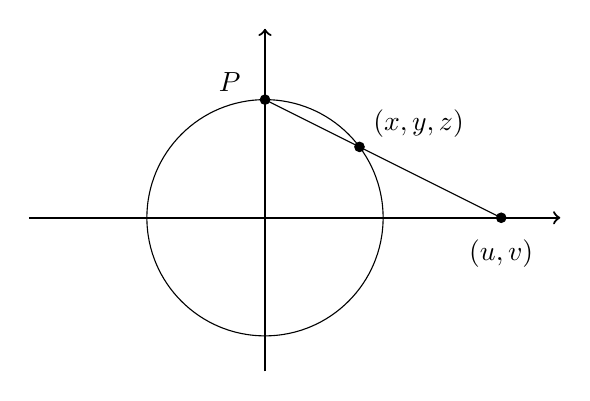
\begin{tikzpicture}[scale = 1.5]
		\draw[thick, ->] (-2,0) -> (2.5,0);
		\draw[thick, ->] (0,-1.3) -> (0,1.6);
		\draw (0,1) -> (2,0);
		\draw (0,0) circle (1);
		\draw[fill] (0,1) circle (0.04);
		\node at (-0.3,1.15) {$P$};
		\draw[fill] (0.8,0.6) circle (0.04);
		\node at (1.3,0.8) {$(x,y,z)$};
		\draw[fill] (2,0) circle (0.04);
		\node at (2,-0.3) {$(u,v)$};
	\end{tikzpicture}
	\caption{A two dimensional slice of a stereographic projection}
	\label{fig:StereographicProjection}
\end{figure}

In contrast to the linear case, admitting such a parametrization is a very restrictive condition on a system of polynomial equations. Rationality questions are concerned with studying when such a parametrization exists. 

There are also many interesting notions of being ``close to'' parametrizable by affine space. Contributing to the study of how these notions relate to each other, and how one can prove the nonexistence of such a parametrization, is an overarching goal of this thesis. As we will see, tools from many branches of mathematics can be applied to rationality questions. Algebraic tools are of course crucial to any work in algebraic geometry, but since we will primarily work over the complex numbers, we will also draw on ideas from topology and differential geometry.

\section{The Rationality Hierarchy}
To formalize the discussion above, we introduce some basic concepts from birational geometry. Let $X$ and $Y$ be varieties over a field $k$. A rational map $f \from X \ratmap Y$ is a morphism $f \from U \to Y$, where $U \subset X$ is a nonempty open set. The rational map $f \from X \ratmap Y$ is a birational map, written $f \from X \birat Y$, if there is a rational map $g \from Y \ratmap X$, such that both $g \circ f$ and $f \circ g$ are the identity map on an open set where both maps are defined.

We call a variety rational if it is parametrizable in the following sense.
\begin{definition}
	\label{def:Rational}
	A variety $X$ over a field $k$ of dimension $n$ is \emph{rational} if there exists a birational map $f \from \P^n \birat X$. Equivalently, the function field $k(X)$ is a purely transcendental extension of $k$.
\end{definition}
Affine space is an open dense subset of $\P^n$, so a rational variety is also parametrized almost everywhere by affine space. However, it is more convenient to work with projective space.

To describe varieties that are not rational, we will use the terms \emph{irrational} and \emph{nonrational} interchangeably.

Recall that a rational map $f \from X \ratmap Y$ is \emph{dominant} if its image is dense. A weaker version of being parametrizable by $\P^n$ is the following.
\begin{definition}
	\label{def:Unirational}
	Let $k$ be a field of characteristic 0. A variety $X$ over a field $k$ of dimension $n$ is \emph{unirational} if there exists a dominant rational map $f \from \P^m \ratmap X$. Equivalently, the function field $k(X)$ is a subfield of a purely transcendental extension of $k$.
\end{definition}
\begin{remark}
	If any such dominant map $f$ exists, and the field $k$ is infinite, then one may assume that $f$ is a generically finite morphism by restricting $f$ to a general linear subspace $\P^n \subset \P^m$ of suitable dimension.
\end{remark}
Starting from these two classical properties, a hierarchy of rationality properties has been studied, each capturing different notions of when a variety $X$ is close to being rational. We collect and motivate three important such properties here.
\begin{definition}
	\label{def:StablyRational}
	A variety $X$ is \emph{stably rational} if $X \times \P^m$ is rational for some $m$. Equivalently, there exists a purely transcendental extension $k(X)(t_1,\dots,t_m)$ of $k(X)$, such that this extension is a purely transcendental extension of $k$.
\end{definition}
Stable rationality traces its roots back to the following question by Zariski.
\begin{question}[Zariski problem]
	\label{que:Zariski}
	Let $K$ and $K'$ be finitely generated fields over a field $k$ such that there exists simple transcendental extensions of $K$ and $K'$ that are isomorphic. Must then $K$ and $K'$ be isomorphic?
\end{question}

There is also an associated equivalence relation, where we say that two varieties, $X,Y$, are \emph{stably birational}, or \emph{stably birationally equivalent}, if $X \times \P^n \birat Y \times \P^m$ for some $n,m$. We say that an invariant associated to a variety $X$ is a \emph{stable birational invariant} if it is preserved by stable birational equivalence.

\begin{definition}
	\label{def:RetractRational}
	A variety $X$ is \emph{retract rational} if there are rational maps $f \from X \ratmap \P^N$ and $g \from \P^N \ratmap X$ and an open subset $U \subset X$, such that $g \circ f$ is defined on $U$ and $g \circ f \from U \to U$ is the identity.
\end{definition}
The definition of retract rationality is the hardest one to motivate. It was originally introduced in an algebraic context by Saltman in \cite{SaltmanHomage}, with a goal of understanding how rationality relates to certain approximation properties. More geometrically, a natural question arising from the definition of stable rationality is whether a stably irrational variety $X$ could be a factor in a rational variety. It is not hard to see that if $X \times Y$ is rational for some variety $Y$, then $X$ is retract rational, so studying retract rationality can answer this question. Finally, retract rationality is interesting because of its relation to decompositions of the diagonal, see \cref{prop:RetractRationalDecomposition}. This makes it the natural rationality property to investigate with this powerful tool.

The final rationality property we introduce is rational connectedness.
\begin{definition}
	\label{def:RationallyConnected}
	A variety $X$ over an uncountable algebraically closed field $k$ is \emph{rationally connected} if for any two general points $y,x \subset X$ there is a map $\P^1_k \to X$, defined over $k$, such that $0 \mapsto x$ and $\infty \mapsto y$.
\end{definition}
Rational connectedness is a relatively weak property, but it is well-behaved and usually easy to check. For example, one can prove that in a family of smooth varieties, if the generic member is rationally connected, then every member is rationally connected. The corresponding statement for \eg unirationality is not known. Furthermore, if a smooth variety contains a rational curve with ample normal bundle, it is rationally connected, and in characteristic 0 a smooth Fano variety is rationally connected. Proofs of these statements can be found in \cite[IV.3, V.2]{KollarRationalCurves}.

We have the following straightforward implications between the five rationality properties we have introduced.
\begin{proposition}
	\label{prop:RationalityHierarchy}
	Let $X$ be a variety over a field $k$. Then each property in this list implies the next. %\todo{Add nice arrows?}
	\begin{enumerate}[i)]
		\item $X$ is rational.
		\item $X$ is stably rational.
		\item $X$ is retract rational.
		\item $X$ is unirational.
		\item $X$ is rationally connected.
	\end{enumerate}
\end{proposition}
Studying when, if at all, the converse implications hold, has been a major and fruitful area of birational geometry. For curves, clearly rationally connected implies unirational. Furthermore, by Lüroth's theorem, all five properties coincide.
\begin{theorem}[{Lüroth's theorem (\cite[Example 2.55]{Hartshorne})}] %\todo{Should I reference the original, or maybe not at all?}
	\label{thm:Lueroth}
	Let $k$ be a field, $t$ a transcendental element over $k$, and $k(t)/K/k$ field extensions. Then $K$ is also a purely transcendental extension of $k$.
\end{theorem}
In geometric language, \cref{thm:Lueroth} states that any unirational curve is rational. To see this geometric implication, assume that $X$ is a curve and $f \from \P^1 \ratmap X$ is a rational map. Then we have the following tower of field extensions: $k(t)/k(X)/k$. By \cref{thm:Lueroth}, $k(X)$ must be a purely transcendental extension of $k$ of degree $1$, hence $k(X) \simeq k(t)$. So the curve $X$ must be rational. Because of this result, studying the relationship between unirationality and rationality has been known as the \emph{Lüroth problem}.

A major achievement of the Italian school of algebraic geometry is the proof that for smooth surfaces over an algebraically closed field of characteristic 0, the five properties in \cref{prop:RationalityHierarchy} are also equivalent. To see this, one first checks that if $X$ is rationally connected, then there is a dominant map $f \from C \times \P^1 \ratmap X$ for some curve $C$. This implies that all plurigenera of $X$ are zero, so $X$ is rational by Castelnuovo's criterion for rationality (\cite[V.6.2]{Hartshorne}). In positive characteristic however, unirational surfaces that are not rational exist. Examples of this were found by Zariski (see \cite{Zariski58}).

Starting from dimension 3, the properties in \cref{prop:RationalityHierarchy} are no longer equivalent, even over $\C$. Already in the early twentieth century Fano claimed to have found an example of a unirational, non rational threefold. However, the proof contained gaps.
%have a proof that the intersection of a quadric and a cubic hypersurface in $\P^5$, which is a unirational variety, is not rational. However the proof contained gaps. Later, Roth claimed to construct a complex unirational variety which was not simply connected, and hence not rational. However, also this proof contained errors, and  Serre later proved that any complex unirational variety is simply connected. %\todo{Keep this historical note?}
Thus, the answer would first come in the early 1970s; three examples appeared independently of irrational, unirational threefolds.

First, following the original ideas of Fano, Iskovskikh and Manin proved
in \cite{IskovskikhManin}
that any birational automorphism of a smooth quartic threefold is in fact biregular. On the other hand, $\P^3$ has infinitely many birational, but not biregular, automorphisms. Therefore, a smooth quartic threefold cannot be rational.
%the following.
% \begin{theorem}[{\cite{IskovskikhManin}}]
	% 	\label{thm:QuarticRigidity}
	% 	Let $X \subset \P^4$ be a smooth quartic threefold, then any birational automorphism of $X$ is in fact a biregular automorphism. In particular, $X$ is not rational.
	% \end{theorem}
% The implication that $X$ is irrational follows since $\P^n$ has infinitely many birational, but not biregular, automorphisms.
In \cite{SegreVariazioneContinua}, Segre had constructed a smooth, unirational quartic hypersurface, so this gave the first counterexample to the Lüroth problem.

Around the same time, Clemens and Griffiths introduced
in \cite{ClemensGriffiths}
a rationality criterion based on the intermediate Jacobian and used it to prove that no smooth cubic threefold is rational.
% the following rationality criterion.
% \begin{theorem}[{\cite{ClemensGriffiths}}]
	% 	Let $X$ be a smooth rational threefold. Then its intermediate Jacobian is the product of Jacobians of curves.
	% \end{theorem}
% They also apply the criterion to cubic threefolds.
% \begin{theorem}[{\cite{ClemensGriffiths}}]
	% 	\label{thm:CubicThreefoldIrrational}
	% 	The intermediate Jacobian of a smooth cubic threefold is not a product of Jacobians of curves, and therefore irrational.
	% \end{theorem}
Projecting from any line in a cubic threefold gives the threefold a conic bundle structure, hence a smooth cubic threefold is unirational. These examples prove that even over $\C$, the properties in \cref{prop:RationalityHierarchy} are no longer equivalent,  starting from dimension 3.

However, the obstructions to rationality used by
Iskovskikh-Manin and Clemens-Griffiths
only obstruct rationality, and not the weaker properties in \cref{prop:RationalityHierarchy}. So more examples are necessary to understand the relation between the various other rationality properties.

Shortly after the work of Iskovskikh-Manin and of Clemens-Griffiths appeared, Artin and Mumford constructed one such example.
\begin{theorem}[{\cite{ArtinMumford}}]
	\label{thm:ArtinMumfordIntroduction}
	There exists a unirational double cover $X \to \P^3$, admitting a desingularization $\widetilde{X} \to X$, such that $H^3(\widetilde{X},\Z)$ has nontrivial torsion. Since this torsion group is a stable birational invariant of smooth complex varieties, $\widetilde{X}$ is not stably rational.
\end{theorem}
We will soon see that this invariant proves that $X$ has no decomposition of the diagonal, and is therefore also not retract rational. Although these concepts were not introduced at the time of \cite{ArtinMumford}, \cref{thm:ArtinMumfordIntroduction} also proves that retract rationality is a stronger property than unirationality.

Regarding the relation between rationality and stable rationality, Beauville, Colliot-Thélène, Sansuc and Swinnerton-Dyer answered \cref{que:Zariski} negatively over $\C$. In the paper \cite{BCTSSD} they find a smooth, irrational, complex threefold $X$ such that $X \times \P^3$ is rational. In fact, Shepherd-Barron proves in \cite{Shepherd-Barron} that also $X \times \P^2$ is rational. As far as the author is aware, this is essentially the only known example of an irrational, but stably rational, complex variety.

These examples prove that most of the implications in \cref{prop:RationalityHierarchy} are not equivalences. The following two questions remain.
\begin{question}
	\label{que:StableVsRetract}
	Does there exist a retract rational variety over an algebraically closed field that is not stably rational?
\end{question}

\begin{question}
	\label{que:RationallyConnectedVsUnirational}
	Does there exist a rationally connected variety that is not unirational?
\end{question}
Especially the latter question is a major open problem in birational geometry. The answer to both of these questions is widely expected to be positive, but constructing examples illustrating this has proven to be difficult.

\section{Retract Rationality and Unirationality of Certain Complete Intersections}
The papers in the thesis fall into two categories. The three first papers fall into the first category, namely studying rationality properties of certain simple varieties. The thesis begins with two papers proving retract irrationality of two complete intersections in projective space. The third paper studies unirationality of double covers and complete intersections of quadrics.

\subsection{Specialization and Decomposition of the Diagonal}
% A large part of the difficulty in distinguishing the properties in \cref{prop:RationalityHierarchy}, lies in finding invariants that obstruct some, but not all of the properties. So for any (stably) birational invariant, it is an interesting question if it can be nontrivial on rationally connected varieties.

%In this thesis, we will focus on other invariants, which are potentially useful in higher dimensions. We will focus on understanding these invariants on so-called Fano varieties. Recall that a variety $X$ is called a \emph{Fano variety} if the anticanonical divisor $-K_X$ is ample. It is a celebrated result by Mori that in characteristic 0, any Fano variety is rationally connected. In particular, we will concentrate on some central examples of Fano varieties, hypersurfaces, complete intersections and double covers. The space of rational curves on a Fano variety $X$ contains much information about the geometry of $X$. And in the later sections of the thesis, we focus on birational invariants related to curves on $X$, and how studying the space of rational curves lets us compute these invariants. \todo{Maybe this general principle should be emphasized more?}
We first introduce the concept of a \emph{decomposition of the diagonal}. This plays the main role in \cref{pap:23diagonal} and \cref{pap:33diagonal}. It also has strong implications for all the the other rationality properties and birational invariants we study throughout the thesis. Decomposition of the diagonal with rational coefficients were introduced in by Bloch and Srinivas in \cite{BSCorrespondences}. Beginning with Voisin's landmark paper \cite{VoisinDoubleQuartic}, its relation to rationality properties has attracted much attention.
\begin{definition}
	\label{def:DoD}
	Let $X$ be a scheme of pure dimension $n$. We say that $X$ admits a (Chow theoretic) \emph{decomposition of the diagonal} if the following equality holds in $\CH_n(X \times X)$, with coefficients in $\Z$,
	\begin{equation}
		\label{eq:DefinitionDoD}
		[\Delta_X] = [X \times z] + [W].
	\end{equation}
	Here $z \in X$ is a zero cycle of degree 1 and $W$ is supported on $D \times X$, with $D \subsetneq X$ a closed subscheme of $X$.
\end{definition}
If \eqref{eq:DefinitionDoD} holds in $\CH(X \times X) \otimes \Q$ instead, we say that $X$ admits a \emph{decomposition of the diagonal with rational coefficients}.
%If such an equality holds in the cohomology ring $H^*(X \times X,\Z)$ instead, we say that $X$ admits a cohomological decomposition of the diagonal.

% For proper varieties there is also the following alternative viewpoint.
% \begin{definition}
% 	Let $X$ be a proper variety over a field $k$. We say that the Chow group of zero-cycles $\CH_0(X)$ is \emph{universally trivial} if for any field extension $K/k$, the degree map $\deg \from \CH_0(X_K) \to \Z$ is an isomorphism.
% \end{definition}
% \begin{proposition}[{\cite[Proposition 1.4]{ColliotThelenePirutka}}]
% 	\label{prop:DecompositionCH0Trivial}
% 	A smooth, proper, geometrically integral variety $X$ has a decomposition of the diagonal if and only if $\CH_0(X)$ is universally trivial.
% \end{proposition}

A decomposition of the diagonal is closely related to three of the properties in \cref{prop:RationalityHierarchy}. We summarize this connection with three results. For proofs and references to the papers where these concepts and results first appeared, see Schreieder's excellent survey \cite{SchreiederCyclesAndRationality}.
\begin{proposition}[{\cite[Section 7.2]{SchreiederCyclesAndRationality}}]
	If a variety $X$ is rationally connected, then there exists an integer $N$, such that $N[\Delta_X]$ has a decomposition as in \eqref{eq:DefinitionDoD}.
\end{proposition}
%
%\begin{definition}
%	For a proper variety $X$, the smallest positive integer $N$ such that $N[\Delta_X]$ admits a decomposition of the diagonal, is known as the \emph{torsion order}, and is a stable birational invariant of smooth varieties.
%\end{definition}

\begin{proposition}[{\cite[Corollary 7.12]{SchreiederCyclesAndRationality}}]
	If there is a dominant map $\P^n \ratmap X$ of degree $N$ \ie $X$ has a unirational parametrization of degree $N$, then $N[\Delta_X]$ has a decomposition as in \eqref{eq:DefinitionDoD}.
\end{proposition}
%Mention that this $N$ is called the torsion order

\begin{proposition}[{\cite[Lemma 7.4]{SchreiederCyclesAndRationality}}]
	\label{prop:RetractRationalDecomposition}
	If $X$ is retract rational, then $X$ has a decomposition of the diagonal.
\end{proposition}

Also, if a variety $X$ admits a decomposition of the diagonal, this forces many birational invariants to be trivial. We illustrate the principle with the following result and proof.
\begin{proposition}[{\cite[Theorem 3.4]{VoisinAbelJacobi}}]
	\label{thm:DecompositionAndH3}
	Let $X$ be a complex threefold admitting a decomposition of the diagonal, then $H^3(X,\Z)$ has no torsion.
\end{proposition}
\begin{proof}
	If we think of both sides of \eqref{eq:DefinitionDoD} as representing self-correspondences of $X$, they both act on $H^3(X,\Z)$. The left hand side acts as the identity, and the action of the right hand sides takes classes in $H^3(X,\Z)$ to classes in $H^1(\widetilde{W},\Z)$, for some desingularization $\widetilde{W}$ of $W$. This cannot have any torsion. Hence, the image of the identity map on $H^3(X,\Z)$ has no torsion.
\end{proof}
This proves that the variety $\widetilde{X}$ from \cref{thm:ArtinMumfordIntroduction} does not admit a decomposition of the diagonal. Hence, by \cref{prop:RetractRationalDecomposition}, it is not retract rational.

\begin{remark}
	There are smooth, irrational varieties that admit a decomposition of the diagonal (see \cite{ColliotThelenePresqueDiagonales}), but it is an open question if there are smooth, non retract rational varieties with a decomposition of the diagonal.
\end{remark}

We can now set the stage for the first two papers in this thesis. Starting with Koll\'ar's paper \cite{KollarHypersurfaces}, specialization methods have been used to study rationality questions. The basic idea is that we can prove irrationality of a given variety $X$ by finding a reference variety $X_0$ with some nontrivial birational invariant and a specialization of $X$ to $X_0$ that preserves this birational invariant.

There are three main such specialization methods, detecting increasingly strong rationality properties. The method from \cite{KollarHypersurfaces} is based on ruledness (being birational to a product $Y \times \P^1$). The important point is that ruledness is preserved under specialization. For complex hypersurfaces of sufficiently large degree, Koll\'ar constructs a specialization to a variety in positive characteristic that admits a global differential form. This special variety can therefore not be ruled, and hence the general fiber is likewise not ruled. With this strategy, Koll\'ar proves that a very general complex hypersurface in $\P^{n+1}$ of degree $\frac{2}{3}(n+3)$ is not ruled, and hence not (stably/retract) rational.

A breaktrough in specialization methods was introduced by Voisin in \cite{VoisinDoubleQuartic}. The important point is that having a decomposition of the diagonal is preserved under specialization, as long as the special fiber satisfies certain smoothness conditions. This is in contrast to many other birational invariants, such as torsion in $H^3(X,\Z)$. By specializing a very general double quartic solid to the example of Artin and Mumford, Voisin proves that the special fiber cannot have a decomposition of the diagonal. Hence, the very general fiber cannot have a decomposition of the diagonal, and is therefore retract irrational.

This specialization technique was then developed further by Colliot-Thélène and Pirutka in \cite{ColliotThelenePirutka} and by Schreieder in \cite{SchreiederHypersurface}, proving retract irrationality of a very general quartic threefold, and hypersurfaces in $\P^{n+1}$ of degree at least $\log_2 n + 2$, respectively.

The final specialization method relevant here is based on the motivic volume introduced by Nicaise and Shinder in \cite{NicaiseShinderMotivic}. This was developed further by Kontsevich and Tschinkel in \cite{KontsevichTschinkelSpecialization} and by Nicaise and Ottem in \cite{NicaiseOttemRefinement}. The motivic volume was used by Nicaise and Ottem in \cite{NicaiseOttem} to prove stable irrationality of many complete intersections whose irrationality was previously unknown.

The specialization method is based on the ring of stable birational types; equivalence classes under stable birational equivalence. In this ring, the sum and product are induced by disjoint unions and Cartesian products, respectively. If a specialization of a variety over a field of characteristic 0 is not too singular, there is a ring homomorphism taking the stable birational type of the generic fiber to the stable birational type of the special fiber. So if the stable birational type of the special fiber is nontrivial, the stable birational type of the generic fiber must be nontrivial as well. Because of the ring structure, this technique is particularly well suited to specializing to fibers with multiple components.

The specialization methods outlined above are powerful, but they all require as input some example where irrationality can be verified in another way. For this, other birational invariants are required. One such invariant is the unramified cohomology group $H_{nr}^2(k(X)/k,\mu_2^{\otimes 2})$. This stable birational invariant is closely related to torsion in $H^3(X,\Z)$ (c.f. \cref{thm:ArtinMumfordIntroduction}). In fact, for smooth varieties this particular unramified cohomology group is isomorphic to the cohomological Brauer group, which in turn is isomorphic to torsion in $H^3(X,\Z)$. A reason to use this particular birational invariant is the remarkable example found by Hassett, Pirutka and Tschinkel in \cite{HPTActa} of a quadric surface bundle $X \to \P^2$ with nontrivial unramified cohomology. This quadric surface bundle has proven to be a very useful target for specializations.

\subsection{Summary of \cref{pap:23diagonal}}
The three specialization techniques outlined above preserve different rationality properties. So comparing the three techniques can potentially shed light on how the corresponding rationality properties can differ. In light of the question of whether stable and retract rationality are equivalent over algebraically closed fields (\cref{que:StableVsRetract}), it is particularly interesting if the specialization method based on decomposition of the diagonal is applicable to the examples where stable rationality was first proven in \cite{NicaiseOttem}. One such example is the complete intersection of a quadric and a cubic hypersurface in $\P^6$. Since these are known to be stably irrational, they are natural candiates for examples of retract rational but stably irrational varieties, the existence of which is still unknown over algebraically closed fields.

In \cref{pap:23diagonal}, we use the specialization technique based on decomposition of the diagonal to prove that the very general intersection of a quadric and a cubic hypersurface in $\P^6$ is not retract rational. With this result, the cubic fourfold is the only complete intersection in dimension 4
for which retract rationality of a very general member remains open.

 An additional goal of \cref{pap:23diagonal} is to find explicit examples of retract irrational complete intersections, complementing the result about the very general intersection. Specifically, we find examples defined over countable fields, such as $\Q$, of non retract rational complete intersections of a quadric and cubic hypersurface in $\P^6$. To find examples over countable fields, it is necessary to specialize to positive characteristic.

The main result of the paper is.
\begin{theorem}
	\label{thm:SpecializationIntroduction}
	Let $K=\Q$ or $K=\F_p(t)$ with $p \geq 3$. In the first case let $p \geq 3$, $q \geq 11$ be distinct primes and set $u=p,v=q$, and in the second case let $u=t,v=(t-1)$. Let $X \subset \P^6_K$ be the complete intersection defined by the following two equations:
	\begin{equation}
		\ u \left(\sum_{i=0}^6 x_i^2 \right) + v(x_3x_6-x_4x_5)=0
	\end{equation}
	
	\begin{align}
		u \left(\sum_{i=0}^6 x_i^3 \right) + v(x_0^2x_5 &+ x_1^2x_4 + x_2^2x_6 \nonumber \\
		 &+ x_3(x_5^2+x_4^2+x_3^2 -2x_3(x_6 + x_5 + x_4)))=0.
	\end{align}
	Then $X$ is a smooth complete intersection such that the base change to $\overline{K}$ does not admit a decomposition of the diagonal. It is therefore not geometrically retract rational.
\end{theorem}
\begin{remark}
	Since the complete intersection $X$ in \cref{thm:SpecializationIntroduction} is smooth, it is straightforward to use a second specialization argument to prove that the very general complete intersection of a cubic and quadric hypersurface in $\P^6$ over $\C$ is not retract rational.
\end{remark}
We prove \cref{thm:SpecializationIntroduction} using a specialization heavily inspired by the one used in \cite{NicaiseOttem}. The complete intersection is specialized to a complete intersection singular along a plane. After blowing up the plane, one obtains a variety birational to the quadric surface bundle from \cite{HPTActa}. The exceptional locus of the blowup is a rational quadric bundle. To obstruct the existence of a decomposition of the diagonal on this union we rely heavily on the techniques in \cite{SchreiederHypersurface}. The main point is identifying a nontrivial unramified cohomology class on the blowup, namely the one found in \cite{HPTActa}. This nontrivial class obstructs a decomposition of the diagonal on the special fiber. The main innovation in \cref{pap:23diagonal} lies in using the unramified cohomology class on the blowup of the special fiber to prove that the special fiber itself does not admit a decomposition of the diagonal. Additionally, there is some work involved in picking the exact equations and verifying the technical details for this particular choice.

\subsection{The Specialization Technique of Pavic and Schreieder}
The specialization method in \cref{pap:23diagonal} is also applicable when specializing to a union of two varieties. However, it is crucial that the obstruction to rationality lies on one of the components of the special fiber. The intersection of the components must be rational, or at least the obstruction to rationality should vanish on the intersection.

Contrast this with the method in \cite{NicaiseOttem}, which also works well when specializing such that two rational components meet in a stably irrational locus. In fact, such specializations often give the most powerful results. Especially in higher dimensions, this flexibility lets one prove stable irrationality of many complete intersections. By specializing to a union whose intersection is stably irrational, Nicaise and Ottem prove that for the following four complex fivefolds, the very general such fivefold is stably irrational: the quartic fivefold, the intersection of two cubics in $\P^7$, the intersection of two quadrics and a cubic in $\P^8$ and finally the intersection of four quadrics in $\P^9$.

Since the specialization method of Nicaise and Ottem does not say anything about retract rationality, studying retract rationality of these fivefolds is an interesting problem. With this in mind, Pavic and Schreieder develop in \cite{PavicSchreieder} a new obstruction to the existence of a decomposition of the diagonal. This obstruction is suitable for specializations to a union where the intersection does not admit a decomposition of the diagonal. Working with this obstructions is quite technical, but very broadly, the main idea is to study the $\CH_1$ group of the special fiber.
%The nature of the obstruction is summarized well by the following result.
%\begin{theorem}[{\cite[Corollary 1.3]{PavicSchreieder}}]
%	\label{thm:PSCorollaryIntro}
%	Let $R$ be a DVR with algebraically closed residue field $k$ and let $\pi \from \mathcal{X} \to \Spec R$ be a projective semi-stable $R$-scheme whose special fiber $Y = Y_1 \cup Y_2$ has two components. Assume that
%	\begin{itemize}
%		\item $Y$ is universally $\CH_1$-trivial in the sense that for any field extension $L/k$, the natural map $\CH_1(Y) \to \CH_1(Y_L)$ is surjective;
%		\item $Y_{12} \coloneqq Y_1 \cap Y_2$ is integral and its torsion order is even.
%	\end{itemize}
%	Then the geometric generic fiber of $\pi$ does not admit a decomposition of the diagonal.
%\end{theorem}
In \cite{PavicSchreieder}, Pavic and Schreieder also apply this obstruction to prove that over an algebraically closed field of characteristic different from $2$, the very general quartic fivefold does not admit a decomposition of the diagonal, and is therefore not retract rational.

\subsection{Summary of \cref{pap:33diagonal}}
Comparing the obstructions in \cite{NicaiseOttem} and \cite{PavicSchreieder} is a very interesting question, since they detect different kinds of rationality and are, at least a priori, unrelated. A natural starting point is to check if the techniques in \cite{PavicSchreieder} suffice to prove retract irrationality of the fivefolds whose stable irrationality was first proven in \cite{NicaiseOttem}. The goal of \cref{pap:33diagonal} is to take a step in this direction by applying the method of \cite{PavicSchreieder} to the very general intersection of two cubics in $\P^7$.

The core idea in the specialization is the same as in \cite[Theorem 7.2]{NicaiseOttem}. By specializing one of the cubics to the union of a hyperplane and a quadric, the special fiber is a union of two components meeting along the intersection of a quadric and a cubic in $\P^6$. From \cref{pap:23diagonal}, we know this variety is not retract rational. After setting up this specialization, a technical section follows where we check that the obstruction from \cite{PavicSchreieder} can be applied, which proves that the very general intersection of two cubic sixfolds does not admit a decomposition of the diagonal.

The technical work consists of two specializations. First we modify a naïve specialization to a union of two components through a series of blowups, such that the obstruction of Pavic and Schreieder applied. In a second part, we further specialize the special fiber to better control $\CH_1$ of the two components. The main tool is specializing such that the components become rational, which simplifies $\CH_1$. Throughout we follow the argument in \cite{PavicSchreieder} very closely. The main novel contribution of \cref{pap:33diagonal} lies in finding a concrete specialization of an intersection of two cubic sixfolds, and further showing how we can simplify $\CH_1$ to apply the obstruction from \cite{PavicSchreieder}. We obtain the following theorem:
\begin{theorem}
	Let $k$ be an uncountable algebraically closed field of characteristic $0$. Then the very general complete intersection of two cubic hypersurfaces in $\P^7_k$ does not admit a decomposition of the diagonal, and is therefore not retract rational.
\end{theorem}
In this paper, we only work over characteristic $0$ to keep the proofs slightly less technically demanding. But, as is explained in \cref{pap:33diagonal}, only small modifications of the proof are necessary to prove the main result over an algebraically closed field of characteristic different from $2$ and $3$.

\subsection{Unirationality in High Dimensions}
We next turn our attention to unirationality. Here we also first encounter double covers of projective space. This is another classical construction of algebraic varieties and will play an important role in the remainder of the thesis.

Let $X$ be a hypersurface, a complete intersection or a double cover. It is natural to ask how the rationality properties of $X$ depend on the degree and dimension of $X$. In one direction, we want a lower bound on the degree, depending on the dimension of $X$, such that if the degree of $X$ exceeds this bound, a general $X$ does not have a given rationality property. In this direction, Schreieder has found a logarithmic bound on the degree of hypersurfaces, such that the very general hypersurface of degree exceeding this bound is not retract rational (\cite{SchreiederHypersurface}). For double covers, or more generally cyclic covers, the same question has been studied by Okada in \cite{OkadaCyclicCovers} and by Schreieder in \cite[Theorem 9.1]{SchreiederHypersurface}.

%  Okada proves in \cite[Theorem 1.1]{OkadaCyclicCovers} that a very general cyclic cover $p \from X \to \P^n$ of dimension $n \geq 3$ and branched along a hypersurface of degree $d \geq n+1$, is not stably rational. Schreieder remarks in \cite{SchreiederHypersurface} that the techniques developed in that paper give the following result for double covers.
% \begin{theorem}[{\cite[Theorem 9.1]{SchreiederHypersurface}}]
	%   Let $N \geq 3$ be a positive integer, and write $N = n+r$ with $2^{n-1}-2 \leq r \leq 2^n-2$. Let $k$ be an uncountable field of characteristic different from two. Then a double cover of $\P_k^N$ branched along a very general hypersurface of even degree $d \geq 2\lceil \frac{n+1}{2}\rceil + 2$ is not stably rational over the algebraic closure of $k$.
	% \end{theorem}
% This gives a logarithmic bound in the dimension $N$ on the degree $d$ such that the very general double cover of degree at least $d$ is not stably rational, improving on the linear bound in \cite{OkadaCyclicCovers}.
% \begin{remark}
	%   Since the argument is based on decomposition of the diagonal, it in fact proves retract irrationality of these double covers.
	% \end{remark}

In the other direction, we could fix a degree $d$ and ask how big must the dimension $n$ be such that any smooth, or a general, hypersurface or double cover has some rationality property. The simplest case is rational connectedness. We see by adjunction that any smooth hypersurface $X \subset \P^n$ of degree $d \leq n$ is Fano, and it is therefore rationally connected, at least over a field of characteristic 0.

In contrast, asking this question about unirationality turns out to be quite subtle, and it has attracted attention for a long time. For hypersurfaces, this question has been studied first by Morin in \cite{MorinUnirationality}. There it is asserted that for any fixed degree $d$, a general hypersurface of degree $d$ is unirational if its dimension exceeds some bound $\eta(d)$. The bounds on the dimension in \cite{MorinUnirationality} were later improved and made more explicit by Ramero in \cite{Ramero}. Later, Harris, Mazur and Pandharipande proved in \cite{HMPUnirationality} that the same result holds for any smooth hypersurface, and better bounds on the dimension were found by Beheshti and Riedl in \cite[Corollary 4.6]{BRHypersurface}.

The same question can be asked for double covers. In \cite{CMMDoubleCover}, Conte, Marchiso and Murre use an idea of Ciliberto to prove that for sufficiently large dimension compared to the degree, the general double cover of $\P^n$ is unirational. The argument is analogous to the one used by Morin and Ramero.

\subsection{Summary of \cref{pap:unirationality}}
In this short note, we prove some results on unirationality in the spirit of Morin. Firstly, we prove the following for double covers:
\begin{theorem}
	Let $k$ be an algebraically closed field of characteristic 0. Then for any positive integer $d$ there is an integer $\eta'(d)$, such that any smooth double cover of projective space ramified over a hypersurface of degree $d$ and of dimension at least $\eta'(d)$ is unirational. Furthermore, $\eta'(d) \leq 2^{(2d)!} - 1$.
\end{theorem}
This generalizes the result in \cite{CMMDoubleCover} to any smooth double cover. The proof is essentially a one-liner. We use the fact that for any smooth double cover of $\P^n$ ramified over a hypersurface of degree $2d$, one can construct a smooth hypersurface $Y \subset \P^{n+1}$, with a dominant morphism $Y \to X$. Since $Y$ is a smooth hypersurface, we know that it is unirational for sufficiently large dimension $n$. Then $X$ is likewise unirational.

Secondly, we study unirationality of complete intersections of $K$ quadrics in $\P^N$, defined over an algebraically closed field $k$ of characteristic different from 2. We obtain the following result:
\begin{theorem}
	\label{thm:QuadricsUnirationalityIntroSection}
	Let $X_{K,N}$ be an irreducible complete intersection of $K$ quadrics in $\P_k^N$ of dimension at least 1. If 
	\[\frac{K^2}{2} + K - 2 \leq N,\]
	then $X_{K,N}$ is unirational.
\end{theorem}
We prove this by generalizing a construction by Beauville for three quadrics in $\P^6$. The construction works for $K$ quadrics as long as their intersection contains a $(K-2)$-plane. This condition gives the bound in \cref{thm:QuadricsUnirationalityIntroSection}. One should compare this bound to the bound for rational connectedness.
\begin{proposition}
	\label{prop:QuadricsRationalConnectednessIntroSection}
	Let $X_{K,N}$ be a smooth complete intersection of $K$ quadrics in $\P_k^N$. Then $X$ is rationally connected if and only if $2K \leq N$.
\end{proposition}
Also compare \cref{thm:QuadricsUnirationalityIntroSection} to a bound for rationality, likewise based on $X_{K,N}$ containing a linear space of large dimension.
\begin{theorem}
	\label{thm:QuadricRationalBoundIntroSection}
	Let $X_{K,N}$ be the complete intersection of $K$ quadrics in $\P_k^N$. If
	\[ \frac{K^2}{2} + \frac{3K}{2} - 1 \leq N,\]
	then $X_{K,N}$ is rational.
\end{theorem}
Together, these three bounds give a range of possible candidates for complete intersections of quadrics $X_{K,N}$, where $X_{K,N}$ has some, but not all, of the properties in the rationality hierarchy of \cref{prop:RationalityHierarchy}.


\section{Birational Invariants on Some Rationally Connected Varieties}
In the remaining papers, we turn to investigating specific birational invariants on a complex variety $X$. Placing a given rationally connected variety at the appropriate level of the hierarchy in \cref{prop:RationalityHierarchy} is a hard problem. To do so, one usually needs a birational invariant that obstructs one of the stronger properties, like rationality or unirationality, but can be nontrivial on rationally connected varieties. It is therefore an interesting question if a given (stable) birational invariant is necessarily trivial on any rationally connected variety, or on any rationally connected variety of a given class.

We will not study this question on arbitrary rationally connected varieties, but focus on some central examples, namely Fano complete intersections and double covers over $\C$. It is a consequence of Mori's celebrated bend and break method that any smooth Fano variety is rationally connected.

The three invariants we study have no direct relation but share some common features. They all arise by comparing the topological and algebraic structure on a complex variety $X$ and are closely related to curves on $X$.

\subsection{The Integral Hodge Conjecture}
The first such invariant we investigate arises from the Integral Hodge Conjecture.

\begin{definition}[{\cite[Definition 2.14]{VoisinLueroth}}]
	\label{def:ZInvariant}
	Let $X$ be a complex variety of dimension $n$, and let $\xi \from H^{2n-2}(X,\Z) \to H^{2n-2}(X,\C)$ be the map on Betti cohomology given by changing coefficents. We have a Hodge decomposition 
	\[H^{2(n-i)}(X,\C) = \bigoplus_{p+q=2(n-i)}H^{p,q}(X,\C).\]
	Define the \emph{integral Hodge classes} 
	\[H^{n-i,n-i}(X,\Z) \coloneqq \xi^{-1}(H^{n-i,n-i}(X,\C)) \subset H^{2(n-i)}(X,\Z).\]
\end{definition}
\begin{definition}
	We say that the \emph{Integral Hodge Conjecture} holds for $i$-cycles on $X$, if the integral Hodge classes $H^{n-i,n-i}(X,\Z)$ are generated by the classes of $i$-dimensional algebraic subvarieties of $X$.
\end{definition}

If $X$ is a smooth complex variety, and the Integral Hodge Conjecture holds for $1$-cycles or for codimension $2$ cycles, then the same is true for any smooth complex variety $Y$ stably birational to $X$. So two birational invariants arise from the Integral Hodge Conjecture. In fact, the quotients of $H^{2,2}(X,\Z)$ and of $H^{n-1,n-1}(X,\Z)$ by the subgroup generated classes of algebraic cycles are stable birational invariants.

We will focus on the Integral Hodge Conjecture for $1$-cycles, but the Integral Hodge Conjecture for codimension $2$ cycles has also attracted much attention and has a connection to unramified cohomology (see \cite{ColliotTheleneVoisinIntegralHodge}).

The first counterexamples to the Integral Hodge Conjecture for $1$-cycles were found by Atiyah and Hirzebruch in \cite{AtiyahHirzebruch}. It is clear that on a smooth complex variety $X$, the torsion classes of $H^{2n-2}(X,\Z)$ are integral Hodge classes.  Atiyah and Hirzebruch construct examples of varieties with nonalgebraic torsion classes in $H^{2n-2}(X,\Z)$.

A different approach is used for the so-called "Trento examples" in \cite{KollarTrento}. There Koll\'ar proves that if $k\geq 4$ is coprime to 6, and $X \subset \P^4$ is a very general hypersurface of degree $k^2$, then the degree of any curve in $X$ is divisible by $k$. Since $H^{n-1,n-1}(X,\Z)$ contains a cohomological class of degree 1 by the Lefschetz Hyperplane Theorem, the Integral Hodge Conjecture must fail. So the Integral Hodge Conjecture can fail even for varieties with no torsion in $H^{2n-2}(X,\Z)$.

In both cases, the counterexamples are of general type, and therefore not rationally connected.  It is an interesting question how close to rational a variety can be and still not satisfy the Integral Hodge Conjecture. In \cite{BenoistOttemIntegralHodge}, a threefold of Kodaira dimension 0 is constructed, on which the Integral Hodge Conjecture fails. Furthermore, in \cite{OttemSuzukiPencil} and \cite{OttemSuzukiAcyclic} Ottem and Suzuki construct examples of varieties where the Integral Hodge Conjecture fails and $\CH_0(X) = \Z$. However, so far no rationally connected counterexample to the Integral Hodge Conjecture is known. In \cite{SouleVoisin}, Soulé and Voisin raise the question if the conjecture holds for any rationally connected variety.

Beyond this question, it is not even known if the Integral Hodge Conjecture can fail for varieties with trivial canonical divisor, so called \CY varieties. These varieties are not a main focus of this thesis but can be thought of as lying on the boundary between Fano varieties and varieties of general type. \CY varieties have a rich geometry and have been widely studied. Originally, \cref{pap:integralhodge} was motivated by a desire to understand the Integral Hodge Conjecture on an important class of \CY varieties, namely anticanonical hypersurfaces in smooth Fano toric varieties.

\subsection{Summary of \cref{pap:integralhodge}}
The goal of \cref{pap:integralhodge} is to prove that the integral Hodge Conjecture holds for a broad class of rationally connected varieties. The main theorem also applies to an important class of \CY varieties.

Up to this point, we have studied complete intersections in projective space, and double covers of projective space. To obtain a richer class of examples, we can study complete intersections in more general ambient varieties. Toric varieties are a good choice of ambient varieties generalizing projective space. These have a rich geometry but are still completely described by combinatorial objects, and therefore comparatively simple.

A natural approach to proving that the Integral Hodge Conjecture holds for a variety $X$, is to find a collection of algebraic curves in $X$, such that their cohomology classes generate $H^{n-1,n-1}(X,\Z)$. In \cref{pap:integralhodge}, we consider the case where $X$ is a smooth complete intersection of ample hypersurfaces in a smooth toric variety $Y$. We can then use the Lefschetz hyperplane theorem to prove that $H^{n-1,n-1}(X,\Z)$ is isomorphic to $H^{2n-2}(Y,\Z)$. To check that the Integral Hodge Conjecture holds it suffices to find curves in $X$, such that the pushforwards of their cohomology classes to $Y$ generate $H^{2n-2}(Y,\Z)$. Furthermore, since $Y$ is toric this group is easy to describe.

The most elementary example of this idea is that if a smooth complete intersection $X \subset \P^n$ contains a line, then the Integral Hodge Conjecture holds for $X$. When $X$ is contained in an arbitrary smooth toric variety, the group $H^{2n-2}(Y,\Z)$ can have high rank. So to apply this strategy to a complete intersection $X \subset Y$, one needs a suitable set of generators of $H^{2n-2}(Y,\Z)$.

Casagrande finds one such set in the paper \cite{Casagrande}, that of so-called contractible curves (\cite[Definition 2.3]{Casagrande}). A curve mapped to a point by a contraction in the sense of the Minimal Model Program is the prototypical example of a contractible curve. However, Casagrande constructs a broader class of toric morphisms such that the corresponding curves contracted by these morphisms are the contractible curves. The key result we use is \cite[Theorem 4.1]{Casagrande}, which states that the classes of contractible curves generate $H^{2n-2}(Y,\Z)$. To prove that the Integral Hodge Conjecture holds, it therefore suffices to find representatives in $X$ of each class of contractible curves in $Y$. Using this strategy, we obtain the following result:
\begin{theorem}
	\label{thm:CompleteIntersectionIntroductionSection}
	Let $Y$ be a smooth, complex, projective toric variety, and let $X \subset Y$ be a smooth complete intersection of ample hypersurfaces $H_1,\dots,H_k$, with $\dim X$ at least $3$. Assume further that $-K_Y - \sum_{i=1}^kH_i$ is a nef divisor, so in particular $-K_X$ is nef. Then the Integral Hodge Conjecture for curves holds for $X$. More precisely, $H_2(X,\Z)$ is generated by classes of rational curves in $X$.
\end{theorem}
The assumptions in the theorem are somewhat technical, but cover a broad class of interesting varieties defined as complete intersections in toric varieties. By the adjunction formula, the restriction of $-K_Y - \sum_{i=1}^kH_i$ is the anticanoncial divisor of $X$. If this is an ample divisor, then $X$ is Fano, and if it is trival, $X$ is \CY.
One can think of the condition that $-K_Y - \sum_{i=1}^kH_i$ is nef as an upper bound on the degree of $X$. In particular, note that when $X$ is a smooth anticanonical hypersurface in a smooth toric Fano variety $Y$, \cref{thm:CompleteIntersectionIntroductionSection} applies. So as a special case we prove that the Integral Hodge Conjecture holds for this important family of \CY varieties.

The technical part of the argument lies in checking that each class of contractible curves has a representative on $X$. All contractible curves appear as lines in fibers on projective bundles contained in $Y$. To prove that $X$ contains lines in the fibers, we therefore study the relative Fano scheme of $X$ in this projective bundle. This is the scheme parametrizing lines in the fibers of the bundle, such that the line is contained in $X$. We prove that the relative Fano scheme is nonempty by proving that its class in the Chow ring is nonzero. To prove this, we must use that $X$ is an intersection of ample hypersurfaces, together with some dimension estimates arising from the combinatorial structure of $Y$ and the condition that $-K_Y - \sum_{i=1}^kH_i$ is nef.

\subsection{Lines On Double Covers and Summary of \cref{pap:linesondoublecovers}}
The goal of the next two papers, \cref{pap:griffiths} and \cref{pap:coniveaudoublecovers}, is to prove that two birational invariants are trivial on some rationally connected double covers. Double covers have a history as an important class of examples in birational geometry, with the example of Artin and Mumford (\cref{thm:ArtinMumfordIntroduction}) as a particular highlight. Understanding when double covers of projective space admit nontrivial birational invariants is therefore an interesting question.

The invariants we study are known to be trivial for many rationally connected  hypersurfaces in projective space, and the proofs rely on the so-called Fano scheme of lines. This scheme parametrizes the lines contained in a hypersurface $X$, and carries much information about $X$. So as a foundation for the work in \cref{pap:griffiths} and \cref{pap:coniveaudoublecovers}, we define an analogous scheme for double covers and establish some of its basic properties.

We define a line on the double cover $p \from X \to \P^n$ to be a curve $C \subset X$ that is mapped isomorphically to a line in $\P^n$ by $p$. Write $F(X)$ for the scheme parametrizing these curves, which we call the Fano scheme of lines on $X$. Our goal is to prove the following result:
\begin{theorem}
	\label{thm:LinesOnDoubleCoverIntroduction}
	Let $p \from X \to \P^n$ be a general double cover over an algebraically closed field, branched over a hypersurface of degree $2d$.
	\begin{enumerate}[i)]
		\item If $d > 2n - 2$, then $F(X)$ is empty.
		\item If $d \leq 2n - 2$, then $F(X)$ has dimension $2n-2-d$.
		\item If $d \leq n-1$, then through a general point $p \in X$ there passes an $(n-d-1)$-dimensional family of lines
		\item $F(X)$ is smooth
		\item If $2n-d \geq 3$ and $n \geq 3$, then $F(X)$ is connected.
	\end{enumerate}
\end{theorem}
We also prove a criterion for when $F(X)$ is smooth at a line $l \subset X$. Both the statements and proofs draw heavily on the corresponding statements about hypersurfaces in Koll\'ar's book, \cite[Section V.4]{KollarRationalCurves}. The main tool used is incidence correspondences, which together with a local criterion for smoothness of $F(X)$, is sufficient to prove most of \cref{thm:LinesOnDoubleCoverIntroduction}. The most substantial change from the proofs in \cite[Section V.4]{KollarRationalCurves} lies in applying some results about secant varieties of rational normal curves when studying smoothness of $F(X)$.


\subsection{The Griffiths Group of 1-Cycles}
Returning to study birational invariants arising from curves, we consider the Griffiths group of $1$-cycles on a double cover.

The original motivation to define this group came from Griffiths' study of the Abel-Jacobi map in \cite{GriffithsPeriodsAlgebraicI}. For a variety $X$, the group of $i$-cycles $\mathcal{Z}_i(X)$ is the free abelian group generated by $i$-dimensional subvarieties of $X$. Recall that two cycles are algebraically equivalent if they are both members of an algebraic family of cycles on $X$ and homologically equivalent if their homology classes are equal.
\begin{definition}
	Let $X$ be a smooth complex projective variety. Let $\mathcal{Z}_i(X)_{alg}$ be the subgroup of cycles algebraically equivalent to zero, and $\mathcal{Z}_i(X)_{hom}$ the subgroup of cycles homologically equivalent to zero. Define the Griffiths group of $i$-cycles
	\[\Griff_i(X) = \frac{\mathcal{Z}_i(X)_{hom}}{\mathcal{Z}_i(X)_{alg}}. \]
\end{definition}
Importantly for us, $\Griff_1(X)$, the Griffiths group of $1$-cycles, is a stable birational invariant. The first example of a variety where this invariant is nontrival was found by Griffiths.

\begin{theorem}[{\cite{GriffithsPeriodsRational}}]
	Let $X$ be a general complex quintic threefold, and let $[L]-[L'] \in \mathcal{Z}_1(X)_{hom}$ be the difference between the classes of two distinct lines. Then $[L]-[L']$ is not a torsion element of $\Griff_1(X)$.
\end{theorem}
By using the countably many rational curves in a general quintic threefold, Clemens strengthens this result in \cite{ClemensNotFinitelyGenerated}. There, it is proven that for a general quintic threefold $X$, the vector space $\Griff_1(X) \otimes \Q$ is infinite dimensional.

The quintic threefold is a well-known example of a Calabi-Yau threefold. Generalizing Clemens' result further, Voisin proves in \cite{VoisinGriffithsCalabi-Yau} that for a Calabi-Yau threefold $X$, with $h^1(T_X) \neq 0$, the general deformation $X_t$ of $X$ has infinite dimensional $\Griff_1(X_t) \otimes \Q$.

In the other direction, Bloch and Srinivas prove in \cite{BSCorrespondences}, using a decomposition of the diagonal with rational coefficients, that for codimension 2 cycles on rationally connected varieties, algebraic and homological equivalence coincide. It follows that for any rationally connected threefold $X$, $\Griff_1(X)$ is trivial. In \cite{VoisinDoD}, Voisin raises the question of whether $\Griff_1$ is always trivial for rationally connected varieties.

In this direction, Tian and Zong prove the following result about the Griffiths group of $1$-cycles for complete intersections in $\P^n$ of low degree, an important class of examples of rationally connected varieties.
\begin{theorem}[{\cite[Remark 6.4]{TianZong}}]
	\label{thm:TianZongGriffiths}
	Let $X \subset \P^n$ be a smooth complete intersection of hypersurfaces of degrees $d_1,\dots,d_c$, such that $d_1 + \cdots + d_c \leq n-1$. Then $\Griff_1(X) = 0$.
\end{theorem}
If $d_1 + \cdots + d_c \geq n+1$, then the complete intersection is no longer rationally connected. So \cref{thm:TianZongGriffiths} covers nearly all rationally connected complete intersections in projective space.
%Only the case of Fano complete intersections of index 1 is missing. Recall that the index $\iota(X)$ of a Fano variety $X$ is the largest integer $i$ such that $-K_X = iH$ for some ample divisor $H$.

In \cite{MinoccheriPan}, Minoccheri and Pan study the Griffiths group of complete intersections in weighted projective space, using a different approach than the one in \cite{TianZong}. However, when applied to complete intersections in regular projective space, the bounds they obtain are not as sharp as the one in \cite{TianZong}. So Minoccheri and Pan raise the question of whether the technique in \cite{TianZong} is applicable to complete intersections in weighted projective space, and if so what bounds that technique would yield.

\subsection{Summary of \cref{pap:griffiths}}
The goal of this paper is to investigate how the techniques of \cite{TianZong} can be applied to study $\Griff_1$ of double covers $X$. One way to construct double covers is as hypersurfaces in weighted projective space, and Minoccheri and Pan emphasize double covers as an application of their work.

The main result in \cite{TianZong} is that any $1$-cycle on a smooth, rationally connected, complex variety is algebraically equivalent to a rational curve. To prove that $\Griff_1(X)$ is trivial for a complete intersection $X$ of sufficiently low degree, Tian and Zong then prove that any rational curve is algebraically equivalent to a union of lines. Since the Fano scheme of lines on a smooth Fano complete intersection of dimension at least $3$ is connected, any two lines are algebraically equivalent. So any 1-cycle is algebraically equivalent to a multiple of a specific line. Since the class of a line generates the cohomology group of $X$, it follows that any homologically trivial $1$-cycle is also algebraically trivial.

Most of this argument is also directly applicable to rationally connected double covers. The key step to modify is proving that any rational curve is algebraically equivalent to a union of lines. In \cite{TianZong}, this is done by compactifying the space of morphisms of fixed degree from $\P^1$ to $X$ as a subvariety of a projective space $\P^N$. Then Tian and Zong apply a connectedness result about subvarieties of projective space defined by few equations. %(\cref{lem:ProjectiveConnectedness})

The morphisms from $\P^1$ to a double cover $X$ can be compactified by a subvariety of projective space. However, the number of equations required to define this grows very quickly as the degree of the morphism increases. Because of this, a direct application of the method of \cite{TianZong} does not work for double covers.

The key idea in \cref{pap:griffiths} is that a much lower number of equations is necessary to describe a certain union, where one component of the union is the space of morphisms to $X$. We can apply the same connectedness result to this union, and then use an inductive argument to arrive at the desired conclusion. Precisely, we obtain the following theorem:
\begin{theorem}
	Let $p \from X \to \P^n$ be a smooth complex double cover branched over a hypersurface of degree $2d$, where $d < \frac{n}{2}$. Then $\Griff_1(X) = 0$.
\end{theorem}
Unfortunately, this argument reproduces the exact same bound as one obtains by applying the results in \cite{MinoccheriPan} to double covers.

\subsection{Coniveau}

The final birational invariant we will consider in this thesis measures the difference between the first levels of the two coniveau filtrations on a smooth complex variety. The two coniveau filtrations, which we will call \emph{coniveau} and \emph{strong coniveau}, are defined as follows: The coniveau filtration is:
\[
\begin{split}
	N^c H^k(X,\Z) &= \sum_{Z \subset X} \ker (j^* \from H^k(X,\Z) \to H^k(X \setminus Z,\Z)) \\
	&= \sum_{Z \subset X} \im(H^k_Z(X,\Z) \to H^k(X,\Z)),
\end{split}
\]
where $Z$ runs through all closed subvarieties of $X$ of codimension at least $c$.
The strong coniveau filtration is:
\[\widetilde{N}^c H^k(X,\Z) = \sum_{f \from Y \to Z} \im(f_*\from H^{k-2r}(Y,\Z) \to H^k(X,\Z)),\]
where the sum is over all proper morphisms $f \from Y \to X$ from a smooth variety $Y$ of dimension $n-r$, with $r \geq c$. By setting $Z = f(Y)$, we see that $\widetilde{N}^c H^k(X,\Z) \subset N^c H^k(X,\Z)$. From the first levels of these two filtrations we can construct a stable birational invariant.
\begin{proposition}[{\cite[Proposition 2.4]{BenoistOttemConiveau}}]
	For smooth projective varieties, the quotient group $N^1H^k(X,\Z) / \widetilde{N}^1H^k(X,\Z)$ is a stable birational invariant.
\end{proposition}

Grothendieck asserted in \cite{GrothendieckBrauerIII} that the first level of the two filtrations always coincide, so the invariant is always trivial. However, this is not the case. In \cite{BenoistOttemConiveau}, Benoist and Ottem construct the first examples where the first levels of the two filtrations differ. In fact, \cite{BenoistOttemConiveau} contains an example of a variety $X$ of Kodaira dimension 0, such that the stable birational invariant $N^1H^k(X,\Z) / \widetilde{N}^1H^k(X,\Z)$ is nontrivial.

On the other hand, Voisin proves in \cite{VoisinConiveauThreefolds} that for rationally connected threefolds, the first levels of the two coniveau filtrations are always equal in the torsion free cohomology. Furthermore, \cite{VoisinConiveauThreefolds} also contains an argument for why the two levels of the coniveau filtrations coincide for any Fano complete intersection in projective space. Some details on this argument are discussed in \cref{pap:coniveauhypersurfaces}.

\subsection{Summary of \cref{pap:coniveaudoublecovers}}
The goal of this paper is to study the first level of the two coniveau filtrations on Fano double covers. Following the idea used for hypersurfaces in \cite[Theorem 1.13]{VoisinConiveauThreefolds}, we do this using the cylinder map. This is a map from the (co)homology of the space of lines on the double cover to the (co)homology of the double cover itself. If $X$ is a smooth, complex double cover of dimension $n$, we can think intuitively of the cylinder map as sending the homology class of a submanifold $Z \subset F(X)$ to the class of the submanifold of $X$ swept out by the lines in $Z$. In symbols:
\[[Z] \in H_i(F(X),\Z) \mapsto \left[\bigcup_{p \in Z} l_p \right] \in H_{i+2}(X,\Z) = H^{2n-i-2}(X,\Z), \]
where $l_p$ is the line corresponding to the point $p \in Z \subset F(X)$. Importantly, if the Fano variety $F(X)$ is smooth, classes is in the image of the cylinder map have strong coniveau at least $1$.

The main result we obtain is the following:
\begin{theorem}
	\label{thm:ConiveauIntroductionSection}
	If $X$ is a smooth, complex double cover of dimension $n$ ramified over a hypersurface of degree $2d$, with $F(X)$ smooth of expected dimension, and $d \leq \frac{n}{2}+1$, then $\widetilde{N}^1H^k(X,\Z) = N^1H^k(X,\Z)$ for all k.
\end{theorem}

It is proven by Colliot-Thélène and Voisin in \cite{ColliotTheleneVoisinIntegralHodge} that for any rationally connected variety, all cohomology classes have coniveau at least $1$. So to prove that the first levels of the two filtrations are equal, one must prove that all cohomology classes have strong coniveau $1$. We will do this using two different arguments, depending on if the cohomology class $\alpha$ is of the form $p^*\beta$ or not, with $\beta \in H^i(\P^n,\Z)$ and $p \from X \to \P^n$ the covering map.

If $\alpha$ is not of this form, we adapt the argument based on Lefschetz pencils in \cite{VoisinConiveauThreefolds} to the case of double covers. Using this argument, we prove that these cohomology classes are contained in the image of the cylinder map. Some care must be taken since we use a Lefschetz pencil of inverse images by $p$ of hyperplanes in $\P^n$, which is not a pencil of very ample hypersurfaces.

To prove that cohomology classes of the form $p^*\beta$ have strong coniveau at least 1, we use a specialization method. This is the method used by Voisin in \cite{VoisinConiveauThreefolds}. The core idea is that the class of a subvariety ruled by lines is always in the image of the cylinder map. By specializing to a double cover containing a suitable ruled subvariety, we can prove that the image of the cylinder map also contains the cohomology classes of the form $p^*\alpha$. 

Additionally, we augment the specialization argument by specializing to two separate double covers. With this, we can prove
\begin{theorem}
	\label{thm:FourfoldsIntroductionSection}
	Let $p \from X \to \P^n$ be a smooth, complex, Fano double cover with smooth Fano scheme of lines, and assume that $n$, the dimension of $X$, is at most $5$. Then $\widetilde{N}^1H^k(X,\Z) = H^k(X,\Z)$ for all $k$.
\end{theorem}
To prove this theorem, the two targets for the specialization are double covers containing a quadric surface and a rational normal scroll of degree 3.

Beyond showing that the argument from \cite{VoisinConiveauThreefolds} can be adapted to double covers, the paper also expands on many of the details about smoothness of $F(X)$ used in the specialization argument. It also presents the additional constructions that enable the proof of \cref{thm:FourfoldsIntroductionSection}.

\subsection{Summary of \cref{pap:coniveauhypersurfaces}}
In this final paper, we study the cylinder map on Fano hypersurfaces in projective space. Specifically, how it can be used to prove that the first levels of the two coniveau filtrations are equal. We concentrate on some 
of the details of the proof of the following part of \cite[Theorem 1.13]{VoisinConiveauThreefolds}, which we for simplicity state only for hypersurfaces.
\begin{theorem}[{\cite[Theorem 1.13 i)]{VoisinConiveauThreefolds}}]
	\label{thm:VoisinConiveauIntroductionSection}
	For any smooth, complex Fano hypersurface  $X \subset \P^n$ of dimension $n$, the cylinder map 
	\[\Gamma \from H_{n-2}(F(X),\Z) \to H_n(X,\Z) = H^n(X,\Z) \]
	is surjective.
\end{theorem}
In particular, if the dimension of $X$ is even, the image of the cylinder map contains the class $[H^{\frac{n}{2}}] \in H^n(X,\Z)$, the pullback of the generator of $H^n(\P^n,\Z)$.

To see that the image of the cylinder map contains such a class, Voisin constructs for any $n \geq 4$ and any degree $d \leq n$, a hypersurface $X_0$ of degree $d$ containing two cones of dimension $\frac{n}{2}$ and coprime degrees. For this special hypersurface $X_0$, the cylinder map contains the class $[H^{\frac{n}{2}}]$. In \cite{VoisinConiveauThreefolds}, it is further claimed that one can ensure that the Fano variety $F(X_0)$ is smooth for such a variety. Using this smoothness, a specialization argument proves that $[H^{\frac{n}{2}}]$ is in the image of the cylinder map for all $X$. We give a detailed proof that this construction works when $d \leq \frac{n}{2}+2$.

However, we also show by a computation that if a quintic fourfold $X$ contains the cone over a plane cubic, $F(X)$ will have singularities along the lines in the ruling of the cone. This shows that the construction and specialization argument used to prove \cite[Theorem 1.13]{VoisinConiveauThreefolds} cannot always be straightforwardly applied when $d > \frac{n}{2} + 2$. The computation is carried out in Macaulay2, and is detailed in \cref{app:QuinticComputation}.

Finally, we use construction based on scrolls to see that for any smooth Fano fourfold with smooth Fano scheme of lines, the cylinder map is surjective and therefore the first levels of the two coniveau filtrations coincide. The main theorem of the paper summarizes the findings.
\begin{theorem}
	\label{thm:ConiveauIntroductionPart}
	Let $X \subset \P^{n+1}$ be a smooth complex hypersurface of degree $d$. Assume that $F(X)$ is smooth of expected dimension, and that either
	\begin{enumerate}[i)]
		\item$d \leq \frac{n}{2}+2$ or 
		\item $n \leq 4$.
	\end{enumerate}
	Then $\widetilde{N}^1H^k(X,\Z) = N^1H^k(X,\Z) = H^k(X,\Z)$ for all $k$.
\end{theorem}

\printbibliography[heading = subbibliography]
%\stopcontents[chapters]


    \paper              % "Chapter" is renamed "Paper"
    \paperpage          % Similar to \part*{Papers}, but appears in TOC
    \numberofpapers{8}  % Specify size of thumb indices

    
    \title{A (2,3)-Intersection Fourfold with no Decomposition of the Diagonal}
\author{Bjørn Skauli}
\metadata
{
    To appear in \emph{manuscripta mathematica},
    \doi{10.1007/s00229-022-01386-y}.
    
    This version has slight typographical changes from the published one.
}
\maketitle
\label{pap:23diagonal}
\startcontents[chapters]
%\printcontents[chapters]{}{1}{\section*{\contentsname}}

\begin{abstract}
We apply the specialization technique based on the decomposition of the diagonal to the intersection of a quadric and cubic hypersurface in $\P^6$. We find an explicit example defined over $\Q$ that is smooth, and does not admit a decomposition of the diagonal, and is therefore not retract rational. The proof uses the specialization of Nicaise and Ottem (\cite{NicaiseOttem}), who proved that the very general complete intersection of this type is stably irrational using the motivic volume.
\end{abstract}

\section{Introduction}
Determining which varieties are rational is a central problem in birational geometry. Castelnuovo's criterion for rationality gives a satisfying answer for surfaces over the complex numbers, but in higher dimensions, or over other fields, the rationality problem has proven to be harder. Nevertheless, studying rationality, various other weaker notions of rationality, and the relation between them, has been an active and fruitful area of research.

Here we will primarily consider stable rationality and retract rationality. Recall that a variety $X$ is \emph{stably rational} if $X \times \P^n$ is rational for some $n$ and $X$ is \emph{retract rational} if the identity map on $X$ factors rationally through a projective space. In particular, if $X \times Y$ is rational for a variety $Y$, then $X$ is retract rational, so any stably rational variety is retract rational. The question of whether retract rationality implies stable rationality is a major open question. 

A recent breakthrough in studying retract rationality is the specialization technique introduced by Voisin in \cite{VoisinDoubleQuartic}. This technique is based on the decomposition of the diagonal. The technique has then been developed further by Colliot-Thélène and Pirutka \cite{ColliotThelenePirutka} to allow for more general specializations, in particular to positive characteristic. Further work by Schreieder in \cite{SchreiederQuadric} allowed specializing to varieties with singularities, without constructing explicit resolutions.

Some of the varieties proven to be non retract rational using the specialization technique based on the decomposition of diagonal are general double solids (\cite{VoisinDoubleQuartic}), general quartic hypersurfaces (\cite{ColliotThelenePirutka}), general quadric surface bundles over rational surfaces (\cite{HPTActa}), general hypersurfaces in projective space of sufficiently high degree (\cite{Tot16},\cite{SchreiederHypersurface}) and  complete intersections in projective space of sufficiently high degree \cite{ChatzistamatiouLevine}.

Using specialization to positive characteristic to prove irrationality of hypersurfaces of sufficiently high degree already appears in Koll\'ar \cite{KollarHypersurfaces}, but there one specializes to a variety that is not ruled, rather than to a variety that merely has no decomposition of the diagonal. In \cite{Tot16}, Totaro combines the specialization to positive characteristic with the decomposition of the diagonal technique to obtain better bounds on the degree. The specialization technique of Koll\'ar is generalized to complete intersections in the PhD-thesis of Braune \cite{BraunePhD}.

The goal of this paper is to prove retract irrationality for a specific complete intersection. We will use techniques from \cite{SchreiederQuadric} and \cite{SchreiederHypersurface} to find an example of a smooth $(2,3)$-complete intersection in $\P^6$ with integer coefficients that is not retract rational. From this it follows that also the very general such complete intersection is not retract rational. One motivation for studying this particular case is that the very general complete intersection of this type is known to be stably irrational over $\C$. Using a different degeneration technique introduced by Nicaise and Shinder in \cite{NicaiseShinderMotivic}, based on the motivic volume, Nicaise and Ottem in \cite{NicaiseOttem} prove that the very general complete intersection of a cubic and a quadric in $\P^6$ is stably irrational. However, it remained open if the very general $(2,3)$-complete intersection is retract rational or admits a decomposition of the diagonal. In contrast, all other complete intersection fourfolds which are known to be not stably rational, are also known to be not retract rational.

In \cite{NicaiseOttem} stable irrationality of many other varieties was proven. The retract rationality of a different variety whose stable irrationality was proven in \cite{NicaiseOttem} was studied in \cite{PavicSchreieder}. There Pavic and Schreieder prove retract irrationality of the quartic fivefold. To achieve this, Pavic and Schreieder use a more subtle specialization technique than the one used in this paper.

The main idea we will use is to find a $(2,3)$-complete intersection defined over $\Q$ and specialize to a $(2,3)$-complete intersection defined over positive characteristic, which does not admit a decomposition of the diagonal.
 
Additionally, the example we find will give rise to an example in positive characteristic of a $(2,3)$-complete intersection fourfold that is not retract rational. The fact that the examples are given by simple explicit equations is also a nice complement to Nicaise and Ottem's results, which concern the very general complete intersection, and therefore does not give examples defined over $\Q$.

 
In this paper, we will prove the following results:
\begin{theorem}
	\label{thm:intro}
	Let $K=\Q$ or $K=\F_p(t)$ with $p \geq 3$. In the first case let $p \geq 3$, $q \geq 11$ be distinct primes and set $u=p,v=q$, and in the second case let $u=t,v=(t-1)$. Let $X \subset \P^6_K$ be the complete intersection defined by the following two equations:
	\begin{equation}
		\label{eq:quadricIntro}
		\ u \left(\sum_{i=0}^6 x_i^2 \right) + v(x_3x_6-x_4x_5)=0
	\end{equation}
	
	\begin{align}
			 u \left(\sum_{i=0}^6 x_i^3 \right) + v(x_0^2x_5 &+ x_1^2x_4 + x_2^2x_6 \nonumber \\ &x_3(x_5^2+x_4^2+x_3^2 -2x_3(x_6 + x_5 + x_4)))=0.
	\end{align}
Then $X$ is a smooth complete intersection such that the base change to $\overline{K}$ does not admit a decomposition of the diagonal. It is therefore not geometrically retract rational.
\end{theorem}

The unifying property of the two choices for $K$ is that varieties over $K$ can be specialized to varieties over $\F_p$. Using specialization techniques to prove irrationality of varieties defined over such fields goes back to \cite{KollarHypersurfaces}, and was used together with the decomposition of the diagonal in \cite{Tot16} and \cite{SchreiederHypersurface}.

The structure of the paper is as follows: In \cref{sec:Prelim} we collect the important definitions and results we will use to prove \cref{thm:intro}. Then in \cref{sec:Example} we will prove that the complete intersection in \cref{thm:intro} does not admit a decomposition of the diagonal. To do this we specialize the complete intersection to the union of two components, such that one component is birational to the quadric bundle found in \cite{HPTActa}, which does not admit a decomposition of the diagonal. This is the same specialization as the one used in \cite{NicaiseOttem}.

\subsection{Acknowledgements}
I wish to thank my advisor John Christian Ottem for suggesting the topic and for helpful advice throughout the writing process. I also wish to thank Stefan Schreieder for an enlightening conversation at the Mittag-Leffler institute. This material is partly based upon work supported by the Swedish Research Council under grant no. 2016-06596 while the author was in residence at Institut Mittag-Leffler in Djursholm, Sweden during the fall of 2021. I am also indebted to the referee for their careful reading and suggestions for improving the paper.

\section{Rationality and Specialization}
\label{sec:Prelim}
\subsection{Unramified Cohomology}
Unramified cohomology groups of a variety are subgroups of the \'etale cohomology groups of the function field. If $X$ is a scheme and $F$ a sheaf on the small \'etale site on $X$, we denote the $i$-th \'etale cohomology group by $H^i(X,F)$. If $R$ is a ring, we will use $H^i(R,F)$ as a shorthand for $H^i(\Spec R,F)$.

We refer to \cite{SchreiederCyclesAndRationality} for an introduction to unramified cohomology. Following \cite{SchreiederCyclesAndRationality} and \cite{Mer08}, we define unramified cohomology using only geometric valuations. For a positive integer $m$ invertible in the field $k$, we write $\mu_m$ for the sheaf of $m$-th roots of unity.


\begin{definition}{{\cite[Definition 4.1]{SchreiederCyclesAndRationality}}}
	Let $K/k$ be a finitely generated field extension. A \emph{geometric valuation} $\nu$ on $K$ over $k$ is a discrete valuation on $K$ over $k$ such that the transcendence degree of $\kappa_\nu$, the residue field of the corresponding DVR, over $k$ is given by
	\[\trdeg_k(\kappa_\nu) = \trdeg(K)-1.\]
\end{definition}

\begin{definition}{{\cite[Definition 4.3]{SchreiederCyclesAndRationality}}}
  Let $K/k$ be a finitely generated field extension and let $m$ be a positive integer that is invertible in $k$. We define the unramified cohomology of $K$ over $k$ with coefficients in $\mu_m^{\otimes j}$ as the subgroup
  \[H_{nr}^i(K/k,\mu_m^{\otimes j}) \subset H^i(K,\mu_m^{\otimes j}) \]
consisting of all elements $\alpha \in H^i(K,\mu_m^{\otimes j})$ such that $\partial_\nu (\alpha) = 0$ for any geometric valuation $\nu$ on $K$ over $k$.
\end{definition}

% Unramified cohomology has the following functorial properties. If $K'/K$ is a field extension over a field $k$, the corresponding pullback maps on \'etale cohomology restrict to a pullback map on unramified cohomology. If $K'/K$ is a finite extension, the pushforward in \'etale cohomology gives a pushforward on unramified cohomology groups. Furthermore, one can restrict unramified cohomology classes to \'etale cohomology classes on scheme points in the smooth locus of a variety $X$, and if $X$ is smooth, the resulting class is itself unramified. For a class $\alpha \in H_{nr}^i(K/k,\mu_m^{\otimes j})$ and a closed point $z$, we will write $\restr{\alpha}{z}$ for the restriction.

Unramified cohomology has the following functoriality properties.
\begin{proposition}{{\cite[Proposition 4.7]{SchreiederCyclesAndRationality}}}
	Let $K'/K/k$ be finitely generated field extensions, let $f \from \Spec K' \to \Spec K$ be the natural morphism, and let $m$ be an integer that is invertible in $k$.
	\begin{enumerate}[i)]
		\item Then $f^* \from H^i(K,\mu_m^{\otimes j}) \to H^i(K',\mu_m^{\otimes j})$ induces a pullback map
		\[f^* \from H_{nr}^i(K/k,\mu_m^{\otimes j}) \to H_{nr}^i(K'/k,\mu_m^{\otimes j}) \]
		\item If $f$ is finite, then $f_* \from H^i(K',\mu_m^{\otimes j}) \to H^i(K,\mu_m^{\otimes j})$ induces a pushforward map
		\[f_* \from H_{nr}^i(K'/k,\mu_m^{\otimes j}) \to H_{nr}^i(K/k,\mu_m^{\otimes j})\]
		with $f_* \circ f^* = deg(f) \cdot \id.$
	\end{enumerate}
\end{proposition}

%We can define restrictions of unramified cohomology classes to scheme. To do this, we need the so-called injectivity and codimension 1 purity properties for \'etale cohomology, which are consequences of Bloch-Ogus' proof of the Gersten conjecture (\cite{BO74}). See \cite[Theorem 3.6]{SchreiederCyclesAndRationality} or \cite[Theorems 3.81. and 3.8.2]{CT95}.

% \todo{Drop these since used in incorrect argument}
% \begin{theorem}
%   \label{thm:EtaleLocGlob}
%   Let $X$ be a variety over a field $k$ and let $m$ be a positive integer that is invertible in $k$. Let $x$ be a point in the smooth locus of $X$. Then the following holds:
%   \begin{enumerate}[i)]
%   \item The natural morphism
%     \begin{equation}
%       \label{eq:3.7}
%           H^i(\sO_{X,x},\mu_m^{\otimes j}) \to H^i(k(X),\mu_m^{\otimes j})
%     \end{equation}
%     is injective
%   \item A class $\alpha \in H^i(k(X),\mu_m^{\otimes j} )$ lies in the image of \eqref{eq:3.7} if and only if $\alpha$ has trivial residue along each prime divisor on $X$ that passes through $x$.
%   \end{enumerate}
% \end{theorem}

We can aslo define the restriction of an unramified cohomology class.
% The definition here is stated slightly more generally than \cite[Proposition 4.8]{SchreiederCyclesAndRationality} but with the same proof.

\begin{proposition}{{\cite[Proposition 4.8]{SchreiederCyclesAndRationality}}}
	\label{prop:UnramifiedRestriction}
  Let $X$ be a smooth variety over a field $k$, and let $m$ be a positive integer that is invertible in $k$. Let $\alpha \in H_{nr}^i(k(X)/k, \mu_m^{\otimes j})$.
  \begin{enumerate}[i)]
  \item
   Let $x \in X$ be any scheme point. Then there is a well-defined restriction
    \[\restr{\alpha}{x} \in H^i(\kappa(x),\mu_m^{\otimes j}). \]
  \item
    If $X$ is also proper over $k$, then $\restr{\alpha}{x} \in H^i(\kappa(x),\mu_m^{\otimes j})$ is unramified over $k$.
  \end{enumerate}
\end{proposition}


\subsection{The Merkurjev Pairing}
Following \cite{SchreiederHypersurface}, we will use the Merkurjev pairing introduced in \cite[Section 2.4]{Mer08} to detect whether a smooth variety has a decomposition of the diagonal.

\begin{proposition}
	\label{prop:MerkurjevPairing}
	Let $X$ be a smooth proper variety over a field $K$ (not necessarily algebraically closed), and let $m$ be an integer invertible in $K$. Then there is a bilinear pairing:
	\[CH_0(X) \times H_{nr}^i(K(X)/K,\mu_m^{\otimes j}) \to H^i(K,\mu_m^{\otimes j})\]
	which we will write as $(z,\alpha) \to \langle z,\alpha \rangle$. For a closed point $z$ the pairing is given by:
	\[\langle z,\alpha \rangle = (f_z)_*(\restr{\alpha}{z}) \in H^i(K,\mu_m^{\otimes j})\]
	for $f_z \from \Spec \kappa(z) \to \Spec K$ the structure morphism.
\end{proposition}

\subsection{Alterations}
The Merkurjev pairing is defined on smooth varieties, and since resolution of singularities is still unknown in positive characteristic, we will need to use alterations:

Let $Y$ be a variety over an algebraically closed field $k$. An \emph{alteration} of $Y$ is a proper generically finite surjective morphism $Y' \to Y$, where $Y'$ is a regular variety over $k$. By de Jong \cite{deJ96}, alterations exist in any characteristic and by work of Gabber the degree of the alteration can be chosen to be coprime to any prime not dividing the characteristic of the field. In fact, Temkin proves that one can choose the degree to be a power of the characteristic \cite[Theorem 1.2.5]{Tem17}(or degree 1 if $\chr(k)=0$).



\subsection{Decomposition of the Diagonal}
The decomposition of the diagonal technique was introduced in \cite{BSCorrespondences}, and its use in answering questions of retract rationality was developed by among others \cite{VoisinDoubleQuartic}, \cite{ColliotThelenePirutka} \cite{Tot16}, \cite{SchreiederHypersurface}, \cite{SchreiederTorsionOrders}.

\begin{definition}
We say a scheme of pure dimension $n$ over a field $k$ admits a \emph{decomposition of the diagonal} if we have an equality:
\[\Delta_X = X \times z  + Z_X \in CH_n(X \times X) \]
where $Z_X$ is a cycle supported on $D \times X$ for some divisor $D \subset X$ and $z \in Z_0(X)$ is a zero-cycle on $X$.
\end{definition}

There is a natural isomorphism
\[\varinjlim_{\emptyset \neq U \subset X} CH_n(X \times_k U) \simeq CH_0(X_{k(X)})\]
where we write $X_{k(X)}$ for the base change of $X$ to its function field $k(X)$. Using this, we can also think of a decomposition of the diagonal as an equality:
\[[\delta_X] = [z_{k(X)}] \in CH_0(X_{k(X)})\]
where we write $\delta_X$ for the zero-cycle on $X_{k(X)}$ induced by the diagonal.

The following lemma relates decompositions of the diagonal to retract rationality:
\begin{lemma}{{\textrm{(See \eg \cite[Lemma 2.4]{SchreiederHypersurface})}}}
	A variety $X$ over a field $k$ that is retract rational admits a decomposition of the diagonal.
\end{lemma}

\subsection{The Specialization Method}
The following result is the key ingredient in using specialization to prove that a variety is not retract rational.

\begin{proposition}{{\cite[Corollary 8.3]{SchreiederCyclesAndRationality}}}
  \label{prop:ZSpecialization}
  Let $R$ be a discrete valuation ring with fraction field $K$ and algebraically closed residue field $k$. Let $\pi \from \mathscr{X} \to \Spec R$ be a proper flat $R$-scheme with connected fibers and denote by $X = \mathscr{X} \times \overline{K}$ and $Y = \mathscr{X} \times k$ the geometric generic fiber and geometric special fiber of $\pi$. Assume that $X$ admits a decomposition of the diagonal and the special fiber $Y$ is pure-dimensional, then $Y$ admits a decomposition of the diagonal as well.
\end{proposition}

\section{A Non Retract Rational (2,3)-Complete Intersection}
\label{sec:Example}
We will apply the specialization technique to find a quadric and a cubic fivefold, defined over $\Q$, such that their intersection is a smooth non retract rational variety. Using the specialization from \cite{NicaiseOttem}, the complete intersection specializes to a variety birational to the variety constructed in \cite{HPTActa}, which has a nontrivial unramified cohomology class. From this it will follow that the original complete intersection is not retract rational.

Let $R = \Z$ or $R=\F_p[t]$ for $p \geq 3$, with field of fractions $K$. If $R=\Z$ we pick any two distinct primes $p \geq 3$, $q \geq 11$ and set $u=p,v=q$, in the other case we set $u=t,v=(t-1)$. We will consider the complete intersection $\mathscr{X} \coloneqq \mathscr{Q} \cap \mathscr{C} \subset \P_{R}^6$, where $\mathscr{Q}$ and $\mathscr{C}$ are the following hypersurfaces:
\begin{equation}
  \label{eq:quadric}
   \mathscr{Q} =V\left(  u \left(\sum_{i=0}^6 x_i^2 \right) + v(x_3x_6-x_4x_5) \right)  \subset \P_{R}^6
\end{equation}

\begin{equation}
  \label{eq:cubic}
  \begin{split}
  \mathscr{C} = &V\left( u \left(\sum_{i=0}^6 x_i^3 \right) + v(x_0^2x_5 + x_1^2x_4 + x_2^2x_6 + x_3(x_5^2+x_4^2+x_3^2 -2x_3(x_6 + x_5 + x_4))) \right) \\ &\subset \P_{R}^6
  \end{split}
\end{equation}

\begin{lemma}
  Let $\mathscr{X}$ be as above, and let $X$ be the generic fiber of $\mathscr{X} \to \Spec R$, then $X$ is a smooth complete intersection in $\P_{K}^6$.
\end{lemma}
\begin{proof}
  Consider the scheme $\mathscr{X} \to \Spec R$.  If $R=\Z$, the fiber over $(q)$ is the intersection of the Fermat quartic and the Fermat cubic in $\P_{\F_q }^6$, which is smooth. If $R=\F_p[t]$ we look at the fiber over the ideal $(t-1)$ and apply the same argument.
\end{proof}
\begin{remark}
\label{rmk:Characteristics}
  The assumption that the prime $q \geq 11$ is to ensure that the intersection of the Fermat quadric and Fermat cubic is smooth in characteristic $q$.
\end{remark}


Let $\mathfrak{p}$ be the ideal $(p)$ or $(t)$ depending on if $R$ is $\Z$ or $\F_p[t]$, respectively. Let $\mathscr{X} \to \Spec R_{\mathfrak{p}}$ be defined by the two equations \eqref{eq:quadric} and \eqref{eq:cubic}. The fiber $X_p$ above the closed point $\Spec \F_p$ is the complete intersection in $\P^6_{\F_p}$ of the two hypersurfaces:
\begin{equation}
  \label{eq:Qquadric}
  Q_p = V(x_3x_6-x_4x_5)
\end{equation}
\begin{equation}
  \label{eq:Qqubic}
  C_p = V \left(x_0^2x_5 + x_1^2x_4 + x_2^2x_6 + x_3(x_5^2+x_4^2+x_3^2 -2(x_3x_6 + x_3x_5 + x_3x_4)) \right).
\end{equation}
We will prove that the base change of $X_p$ to $\overline{\F_p}$ does not have a decomposition of the diagonal. Then, from \cref{prop:ZSpecialization}, it will follow that $X$ is not geometrically retract rational over $\overline{\Q}$.

The hypersurface $Q_p$ is the cone over a quadric surface $\P_{\F_p}^1 \times \P_{\F_p}^1$ embedded in the $\P_{\F_p}^3 \subset \P_{\F_p}^6$ that has coordinates $x_3,x_4,x_5,x_6$. It is singular along the plane $V(x_3,x_4,x_5,x_6)$, which is the vertex of the cone.

The complete intersection $X_p = Q_p \cap C_p$ is also singular along the plane $V(x_3,x_4,x_5,x_6)$. Additionally, one can compute that it is singular along four curves: The plane conics defined by
\begin{gather*}
  x_1=x_5=x_6=x_3-x_4=x_0^2 + x_2^2 -4x_3^2=0, \\
  x_0=x_4=x_6=x_3 - x_5=x_1^2 + x_2^2 -4 x_3^2=0,
\end{gather*}
and the plane cubics defined by
\begin{gather*}
  x_1=x_2=x_3=x_5=x_4^3+x_0^2x_6=0,\\
  x_0=x_2=x_3=x_4=x_5^3+x_1^2x_6=0.
\end{gather*}

To check that $X_p$ does not admit a decomposition of the diagonal, we will construct a less singular birational model $X_1$.

It is straightforward to check the following:
\begin{lemma}
	The blowup of $Q_p$ in the vertex plane $V(x_3,x_4,x_5,x_6)$ is a map 
	\[\rho \from P \coloneqq \P_{\P_{\F_p}^1 \times \P_{\F_p}^1}(\sO^{\oplus 3} \oplus \sO(1,1)) \to Q_p \subset \P_{\F_p}^6\]
	defined by the base-point-free linear system $\abs{\sO_P(1)}$.
\end{lemma}
We fix $\set{U,V,W,y_0z_0T,y_0z_1T,y_1z_0T,y_1z_1T}$ as the basis of $H^0(\sO_P(1))$ that induces $\rho$, where $y_i$ and $z_i$ are coordinate functions on $\P^1 \times \P^1$.

Let $F$ be the following polynomial:
\begin{equation}
\begin{aligned}
  \label{eq:X1}
  F(y_0,y_1,z_0,z_1,U,V,W,T)&=y_0z_1U^2 + y_1z_0 V^2 + y_1z_1W^2 \\
   &+ y_0z_0 \biggl(y_1^2z_0^2 + y_0^2z_1^2 + y_0^2z_0^2 \\
   &-2(y_0y_1z_0z_1 + y_0y_1z_0^2 + y_0^2z_0z_1) \biggr)T^2,
\end{aligned}
\end{equation}
 which we regard as a section of $\abs{\sO_P(2) \otimes p^*(\sO_{\P_{\F_p}^1 \times \P_{\F_p}^1}(1,1))}$.
\begin{lemma}
\label{lem:XpBlowup}
  With notation as above, the strict transform $X_1$ of $X_p$ in $P$ is defined by $F(y_0,y_1,z_0,z_1,U,V,W,T) = 0$. Furthermore, the exceptional divisor $E$ of the restriction of $\rho$ to $X_1$, $\rho_{X_1} \from X_1 \to X_p$ is defined by $F(y_0,y_1,z_0,z_1,U,V,W,T) = T = 0$.
\end{lemma}
\begin{proof}
  A straightforward computation shows that $\rho^{-1}(X_p)$ is defined by \[TF(y_0,y_1,z_0,z_1,U,V,W,T)=0\]
  which we recognize as having two components. The component defined by $T=0$ is the exceptional divisor and the other component is the strict transform of $X_p$.
\end{proof}

To apply the specialization method in \cref{prop:ZSpecialization} with special fiber $X_p$, we must prove that the geometric special fiber $\overline{X}_p$ does not admit a decomposition of the diagonal. We will prove this by studying $X_1$. Following the method developed in \cite{SchreiederHypersurface}, the first step is to check that the singular locus of $X_1$ does not dominate $\P_{\F_p}^1 \times \P_{\F_p}^1$, and that the exceptional divisor meets the smooth locus.
\begin{lemma}
  \label{lem:GenericFiberSmooth}
  The generic fiber of the map $f \from X_1 \to \P_{\F_p}^1 \times \P_{\F_p}^1$ is smooth and meets $E$. Furthermore, the generic fiber of $f_E \from E \to \P_{\F_p}^1 \times \P_{\F_p}^1$ is also smooth.
\end{lemma}
\begin{proof}
  Let $K$ be the field corresponding to the generic point of $\P^1 \times \P^1$. Then the generic fiber of $f$ is a quadric surface over $K$ defined by the polynomial $F$, as a polynomial in $K[U,V,W,T]$. Since this quadric is in diagonal form with nonzero coefficients, it is smooth. Furthermore, since the subvariety $E$ is defined by $T=0$, it must meet the generic fiber of $f$ and dominate $\P^1 \times \P^1$. The second statement is proven in the same manner as the first.
\end{proof}


\begin{remark}
	\label{rem:SingularitiesOfX1}
  More precisely, the variety $X_1$ is singular along six curves, two curves projecting to points in $\P_{\F_p}^1 \times \P_{\F_p}^1$, two  curves not contained in $E$ that project to coordinate axes in $\P_{\F_p}^1 \times \P_{\F_p}^1$ and two curves contained in $E$ that project to coordinate axes in $\P_{\F_p}^1 \times \P_{\F_p}^1$. These three pairs of curves are defined by
\begin{equation}
\label{eq:VertCurves} 
\begin{gathered}
	y_1=z_0-z_1=U=V^2 + W^2 -4y_0^2z_0^2 T^2=0,\\
	z_1=y_0-y_1=V=U^2 + W^2 -4y_0^2z_0^2 T^2=0,
      \end{gathered}
\end{equation}
\begin{equation}
\label{eq:HorCurves}       
\begin{gathered}
  y_0=V=W=z_1U^2 + y_1^2z_0^3T^2=0,\\
  z_0=U=W=y_1V^2 + y_0^3z_1^2T^2=0
\end{gathered}
\end{equation}
and
\begin{equation}
  \label{eq:SingOfE}
\begin{gathered}
	z_1=V=T=y_1W^2+y_0U^2=0,\\
	y_1=U=T=z_1W^2+y_0V^2=0,
      \end{gathered}
\end{equation}      
respectively.
Furthermore, $E$ is singular along the two curves defined by \eqref{eq:SingOfE}.
\end{remark}


In the remainder of this section, we will consider $\overline{X}_1 \coloneqq X_1 \otimes \overline{\F_p}$, the base change of $X_1$ to the algebraic closure of $\F_p$. We will first look at the unramified cohomology of $\overline{X}_1$, and then use this to obstruct the existence of a decomposition of the diagonal.

In \cite{HPTActa}, Hassett, Pirutka and Tschinkel describe the following quadric surface bundle over $\P^2$, which has a nontrivial class in unramified cohomology. 
\begin{proposition}{{c.f. \cite[Proposition 10]{HPTActa}}}
	\label{prop:NontrivialClassHPT}
	Let $k=\C$ (\cite{HPTActa}) or let $k$ be an algebraically closed field of characteristic different from 2 (\cite{SchreiederCyclesAndRationality}), let $\P_k^2 \times \P_k^3$ have coordinates $x,y,z$ and $s,t,u,v$, respectively. Let $K = k(x,y) = k(\P_k^2)$ and $f \from Y \to \P_k^2$ be the hypersurface defined by
	\[yzs^2 + xzt^2 + xyu^2 + F(x,y,z)v^2 = 0\]
	where
	\[F(x,y,z)=x^2+y^2+z^2-2(xy+xz+yz).\]
	Then $Y$ is a quadric surface bundle over $\P_k^2$ with a nontrivial unramified cohomology class
 \[0 \neq \alpha = f^*\left( \left(\frac{x}{z},\frac{y}{z}\right) \right) \in H_{nr}^2(k(Y)/k,\mu_2^{\otimes 2}).\] 
\end{proposition}
In \cite{HPTActa}, the authors work over $\C$, but in \cite[Proposition 9.6]{SchreiederCyclesAndRationality} it is observed that the same proof works as long as $k$ is an algebraically closed field of characteristic different from 2. An immediate consequence is:
\begin{corollary}
	\label{cor:AlphaNonTriv}
	With notation as above, $\overline{X}_1$ is birational to the quadric surface bundle $Y$ defined in \cref{prop:NontrivialClassHPT}. It follows that there is a nontrivial class $0 \neq \alpha = f^*((\frac{y_1}{y_0},\frac{z_1}{z_0})) \in H_{nr}^2(k(X_1)/k,\mu_2^{\otimes 2})$
\end{corollary}

\begin{proof}
The ambient spaces of $Y$ and $\overline{X}_1$ are birational and are isomorphic on the open sets defined by $z \neq 0$ and $y_0,z_0 \neq 0$, respectively. If we set $z=1$ in the defining equation of $Y$, and $y_0=z_0=1$ in the defining equation for $X_1$, the equations are equal. So the birational map on the ambient spaces induces a birational map between $Y$ and $\overline{X}_1$. Therefore, $k(Y) \simeq k(X_1)$, so the corresponding unramified cohomology groups are also isomorphic.
\end{proof}

Using the explicit description of the nonzero class $\alpha$, we obtain the following result:
\begin{lemma}
\label{lem:ERestriction}
  Let $\overline{E} \subset \overline{X}_1$ be the exceptional divisor. Consider the class $\alpha = f^*((\frac{y_1}{y_0},\frac{z_1}{z_0})) \in H_{nr}^2(k(\overline{X}_1)/k,\mu_2^{\otimes 2})$. Then $\alpha$ restricted to the smooth locus $\overline{E}^\circ$ of $\overline{E}$ is zero.
\end{lemma}
\begin{proof}
The unramified cohomology groups $H_{nr}^2(k(\overline{X}_1)/k,\mu_2^{\otimes 2})$ and $H_{nr}^2(k(\overline{E})/k,\mu_2^{\otimes 2})$ are isomorphic to the 2-torsion in the Brauer groups, written $\Br(\Spec(k(\overline{X}_1))[2]$ and $\Br(\Spec(k(\overline{E})))[2]$, respectively (c.f. \cite[Proposition 4.11]{SchreiederCyclesAndRationality}). Furthermore, the isomorphism is compatible with the restriction maps. Using the affine coordinates $y_1$ and $z_1$ the nonzero class $\alpha \in \Br(\Spec(k(\overline{X}_1))[2]$ corresponds to the conic
  \[y_1A^2 + z_1B^2 = y_1z_1C^2,\]
  which has no points over $k(\overline{X}_1)$. The restriction of $\alpha$ to $\Br(\Spec(k(\overline{E})))[2]$ corresponds to the same quadric over the field $k(\overline{E})$. However, in $k(\overline{E})$ we have the relation $z_1U^2 + y_1V^2 + y_1z_1W^2 = 0$, so for any square root $\iota$ of $-1$, the conic
  \[y_1A^2 + z_1B^2 = y_1z_1C^2\]
   has a point over $k(\overline{E})$ given by $A=V,B=U,C=\iota W$. Therefore, the restriction of $\alpha$ to $\Br(\Spec(k(\overline{E})))[2]$ is trivial. The conclusion then follows from functoriality and the fact that $\Br(\overline{E}^\circ) \to \Br(\Spec(k(\overline{E})))$ is injective. (\cite[Theorem 3.5.5]{CTS21})
\end{proof}

\begin{remark}
The subvariety $E$ is rational, but because it is singular, it does not follow immediately that the restriction of $\alpha$ to any scheme point in $E$ vanishes.
\end{remark}

While $X_1$ is still singular, the following result by Schreieder will ensure that the singularities of $X_1$ do not interfere with the Merkurjev pairing.
\begin{theorem}{{\cite[Theorem 10.1]{SchreiederCyclesAndRationality}}}	
  \label{thm:SchreiederVanishing}
  Let $f \from Y \to S$ be a surjective morphism of proper varieties over an algebraically closed field $k$ with $char(k) \neq 2$ whose generic fiber is birational to a smooth quadric over $k(S)$. Let $n = \dim(S)$ and assume that there is a class $\alpha \in H^n(k(S),\mu_2^{\otimes n})$ with $f^* \alpha \in H_{nr}^n(k(Y)/k,\mu_2^{\otimes n})$.
  Then for any dominant generically finite morphism $\tau \from Y' \to Y$ of varieties, and for any subvariety $E \subset Y'$ that meets the smooth locus of $Y'$ and which does not dominate $S$ via $f \circ \tau$, we have $\restr{(\tau^* f^* \alpha)}{E} = 0 \in H^n(k(E),\mu_2^{\otimes n})$.
\end{theorem}

We are now ready to prove that the geometric special fiber does not have a decomposition of the diagonal. The proof strategy is the same as in \cite[Proposition 3.1]{SchreiederHypersurface}.

\begin{proposition}
 \label{lem:NoDoD}
	Let $X_p$ be the complete intersection $Q_p \cap C_p \subset \P_{\F_p}^6$ from \eqref{eq:Qquadric} and \eqref{eq:Qqubic} and let $\overline{X}_p$ be the base change of $X_p$ to $k  \coloneqq \overline{\F_p}$, the algebraic closure of $\F_p$. Then $\overline{X}_p$ does not admit a decomposition of the diagonal.
\end{proposition}
\begin{proof}
Assume for contradiction that 
	\[\delta_{\overline{X}_p} = (z_p)_{k({\overline{X}_p})} \in CH_0(({\overline{X}_p})_{k({X_p})}))\]
	is a decomposition of the diagonal of $\overline{X}_p$, where $z$ is a zero-cycle on $\overline{X}_p$ The map $\rho_{X_1} \from \overline{X}_1 \to \overline{X}_p$ (cf. \cref{lem:XpBlowup}) is the blowup of $\overline{X}_p$ in a plane, and therefore an isomorphism on the complement of the exceptional divisor $\overline{E}$. Hence, $\rho_{X_1}^*(\delta_{\overline{X}_p}) = \delta_{\overline{X}_1}$. Using this and the exact sequence:
\[\CH_0(\overline{E}) \to \CH_0(\overline{X}_1) \to \CH_0(\overline{X}_1 \setminus \overline{E}) \to 0\]
 we get the following equality, where we write $K$ for $k(\overline{X}_1)$.
	\begin{equation}
		\label{eq:DoDY}
		\delta_{\overline{X}_1} = [z_K] + [z'_K] \in CH_0((\overline{X}_1)_K)
	\end{equation}
	for some zero-cycle $z'$ supported on $\overline{E}$.
	
	Let $\tau \from \widetilde{X}_1 \to \overline{X}_1$ be an alteration of odd degree, and let $U \subset \overline{X}_1$ be a subset of the smooth locus of $\overline{X}_1$ such that $U \cap \overline{E}$ is smooth and the complement $X_1 \setminus U$ does not dominate $\P^1 \times \P^1$. In fact, from \cref{rem:SingularitiesOfX1}, one can simply let $U$ be the smooth locus of $X_1$. Define $\widetilde{U} \coloneqq \tau^{-1}(U)$ and consider the following commutative diagram:
        \[
          \begin{tikzcd}
            \widetilde{U}_{K} \arrow[hookrightarrow,"j'"]{r} \arrow["\tau_{\widetilde{U}}"]{d} & (\widetilde{X}_1)_{K} \arrow["\tau"]{d}\\
            U_K \arrow[hookrightarrow,"j"]{r}& (\overline{X}_1)_{K}
          \end{tikzcd}
        \]
        Since $j$ is flat and both $\widetilde{U}_{K}$ and $U_{K}$ are smooth, there are well-defined pullback maps $j^*$ and $\tau_{\widetilde{U}}^*$ on Chow rings. Pulling back \eqref{eq:DoDY} by $\tau_{\widetilde{U}}^* \circ j^*$ gives an equality
        \begin{equation}
          \tau_{\widetilde{U}}^*(j^*(\delta_{\overline{X}_1})) = \tau_{\widetilde{U}}^*(j^*([z_{K}])) + \tau_{\widetilde{U}}^*(j^*([z'_{K}]))
        \end{equation}

        Since $\tau$ is \'etale in a neighborhood of the diagonal point, we have $\tau_{\widetilde{U}}^*(j^* \delta_{\overline{X}_1}) = \widetilde{\delta}_{\tau}$, where $\widetilde{\delta}_\tau$ is the $0$-cycle corresponding to the graph of the map $\tau$ in $\widetilde{X}_1 \times X_1$.

        In $\CH_0((\widetilde{X}_1)_K)$ we get the equality:
        \begin{equation}
          \label{eq:DoDX'}
          \widetilde{\delta}_{\tau} = [\widetilde{z}_{K}] + [\widetilde{z}_{K}'] + [\widetilde{z}_{K}'']
        \end{equation}
        where $[z_{K}]$ is supported on $\widetilde{U}_{K}$, $[\widetilde{z}'_{K}]$ is supported on $\tau^{-1}(U_{K} \cap \overline{E}_{K})$ and $[z''_{K}])$ on $\widetilde{X}_1 \setminus \widetilde{U}$.

We will compute the pairing of each term in \eqref{eq:DoDX'} with the class $\tau^* \alpha$ to obtain a contradiction. To compute the pairing of $\widetilde{\delta}_{\tau}$ with $\tau^*$, recall that $\widetilde{\delta}_{\tau}$ represents the graph of $\tau$. Since this graph is isomorphic to $\widetilde{X}_1$, $\tau$ induces a map from $k(\widetilde{X}_1)$, the residue field of $\widetilde{\delta}_{\tau}$, to $\Spec(K)$. Furthermore, to compute the pairing, we compute the pushforward of $\tau^* \alpha$ by this map. Therefore we have:
        \[\ip{\widetilde{\delta}_{\tau},\tau^*\alpha} = \tau_* \tau^* \alpha = (\deg \tau) \alpha \neq 0.\]
The class is nonzero since $\alpha$ is nonzero of even order. 

We now compute the pairing of $\tau^* \alpha$ with the summands on the right-hand side. Firstly,
\[\ip{[\widetilde{z}]_{K},\tau^*\alpha} = 0 \] since the pairing factors through the restriction of $\tau^*\alpha$ to a closed point on $\widetilde{X}_1$, a smooth variety over an algebraically closed field, and the restriction of unramified cohomology classes of positive degree to such classes vanishes. 

Secondly,
\[ \ip{[\widetilde{z}'_{K}], \tau^* \alpha} = 0, \]
 since the restriction of $\tau^* \alpha$ to $\widetilde{z}$  factors through the restriction of $\tau^* \alpha$ to $\tau^{-1}(U_{K} \cap \overline{E}_{K})$. By functoriality, this restriction is equal to $\tau^*(i^* \alpha)$, where $i \from U_{K} \cap \overline{E}_{K} \to (\overline{X}_1)_{K}$ is the inclusion map. From \cref{lem:ERestriction} we know that $i^* \alpha$ vanishes, so $\ip{[\widetilde{z}'_{K}],\tau^*\alpha} = 0$.

Finally, by \cref{thm:SchreiederVanishing},
\[\ip{[\widetilde{z}''_{K}],\tau^*\alpha} = 0,\]
 since by \cref{lem:GenericFiberSmooth} the singular locus of $X_1$ does not dominate $\P^1 \times \P^1$.

From these computations, we see that the pairing of $\tau^*\alpha$ with the left hand side of \eqref{eq:DoDX'} is nonzero, but the pairing of $\tau^*\alpha$ with the right-hand side of \eqref{eq:DoDX'} is zero. This contradiction proves that $\overline{X}_p$ cannot have a decomposition of the diagonal.        
\end{proof}	

Using this, we can apply \cref{prop:ZSpecialization} to get the main result of the paper:

\begin{theorem}
  Let $R=\Z$ or $R=\F_p[t]$ with field of fractions $K$. In the first case let $p \geq 3, q \geq 11$ be distinct primes and set $u=p, v=q$, and in the second case let $u=t,v=(t-1)$. Let $X_1$ be the smooth complete intersection in $\P^6_{K}$ defined by the intersection $Q \cap C$ for
\begin{equation*}
	\label{eq:Quadric3}
	Q = V\left( u \left(\sum_{i=0}^6 x_i^2 \right) + v(x_3x_6-x_4x_5)\right) 
\end{equation*}
\begin{equation*}
	\label{eq:Cubic3}
	\begin{split}
		C = &V\left( u \left(\sum_{i=0}^6 x_i^3 \right) + v(x_0^2x_5 + x_1^2x_4 + x_2^2x_6 + x_3(x_5^2+x_4^2+x_3^2 -2x_3(x_6 + x_5 + x_4))) \right)
	\end{split}
\end{equation*}
Then $X_1$ is not geometrically retract rational.
\end{theorem}
\begin{proof}
	After a base change $\Spec R' \to \Spec R_{(u)}$ we can assume that $X_1$ is defined over a DVR with residue field $\overline{\F_p}$. Then, by \cref{lem:NoDoD}, the special fiber does not admit a decomposition of the diagonal. From \cref{prop:ZSpecialization}, we can then conclude that the geometric generic fiber over $\Spec R'$ does not admit a decomposition of the diagonal, and is therefore not geometrically retract rational. Since this geometric generic fiber is a base change of $X_1$, it follows that $X_1$ is also not geometrically retract rational.
\end{proof}

\begin{remark}
By a specialization argument, it follows from the existence of a single smooth $(2,3)$-complete intersection that does not admit a decomposition of the diagonal, that the very general such intersection does not admit a decomposition of the diagonal, and is therefore not retract rational. Since in this case the special fiber is smooth, one can in this case also use the specialization technique from \cite[Théorème 1.12]{ColliotThelenePirutka} to prove that the very general fiber has no decomposition of the diagonal.
\end{remark}

\printbibliography[heading = subbibliography]
\stopcontents[chapters]
    
\title{The Very General (3,3)-Complete Intersection Fivefold has no Decomposition of the Diagonal}
\author{Bjørn Skauli}
\date{}
	\maketitle
\label{pap:33diagonal}
        \begin{abstract}
          We use the obstruction developed by Pavic and Schreieder in \cite{PavicSchreieder} to prove that the very general complex $(3,3)$-complete intersection fivefold \ie the intersection of two very general cubic hypersurfaces in $\P^7$, does not admit a decomposition of the diagonal. We apply the obstruction from \cite{PavicSchreieder} by specializing one of the cubics to a union of a quadric and a hyperplane. We choose the specialization such that the components meet along a $(2,3)$-complete intersection in $\P^6$ known to not admit a decomposition of the diagonal.
        \end{abstract}


\section{Introduction}
Hypersurfaces, and more generally complete intersections in projective space, are central examples in algebraic geometry. From the perspective of birational geometry, a widely studied question is the following: For what degrees $d_i$ is a (very) general complete intersection of hypersurfaces in $\P^n$ of degrees $d_i$ not rational, or not stably/retract rational?

Recall that $X$ is \emph{retract rational} if the identity map on $X$ factors rationally through a projective space, $X \ratmap \P^N \ratmap X$. The standard technique for proving that the very general complete intersection $X$ of a given degree is not retract rational, is to prove that $X$ does not admit a \emph{decomposition of the diagonal}. This is an equality
\[\Delta_X = z \times X + W \in \CH(X \times X). \]
Here $W$ is supported on $X \times D$, with $D$ a proper closed subscheme of $X$.

In \cite{VoisinUniversalCycle}, Voisin introduced a specialization technique to prove that the very general member $X$ of some class of varieties does not admit a decomposition of the diagonal. The idea is to specialize $X$ to a specific example, which is known  by some other means not to admit a decomposition of the diagonal. This was further developed, and applied to hypersurfaces, by Colliot-Thélène and Pirutka in \cite{ColliotThelenePirutka} and by Schreieder in \cite{SchreiederHypersurface}. It was also successfully applied to complete intersections by Chatzistamatiou and Levine in \cite{ChatzistamatiouLevine}.

On the other hand, recall that a variety $X$ is \emph{stably rational} if $X \times \P^m$ is rational for some $m$. It is easy to see that a stably rational variety is retract rational. Using a specialization technique based on the motivic volume, many new examples of stably irrational complex varieties were found by Nicaise and Ottem in the paper \cite{NicaiseOttem}. In dimension four, Nicaise and Ottem find that a very general complex complete intersection of degree $(2,3)$ is not stably rational. In dimension five, stable irrationality of the complete intersection fivefolds of degrees $(4), (3,3), (2,2,3)$ and $(2,2,2,2)$ is established in \cite{NicaiseOttem}. Here, and in the rest of the paper, we use the notation that a $(d_1,\dots,d_k)$-complete intersection, or equivalently a complete intersection of degree $(d_1,\dots,d_k)$ is the intersection of $k$ hypersurfaces of degrees $d_1,\dots,d_k$.

Much of the power of the specialization technique in \cite{NicaiseOttem} comes from the possibility of specializing a complete intersection to a union of several components. The strongest results typically arise by specializing such that some of the components intersect in a lower dimensional variety, and this intersection is known by some other method not to be stably rational. This is how stable irrationality of the four new complete intersection fivefolds was proven.

A priori, the techniques in \cite{NicaiseOttem} only prove stable irrationality and give no information on neither retract rationality, nor the existence of a decomposition of the diagonal. So these examples are stably irrational, but possibly retract rational or admitting a decomposition of the diagonal. It is therefore interesting to investigate whether these complete intersections admit decompositions of the diagonal. The $(2,3)$ complete intersection fourfold was studied in \cref{pap:23diagonal} and found not to admit a decomposition of the diagonal.

Motivated by the question of whether the very general quartic fivefold is an example of a retract rational, but stably irrational variety, Pavic and Schreieder introduce a new obstruction to the existence of a decomposition of the diagonal in \cite{PavicSchreieder}. This new obstruction is applicable when specializing to a union of components meeting along a variety, which does not admit a decomposition of the diagonal. Using this new obstruction, Pavic and Schreieder successfully prove that the quartic fivefold does not admit a decomposition of the diagonal by specializing to a union of two double covers. The two components are chosen such that their intersection is birational to the remarkable example of Hassett, Pirutka and Tschinkel in \cite{HPTActa}, which is known not to admit a decomposition of the diagonal.

The goal of this paper is to apply the same obstruction as in \cite{PavicSchreieder} to another fivefold whose stable irrationality was established in \cite{NicaiseOttem}, namely the intersection of two cubics in $\P^7$. The main theorem is
\begin{theorem}[{= \cref{cor:33NotRetractRational}}]
  \label{thm:33NotRetractIntroduction}  
  Let $k$ be an uncountable algebraically closed field of characteristic $0$. Then the very general complete intersection of two cubic hypersurfaces in $\P^7_k$ does not admit a decomposition of the diagonal, and is therefore not retract rational.
\end{theorem}
In fact, this also holds over algebraically closed fields of characteristic strictly greater than $3$. All proofs, except for the one of \cref{prop:DiagonalNotInBaseChangeImage}, go through without modification over these fields as well. The statement of \cref{prop:DiagonalNotInBaseChangeImage} also holds over fields of characteristic strictly greater than $2$, but since one cannot use resolution of singularities over fields of positive characteristic, one must use so-called alterations instead. How to do so is explained after the proof of \cref{prop:DiagonalNotInBaseChangeImage}, but this it quite technical. To avoid these technicalities, we stick to field of characteristic 0. Aside from \cref{prop:DiagonalNotInBaseChangeImage}, there is also only one point where it is needed that the characteristic is different from $3$, which is the claim in \cref{lem:K'UniversallyTrivial}. 

The specialization we use is the same one as in \cite[Theorem 7.2]{NicaiseOttem}, where stable irrationality of this fivefold is established. We specialize one of the cubic hypersurfaces to a union of a hyperplane and a quadric. Then the intersection of the two components is a complete intersection of degree $(2,3)$ in $\P^6$. A decomposition of the diagonal on the intersection is therefore obstructed by the result in \cref{pap:23diagonal}. The main challenge in establishing \cref{thm:33NotRetractIntroduction} is the technical work necessary to a apply the obstruction from \cite{PavicSchreieder}. We follow the argument in \cite{PavicSchreieder} very closely when we apply this obstruction. But many of the calculations are slightly more complicated since we work with a variety defined by two polynomials.

\subsection{Definitions and Conventions}
Before we begin, we collect some necessary definitions and conventions.

We will work with varieties embedded in projective spaces, and we will often need a notation to keep track of the coordinates on a given projective space. To indicate that a given projective space $\P^n$ has coordinates $x_0,\dots,x_n$, for instance when $\P^n$ lies as a linear space inside a bigger projective space, we will use the notation $\P^n_{[x_0:\dots:x_n]}$.

There are some technical aspects to the obstruction developed by Pavic and Schreieder. In particular we will need the following two definitions.
\begin{definition}
	Let $R$ be a discrete valuation ring with residue field $k$ and fraction field $K$. A proper flat $R$-scheme $\mathcal{X} \to \Spec R$ is called \emph{strictly semi-stable} if the special fiber $\mathcal{X} \times_R k$ is a geometrically reduced, simple normal crossing divisor on $\mathcal{X}$.
\end{definition}

\begin{definition}
	We say that a union of Cartier divisors $\bigcup_{i=1}^N D_i$ is a \emph{chain of Cartier divisors} if $D_i \cap D_j = \emptyset$ if $\abs{i-j} \geq 2$ and $D_{i-1} \cap D_i$ is disjoint from $D_i \cap D_{i+1}$ for all $1 < i < N$.
\end{definition}

Additionally, it will turn out to be easier to work with the concept of universal $\CH_0$-triviality, rather than the equivalent viewpoint of decompositions of the diagonal. For this we first need a shorthand notation for the base change of a scheme by a field extension. For a scheme $X$ over a field $k$ and a field extension $K/k$, we will write $X \times_k K$ for the base change of $X$ to $\Spec K$. To reduce clutter in the notation, we will also often simply write $X \times K$. Additionally, if $\mathcal{X} \to \Spec R$ is a scheme over a DVR $R$ with closed point $\Spec k$, we will also occationally write $X_k$ for the base change of $\mathcal{X}$ to $\Spec k$.

\begin{definition}
	For a scheme $X$ over a field $k$, we say that $\CH_0(X)$ is \emph{universally trivial}, or $X$ is \emph{universally $\CH_0$-trivial}, if the degree map gives an isomorphism $\CH_0(X \times K) \simeq \Z$ for any field extension $K$ of $k$. When $X$ is smooth, proper and geometrically integral, this is equivalent to the existence of a decomposition of the diagonal.
\end{definition}
%
%\begin{definition}
%	The torsion order of a variety $X$ is the smallest natural number $N$ such that $N\Delta$ admits a decomposition in $\CH_n(X \times X)$. This is a stable birational invariant of smooth varieties. 
%\end{definition}
%This is also the order of the cycle $\delta_X - z \times \kappa(X) \in \CH_0(X \times \kappa(X))$, where $\kappa(X)$ is the function field of $X$, $\delta_X$ is the class induced by the diagonal, and $z$ is the class of a point in $X$. We denote the base change of $z$ to $\kappa(X)$ by $z$.


\section{Preliminaries}
%Should also add the following
%Definition of Decomposition of Diagonal and universally CH_0 trivial
%Results by C-T and Pirutka that I use later
%Follow convention that a variety is a reduced and irreducible scheme over a field
In this section, we recall the obstruction to the existence of a decomposition of the diagonal introduced in \cite{PavicSchreieder}, together with some background results. We also recall the main result of \cref{pap:23diagonal}, which forms the basis of our construction of a target for specialization.

\begin{definition}[{\cite[Definition 3.1]{PavicSchreieder}}]
  \label{def:BigPhiMap}
  Let $R$ be a discrete valuation ring, and let $\mathcal{X} \to \Spec R$ be a strictly semi-stable $R$-scheme with special fiber $Y$. Let $Y_i$ with $i \in I$ be the irreducible components of $Y$, and let $\iota \from Y \to \mathcal{X}$ and $\iota_i \from Y_i \to \mathcal{X}$ be the natural embeddings. We define $\Phi_{\mathcal{X},Y_i} \from \CH_1(Y) \to \CH_0(Y_i)$ to be the composition
\[ \Phi_{\mathcal{X},Y_i} \from \CH_1(Y) \xrightarrow{\iota_*} \CH_1(\mathcal{X}) \xrightarrow{\iota^*} \CH(Y_i), \]
and we denote by $\Phi_{\mathcal{X}}$ the direct sum
\[ \Phi_{\mathcal{X}} \coloneqq \sum_{i \in I}  \Phi_{\mathcal{X},Y_i}  \from \CH_1(Y) \to  \bigoplus_{i \in I}\CH_0(Y_i).\]
\end{definition}

As the following lemma shows, the map $\Phi_{\mathcal{X}}$ depends only on the special fiber $Y$.
\begin{lemma}[{\cite[Lemma 3.2]{PavicSchreieder}}]
  \label{lem:BigPhiSpecial}
  In the notation of \cref{def:BigPhiMap}, let $Y_{ij} \coloneqq Y_i \cap Y_j$, denote by $\iota_{ij} \from Y_{ij} \to Y_j$ and $\iota_i \from Y_i \to Y$ the natural inclusions, and write $\restr{\gamma_i}{Y_{ji}} \coloneqq \iota_{ji}^*\gamma_i$ for $\gamma_i \in \CH_1(Y_i)$.   
  \begin{enumerate}[i)]
  \item For any $\gamma_i \in \CH_1(Y_i)$ we have
\[\Phi_{\mathcal{X},Y_j}((\iota_i)_*\gamma_i) = 
\begin{cases}
  (\iota_{ij})_*(\restr{\gamma_i}{Y_{ji}}) \in \CH_0(Y_j) & j \neq i \\
  -\sum_{k \in I \setminus \set{i}} (\iota_{ki})_*(\restr{\gamma_i}{Y_{ki}}) \in \CH_0(Y_i) & j = i
\end{cases}
 \]
\item Let $\gamma = \sum_{i \in I} (\iota_i)_* \gamma_i \in \CH_1(Y)$. Then
\[\Phi_{\mathcal{X},Y_i}(\gamma) = \sum_{j \in I \setminus \set{i}} (\iota_{ji})_* \restr{\gamma_j}{Y_{ji}} - \sum_{j \in I \setminus \set{i}} (\iota_{ji})_* \restr{\gamma_i}{Y_{ji}} \in \CH_0(Y_i). \]
  \end{enumerate}
\end{lemma}

The map $\Phi_{\mathcal{X}}$ has the following properties:
\begin{observation}
  If $ \gamma \in \CH_1(Y)$, then $\deg \Phi_{\mathcal{X}}(\gamma) = \deg \iota^* \iota_* \gamma = 0$. So $\im \Phi_{\mathcal{X}} \subset \ker (\deg \from \CH_0(Y) \to \Z)$
\end{observation}
\begin{observation}
  Whenever $A/R$ is an unramified extension of DVRs, $\mathcal{X}_A \coloneqq \mathcal{X} \times_{R} A$ is a semi-stable $A$-scheme. In particular, if $L$ denotes the residue field of $A$, which will be an extension of the residue field of $R$, then from \cref{def:BigPhiMap} we get a homomorphism
  \begin{equation}
    \label{eq:BigPhiMapOverA}
    \Phi_{\mathcal{X}_A} \from \CH_1(Y \times L) \to \ker\left( \deg \from \bigoplus_{i \in I} \CH_0(Y_{i} \times L) \to \Z \right).
  \end{equation}
\end{observation}


Pavic and Schreieder prove that if the geometric generic fiber of a specialization admits a decomposition of the diagonal, it has the following consequence. %\todo{Replace with the main theorem of Pavic-Schreieder?}
%\begin{theorem}[{\cite[Theorem 4.1]{PavicSchreieder}}]
%  \label{thm:BigPhiSurjective}
%  Let $R$ be a discrete valuation ring with algebraically closed residue field, and let $\mathcal{X} \to \Spec R$ be a strictly semi-stable projective $R$-scheme whose special fiber $Y = \bigcup_{i \in I} Y_i$ is a chain of Cartier divisors. Assume that the geometric generic fiber of $\mathcal{X} \to \Spec R$ has a decomposition of the diagonal. Then for any unramified extension $A/R$ of discrete valuation rings, with induced extension $L/k$ of residue fields, the natural map
%  \begin{equation}
%    \label{eq:BigPhiMapOverAReduced}
%    \Phi_{\mathcal{X}_A}/2 \from \CH_1(Y \times L)/2 \to \ker(\deg \from \CH_0(Y_{i,L})/2 \to \Z/2)
%  \end{equation}
%given by reduction modulo 2 of \eqref{eq:BigPhiMapOverA} is surjective.
%\end{theorem}

\begin{theorem}[{\cite[Theorem 1.2]{PavicSchreieder}}]
    \label{thm:BigPhiSurjective}
	Let $R$ be a discrete valuation ring with algebraically closed residue field, and let $\pi \from \mathcal{X} \to \Spec R$ be a projective stricly semi-stable $R$-scheme.
	\begin{enumerate}[i)]
		\item If the generic fiber of $\pi$ admits a decomposition of the diagonal, then for any unramified extension $A/R$ of DVRs, the map $\Phi_{\mathcal{X}_A}$ is surjective.
		\item If the geometric generic fiber of $\pi$ admits a decomposition of the diagonal and the components of the special fiber form a chain, then for any unramified extension $A/R$ of DVRs, the map $\Phi_{\mathcal{X}_A}$ is surjective modulo $2$.
	\end{enumerate}
\end{theorem}
The first part of the theorem is perhaps a more natural formulation, and the second condition follows from the first. But the second condition makes the technical work easier and is therefore the one we will use. That is, we will work with an $R$-scheme $\mathcal{X}$ where the special fiber is a chain of Cartier divisors $\bigcup_{i \in I} Y_i$ and investigate whether the map 
\begin{equation}
	    \label{eq:BigPhiMapOverAReduced}
	    \Phi_{\mathcal{X}_A}/2 \from \CH_1(Y \times L)/2 \to \ker(\deg \from \bigoplus_{i \in I} \CH_0(Y_{i} \times L)/2 \to \Z/2)
\end{equation}
is surjective. By proving that this map is not surjective, we can conclude that the geometric generic fiber of the specialization does not admit a decomposition of the diagonal.

%The following result captures the intuition behind how we will use this obstruction.
%\begin{theorem}[{\cite[Corollary 1.3]{PavicSchreieder}}]
%	\label{thm:PSCorollary}
%	Let $R$ be a DVR with algebraically closed residue field $k$ and let $\pi \from \mathcal{X} \to \Spec R$ be a projective semi-stable $R$-scheme whose special fiber $Y = Y_1 \cup Y_2$ has two components. Assume that
%	\begin{itemize}
%		\item $Y$ is universally $\CH_1$-trivial in the sense that for any field extension $L/k$, the natural map $\CH_1(Y) \to \CH_1(Y \times L)$ is surjective;
%		\item $Y_{12} \coloneqq Y_1 \cap Y_2$ is integral and its torsion order is even.
%	\end{itemize}
%	Then the geometric generic fiber of $\pi$ does not admit a decomposition of the diagonal.
%\end{theorem}

Finally, we need a target for the specializations. This should be a variety known not to admit a decomposition of the diagonal. The target for specialization here is the same variety as was used as the target for the specialization in \cref{pap:23diagonal}. It is based on the remarkable example in \cite{HPTActa}.

\begin{proposition}[{\cref{lem:NoDoD}}]
	\label{prop:23NoDoD}
	Let $k$ be an algebraically closed field of characteristic different from $2$, and consider the hypersurfaces in $\P^6_k$ defined by the polynomials
	\[x_3x_6-x_4x_5 = 0\]
	and
	\[x_0^2x_5 + x_1^2x_4 + x_2^2x_6 + x_3\left(x_5^2+x_4^2+x_3^2 -2(x_3x_6 + x_3x_5 + x_3x_4)\right) = 0.\]
	Let $W$ be the complete intersection of these two hypersurfaces. Then $W$ does not admit a decomposition of the diagonal.
\end{proposition}
\begin{remark}
	\label{rem:ChangesFrom23Result}
	 In the proof of \cref{lem:NoDoD}, existence of a decomposition of the diagonal is obstructed by an unramified cohomology class of order 2. We will use this unramified cohomology class in the final part of the proof of the main theorem \cref{thm:33NotRetractIntroduction}.
	 In \cref{pap:23diagonal}, the statement is that for $k = \overline{\F}_p$, $W$ does not admit a decomposition of the diagonal. However, the proof works over any algebraically closed field of characteristic different from $2$. In characteristic $0$, the proof actually simplifies considerably, since one may use resolutions of singularities rather than alterations.
\end{remark}



\section{Non Retract Rationality of a Very General $(3,3)$-Fivefold}
\label{sec:33specialization}

\subsection{Sketch of Specializations}
Starting from the complete intersection $X$ of two cubic hypersurfaces 
\[X = X_1 \cap X_2 \subset \P^7,\]
we specialize as follows. First we specialize $X_2$ to a union $H \cup Q$, where $H$ is a hyperplane and $Q$ is a quadric hypersurface. We next define 
\[Y \coloneqq (X_1 \cap H),\]
a cubic hypersurface in $\P^6_{[x_0:\dots:x_6]}$ and
\[Z \coloneqq (X_1 \cap Q),\]
a $(2,3)$ complete intersection in $\P^7$.
After specializing, we get a special fiber $X_0 = Y \cup Z$, where the two components intersect along \[W = H \cap Q \cap X_1,\]
a complete intersection in $\P^6_{[x_0:\dots:x_6]}$ of degree $(2,3)$. By picking $X_1,H$ and $Q$ with some care, we can ensure that $W$ specializes to the complete intersection from \cref{prop:23NoDoD}.

We then modify this specialization in a series of blowups and base changes to satisfy the technical requirements in Pavich and Schreieders obstruction (\cref{lem:XCalPrime}, \cref{lem:XCalDoublePrime}). The total space of such a specialization is singular, with ordinary quadratic singularities along a subscheme
\[S \subset W\]
 of dimension 3. Blowing up $Z$ in the total space leads to a strictly semi-stable specialization of $X$ to $Y \cup \Bl_S Z$. Since $S$ is a smooth divisor in the smooth scheme $W$, the intersection of the two components remains unchanged. After a base change, we can then blow up $W$ to end up with another semi-stable specialization $\widetilde{\mathcal{X}}$, whose special fiber is $\widetilde{X}_k = Y \cup P_W \cup \Bl_S Z$, where $P_W$ is a $\P^1$-bundle over $W$. Furthermore, $Y \cap P_W$ and $\Bl_S Z \cap P_W$ are sections of this bundle. The special fiber is then a chain of three Cartier divisors in the total space. 

Our goal is to use the fact that $W$ does not admit a decomposition of the diagonal to see that after a suitable unramified extension, $\Phi_{\mathcal{X}}$ is not surjective mod $2$. We base change by an unramified extension of DVRs, such that after this extension, the residue field is $\kappa(P_W)$, the function field of $P_W$. Over this field, the diagonal of $P_W$ induces a cycle $\delta_{P_W} \in \CH_0(P_W)$. So after this base change, we can apply what we know about decomposition of the diagonal on $W$. Specifically, we will prove in \cref{prop:DiagonalNotInBaseChangeImage} that the cycle
\begin{equation}
	\label{eq:DiagonalCycleSummary}
	\delta_{P_W} - z \times \kappa(P_W) \in \CH_0(P_W \times \kappa(P_W))
\end{equation}
is nonzero, also in the mod $2$ reduction of this group.

Our goal is to prove that $\Phi_{\widetilde{\mathcal{X}}_A}$ is not surjective mod $2$, which will let us obstruct the existence of a decomposition of the diagonal using the second part in \cref{thm:BigPhiSurjective}. In particular, we will show that $\delta_{P_W} - z \times \kappa(P_W)$ is not in the image of the mod $2$ reduction of
\[\Phi_{\widetilde{\mathcal{X}}_A,P_W} \from \CH_1(\widetilde{X}_A) \to \CH_0(P_W \times \kappa(P_W)).\]
Using \cref{lem:BigPhiSpecial}, we will think of this as a map
\begin{equation}
	\label{eq:BigPhiSpecialFiberSummary}
	\Phi_{\widetilde{\mathcal{X}}_A,P_W}/2 \from \CH_1(\widetilde{X}_k \times \kappa(P_W))/2 \to \CH_0(P_W \times \kappa(P_W))/2.
\end{equation}
This is a map from the $\CH_1$-group of the special fiber to the $\CH_0$-group of a component of the special fiber.

Still, on this special fiber the $\CH_1$-group can be quite complicated. To understand this group, and especially the image of \eqref{eq:BigPhiSpecialFiberSummary}, we will use \cref{lem:SpecializationFulton}, which describes a specialization map $\textrm{sp}$ on Chow groups. Since this map commutes with proper pushforwards and pullbacks via regular embeddings, the map $\Phi_{\widetilde{\mathcal{X}}_A,P_W}/2$ commutes with this specialization map. We may specialize the field $k$ to another field $k_0$ and obtain the following commutative diagram.
\begin{equation}
	\label{eq:SpecializationDiagramSummary}
	\begin{tikzcd}
		\CH_1(\widetilde{X}_k \times \kappa((P_{W})_k))])/2 & \CH_1(\widetilde{X}_{k_0}\times \kappa((P_{W})_{k_0}))/2 \\
		\CH_0((P_{W})_k\times \kappa((P_{W})_k))/2 & \CH_0((P_{W})_{k_0}\times \kappa((P_{W})_{k_0}))/2
		\arrow["{\Phi_k}", from=1-1, to=2-1]
		\arrow["{\textrm{sp}}", from=1-1, to=1-2]
		\arrow["{\Phi_{k_0}}", from=1-2, to=2-2]
		\arrow["{\textrm{sp}}", from=2-1, to=2-2]
	\end{tikzcd}
\end{equation}
Here $\Phi_k$ and $\Phi_{k_0}$ denote the map in \eqref{eq:BigPhiSpecialFiberSummary} and its specialization, respectively. Since $P_W$ is integral, it follows from \cref{lem:SpecializationFulton} that the lower horizontal arrow takes the class in \eqref{eq:DiagonalCycleSummary} to a class of the same form in $\CH_0((P_{W})_{k_0}\times \kappa((P_{W})_{k_0}))/2$. If $\Phi_k$ is surjective, we must therefore have that $\delta_{(P_W)_{k_0}} - z \times \kappa((P_W)_{k_0})$ is in the image of the composed map $\Phi_{k_0} \circ \textrm{sp}$.

What we then show is that by carefully picking the exact equations defining the special fiber, we can ensure that after this second specialization the image of $\Phi_{k_0} \circ \textrm{sp}$ is contained in the image of
\begin{equation}
	\label{eq:BaseChangeMapSummary}
	\CH_0((P_{W})_{k_0})/2 \to \CH_0\left((P_{W})_{k_0}\times \kappa((P_{W})_{k_0})\right)/2.
\end{equation}

We can further ensure that $W_{k_0}$ is the variety from \cref{prop:23NoDoD}. Therefore, the image of the map \eqref{eq:BaseChangeMapSummary} cannot contain the specialization of the cycle \eqref{eq:DiagonalCycleSummary} (\cref{prop:DiagonalNotInBaseChangeImage}). We conclude that $\Phi_k$ is not surjective, so the geometric generic fiber of $\widetilde{X} \to \Spec R$, which is a smooth $(3,3)$-complete intersection, cannot admit a decomposition of the diagonal.

The most technical part of the argument is understanding the image of $\Phi_{k_0} \circ \textrm{sp}$ and proving that it is contained in the image of \eqref{eq:BaseChangeMapSummary}. We begin by describing $\CH_1(\widetilde{X}_0)$ in terms of simpler components. There is a canonical surjection (\cref{lem:CanonicalSurjection})
\[\CH_1(Y) \oplus \CH_1(W) \oplus \CH_0(W) \oplus  \CH_0(S) \oplus \CH_1(Z) \twoheadrightarrow \CH_1(X_0),\]
where $X_0$ is the special fiber. This remains valid over any extension of the base field. To understand the image of the composed map $\Phi_{k_0} \circ \textrm{sp}$ it suffices to understand the image of each of the summands on the left hand side, considered separately. Using two simple observations, \cref{obs:CH1WAbsorbed} and \cref{lem:CH0WVanishes}, we take care of $\CH_1(W)$ and $\CH_0(W)$, respectively.

It remains to study the three groups 
\[\CH_1(Y \times \kappa((P_{W})_{k_0})), \, \CH_1(Z \times \kappa((P_{W})_{k_0})) \text{ and } \, \CH_0(S \times \kappa((P_{W})_{k_0})).\]
 We will control these groups by specializing $Y,Z$ and $S$ to rational varieties. Using explicit descriptions of the birational maps $Y \birat \P^5$ and $Z \birat \P^5$, together with the excision exact sequence of Chow groups (\cite[Proposition 1.8]{FultonIntersectionTheory}), we can understand $\CH_1(Y \times \kappa(P_W))$, $\CH_1(Z\times \kappa(P_W))$ and $\CH_0(S \times \kappa((P_{W})_{k_0}))$ and their images by $\Phi_{k_0} \circ \textrm{sp}$.
 
The rationality constructions are quite simple. We specialize $Y$ to a nodal cubic hypersurface and $Z$ to a $(2,3)$ complete intersection with nodal singularities along a line. Both of these are rational. We can find birational maps from $Y$ and $Z$ to $\P^5$ by projecting from the node and the line, respectively. The technical challenges lie in computing the exact exceptional locus of the projection maps and in seeing how also the exceptional loci specialize to varieties with simple Chow groups. An important trick we use for this, is that Chow groups of a scheme only depend on the reduced structure. So we typically specialize to a nonreduced scheme where the underlying reduced structure is a rational variety. We are lucky that the particular equations for a $(2,3)$-complete intersection written down in \cref{prop:23NoDoD} are well suited for such a specialization.

\subsection{Detailed Construction}
We now give the technical details of the argument outlined above. 

Let $k_0$ be an algebraically closed field of $0$, and let $k = \overline{k_0(\alpha, \beta, \gamma)}$ be the algebraic closure of a purely transcendental extension of $k_0$ of degree 3. We work over the field $\overline{k_0(\alpha, \beta, \gamma)}$ so that we may use Bertini's theorem to guarantee that the special fiber is a union of simply normal crossing divisors, but still have the ability to set the transcendental parameters $\alpha, \beta$ and $\gamma$ to zero, and thereby degenerate the special fiber to a singular scheme where Chow groups are easier to analyze.

Define the following polynomials:
\[q = x_4x_5 - x_6x_3 - x_3x_7, \]
\[c = x_0^2x_5 + x_1^2x_4 + x_3\left(x_5^2 + x_4^2 + x_3^2 - 2x_3(x_5 + x_4)\right) + x_6(x_2^2 - 2x_3^2)  - x_7x_2^2, \]
\[q_{\gamma} = q + \gamma \left(q'_{5\gamma}(x_0,\dots,x_5) + x_6q'_{6\gamma}(x_0,\dots,x_5) + x_7q'_{7\gamma}(x_0,\dots,x_5)\right), \]
\[c_{\gamma} = c + \gamma \left(c'_{5 \gamma}(x_0,\dots,x_5) + x_6c'_{6\gamma}(x_0,\dots,x_5) + x_7c'_{7\gamma}(x_0,\dots,x_5)\right), \]
where $q'_{6\gamma}$ and $c'_{6\gamma}$ are general polynomials in $k_0[x_0,\dots,x_5]$ of degree $1$ and $2$, respectively. For $i = 5,7$, $q'_{i\gamma}$ and $c'_{i\gamma}$ are polynomials of degree $1$ and $2$, respectively, chosen generally among those in the ideal $(x_2,x_3,x_4,x_5) \subset k_0[x_0,\dots,x_5]$ \ie defining hypersurfaces in $\P^5$ containing the line
\begin{equation}
  \label{eq:LineGeneralChoice}
  x_2 = x_3 = x_4 = x_5 = 0.
\end{equation}
 By construction, $q_{\gamma}$ lies in the ideal $(x_0,\dots,x_5)$, and $c_{\gamma}$ lies in the ideal $(x_0,\dots,x_5)^2$. Furthermore, we see that $q=c=x_7=0$ defines the variety from \cref{prop:23NoDoD}.
Define further
\[q_{\beta \gamma} = q_\gamma + \beta q'_\beta(x_0,\dots,x_7), \]
\[c_{\beta \gamma} = c_\gamma + \beta c'_\beta(x_0,\dots,x_7),\]
where $q'_\beta$ and $c'_\beta$ are general elements of $k_0[x_0,\dots,x_7]$ of degree $2$ and $3$, respectively.

Finally, define 
\[ F_\alpha = x_3^3 + \alpha F'_\alpha,\]
where $F'_\alpha$ is a general cubic polynomial in $k_0[x_0,\dots,x_7]$.

\subsubsection{A Strictly Semi-Stable Family}
We can now construct a strictly semi-stable family. For this, we follow closely the approach in \cite{PavicSchreieder}.
\begin{definition}
	\label{def:MathcalX}
	Let $R = k[[t]]$ be a DVR, and define $\mathcal{X} \subset \P^7_R$ by the equations
	\begin{equation}
		\label{eq:XDefinition}
		x_7q_{\beta \gamma} + tF_\alpha = c_{\beta \gamma} = 0.
	\end{equation}
\end{definition}


Define also the following subschemes of the special fiber $\P^7_k$ of $\P^7_R$:
\begin{equation}
  \label{eq:YDefinition}
  Y_{\beta\gamma} \coloneqq \left(x_7 = c_{\beta\gamma} = 0 \right),
\end{equation}
\begin{equation}
  \label{eq:ZDefinition}
  Z_{\beta\gamma} \coloneqq \left(q_{\beta\gamma} = c_{\beta\gamma} = 0 \right),
\end{equation}
\begin{equation}
  \label{eq:WDefinition}
  W_{\beta\gamma} \coloneqq Y_{\beta\gamma} \cap Z_{\beta\gamma} = \left(x_7 = q_{\beta\gamma} = c_{\beta\gamma} = 0 \right),
\end{equation}
\begin{equation}
  \label{eq:SDefinition}
  S_{\alpha\beta\gamma} \coloneqq W_{\beta\gamma} \cap \left(F_\alpha = 0 \right) = \left(F_\alpha = x_7 = q_{\beta\gamma} = c_{\beta\gamma} = 0 \right).
\end{equation}
The subscripts indicate the parameters on which the subscheme depends. As we specialize $\alpha, \beta, \gamma$ to zero, we will indicate this by deleting the corresponding subscript.

\begin{lemma}
  \label{lem:Smoothness}
  The four varieties defined in \eqref{eq:YDefinition}, \eqref{eq:ZDefinition}, \eqref{eq:WDefinition} and \eqref{eq:SDefinition} are nonsingular.
\end{lemma}
\begin{proof}
  Since smoothness is a generic property, we can check smoothness after specializing some of the parameters to $\infty$. For \eqref{eq:YDefinition}, \eqref{eq:ZDefinition} and \eqref{eq:WDefinition}, we specialize $\beta \to \infty$. Since $q'_{\beta}$ and $c'_{\beta}$ are general, the conclusion follows from Bertini's theorem. For \eqref{eq:SDefinition}, we additionally specialize $\alpha \to \infty$ and then apply the same argument.
\end{proof}

\begin{lemma}
  \label{lem:XCalPrime}
  With notation as above, define the $R$-scheme $\mathcal{X}' \coloneqq \Bl_{Z_{\beta \gamma}} \mathcal{X}$, where $\mathcal{X}$ is the scheme from \cref{def:MathcalX}. Then $\mathcal{X}'$ is strictly semi-stable with special fiber $Y_{\beta\gamma} \cup \widetilde{Z}_{\alpha\beta\gamma}$, where $\widetilde{Z}_{\alpha\beta\gamma} \coloneqq \Bl_{S_{\alpha \beta \gamma}}Z_{\beta \gamma}$.
\end{lemma}
\begin{proof}
The total space $\mathcal{X}$ is singular at the points in $S$. To see this, first note that the singular locus of the total space $\mathcal{X}$ must be a subset of the singular locus of the special fiber. This follows \eg from a local computation using the Jacobian criterion. By \cref{lem:Smoothness}, the special fiber is only singular along $W_{\beta\gamma}$, the intersection of the two components. Furthermore, a calculation with the Jacobian criterion shows that the singular locus of the total space is the subset of $W_{\beta\gamma}$ where also $F_{\alpha}$ vanishes, hence equal to $S_{\alpha\beta\gamma}$. Locally at a point in $S_{\alpha\beta\gamma} \subset \mathcal{X}$, $\mathcal{X}$ has ordinary quadratic singularities, since the type of singularity is exactly that of two smooth components meeting transversally.

For the specialization to be a strictly semi-stable $R$-scheme, all components of the special fiber must be Cartier divisors. However, in a neighborhood of the singular locus of $\mathscr{X}$, the two components of the special fiber, $Y_{\beta \gamma}$ and $Z_{\beta \gamma}$, are not Cartier. To force the components of the special fiber to be Cartier, we blow up $Z_{\beta \gamma}$ in the total space.

To see how this blowup changes the special fiber, we recall that $\mathcal{X}$ has ordinary quadratic singularities. Therefore, the local picture is analogous to the standard example of a Weil, but not Cartier, divisor, namely a line passing through the vertex on a quadric cone. As in \cite{PavicSchreieder}, from this local picture one can see that the inverse image of $Z_{\beta \gamma}$ by the blowup is $\widetilde{Z}_{\alpha\beta\gamma}$, which is isomorphic to the blowup of $Z_{\alpha \beta}$ in $S_{\alpha \beta \gamma}$. Additionally, $\widetilde{Z}_{\alpha\beta\gamma}$ is Cartier by the universal property of the blowup, and since both $Z_{\beta\gamma}$ and $S_{\alpha\beta\gamma}$ are smooth, so is $\widetilde{Z}_{\alpha\beta\gamma}$.

We next look at how blowing up $Z_{\beta \gamma}$ affects $Y_{\beta \gamma}$. First note that  $\widetilde{Z}_{\alpha\beta\gamma} \cap W_{\beta\gamma} = \Bl_{S_{\alpha\beta\gamma}} W_{\beta\gamma} = W_{\beta\gamma}$. The second equality holds since $S_{\alpha\beta\gamma}$ is a divisor in the smooth variety $W_{\beta\gamma}$. Since $W_{\beta\gamma}$, the intersection of $Y_{\beta \gamma}$ and $Z_{\beta \gamma}$, is unchanged by the blowup, $Y_{\beta \gamma}$ is also unchanged. In particular the two components of the special fiber remain smooth.

Finally, to check that after the blowup we obtain a semi-stable $R$-scheme, we must check that also $Y_{\beta \gamma}$ becomes Cartier after the blowup. But since the whole special fiber is Cartier, and the complement of $Y_{\beta \gamma}$ is Cartier by construction, $Y_{\beta \gamma}$ must also be Cartier. We conclude that $\mathcal{X}'$ is a strictly semi-stable $R$-scheme.
\end{proof}

To apply the obstruction of Pavic and Schreieder, we need to further modify the family such that a component of the special fiber is stably birational to $W_{\beta \gamma}$. Following the argument in \cite{PavicSchreieder}, we do this by first base changing by a 2:1 morphism, then blowing up.
\begin{lemma}
  \label{lem:XCalDoublePrime}
  With notation as above, let $\mathcal{X}'' \coloneqq \mathcal{X}' \times_{R \xrightarrow{t \mapsto t^2} R} R$. Then $\widetilde{\mathcal{X}} \coloneqq \Bl_{W_{\beta\gamma}} \mathcal{X}''$ is a strictly semi-stable $R$-scheme with special fiber 
\[ \widetilde{X}_0 = Y_{\beta\gamma} \cup P_{W_{\beta\gamma}} \cup \widetilde{Z}_{\alpha \beta\gamma}, \]
where $P_{W_{\beta\gamma}}$ is a $\P^1$-bundle over $W_{\beta\gamma}$. The intersections $Y_{\alpha \beta\gamma} \cap P_{W_{\beta\gamma}}$ and $\widetilde{Z}_{\beta\gamma} \cap P_{W_{\beta\gamma}}$ are disjoint sections of the bundle $P_{W_{\beta\gamma}} \to W_{\beta\gamma}$. The generic fiber of $\widetilde{\mathcal{X}}$ is a smooth complete intersection of two cubic hypersurfaces in $\P^7$.
\end{lemma}
\begin{proof}
	Since $\mathcal{X}' \to R$ is strictly semi-stable by \cref{lem:XCalPrime}, the $2 \mathbin{:} 1$ base change $\mathcal{X}''$ is regular away from $W_{\beta \gamma}$. Along the singular locus $W_{\beta\gamma}$ of the special fiber, the family has ordinary double point singularities, since $W_{\beta \gamma}$ is the transversal intersection of two smooth hypersurfaces. Hence the blowup of $W_{\beta\gamma}$ resolves these singularities, and the exceptional divisor will be a reduced component of the special fiber. So the special fiber is of the form
	\[Y_{\beta\gamma} \cup P_{W_{\beta\gamma}} \cup \widetilde{Z}_{\alpha \beta\gamma},\]
	where $P_{W_{\beta\gamma}}$ is a conic bundle admitting a section $P_{W_{\beta\gamma}} \cap Z_{\beta\gamma}$, hence a $\P^1$-bundle.
\end{proof}
 In \cref{def:MathcalX}, $c_{\beta \gamma}$ is smooth and $F_\alpha$ defines a smooth cubic hypersurface, so the generic fiber of $\widetilde{\mathcal{X}}$ is a smooth intersection of two cubic hypersurfaces.

Define the DVR $A = \sO_{\widetilde{X},P_W}$, the localization of the ring $\sO_{\widetilde{X}}$ of regular functions on $\widetilde{X}$ by rational functions on $P_W$. The residue field of $A$ is $\kappa(P_W)$. Furthermore, $R \to A$ is an unramified extension of DVRs, since the inclusion $R \to A$ maps the uniformizing parameter $t$ of $R$ to the uniformizing parameter $t$ of $A$. The base change $\widetilde{\mathcal{X}}_A \to \Spec A$ of $\widetilde{\mathcal{X}}$ is strictly semi-stable by \cref{lem:XCalPrime}. In order to use the second condition in \cref{thm:BigPhiSurjective} to prove that a generic $(3,3)$ complete intersection does not admit a decomposition of the diagonal, we wish to prove that the reduction mod 2 of $\Phi_{\widetilde{\mathcal{X}}_A}$ is not surjective. Specifically, we will prove that $\delta_{P_W} - z \times \kappa(P_W) \in \CH_0(P_W \times \kappa(P_W))/2$ is not in the image of the reduction mod 2 of $\Phi_{\widetilde{\mathcal{X}}_A,P_W}$.

We begin by describing the Chow group on $1$-cycles on the special fiber.
The special fiber $X_0$ is the union
\[Y_{\beta\gamma} \cup P_{W_{\beta\gamma}} \cup \widetilde{Z}_{\alpha \beta\gamma}.\]
So there is a canonical surjection 
\[\CH_1(Y_{\beta \gamma}) \oplus \CH_1(P_{W_{\beta\gamma}}) \oplus \CH_1(\widetilde{Z}_{\alpha \beta\gamma})  \twoheadrightarrow \CH_1(X_0).\]
The formula for $\CH_1$ of a blowup (\cite[Proposition 6.7]{FultonIntersectionTheory}) gives the isomorphism 
\[\CH_1(\widetilde{Z}_{\alpha \beta\gamma}) \simeq \CH_1(Z_{\beta \gamma}) \oplus \CH_0(S_{\alpha \beta \gamma}),\]
and the formula for $\CH_1$ of a projective bundle (\cite[Theorem 3.3]{FultonIntersectionTheory}) gives
\[\CH_1(P_{W_{\beta\gamma}}) \simeq \CH_1(W_{\beta \gamma}) \oplus \CH_0(W_{\beta \gamma}).\]
All of these statements hold also after arbitrary extensions of the base field. We can therefore conclude the following:
\begin{lemma}
  \label{lem:CanonicalSurjection}
  There is a canonical surjection, valid over any extension of the base field, of Chow groups
  \begin{align}
    \label{eq:CanonicalSurjection}
    \CH_1(Y_{\beta \gamma}) \oplus\CH_1(W_{\beta \gamma}) \oplus \CH_0(W_{\beta \gamma}) \oplus  \CH_0(S_{\alpha \beta \gamma}) &\oplus  \CH_1(Z_{\beta \gamma}) \nonumber \\
    											&\twoheadrightarrow \CH_1(X_0).
  \end{align}
\end{lemma}

\begin{observation}
  \label{obs:CH1WAbsorbed}
  Since $Y_{\beta \gamma} \cap P_{W_{\beta \gamma}}$ and $Z_{\beta \gamma} \cap P_{W_{\beta \gamma}}$ are sections of the bundle $P_{W_{\beta \gamma}}$, the image of $\CH_1(W_{\beta \gamma})$ via the map \eqref{eq:CanonicalSurjection} is contained in the image of both $\CH_1(Y_{\beta \gamma})$ and $\CH_1(Z_{\beta \gamma})$. We may therefore ignore this group in what follows.
\end{observation}

\begin{lemma}
  \label{lem:CH0WVanishes}
  When $\Phi_{\widetilde{X}_A,P_{W_{\beta \gamma}}}$ is applied to any cycle in the image of $\CH_0(W_{\beta \gamma})$ in $\CH_1(X_0)$ via \eqref{eq:CanonicalSurjection}, one obtains a cycle divisible by $2$. Hence the image of $\CH_0(W_{\beta \gamma})$ is in the kernel of the reduction mod $2$ of $\Phi_{\widetilde{X}_A,P_{W_{\beta \gamma}}}$.
\end{lemma}
\begin{proof}
  The class of a point $[w] \in \CH_0(W_{\beta \gamma})$ is mapped by \eqref{eq:CanonicalSurjection} to the class of a fiber $[F]$ of $P_{W_{\beta \gamma}} \to W_{\beta \gamma}$ in $\CH_1(X_0)$. From the description of $\Phi_{\widetilde{X}_A,P_{W_{\beta \gamma}}}$ in \cref{lem:BigPhiSpecial}, we see that the image of $[F]$ in $\CH_0(W_{\beta \gamma})$ is $-1$ times the intersection of $F$ with $Y \cup Z$. Since both $Y$ and $Z$ are sections of $P_{W_{\beta \gamma}}$, this is $-2$ times the class of a point on $F$.
\end{proof}

\subsubsection{Understanding  $\Phi$ by Specializing}
It remains to understand the three Chow groups $\CH_1(Y_{\beta \gamma})$, $\CH_0(S_{\alpha \beta \gamma})$ and $\CH_1(Z_{\beta \gamma})$. We will study the mod 2 reduction of $\Phi_{\widetilde{X}_A,P_{W_{\beta \gamma}}}$ applied to
\[\CH_1(Y_{\beta \gamma} \times \kappa(P_W))/2 \oplus \CH_0(S_{\alpha \beta \gamma} \times \kappa(P_W))/2 \oplus \CH_1(Z_{\beta \gamma} \times \kappa(P_W))/2.\]
These Chow groups are hard to describe completely, and luckily this is not necessary to apply the obstruction in \cref{thm:BigPhiSurjective}. Instead we will specialize the varieties and use the following result to obtain the minimal information we need about \cref{thm:BigPhiSurjective}.
\begin{lemma}[{\cite[Lemma 5.7]{PavicSchreieder}}]
	\label{lem:SpecializationFulton}
	Let $B$ be a discrete valuation ring with fraction field $F$ and residue field $L$. Let $p \from \mathcal{X} \to \Spec B$ and $q \from \mathcal{Y} \to \Spec B$ be flat proper $B$-schemes with connected fibers. Denote by $X_\eta,Y_\eta$ and $X_0,Y_0$ the generic and special fibers, respectively. Assume that there is a component $Y'_0 \subset Y_0$ such that $A = \sO_{\mathcal{Y},Y'_0}$ is a discrete valuation ring (this holds if $Y_0$ is reduced along $Y'_0$) and consider the flat proper $A$-scheme $\mathcal{X}_A \to \Spec A$, given by base change of $\pi$. Then Fultons's specialization map induces a specialization map
	\[\mathrm{sp} \from \CH_i(X_\eta \times_F \overline{F}(Y_\eta)) \to \CH_i(X_0 \times_L \overline{L}(Y'_0)), \]
	where $\overline{F}$ and $\overline{L}$ denote the algebraic closures of $F$ and $L$ respectively, such that the following holds:
	\begin{enumerate}[i)]
		\item $\mathrm{sp}$ commutes with pushforwards along proper maps, and pullbacks along regular embeddings;
		\item If $\mathcal{X} = \mathcal{Y}$, and $X_0$ is integral, then $\mathrm{sp}(\delta_{X_{\eta}}) = \delta_{X_0}$, where $\delta_{X_{\eta}} \in \CH_0(X_{\eta} \times_F \overline{F}(X_{\eta})$ and $\delta_{X_0} \in \CH_0(X_0 \times_L \overline{L}(X_0))$ denote the diagonal points.
	\end{enumerate}
\end{lemma}

% When we use the lemma, $\mathcal{Y}$ will correspond to $P_W$, so $Y_0$ is irreducible, and the diagonal point of $P_W$ is mapped to the diagonal point of $P_W$. Also note that as we specialize using \cref{lem:SpecializationFulton}, we change what field we work over, but it remains algebraically closed.

To reduce clutter in the notation, we define $\Phi_{\alpha \beta \gamma}$ as the mod 2 reduction of $\Phi_{\widetilde{X}_A,P_{W_{\beta \gamma}}}$ applied to these Chow groups,
\begin{multline*}
   \Phi_{\alpha \beta \gamma} \coloneqq\\
\Phi_{\widetilde{X}_A,P_{W_{\beta \gamma}}}/2 \from \CH_1(Y_{\beta \gamma} \times \kappa(P_W))/2 \oplus \CH_0(S_{\alpha \beta \gamma}  \times \kappa(P_W))/2 \oplus \CH_1(Z_{\beta \gamma} \times \kappa(P_W))/2\\ 
\to \CH_0(P_W  \times \kappa(P_{W_{\beta \gamma}}))/2,
\end{multline*}
After specializing, we will indicate the resulting map by deleting the appropriate subscript \eg after specializing $\alpha \to 0$ we obtain $\Phi_{\beta \gamma}$. Precisely, the map $\Phi_\alpha$ is the composed map obtained by first applying the specialization map on Chow grops associated with the specialization of $\alpha$ to $0$, then applying the map from $\cref{def:BigPhiMap}$ on the specialized variety.

Our goal will be to show that after specializing $\alpha, \beta, \gamma \to 0$, the resulting map $\Phi$ has image contained in the image of the map
\begin{equation}
  \label{eq:BaseChangeMapReduced}
  \CH_0(P_W)/2 \to \CH_0(P_W \times \kappa(P_W))/2.
\end{equation}
It is a consequence of \cref{prop:23NoDoD} that the image of \eqref{eq:BaseChangeMapReduced} does not contain the cycle
\begin{equation}
  \label{eq:DiagonalCycle1}
  \delta_{P_W} - z \times \kappa(P_W) \in \CH_0(P_W \times \kappa(P_W))/2.
\end{equation}
From the diagram \eqref{eq:SpecializationDiagramSummary}, this proves that $\Phi_{\alpha \beta \gamma}$ is not surjective. Hence from the second part of \cref{thm:BigPhiSurjective}, we may conclude that the geometric generic fiber of $\widetilde{\mathcal{X}}$ does not admit a decomposition of the diagonal.

We will specialize $\overline{k_0(\alpha,\beta,\gamma)}$ to $k_0$ in three steps, by successively setting $\alpha, \beta$ and $\gamma$ to 0 \ie deleting the transcendental parameters one by one. In each step the ground field changes, but it remains algebraically closed by construction in \cref{lem:SpecializationFulton}. To avoid cluttering the notation, we will not explicitly specify the ground field in each step. 
\subsubsection*{Step 1:}
In this first step, we specialize $\alpha \to 0$. When $\alpha$ specializes to 0, $S_{\alpha \beta \gamma}$ specializes to $S_{\beta \gamma}$. The subschemes $Y_{\beta \gamma}$ and $Z_{\beta \gamma}$ have no dependence on $\alpha$, so specialize smoothly in this step.
\begin{lemma}
  \label{lem:S1Specialization1}
  $\CH_0(S_{\beta \gamma})$ is supported on the reduced subscheme $S_{\beta \gamma}^{red}$, defined by
  \begin{equation}
  \label{eq:S1Equations}
  x_7 = q_{\beta \gamma} = c_{\beta \gamma} = x_3 = 0.
  \end{equation}
\end{lemma}
\begin{proof}
  By setting $\alpha =0$, we see that $S_{\beta \gamma}$ is defined by
\[x_7 = q_{\beta \gamma} = c_{\beta \gamma} = x_3^3 = 0.\]
Since Chow groups only depend on the underlying reduced scheme, the conclusion follows.
\end{proof}
After this specialization, we must understand the image of $\Phi_{\beta \gamma}$ applied to
\[\CH_1(Y_{\beta \gamma} \times \kappa(P_W)) \oplus \CH_0(S_{\beta \gamma}^{red}\times \kappa(P_W)) \oplus \CH_1(Z_{\beta \gamma}\times \kappa(P_W)).\]

\subsubsection*{Step 2:}
In this step, we specialize $\beta \to 0$. We first look at the specialization of $Y_{\beta \gamma}$ to $Y_\gamma$.

\begin{lemma}
\label{lem:Y2Specialization}
  Let $K'_\gamma \subset \P^5_{[x_0:\dots:x_5]}$ be defined by
\begin{align*}
  &x_0^2x_5 + x_1^2x_4 + x_3\left(x_5^2 + x_4^2 + x_3^2 - 2x_3(x_5 + x_4)\right)+ \gamma c'_{5\gamma}(x_0,\dots,x_5) \\
=&x_2^2 - 2x_3^2 + \gamma c'_{6\gamma}(x_0,\dots,x_5)=0,
\end{align*}
and let $K_\gamma \subset Y \subset \P^6_{[x_0:\dots:x_6]}$ be the cone over $K'_{\gamma}$ with vertex $(0:\cdots:0:1)$. Then the map
\begin{equation}
  \label{eq:Y2Surjective}
  \CH_1(K_\gamma) \to \CH_1(Y_\gamma)
\end{equation}
given by pushforward via the inclusion, is surjective after any extension of the base field. Furthermore, there is an isomorphism 
\[\CH_1(K_\gamma) \simeq \CH_0(K'), \]
also valid after any extension of the base field.
\end{lemma}
\begin{proof}
  $Y_\gamma$ is defined by $c_\gamma = x_7 = 0$. As a subset of $\P^6_{[x_0:\dots:x_6]}$, $Y_\gamma$ is defined by
\begin{align*}
  &x_0^2x_5 + x_1^2x_4 + x_3\left(x_5^2 + x_4^2 + x_3^2 - 2x_3(x_5 + x_4)\right) + \gamma c'_{5\gamma}(x_0,\dots,x_5)\\
 + &x_6\left(x_2^2 - 2x_3^2 + \gamma c'_{6\gamma}(x_0,\dots,x_5)\right) = 0.
\end{align*}
This is a cubic hypersurface, with a node at $x_0=\dots=x_5=0$. Projection from the node is a birational map $Y_\gamma \birat \P^5_{[x_0:\dots:x_5]}$, with exceptional locus $K$ defined by
\begin{align*}
  &x_0^2x_5 + x_1^2x_4 + x_3\left(x_5^2 + x_4^2 + x_3^2 - 2x_3(x_5 + x_4)\right)+ \gamma c'_{5\gamma}(x_0,\dots,x_5) \\
=&x_2^2 - 2x_3^2 + \gamma c'_{6\gamma}(x_0,\dots,x_5)=0.
\end{align*}
We see that $K_\gamma$ is the cone over $K'_\gamma$, an intersection of a quadric and a cubic in $\P^5$. The vertex of $K_\gamma$ is at the node of $Y_\gamma$.

Let $U^Y_{\gamma} \simeq (Y_\gamma \setminus K_\gamma) \simeq (\P^5 \setminus K'_\gamma)$ be the open set on which the birational map is an isomorphism. We have the excision exact sequence
\[\CH_1(K'_\gamma) \to \CH_1(\P^5) \to \CH_1(U^Y_{\gamma}) \to 0.\]
Over an algebraically closed field, any intersection of a quadric and a cubic hypersurface in $\P^5$ contains a line. Hence $K'_\gamma$ contains a line over any extension of the algebraically closed base field. So $\CH_1(U^Y_{\gamma}) = 0$ after any extension of the base field. Now from the excision exact sequence
\[\CH_1(K_\gamma) \to \CH_1(Y_\gamma) \to \CH_1(U^Y_{\gamma}) \to 0,\]
we see that $\CH_1(K_\gamma) \to \CH_1(Y_\gamma)$ is surjective after arbitrary extensions of the base field. 

Finally, since $K_\gamma$ is a cone over $K'_\gamma$ with vertex a single point, we have the isomorphism
\[\CH_1(K_\gamma) \simeq \CH_0(K'_\gamma). \]
One way of understanding this isomorphism is that by the excision exact sequence, $\CH_1(K_\gamma)$ is supported on the complement of the vertex point. This complement is an affine bundle over $K'_\gamma$, and $\CH_1$ of this affine bundle is isomorphic to $\CH_0(K'_\gamma)$. (See \cite[Proposition 1.9]{FultonIntersectionTheory}.)
\end{proof}

We next consider the specialization $Z_{\beta \gamma}$ to $Z_\gamma$.
\begin{lemma}
\label{lem:TDefinition}
 Let $\lambda \subset \P^7$ be the line defined by $x_0 = x_1 = x_2 = x_3 = x_4 = x_5 = 0$. Projecting from $\lambda$ gives a birational map $Z_\gamma \birat \P^5_{[x_0:\dots:x_5]}$. The inverse of this map is undefined at the determinantal variety $T'_\gamma$ defined by
 \begin{equation}
   \label{eq:T'Matrix}
\rk
  \begin{pmatrix}
    x_3 +  \gamma q'_{6\gamma} & -x_3 + \gamma q'_{7\gamma} & x_4x_5 + \gamma q'_{5\gamma} \\
    x_2^2 - 2x_3^2 + \gamma c'_{6 \gamma} & -x_2^2 + \gamma c'_{7 \gamma} & c' + \gamma c'_{5 \gamma}
  \end{pmatrix} \leq 1,   
 \end{equation}
where 
\[ c' = x_0^2x_5 + x_1^2x_4 + x_3\left(x_5^2 + x_4^2 + x_3^2 - 2x_3(x_5 + x_4)\right).\]

Let $T_\gamma$ be the subscheme defined as the intersection in $\P^7$ of the cone over $T'_\gamma$ in $\P^5_{[x_0:\dots:x_5]}$ and $Z_\gamma$. Then $T_\gamma$ is the exceptional locus of the birational map $Z_\gamma \birat \P^5_{[x_0:\dots:x_5]}$, and the map $\CH_1(T_\gamma) \to \CH_1(Z_\gamma)$ is surjective after any extension of the base field.
\end{lemma}
\begin{proof}
  The projection from $\lambda$ of the ambient space $\P^7$ gives a map $\Bl_{\lambda}\P^7 \to \P^5$. The fibers of the projection are the planes in $\P^7$ passing through $\lambda$, which are parametrized by $\P^5_{[x_0,\dots,x_5]}$. For a point $(\alpha_0:\dots:\alpha_5)$ in this $\P^5_{[x_0,\dots,x_5]}$, let the corresponding plane $\Lambda$ have coordinates $x_6,x_7,\xi$. Then we can compute the restriction of $q$ to $\Lambda$,
  \begin{align*}
  \restr{q_{\gamma}}{\Lambda} &= \xi x_6 (\alpha_3 + \gamma q'_{6 \gamma}(\alpha_0,\dots,\alpha_5))\\
    &+ \xi x_7(-\alpha_3 + \gamma q'_{7\gamma}(\alpha_0,\dots,\alpha_5))\\
    &+ \xi^2(\alpha_4\alpha_5 + \gamma q'_{5\gamma}(\alpha_0,\dots,\alpha_5)).
  \end{align*}
In $\Lambda$, the line $\lambda$ is defined by $\xi = 0$, so the residual line to $\lambda$ of $q_\gamma = 0$ is defined in $\Lambda$ by
\begin{align*}
  &x_6 (\alpha_3 + \gamma q'_{6 \gamma}(\alpha_0,\dots,\alpha_5))\\
 +&x_7(-\alpha_3 + \gamma q'_{7\gamma}(\alpha_0,\dots,\alpha_5))\\
 +&\xi(\alpha_4\alpha_5 + \gamma q'_{5\gamma}(\alpha_0,\dots,\alpha_5)) = 0.
\end{align*}
Analogously, we find that
\begin{align*}
	\restr{c_{\gamma}}{\Lambda} &= \xi^2 x_6(\alpha_2^2 - 2\alpha_3^2 + \gamma c'_{6\gamma}(\alpha_0,\dots,\alpha_5))
	\\ &+ \xi^2 x_7(-\alpha_2^2 + \gamma c'_{7\gamma}(\alpha_0,\dots,\alpha_5))
	\\ &+ \xi^3c'(\alpha_0,\dots,\alpha_5) + \gamma c'_{5\gamma}(\alpha_0,\dots,\alpha_5)),
\end{align*}
so the residual line of $c_\gamma = 0$ to $\lambda$ in $\Lambda$ is defined by
\begin{align*}
	&x_6(\alpha_2^2 - 2\alpha_3^2 + \gamma c'_{6\gamma}(\alpha_0,\dots,\alpha_5)) \\
	+ &x_7(-\alpha_2^2 + \gamma c'_{7\gamma}(\alpha_0,\dots,\alpha_5))\\
	+ &\xi c'(\alpha_0,\dots,\alpha_5) + \gamma c'_{5\gamma}(\alpha_0,\dots,\alpha_5))= 0.	
\end{align*}
From the equations for the residual lines we see that when the matrix in \eqref{eq:T'Matrix} has rank 2, the residual lines have a unique intersection point, and therefore the fiber of the map $Z_\gamma \dashrightarrow \P^5$ consists of a unique point. So on $U^Z_\gamma = (Z_\gamma \setminus T_\gamma) \simeq (\P^5 \setminus T'_\gamma)$, the projection from $\lambda$ restricts to an isomorphism.

We again use an excision exact sequence,
\[\CH_1(T'_\gamma) \to \CH_1(\P^5) \to \CH_1(U^Z_\gamma) \to 0. \]
$T'_\gamma$ contains a line even after an arbitrary extension of the base field. Specifically, the line from \eqref{eq:LineGeneralChoice} is contained in $T'_\gamma$ by our choice of $q'_{7\gamma}$, $q'_{5\gamma}$, $c'_{7\gamma}$ and $c'_{5\gamma}$. So the first map of this sequence is surjective after any extension of the base field. Hence $\CH_1(U^Z_\gamma) = 0$ even after an arbitrary extension of the base field.

We also have an excision exact sequence 
\[\CH_1(T_\gamma) \to \CH_1(Z_\gamma) \to \CH_1(U^Z_\gamma) \to 0. \]
Since $\CH_1(U^Z_\gamma) = 0$ for any extension of the base field, we must have that the map $\CH_1(T_\gamma) \to \CH_1(Z_\gamma)$ is surjective for any extension of the base field.
\end{proof}


\subsubsection*{Step 3:}
 We have now established two surjections
\[\CH_0(K'_\gamma \times \kappa(P_W))/2 \twoheadrightarrow \CH_1(Y_\gamma \times \kappa(P_W))/2, \]
\[\CH_1(T_\gamma \times \kappa(P_W))/2 \twoheadrightarrow \CH_1(Z_\gamma \times \kappa(P_W))/2. \]
When we specialize $\gamma \to 0$, $Y_\gamma$, $S_\gamma$ and $Z_\gamma$ specialize to $Y$, $S$ and $Z$, respectively. We can understand the image of the specialized map $\Phi$ by understanding the image of the group
\[\CH_0(K' \times \kappa(P_W))/2 \oplus \CH_0(S \times \kappa(P_W))/2 \oplus \CH_1(T\times \kappa(P_W))/2.\]
So in this final step, we specialize to schemes $K'$, $S$ and $T$ with universally trivial $\CH_0$. To establish universal triviality of $\CH_0$, we use two results by Colliot-Thélène and Pirutka from \cite{ColliotThelenePirutkaCyclicCovers}.
\begin{lemma}[{\cite[Lemma 2.2]{ColliotThelenePirutkaCyclicCovers}}]
	\label{lem:RationalCH0Trivial}
	Let $k$ be an algebraically closed field and $X$ an integral projective $k$-rational variety. If $X$ is smooth on the complement of a finite number of closed points, then $\CH_0(X)$ is universally trivial.
\end{lemma}
\begin{lemma}[{\cite[Lemma 2.4]{ColliotThelenePirutkaCyclicCovers}}]
	\label{lem:CH0TrivialComponents}
	Let $X$ be a projective reduced geometrically connected scheme over a field $k$ and $X = \bigcup_{i=1}^N X_i$ its decomposition into irreducible components. Assume that
	\begin{enumerate}[i)]
		\item each $X_i$ is geometrically irreducible and $\CH_0(X_i)$ is universally trivial
		\item each intersection $X_i \cap X_j$ is either empty or contains a $0$-cycle $z_{ij}$ of degree $1$.
	\end{enumerate}
	Then $\CH_0(X)$ is universally trivial.
\end{lemma}

We begin by studying $\CH_0(K')$.
\begin{lemma}
  \label{lem:K'UniversallyTrivial}
  $\CH_0(K')$ is universally trivial.
\end{lemma}
\begin{proof}
   $K'$ is defined in $\P^5_{[x_0:\dots:x_5]}$ by
\begin{align*}
  &x_0^2x_5 + x_1^2x_4 + x_3(x_5^2 + x_4^2 + x_3^2 - 2x_3(x_5 + x_4))\\
=&x_2^2 - 2x_3^2=0.
\end{align*}
Since the ground field is algebraically closed, the quadric $x_2^2 - 2x_3^2 = 0$ is the union of the two hyperplanes $x_2-\sqrt{2}x_3 = 0$ and $x_2 + \sqrt{2}x_3=0$. So $K'$ is the union of two cubic hypersurfaces $K'_1$ and $K'_2$. The variable $x_2$ does not occur in the equation
\begin{equation}
  \label{eq:K'1Defining}
  G = x_0^2x_5 + x_1^2x_4 + x_3(x_5^2 + x_4^2 + x_3^2 - 2x_3(x_5 + x_4)) = 0.
\end{equation}
So by eliminating $x_2$, we see that both $K'_1$ and $K'_2$ are isomorphic to the cubic hypersurface defined by \eqref{eq:K'1Defining} in $\P^4_{[x_0:x_1:x_3:x_4:x_5]}$.
\begin{claim}
  The cubic threefold defined by \eqref{eq:K'1Defining} in $\P^4_{[x_0:x_1:x_3:x_4:x_5]}$  has isolated singularities.
\end{claim}
Before we prove the claim, we see how it implies the lemma. A singular cubic hypersurface, which is not a cone, is rational, and since the singularities are isolated, it follows from \cref{lem:RationalCH0Trivial} that $\CH_0(K'_i)$ is universally trivial. Since the two components of $K'$ are universally $\CH_0$-trivial,  it follows from \cref{lem:CH0TrivialComponents} that $\CH_0(K')$ is universally trivial as well. 

To prove the claim, we first compute the partial deriviatives of $G$ from \eqref{eq:K'1Defining},
  \begin{align*}
  \frac{\partial G}{\partial x_0} &=  2x_0x_5\\
  \frac{\partial G}{\partial x_1} &=  2x_1x_4\\
  \frac{\partial G}{\partial x_3} &=  3x_3^2-4x_3x_4+x_4^2-4x_3x_5+x_5^2\\
  \frac{\partial G}{\partial x_4} &=  x_1^2-2x_3^2+2x_3x_4\\
  \frac{\partial G}{\partial x_5} &=  x_0^2-2x_3^2+2x_3x_5.\\
  \end{align*}
From the first two partial derivatives, we see that there are four cases to check, $x_4=x_5=0$, $x_4=x_0=0$, $x_1=x_5=0$ and $x_1=x_0=0$. It is straightforward to check that there are no singular points satisfying $x_4=x_5=0$ and two isolated singular points for each of the three remaining cases.
%
%We begin with the case, $x_4 = x_5 = 0$. Then for any singular point, we see from $\frac{\partial G}{\partial x_3}$ that also $x_3 =0$. It then follows from $\frac{\partial G}{\partial x_4}$ and $\frac{\partial G}{\partial x_5}$ that $x_1$ and $x_0$ must also vanish. So all coordinates must vanish, hence there are no singular points satisfying $x_4=x_5=0$.
%
%In the second case, $x_5 \neq 0$ and $x_0=x_4 = 0$. Then $\frac{\partial G}{\partial x_5} = 2x_3(x_5-x_3)$. So at any singular point, either $x_3=0$ or $x_3=x_5$. If $x_3=0$ then $\frac{\partial G}{\partial x_3} \neq 0$. So we must have $x_3=x_5$. Since at any singular point, also $\frac{\partial G}{\partial x_4} =0$, we must have $x_1^2-2x_3^2 =0$. This defines two disjoint points. Finally, we can check that $G$ vanishes at these points.
%
%To handle the third case, $x_1=x_5=0$, observe that the equations are symmetric with respect to exchanging $x_0,x_1$ and $x_4,x_5$. So by the previous argument, we find an additional 2 isolated singularities.
%
%In the final case, $x_1=x_0=0$, we can again factor $\frac{\partial G}{\partial x_4}$ and $\frac{\partial G}{\partial x_5}$ as $2x_3(x_4-x_3)$ and $2x_3(x_5-x_3)$ respectively. So either $x_3 =0$, or $x_3=x_4=x_5$. In the latter case, we see that $\frac{\partial G}{\partial x_3} \neq 0$, so this does not give any singular points. So we must look at the case $x_3=0$. In this case, $\frac{\partial G}{\partial x_3} =0$ is satisfied as long as $x_4^2 + x_5^2 =0$. So again all partial derivatives of $G$ vanish at a pair of points, and we can check that also $G$ vanishes at these points.
\end{proof}

This has the following implication for the image of $\CH_0(K')$ via $\Phi$:
\begin{lemma}
\label{lem:PWBaseChange1}
  The image of $\CH_0(K' \times \kappa(P_W))/2$ via $\Phi$ is contained in the image of the map $\CH_0(P_W)/2 \to \CH_0(P_W \times \kappa(P_W))/2$ \eqref{eq:BaseChangeMapReduced}.
\end{lemma}
\begin{proof}
Since $\CH_0(K')$ is universally trivial by \cref{lem:K'UniversallyTrivial}, the composed map
\[\CH_0(K') \to \CH_0(K' \times \kappa(P_W)) \to \CH_1(Y \times \kappa(P_W))\]
is surjective. So we can compute the image of $\CH_1(Y \times \kappa(P_W))$ in $\CH_0(P_W \times \kappa(P_W))$ by first computing the image of $\CH_0(K')/2$ in $\CH_0(P_W)/2$ and then applying the map \eqref{eq:BaseChangeMapReduced}.
\end{proof}

Next we look at the specialization $T_\gamma$ to $T$.
\begin{lemma}
\label{lem:T'Ideal}
  $T'_\gamma$ specializes to $T' \subset \P^5$ defined by
    \begin{equation}
  	\label{eq:T'SpecialMatrix}
  	\rk
  	\begin{pmatrix}
  		x_3 & -x_3 & x_4x_5\\
  		x_2^2-2x_3^2 & -x_2^2 & c'    
  	\end{pmatrix} \leq 1,
  \end{equation}
	with underlying reduced scheme defined by $x_3 = x_2x_4x_5=0$.
\end{lemma}
\begin{proof}
	That $T'$ is defined by this matrix is immediate from \cref{lem:TDefinition}. The minors of \eqref{eq:T'SpecialMatrix} are
	  \[-2x_3^3\]
	\[x_3c' - x_4x_5 (x_2^2 - 2x_3^2)\]
	\[ -x_3 c' + x_4x_5x_2^2. \]
The underlying reduced scheme is therefore defined by
\[x_3 = x_2x_4x_5=0.\]
\end{proof}

\begin{lemma}
  \label{lem:TEquation}
  $T_\gamma$ from \cref{lem:TDefinition} specializes to the scheme $T$ defined by the vanishing of the $(2 \times 2)$ minors of
  \begin{equation}
  	\begin{pmatrix}
  		x_3 & -x_3 & x_4x_5\\
  		x_2^2-2x_3^2 & -x_2^2 & c'    
  	\end{pmatrix}
  \end{equation}
together with the vanishing of $c$ and $q$.
Furthermore, $\CH_1(T) \simeq \CH_1(T^{red})$, where the underlying reduced scheme $T^{red}$ is defined by
\[x_3 = x_4x_5 = x_0^2x_5 + x_1^2x_4 + x_6x_2^2 = 0.\]
\end{lemma}
\begin{proof}
The statement about how $T_\gamma$ specializes is clear from \cref{lem:TDefinition}. From \cref{lem:T'Ideal} we see that the ideal of $T^{red}$ is
\[\left(x_3,x_2x_4x_5,q,c \right), \]
which is equal to
\[\left(x_3,x_4x_5,x_0^2x_5 + x_1^2x_4 + (x_6-x_7)x_2^2\right). \]
\end{proof}

\begin{lemma}
  \label{lem:TFactorsThroughV}
  Define $V = T^{red} \cap P_W$. Then $V$ is isomorphic to the subset of $\P^7$ defined by
\[x_3 = x_4x_5 = x_7 = x_0^2x_5 + x_1^2x_4 + x_6x_2^2 = 0.\]
  The image of $\CH_1(T \times \kappa(P_W))/2$ via $\Phi$ factors through the natural map \[\CH_0(V \times \kappa(P_W))/2 \to \CH_0(P_W \times \kappa(P_W))/2.\]
\end{lemma}
\begin{proof}
As a subset of $Z \subset \P^7$, $Z \cap P_W$ is defined by $x_7=0$. The equations for $V$ now follow from \cref{lem:TEquation}.
From the description of $\Phi$ in \cref{lem:BigPhiSpecial} we see that the image of $\CH_1(T^{red} \times \kappa(P_W))$ must be contained in the image of $\CH_0((T^{red} \cap P_W) \times \kappa(P_W)) = \CH_0(V \times \kappa(P_W))/2 \to \CH_0(P_W \times \kappa(P_W))$.
\end{proof}

\begin{lemma}
  \label{lem:VUniversallyTrivial}
  The scheme $V$ from \cref{lem:TFactorsThroughV} is universally $\CH_0$ trivial. So the image of $\CH_1(T \times \kappa(P_W))/2$ via $\Phi$ is contained in the image of \eqref{eq:BaseChangeMapReduced}.
\end{lemma}
\begin{proof}
  $V$ has two components, corresponding to $x_4=0$ or $x_5=0$. Since the equations are symmetric with respect to exchanging $x_0, x_5$ with $x_1, x_4$, the two components are isomorphic. Let $V_1$ be one such component, corresponding to $x_4 =0$. Then $V_1$ is defined by $x_0^2x_5 + x_2^2x_6 = 0$ in $\P^4_{[x_0:x_1:x_2:x_5:x_6]}$. So it is the cone over a rational cubic surface $C_1 \subset \P^3_{[x_0:x_2:x_5:x_6]}$.
  
  This surface is singular along the line $x_0 = x_2 = 0$, which is its non-normal locus. The normalization of $C_1$ is a rational surface. Furthermore, since it is normal it is regular in codimension 1, hence has isolated singularities. Therefore $\CH_0(C_1)$ is universally trivial by \cref{lem:RationalCH0Trivial}. Since the non-normal locus is a line, and hence has universally trivial $\CH_0$ group, we conclude that $CH_0(C_1)$ is universally trivial. 
  
  Cones over universally $\CH_0$-trival varieties are universally $\CH_0$-trivial, so $V_1$ is universally $\CH_0$-trivial. The other component of $V$ is likewise universally $\CH_0$ trivial. By \cref{lem:CH0TrivialComponents} we can conclude that $V$ is universally $\CH_0$ trivial.

The image of $\CH_1(T \times \kappa(P_W))/2$ via $\Phi$ is contained in the image of $\CH_0(V \times \kappa(P_W))/2 \to \CH_0(P_W \times \kappa(P_W))/2$. Since $V$ is universally $\CH_0$ trivial, the base change map $\CH_0(V)/2 \to \CH_0(V \times \kappa(P_W))/2$ is surjective. So the image of $\CH_1(T \times \kappa(P_W))/2$ via $\Phi$ is contained in the image of this base change map, which is clearly a subset of the image of the map \eqref{eq:BaseChangeMapReduced}.
\end{proof}

Finally we look at what happens to $S_{\beta \gamma}^{red}$ under these specializations.
\begin{lemma}
  \label{lem:PWBaseChange3}
  $S^{red}_{\beta \gamma}$ specializes to $S^{red} = V$, where $V$ is from \cref{lem:TFactorsThroughV}. Hence $S^{red}$ is universally $\CH_0$ trivial and the image of
 $\CH_0(S \times \kappa(P_W))/2$ via $\Phi$ is contained in the image of \eqref{eq:BaseChangeMapReduced}.
\end{lemma}
\begin{proof}
   Recall that $S_{\beta \gamma}^{red}$ was defined by $x_7 = q_{\beta \gamma} = c_{\beta \gamma} = x_3 = 0$. So as $\beta$ and $\gamma$ specialize to 0, $S^{red}_{\beta \gamma}$ specializes to $S^{red}$. This is defined by
\[x_3 = x_7 = q = c = 0,\]
which becomes 
\[ x_3 = x_7 = x_4x_5 = x_0^2x_5 + x_1^2x_4 + x_6x_2^2 = 0.\]
These are the same equations as the ones defining $V$. The result then follows.
\end{proof}

\subsubsection{Obstructing a Decomposition of the Diagonal}
From \cref{lem:CanonicalSurjection}, \cref{obs:CH1WAbsorbed} and \cref{lem:CH0WVanishes} we see that the image of $\Phi$, can be described as the image of three parts, $\CH_1(Y)$, $\CH_1(Z)$ and $\CH_1(S)$. The three results \cref{lem:PWBaseChange1}, \cref{lem:VUniversallyTrivial} and \cref{lem:PWBaseChange3}, show that, after base changing to $\kappa(P_W)$, $\Phi$ maps each of these three parts into the image of $\CH_0(P_W)/2 \to \CH_0(P_W \times \kappa(P_W))/2$. Hence we obtain the following theorem:
\begin{lemma}
  \label{lem:ImageOfPhiContained}
  The reduction mod $2$ of $\Phi_{\widetilde{\mathcal{X}},P_W}$ has image contained in the image of the map
  \begin{equation}
    \label{eq:PWBaseChangeMap4}
    \CH_0(P_W)/2 \to \CH_0(P_W \times \kappa(P_W))/2.
  \end{equation}
\end{lemma}

However, we chose $W$ specifically such that \eqref{eq:PWBaseChangeMap4} is not surjective, as the following proposition shows.
\begin{lemma}
	\label{prop:DiagonalNotInBaseChangeImage}
	The class
	\begin{equation}
		\label{eq:DoDClass}
		\delta_{P_W} - z \times {\kappa(P_W)} \in \CH_0(P_W \times \kappa(P_W))/2
	\end{equation}
	is not in the image of the map
  \begin{equation}
    \label{eq:PWBaseChangeMap5}
    \CH_0(P_W)/2 \to \CH_0(P_W \times \kappa(P_W))/2,
  \end{equation}
and therefore not in the image of $\Phi_{\widetilde{\mathcal{X}},P_W}/2$.
\end{lemma}
\begin{proof}
First note that \eqref{eq:DoDClass} is in the image of \eqref{eq:PWBaseChangeMap5} if and only if 
\[\delta_{P_W} = w \times {\kappa(P_W)} \in \CH_0(P_W \times \kappa(P_W))/2\]
for some zero cycle $w \in \CH_0(P_W)$. Furthermore, since $\CH_0(P_W) \simeq \CH_0(W)$ over any field, this holds if and only if there is some cycle $w \in \CH_0(W)/2$ such that $\delta_W = w \times \kappa(W)$ in $\CH_0(W \times \kappa(W))/2$. Equivalently it holds if
\begin{equation}
	\label{eq:WEquality}
	\delta_W = w \times \kappa(W) + 2w' \in \CH_0(W \times \kappa(W))
\end{equation}
for some $w'$.

As in the proof of \cref{lem:NoDoD} in \cref{pap:23diagonal}, we will prove that such an equality cannot hold by using the Merkurjev pairing. We will follow the proof in \cref{pap:23diagonal} very closely. That result is stated in positive characteristic different from $2$, but the proof goes through also in characteristic $0$. Precisely, in the proof of \cref{lem:NoDoD} it is proven that $\delta_W = w \times \kappa(W)$ cannot hold in $\CH_0(W)$ by pairing with a nonzero unramified cohomology class of order $2$. Since pairing such a class with $2w'$ results in zero since the pairing is bilinear, this proof and the proof of \cref{lem:NoDoD} are essentially the same.

We will therefore only sketch the proof. To simplify the proof, we will work with a resolution of singularities, rather than a so-called alteration, although this restricts us to characteristic $0$. By comparing with the proof of \cref{lem:NoDoD}, one can see how to use alterations to prove the result also over fields of positive characteristic different from $2$.  Furthermore, we will simply state as facts properties of $W$ that are checked in detail in \cref{pap:23diagonal}. For a definition of the Merkurjev pairing and its important properties, see likewise \cref{pap:23diagonal}.

To prove that \eqref{eq:WEquality} cannot hold, we proceed as follows. From \cref{lem:XpBlowup} we know that $W$ is singular along the plane defined by $x_3=x_4=x_5=x_6=x_7=0.$ From that paper we also know that after blowing up this plane, we obtain a quadric surface bundle over $\P^1 \times \P^1$ with smooth generic fiber, which we call $W'$. As is checked in \cref{pap:23diagonal}, the exceptional locus $E$ of this blowup is a rational conic bundle, and $W'$ is singular along six plane conics. In \cref{pap:23diagonal}, these results are stated over a field of positive characteristic, but the proofs go through also in characteristic $0$.

If \eqref{eq:WEquality} holds, we must have an equality 
\begin{equation}
	\label{eq:W'Equality}
	\delta_W' = w \times \kappa(W) + 2w' + w'' \in \CH_0(W \times \kappa(W)),
\end{equation}
where $w''$ is supported on $E$. We work over a field of characteristic $0$, so by resolution of singularities we can find a smooth variety $\widetilde{W}$, together with a map to $W'$, such that this map is an isomorphism outside of the singular locus. From \eqref{eq:W'Equality} we obtain an equality
\begin{equation}
	\label{eq:WTildeEquality}
	\delta_{\widetilde{W}} = w \times \kappa(W) + 2w' + w'' + w''' \in \CH_0(W \times \kappa(W)).
\end{equation}
Here $w'''$ is supported on the exceptional locus of the map $\widetilde{W} \to W'$.

By construction, $\widetilde{W}$ is birational to the quadric surface bundle in \cite{HPTActa}, hence has a nonzero unramified cohomology class $\alpha \in H_{nr}^2(\kappa(W)/k, \mu_2^{\otimes 2})$ of order $2$, see \cref{cor:AlphaNonTriv}. Since $\widetilde{W}$ is smooth, the Merkurjev pairing is defined on $\widetilde{W}$.

We will show that pairing of $\alpha$ with the two sides of \eqref{eq:WTildeEquality} gives different results, hence this equality cannot hold. For the left hand side, the pairing $\ip{\delta_{\widetilde{W}}, \alpha} = \alpha \neq 0$ since $\delta_{\widetilde{W}}$ corresponds to the graph of the identity map on $\widetilde{W}$.

To show that the pairing of $\alpha$ with the right hand side is zero, we will show that the pairing with each term is zero. Since $\alpha$ has order $2$, we must have $\ip{2w, \alpha} = 0$. Furthermore, as is explained in the proof of \cref{lem:NoDoD}, $\ip{w \times \kappa(W), \alpha} = 0$. This follows since $w$ is a direct sum of classes of closed points. So one can compute the pairing $\ip{w \times \kappa(W), \alpha}$ by first restricting $\alpha$ to the points in $w$. Over an algebraically closed field the restriction of an unramified cohomology class to a closed point must vanish. Additionally, since the singular locus of the quadric bundle $W'$ does not dominate $\P^1 \times \P^1$, we find that $\ip{w''', \alpha} = 0$ by a result of Schreieder (\cite[Theorem 10.1]{SchreiederCyclesAndRationality}).

Finally, since the map $\widetilde{W} \to W'$ is an isomorphism outside the singular locus of $W'$, it also follows that $\ip{w'', \alpha} = 0$. To see this, note that $w''$ is supported on the rational variety $E$. As before, one can compute the pairing by first restricting $\alpha$ to $E$, and since $E$ is rational the restriction of $\alpha$ to $E$ must vanish. Over a field of characteristic different from $2$, the pairing $\ip{w'', \alpha}$ has the same value, but the proof is slightly more technical, see \cref{lem:NoDoD}.

Combining this, we see that pairing $\alpha$ with the left hand side of \eqref{eq:WTildeEquality} we get a nonzero result, whereas pairing $\alpha$ with the right hand side gives $0$. This proves that an equality as in \eqref{eq:WTildeEquality} cannot hold, and we are done.
\end{proof}
Also over fields of positive characteristic, we have $\ip{2w, \alpha} = 0$.Also over fields of positive characteristic, we have $\ip{2w, \alpha} = 0$. This is the only point on which this proof and the proof of \cref{lem:NoDoD} differs, hence \cref{prop:DiagonalNotInBaseChange} also holds over fields positive characteristic different from $2$. Since the only other additional condition of the characteristic of the ground field is the proof of \cref{lem:K'UniversallyTrivia}, which does not go through in characteristic $3$, one can prove the main result, \cref{thm:GenericFiberNoDecomposition}, over algebraically closed ground fields of characteristic different from $2$ and $3$.

Combining \cref{thm:BigPhiSurjective} and \cref{prop:DiagonalNotInBaseChangeImage} we obtain our main theorem.
\begin{theorem}
	\label{thm:GenericFiberNoDecomposition}
	Let $\overline{K}$ be the algebraic closure of the fraction field $K$ of $R = k[[t]]$. Then $\overline{X}_{\overline{K}}$, the base change of generic fiber of $\widetilde{\mathcal{X}}$ to $\Spec \overline{K}$, does not admit a decomposition of the diagonal.
\end{theorem}
\begin{proof}
	The specialization map $\mathrm{sp}$ from \cref{lem:SpecializationFulton} commutes with proper pushforwards and regular pullbacks.
	By \cref{lem:ImageOfPhiContained} and \cref{prop:DiagonalNotInBaseChangeImage} we see that after specializing $\alpha, \beta, \gamma$ to zero, the image of $\Phi_{\widetilde{\mathcal{X}},P_W}/2$ does not contain $\delta_{P_W} - z \times \kappa(P_W) \in \CH_0(P_W \times \kappa(P_W))/2$. Since the specialization map \cref{lem:SpecializationFulton} takes $\delta_{P_{W_{\beta \gamma}}}$ to $\delta_{P_W}$, we see that also before specializing, the image of $\Phi_{\widetilde{\mathcal{X}},P_{W_\beta \gamma}}$ cannot contain $\delta_{P_{W_{\beta \gamma}}} - z \times \kappa(P_{W_{\beta \gamma}})$. It is therefore not surjective onto the kernel of the degree map. By the obstruction of Pavic and Schreieder,  \cref{thm:BigPhiSurjective}, it follows that the geometric generic fiber of $\widetilde{\mathcal{X}}$ cannot admit a decomposition of the diagonal.
\end{proof}

\begin{corollary}
	\label{cor:33NotRetractRational}  
	Let $k_0$ be an uncountable algebraically closed field of characteristic $0$. Then the very general complete intersection of two cubic hypersurfaces in $\P^7_{k_0}$ does not admit a decomposition of the diagonal, and is therefore not retract rational.
\end{corollary}
\begin{proof}
	$\overline{X}$ from \cref{thm:GenericFiberNoDecomposition} is abstractly isomorphic to a smooth very general complete intersection of two cubic hypersurfaces in $\P^7_{k_0}$. We can specialize any very general complete intersection of two cubic hypersurfaces to this one and conclude using an additional specialization argument.
\end{proof}

\printbibliography[heading = subbibliography]
\stopcontents[chapters]
    
\title{Unirationality of Double Covers and Complete Intersections of Quadrics of Large Dimension} 
\author{Bjørn Skauli}
\date{}

	\maketitle
\label{pap:unirationality}
        \begin{abstract}
          We strengthen the result in \cite{CMMDoubleCover} by proving that for any fixed degree $d$ there is an integer $\eta(d)$, such that any smooth double cover of degree $d$ and dimension at least $\eta(d)$ is unirational. The proof is based on the analogous result for hypersurfaces (see \cite{HMP} and \cite{BRHypersurface}), together with a simple observation relating smooth double covers to a smooth hypersurface. We also generalize a construction of Beauville to prove that for sufficiently large dimension, the intersection of $K$ quadric hypersurfaces in $\P^N$ is unirational.
        \end{abstract}

	
	\section{Introduction}
	%Unirationality is important
	%Historical results
	
	A variety $X$ is unirational if there exists a dominant rational map $\P^n \dashrightarrow X$. It is clear that any unirational variety is rationally connected. However, it remains a major open question if every rationally connected variety is unirational. Although it is widely expected that there exists non unirational, rationally connected varieties, no such example has been constructed.
	
Hypersurfaces $X \subset \P^n$ are a major source of examples in algebraic geometry, and studying how the rationality properties of a hypersurface $X$ depend on its degree is an important question. If the degree $d$ of $X$ is at most $n$, then $X$ is rationally chain connected, but for high degrees, $X$ is expected to not be unirational. In the converse direction, one can ask the following question. Given a degree $d$, is there a bound $\eta(d)$ such that if a hypersurface $X$ of degree $d$ has dimension at least $\eta(d)$, then $X$ is guaranteed to be unirational.

Morin \cite{Morin} asserted that over a field of characteristic $0$, there exists such a bound guaranteeing that the general hypersurface of degree $d$ is unirational. The result was extended to complete intersections by Predonzan in \cite{Predonzan}. Ramero (\cite{Ramero}) improved the bounds on the required dimension. A clear account of these proofs can be found in \cite{PS}.

In \cite{HMP}, Harris, Mazur and Pandharipande proved that over an algebraically closed field of characteristic $0$, there is in fact  a bound $\eta(d)$ such that any smooth hypersurface $X$ of degree $d$ in a projective space of dimension at least $\eta(d)$ is unirational. The idea behind the unirational parametrization in \cite{HMP} is the same as was used for general hypersurfaces, namely finding a linear space $\Lambda$ of dimension $l$ in $X$, and then for the $(l+1)$-dimensional linear spaces containing $\Lambda$, one studies the residual hypersurface to $\Lambda$ in the $(l+1)$-dimensional linear space. Compared to the result asserted by Morin, the extra work in \cite{HMP} is verifying that certain facts, which are clear for general hypersurfaces, hold for any smooth hypersurface.

In \cite{HMP}, an upper bound on $\eta(d)$ is also given. The bound $\eta(d)$ from \cite{HMP} grows as a $d$-fold iterated exponential of a $d$-fold iterated exponential. Recently, Beheshti and Riedl give the following result, improving the bound from \cite{HMP}.
	\begin{theorem}[{\cite[Corollary 4.4,Corollary 4.6]{BRHypersurface}}]
		\label{thm:BRHypersurface}
		For any positive integer $d$, there is an integer $\eta(d)$ such that any smooth degree $d$ hypersurface in $\P^n$ is unirational provided that $\eta(d) \leq n$. Furthermore, $\eta(d) \leq 2^{d!}$.
	\end{theorem}
	
Double covers of projective space is another important source of examples in algebraic geometry. One can also ask if for a fixed degree, there is a dimension above which any smooth double cover is unirational. In \cite{CMMDoubleCover}, Conte, Marchiso and Murre use an idea of Ciliberto to prove the following result:
	\begin{theorem}[{\cite[Theorem 4.1]{CMMDoubleCover}}]
		\label{thm:CMM}
		For any field $k$ of characteristic 0 and any integer $d > 2$ there exists a constant $\eta_2(d)$ such that if $\eta_2(d) \leq n$ the general double cover $X \to \P^n$ branched over a hypersurface of degree $2d$ is unirational over $k$.
	\end{theorem}
While no explicit upper bound on $\eta_2(d)$ is given in \cite{CMMDoubleCover}, the growth behaviour is similar to the bounds given by \cite{Ramero} for when a hypersurface of degree $2d$ is unirational.
	Our first goal is to show that when $k$ is algebraically closed, one can improve \cref{thm:CMM} to hold for any smooth double cover $X$, and also give an explicit expression bounding $\eta$ from above (\cref{thm:SmoothDoubleCoverUnirationality}). In fact, the result applies any smooth cyclic cover of projective space.

Another family of rationally connected varieties with rich geometry are smooth complete intersection of $K$ quadrics in $\P^N$. If $K \leq \frac{N}{2}$, then the resulting variety is Fano. Our second goal is to prove an analogue of \cref{thm:BRHypersurface} for such intersections. We do this by generalizing a construction by Beauville in \cite[1.4.4]{Beauville} to $K$ quadrics, and obtain the following result:
\begin{theorem}
  \label{thm:QuadricsUnirationalIntroduction}
	Let $k$ be an algebraically closed field of characteristic different from $2$. $X_{K,N}$ be an irreducible intersection of $K$ general quadrics in $\P_k^N$. If $\dim X_{K,N} \geq 1$ and
	\[\frac{K^2}{2} + K - 2 \leq N,\]
	then $X_{K,N}$ is unirational.
\end{theorem}

	\section{Cyclic Covers of Large Dimension}
	We have the following simple observation.
	\begin{lemma}
		\label{lem:DominatingHypersurface}
		Let the equation $y^e-f(x_0,\dots,x_n) = 0$ in the weighted projective space $\P(1,\dots,1,d)$ of dimension $n+1$ define a smooth cyclic $e$-fold cover $X \to \P^n$ ramified over a hypersurface of degree $ed$. Then 
\[F(x_0,\dots,x_n,z) = z^{ed}-f(x_0,\dots,x_n) = 0\]
 defines a smooth hypersurface $Y$ in $\P^{n+1}$ of degree $ed$. Furthermore, the map $f \from Y \to X$ defined by $(x_0,\dots,x_n,z) \mapsto (x_0,\dots,x_n,z^d)$ is surjective of degree $d$.
	\end{lemma}
	\begin{proof}
		We first check that $y^{ed}-f(x_0,\dots,x_n) = 0$ defines a smooth hypersurface in $\P^{n+1}$. The partial derivatives are given by
		\[\frac{\partial F}{\partial z}(x_0,\dots,x_n,z) = edz^{ed-1}\]
		and
		\[\frac{\partial F}{\partial x_i}(x_0,\dots,x_n,z) = \frac{\partial f}{\partial x_i}(x_0,\dots,x_n,z)\]
		for $i=0,\dots,n$.
		From this we see that $Y$ is nonsingular if and only if the hypersurface in $\P^n$ defined by $f(x_0,\dots,x_n)$ is nonsingular, which in turn is equivalent to $X$ being nonsingular. The map $f$ clearly maps $Y$ onto $X$ and has degree $d$.
	\end{proof}

	\begin{theorem}
          \label{thm:SmoothDoubleCoverUnirationality}
		Let $k$ be an algebraically closed field of characteristic 0. Then for any positive integer $d$ there is an integer $\eta'(d)$ such that any smooth cyclic $e$-fold cover ramified over a divisor of degree $ed$, and of dimension at least $\eta'(d)$ is unirational. Furthermore, $\eta'(d) \leq 2^{(ed)!}-1$.
	\end{theorem}
	\begin{proof}
		Take $\eta'(d)$ to be the integer $\eta(ed)-1$ from \cref{thm:BRHypersurface}, such that any smooth hypersurface $Y \subset \P^{n+1}$ of degree $ed$ is unirational for $\eta'(d) \leq n$. Then for any smooth $e$-fold cyclic cover $X \to \P^n$ of degree $d$ we can, by \cref{lem:DominatingHypersurface}, find a smooth hypersurface $Y \subset \P^{n+1}$ of degree $ed$ with a dominant map $Y \to X$. By \cref{thm:BRHypersurface}, $Y$ is necessarily unirational, hence $X$ must be unirational as well.
	\end{proof}

\section{Intersections of Quadrics}
Intersections of quadrics in projective space have also been an important source of examples in studying rationality questions. For example, \cite{HPTThreeQuadrics} considers how the rationality of the intersection $Q_1 \cap Q_2 \cap Q_3 \subset \P^7$ varies in families. The remarkable result is that for families of smooth fourfolds, the very general member can be retract irrational, but the rational members of the family are dense, even in the Euclidean topology. We will work throughout over an algebraically closed field $k$ of characteristic different from 2.

We will study $Q_1 \cap \cdots \cap Q_K \subset \P^N$, complete intersections of $K$ quadrics in $\P^N$. In the negative direction, we have the following result from \cite[Theorem 7.8]{NicaiseOttem}.
\begin{theorem}
	\label{thm:QuadricsIrrationality}
  Let $X_{K,N} = Q_1 \cap \cdots \cap Q_K \subset \P_k^N$ be a very general complete intersection of quadrics. Then $X_{K,N}$ is not stably rational if $N \leq 2K+1$ and $3 \leq K$.
\end{theorem}
\begin{remark}
  To the author's best knowledge, retract rationality of many of these examples is still unknown. The first open case is 4 quadrics in $\P^9$.
\end{remark}

Similar to the case of hypersurfaces, one can also ask for bounds on $K$ and $N$ that give results in the positive direction. For example,
\begin{proposition}
	\label{prop:QuadricsRationalConnectedness}
  Let $X_{K,N}$ be a smooth complete intersection of $K$ quadrics in $\P_k^N$. Then $X$ is rationally chain connected if and only if $2K \leq N$.
\end{proposition}
\begin{proof}
  $2K \leq N$ is precisely the Fano bound, and smooth complete intersections are rationally chain connected if and only if they are Fano.
\end{proof}
\begin{remark}
	The bounds in \cref{thm:QuadricsIrrationality} and \cref{prop:QuadricsRationalConnectedness} follow each other closely. For each $K \geq 3$, we find exactly two dimensions, $N-K$ and $N+1-K$, where the very general intersection of $K$ quadrics in $\P^{N}$ or $\P^{N+1}$ is known not to be retract rational, but still rationally chain connected.
\end{remark}

We now turn to positive rationality results, aiming to prove \cref{thm:QuadricsUnirationalIntroduction}. The first step is studying linear spaces in a complete intersection of quadrics. The following result is presumably well known,    but we include a proof here for lack of a suitable reference.
\begin{lemma}
\label{lem:ExpectedLinearSpaceQuadrics}
Assume that $m \leq \frac{N-1}{2}$. The \emph{expected dimension} of $m$-dimensional linear spaces in an intersection of $K$ quadrics in $\P_k^N$ is 
\[\dim(\Gr(m+1,N+1)) - K\left(\binom{m+2}{2} \right) = (m+1)(N-m) - K\frac{(m+2)(m+1)}{2}. \]
If this number is nonnegative, then the space of $m$-dimensional linear spaces on an intersection of $K$ general quadrics in $\P_k^N$ has dimension equal to the expected dimension. Furthermore, if the expected dimension is nonnegative, the space of $m$-dimensional linear spaces is nonempty for any intersection of $K$ quadrics.
\end{lemma}
\begin{proof}
We assume that the expected dimension is nonnegative. Let $V$ be an $(N+1)$-dimensional $k$-vector space such that $\P_k^N = \P(V)$. Recall that a nonsingular form of degree 2 on $V$ corresponds to an isomorphism from $V$ to the dual vector space $V^\vee$, written $q \from V \to V^\vee$. Via this correspondence, a $m$-dimensional linear space on a quadric $\P(W)$ corresponds to a $(m+1)$ dimensional subspace $W \subset V$ such that $q(W) \subset \Ann(W)$. Hence a $m$-dimensional linear space in an intersection of $K$ general quadrics corresponds to a $(m+1)$-dimensional subspace $W \subset V$ such that $q_i(W) \subset \Ann(W)$ for $i=1,\dots,K$, where $q_i\from V \to V^\vee$ are the isomorphisms corresponding to the quadric hypersurface $Q_i$. Since the $Q_i$ are general, so are the $q_i$. We can count the dimension of bases of such subspaces. Namely, we first pick any vector $v_1$ such that $q_i(v_1)(v_1) = 0$ for all $i$. There is an $(N+1-K)$-dimensional family of such choices. Now pick $v_2$ such that $q_i(v_2)(v_1) = q_i(v_2)(v_2) = 0$. This is an $(N+1-2K)$-dimensional choice. Continue in this way until we reach $v_{m+1}$, giving a basis for $W$. At step $i$, the next vector is chosen from a locally closed subset of dimension $(N+1-iK)$. Note that since the $q_i$ are general, the conditions they impose on the $v_i$ are linearly independent. The dimension of the space of bases for such subspaces $W$ is therefore
\[(N+1-K)+(N+1-2K)+\cdots+(N+1-(m+1)K).\]
Since for each $W$, there is a $(m+1)^2$ dimensional space of bases for this subspace, the dimension of $(m+1)$-dimensional subspaces $W$ such that $\P(W)$ is contained in all quadrics is
\begin{align*}
  &(N+1-K)+(N+1-2K)+\cdots+(N+1-(m+1)K) - (m+1)^2\\
 &= (m+1)(N+1) - (m+1)^2 - K \left(\sum_{i=1}^{m+1}i \right)\\
&= (m+1)(N-k) - K \frac{(m+2)(m+1)}{2}
\end{align*}
For any choice of quadrics, this number is a lower bound on the possible choices of $W$. If this number is nonnegative, then there is some possible choice of $W$ such that the $m$-dimensional linear space $\P(W)$ is contained in all the quadrics. So the final part of the result holds.
% A straightforward way to prove the lemma is through an incidence correspondence. Consider the correspondence
% \[ I \coloneqq \set{(\lambda,(Q_1,\dots,Q_K)) \in \Gr(k+1,N+1) \times \P(H^0(\sO_{\P^N}(2)))^K \vert \lambda \subset \Q_i \, i = 1,\dots,K} \]
% The fiber of the projection $I \to \Gr(k+1,N+1)$ has codimension $K\frac{(k+2)(k+1)}{2}$, so to prove the statement, it suffices to find a single $m$-plane $\lambda_0$ and a $K$-tuple of quadrics $Q_1,\dots,Q_K$ such that locally around $(\lambda,(Q_1,\dots,Q_K))$, $I$ has codimension, $K\frac{(k+2)(k+1)}{2}$. More precisely, we find $(\lambda,(Q_1,\dots,Q_K))$ such that the differential of $p_2$ has kernel of dimension $K\frac{(k+2)(k+1)}{2}$ at $(\lambda,(Q_1,\dots,Q_K))$. The kernel of the differential of $p_2$ is the tangent space to the variety of $m$-dimensional linear spaces in $Q_1 \cap \cdots \cap Q_K$. This space is isomorphic to the space of global sections of the normal bundle of $\lambda$ in $Q_1 \cap \cdots \cap Q_K$, which we can compute using the sequence
% \begin{equation}
%   \label{eq:QuadricsNormalBundleSequence1}
%    0 \to H^0(\sN_{\lambda/X}) \to H^0(\sN_{\lambda/\P^N}) \to H^0(\restr{\sN_{X/\P^N}}{\lambda}) \to 0
% \end{equation}
% Assume that $\lambda$ is defined by $x_{k+1}= \cdots = x_N = 0$. Then the $Q_i$ are defined by polynomials of the form $\sum_{j={k+1}}^N x_j f_{ij}(x_0,\dots,x_N)$, where the $f_{ij}$ are linear polynomials. Then \eqref{eq:QuadricsNormalBundleSequence1} is given by
% \begin{equation}
%   \label{eq:QuadricsNormalBundleSequence1}
%    0 \to H^0(\sN_{\lambda/X}) \to H^0(\bigoplus_{j=k+1}^{N}\sO_{\lambda}(1)) \xrightarrow{\eta} H^0(\bigoplus_{i=1}^K\sO_{\lambda}(2)) \to 0
% \end{equation}
% Observe that the difference of dimensions between $H^0(\bigoplus_{j=k+1}^{N}\sO_{\lambda}(1))$ and $H^0(\bigoplus_{i=1}^K\sO_{\lambda}(2))$ is exactly the expected dimension. If $(\alpha_{k+1},\dots,\alpha_N) \in H^0(\bigoplus_{j=k+1}^{N}\sO_{\lambda}(1))$, then the $i$-th coordinate of $\eta$ is $\sum_{j=k+1}^N \alpha_jf_{ij}$. It is straightforward to find a particular choice $(Q_1,\dots,Q_K)$ such that $\eta$ is surjective, and hence the dimension of $H^0(\sN_{\lambda/X})$ is equal to the expected dimension. The lemma then follows.\todo{Find an elegant way of constructing an example in all dimensions}
\end{proof}

The following is a classical rationality construction for intersections of quadrics.
\begin{proposition}
	\label{prop:RationalFromLinearSpace}
	Let $X_{K,N}$ be an irreducible intersection of $K$ quadrics in $\P_k^N$. If $X_{K,N}$ contains a linear space of dimension $K-1$, then $X_{K,N}$ is rational.
\end{proposition}
\begin{proof}
	Let $Z \subset X_{K,N}$ be a linear space of dimension $K-1$. Projection from $Z$ gives a rational map $\phi \from X_{K,N} \dashrightarrow \P^{N-K}$, which is birational if the generic fiber consists of a single point. The fibers of $\phi$ are intersections of $K$ residual hyperplanes in a $K$-dimensional linear space containing $Z$. If the residual hyperplanes intersect transversally at a point, that fiber of the rational map is a single point. So by semicontinuity, the general fiber is a single point, and the map is birational.

To study the case where the residual hyperplanes intersect nontransverally for every $K$-dimensional linear space in $\P^N$ containing $Z$, assume that $Z$ is defined by $x_{K} = \dots = X_N = 0$, so the $Q_i$ are of the form
\[Q_i = x_0 b_{0i}(x_K,\dots,x_N) + \cdots + x_{K-1}b_{(K-1)i}(x_K,\dots,x_N) + q_i(x_K,\dots,x_N). \]
A $K$-dimensional linear space $\lambda$ containing $Z$ is given by a choice $\alpha_{K},\dots,\alpha_N$ in the space $\P^{N-K-1}$ parametrizing such linear spaces. Furthermore, the residual hyperplane of $Q_i$ in $\lambda$ is defined by the equation
\[x_0 b_{0i}(\alpha_K,\dots,\alpha_N) + \cdots + x_{K-1}b_{(K-1)i}(\alpha_K,\dots,\alpha_N) + \xi q_i(\alpha_K,\dots,\alpha_N) = 0, \]
where the coordinates on $\lambda$ are $x_0,\dots,x_{K-1},\xi$. The intersection of the residual hyperplanes is not transversal if and only if
\begin{equation*}
  \rk
  \begin{pmatrix}
    b_{01}(\alpha_K,\dots,\alpha_N) & b_{01}(\alpha_K,\dots,\alpha_N) & \cdots & q_1(\alpha_K,\dots,\alpha_N) \\
        b_{02}(\alpha_K,\dots,\alpha_N) & b_{02}(\alpha_K,\dots,\alpha_N) & \cdots & q_2(\alpha_K,\dots,\alpha_N) \\
        \vdots & \vdots & \ddots & \vdots \\
    b_{0K}(\alpha_K,\dots,\alpha_N) & b_{0K}(\alpha_K,\dots,\alpha_N) & \cdots & q_K(\alpha_K,\dots,\alpha_N) \\
  \end{pmatrix}
\leq K.
\end{equation*}
If this holds for all $(\alpha_K:\dots:\alpha_N) \in \P^{N-K-1}$, then one of the $Q_i$ is a linear combination of the others. In other words, $X$ is the intersection of $K-1$ quadrics. Since $X$ contains a $(K-1)$-dimensional linear space, and therefore necessarily a $(K-2)$-dimensional linear space, we can conclude by induction. The base case of this induction is the classical fact that an irreducible quadric containing a point is rational.
\end{proof}

\begin{theorem}
  \label{thm:QuadricRationalBound}
  Let $X_{K,N}$ be an irreducible complete intersection of $K$ quadrics in $\P_k^N$. If
\[ \frac{K^2}{2} + \frac{3K}{2} - 1 \leq N,\]
then $K$ is rational.
\end{theorem}
\begin{proof}
By \cref{lem:ExpectedLinearSpaceQuadrics}, any such $X_{K,N}$ contains a linear space of dimension $K-1$.
%  The simplest way to check this is using an incidence correspondence. Define
% \[I \coloneqq \set{(\lambda, (Q_1,\dots,Q_K)) \in \Gr(K,N+1) \times \P(H^0(\sO_{\P^N}(2)))^K \vert \lambda \subset Q_i \forall i}.\]
% For a given quadric hypersurface in $\P^N$ to contain a $K$-plane has codimension equal to $\dim H^0(\sO_{\P^K}(2))$. So the fibers of the projection $I \to \Gr(K,N+1)$ have codimension
% \[K\binom{K+1}{2} = K\frac{(K+1)K}{2}.\]
% We expect an intersection of $K$ quadrics to contain a $K$-plane if
% \[K\frac{(K+1)K}{2} \leq \dim \Gr(K,N+1) = K(N+1-K).\]
% This inequality holds if
% \[ \frac{K^2}{2} + \frac{3K}{2} - 1 \leq N.\]
% It remains to check that when the expected dimension of $(K-1)$-planes in $X = \bigcap_{i=1}^K Q_i$ is nonnegative, then $X$ contains $(K-1)$-planes. It suffices to find a single $X$ containing a $(K-1)$-plane that moves in a familiy of expected dimension. It is easy to check that for a fixed $(K-1)$-plane $\lambda$, a general $X$ containing $\lambda$ has this property by using that $H^0(\sN_{X/\lambda})$ parametrizes deformations of $\lambda$ in $X$, and the standard sequence of normal bundles
% \[0 \to \sN_{X/\lambda} \to \bigoplus_{j=1}^{N-K} \sO_{\lambda}(1) \to \bigoplus_{i=1}^K \sO_{\lambda}(2) \to 0\ \]
Now apply \cref{prop:RationalFromLinearSpace}.
\end{proof}


Similarly, a complete intersection of quadrics containing a linear space of sufficiently large dimension is unirational. This will give a bound on $N$ in terms of $K$ for when the intersection of $K$ quadrics in $\P_k^N$ is unirational, proving \cref{thm:QuadricsUnirationalIntroduction}. The main work in proving this is checking that the construction of Beauville in \cite[1.4.4]{Beauville}, for three quadrics in $\P^6$ containing a line, generalizes to $K$ quadrics. 
%\footnote{and translating the construction from French into English}
\begin{proposition}
  \label{prop:UnirationalFromLinearSpace}
  Let $X_{K,N}$ be an irreducible intersection of $K$ quadrics in $\P_k^N$, and assume that $2K-1 \leq N$. If $X_{K,N}$ contains a linear space of dimension $K-2$, then $X_{K,N}$ is unirational.
\end{proposition}
\begin{proof}
  Write $X$ for $X_{K,N}$, let $Z \subset X$ be a linear space of dimension $K-2$, and let $\widetilde{X}$ be the blowup of $X$ in $Z$.  Let $\mathcal{Q} \simeq \P^{K-1}$ be the linear system of quadrics containing $X$. Let $\Lambda \simeq \P^{N-K+1}$ parametrize $(K-1)$-dimensional linear spaces in $\P_k^N$ containing $Z$. Consider the incidence correspondence
\[ I \coloneqq \set{(\lambda,Q) \in \Lambda \times \mathcal{Q} \vert \lambda \subset Q}. \]

We first check that $I$ is birational to $X$. In fact, we can give a resolution of the birational map as follows. Let $J$ be the incidence correspondence
\[ J \coloneqq \set{(p,Q) \in \widetilde{X} \times \mathcal{Q} \vert \ip{p,Z} \subset Q}, \]
where $\ip{p,Z}$ denotes the $(K-1)$-dimensional linear space spanned by $p$ and $Z$. This makes sense also for points $p$ in the exceptional divisor of $\widetilde{X}$. Since $\ip{p,Z}$ is a unique linear space, the morphism $J \to I$ defined by $(x,Q) \mapsto (\ip{x,Z},Q)$ is is well-defined.

The general fiber of this morphism is a single point. To see this, pick $Q'_2,\dots,Q'_K \in \mathcal{Q}$ such that $Q\cap Q'_2\cap \dots \cap Q'_K = X$. Then $\restr{X}{\ip{x,Z}}$ consists of $Z$, and the intersection of the residual hyperplanes corresponding to $Q_2,\dots,Q_{K}$. This is the intersection of $K-1$ hyperplanes in $(K-1)$-dimensional projective space. If there exists a $(K-1)$-dimensional linear space such that the residual hyperplanes intersect transversally, we are done. Since then the residual hyperplanes intersect transversally for a general $(K-1)$-dimensional linear space containing $\lambda$, and the map is birational. If no such space exists, we can argue as in \cref{prop:RationalFromLinearSpace} that $X$ is the intersection of $(K-1)$-quadrics. Then, since $X$ contains a linear space of dimension $K-2$ by assumption, $X$ is in fact rational by \cref{prop:RationalFromLinearSpace}.

 Furthermore, the first projection $p_1 \from J \to \widetilde{X}$ is generically 1:1. To see this, we must check that for a general $p \in \widetilde{X}$, there is a unique $Q \in \mathcal{Q}$ containing $\ip{p,Z}$. Since $p$ is general, we may even assume that $p \in X$. Picking coordinates such that $Z$ is defined by $x_{K-1} = \cdots = x_N = 0$ and $\ip{p,Z}$ is defined by $x_{K} = \cdots = x_N = 0$, the quadrics in $\mathcal{Q}$ are quadrics of the form
\[Q_{(a_1:\dots:a_K)} = a_1 Q_1 + a_2 Q_2 + \cdots + a_K Q_K, \, (a_1:\dots:a_K) \in \P^{K-1}.\]
Since $Z \subset X$, $Z \subset Q_i$ for all $i$, so each $Q_i$ is defined by a polynomial of the form
\begin{align*}
	x_0l_{i,0}(x_{K-1},\dots,x_N) + x_1l_{i,1}(x_{K-1},\dots,x_N) + \cdots &+ x_{K-2}l_{K-2,i}(x_{K-1},\dots,x_N) \\
	 &+ q_i(x_{K-1},\dots,x_N),
\end{align*}
where the $l_i$ have degree 1, and $q_i$ has degree 2. By assumption, $p$ lies in $X$, so $Q_{(a_1:\dots:a_K)}$ contains no $x_{K-1}^2$-term. So $Q_{(a_1:\dots:a_K)}$ contains $\ip{p,Z}$ if and only if all the terms of the form $x_ix_{K-1}$ are zero for $i = 0,\dots,K-2$. This gives $K-1$ linear conditions on $(a_1:\dots:a_K)$. So for a general $\lambda$ it holds for exactly one quadric $Q_{(a_1:\dots:a_K)} \in \mathcal{Q}$. Hence $p_1 \from J \to \widetilde{X}$ is birational.

The constructions so far are summarized in the following diagram:
\begin{equation*}
  \begin{tikzcd}
    & J \arrow["p_1",dl] \arrow[dr]&  &\\
  \widetilde{X} \arrow[d] & & I \arrow[d,"\beta"] &\\
  X             & & \mathcal{Q} \arrow[r,equal] & \P^{K-1}
  \end{tikzcd}
\end{equation*}
Here the morphism $\beta \from I \to \P^{K-1}$ is simply the second projection.

We now check that $I$ is a quadric bundle over $\P^{K-1}$. To see that $\beta$ gives $I$ a quadric bundle structure, we fix a $Q \in \mathcal{Q}$ and study the fiber $\beta^{-1}(Q)$. $Q$ is defined by the vanishing of a polynomial of the form
\begin{align*}
	x_0l_0(x_{K-1},\dots,x_N) + x_1l_1(x_{K-1},\dots,x_N) + \cdots &+ x_{K-2}l_{K-2}(x_{K-1},\dots,x_N)\\
	&+ q(x_{K-1},\dots,x_N),
\end{align*}
and a plane $\lambda \in \Lambda$ is parametrized by a point $(b_{K-1}:\cdots : b_N) \in \P^{N-K+1}$. In this notation $\lambda \subset Q$ if and only if 
\[l_0(b_{K-1}:\dots : b_N) = \cdots = l_{K-2}(b_{K-1}:\dots : b_N) = q(b_{K-1}:\dots : b_N) = 0. \]
So the fiber $\beta^{-1}(Q)$ is the intersection of $K-1$ linear spaces and a quadric in $\P^{N-K+1}$, which is a quadric hypersurface in $\P^{N-2K+2}$.

Let $E \subset \widetilde{X}$ be the exceptional divisor. Since $E$ is isomorphic to a projective bundle over the linear space $Z$, $E$ is rational. Let $E' \subset I$ be the strict transform of $E$ via the birational map $\widetilde{X} \birat I$. Then $E'$ is rational and dominates $\mathcal{Q}$ via $\beta$. To see this final fact, note that for any $Q \in \mathcal{Q}$, and any $K-1$-plane $L \supset Z$ contained in $Q$, $L$ gives a normal vector to $\lambda$ in $X$, hence a point in $E$. So $I$, hence $X$, is unirational by \cref{lem:EnriquesUnirational}, which is usually attributed to Enriques.
\end{proof}

\begin{lemma}
  \label{lem:EnriquesUnirational}
  Let $\beta \from Y \to Z$ be a quadric bundle defined over a field $k$ of characteristic 0. Assume that $V \subset Y$ is a subvariety, rational over $k$, dominating $Z$ via $\beta$. Then $Y$ is unirational.
\end{lemma}
\begin{proof}
  Let $W \coloneqq Y \times_Z V$. Then $W \to V$ is a quadric bundle admitting a section, hence rational over $k(V)$. Since $V$ is rational, $W$ is also rational over $k$. So $W \to Y$ is a dominant map from a rational variety, so $Y$ is unirational.
\end{proof}

\begin{remark}
	The fiber over $Q_{(a_1:\dots:a_K)}$ of the unirational parametrization in \cref{prop:UnirationalFromLinearSpace} consists precisely of the $(K-1)$-planes in $Q_{(a_1:\dots:a_K)}$ that contain $Z$. One can compute that there are $2^{K-1}$ such planes, so the unirational parametrization has degree $2^{K-1}$
\end{remark}

\begin{theorem}
  \label{thm:QuadricsUnirational}
	Let $X_{K,N}$ be an irreducible complete intersection of $K$ quadrics in $\P_k^N$. If $\dim X_{K,N} \geq 1$ and 
	\[\frac{K^2}{2} + K - 2 \leq N,\]
	then $X_{K,N}$ is unirational.
\end{theorem}
\begin{proof}
	Any such $X_{K,N}$ contains a linear space of dimension $K-1$ by \cref{lem:ExpectedLinearSpaceQuadrics}. Now apply \cref{prop:UnirationalFromLinearSpace}.
\end{proof}

\begin{remark}
  One should contrast the lower bounds on the dimension here, with what is known for hypersurfaces. For hypersurfaces, the best known lower bound grows as $2^{d!}$, whereas the bounds for intersections of quadrics grows as $K^2$ in the number of quadrics, and $2^{K^2}$ in the degree of the intersection. Also, for quadrics we have \cref{thm:QuadricRationalBound}, whereas it is unknown if even a general cubic hypersurface is rational in any dimension $\geq 4$.
\end{remark}

\printbibliography[heading = subbibliography]
\stopcontents[chapters]
    \title{Curve Classes on Calabi-Yau Complete Intersections in Toric Varieties}
\author{Bjørn Skauli}
\metadata{
  To appear in the \emph{Bulletin of the London Mathematical Society}
}
%\date{}
%
\maketitle
\label{pap:integralhodge}
\begin{abstract}
  We prove the Integral Hodge Conjecture for curve classes on smooth varieties of dimension at least three constructed as a complete intersection of ample hypersurfaces in a smooth projective toric variety, such that the anticanonical divisor is the restriction of a nef divisor. In particular, this includes the case of smooth anticanonical hypersurfaces in toric Fano varieties. In fact, using results of Casagrande and the toric MMP, we prove that in each case, $H_2(X,\Z)$ is generated by classes of rational curves.
\end{abstract}

\section{Introduction}
On a smooth complex projective variety of dimension $n$, the vector space $H^k(X,\C)$ admits a Hodge decomposition into subspaces $H^{p,q}(X,\C)$, with $p+q = k$. The integral Hodge classes $H^{k,k}(X,\Z)$ are the classes in  $H^{2k}(X,\Z)$ which map to $H^{k,k}(X,\C)$ under the natural map
\[H^{2k}(X,\Z) \to H^{2k}(X,\C),\]
 and the class of any algebraic subvariety is an integral Hodge class. The Integral Hodge Conjecture asks whether the classes of algebraic subvarieties generate the integral Hodge Classes as a group.

A basic result in this direction is the Lefschetz (1,1)-theorem. This theorem states that the Integral Hodge Conjecture holds for codimension 1 classes. By the Hard Lefschetz theorem, this also implies that  Hodge Conjecture holds for degree $2n-2$ classes \ie classes of algebraic curves generate $H^{n-1,n-1}(X,\Q)$ as a vector space. 

However, the Integral Hodge Conjecture might still fail for $H^{n-1,n-1}(X,\Z)$. Much work has been done exploring how this failure might occur, especially through constructing counterexamples to the Integral Hodge Conjecture for degree $2n-2$ classes. There are two ways in which the Integral Hodge Conjecture can fail, and there are counterexamples illustrating both. The first way is through torsion classes in $H^{k,k}(X,\Z)$. Any torsion class is an integral Hodge class, and one can find counterexamples to the Integral Hodge Conjecture for curves by finding a torsion class in $H^{k,k}(X,\Z)$ which is not algebraic. In fact, the first counterexample to the Integral Hodge conjecture was of this form. In \cite{AtiyahHirzebruch}, Atiyah and Hirzebruch construct a projective variety with a degree 4 torsion class that is nonalgebraic.

The Integral Hodge Conjecture for curves can even fail modulo torsion. In \cite{KollarTrento}, Koll\'ar constructs counterexamples on projective hypersurfaces in $\P^4$ of high degree, on which there is a nontorsion, nonalgebraic class in $H^{n-1,n-1}(X,\Z)$.

On the other hand, by imposing restrictions on the geometry of the variety $X$, many positive results in the direction of the Integral Hodge Conjecture have also been found. In \cite{Voi06}, Voisin proves that for a complex projective threefold $X$ that is either uniruled or satisfies $K_X = \sO_X$ and $H^2(X,\sO_X) = 0$, the Integral Hodge Conjecture for curves holds. In \cite{Tot19}, Totaro shows more generally that it holds for all threefolds of Kodaira dimension 0 with $H^0(X,\sO(K_X)) \neq 0$. In \cite{BO20}, Benoist and Ottem construct a threefold $X$ such that $2K_X = 0$, and $X$ does not satisfy the Integral Hodge Conjecture, which shows that there is an important difference between assuming Kodaira dimension 0 and assuming that the canonical divisor is trivial. In \cite{Voi06}, Voisin also raises the question of whether the Integral Hodge Conjecture for curves holds for rationally connected varieties.

One reason for the interest in the Integral Hodge Conjecture for curves is to construct stable birational invariants of smooth projective varieties. Voisin introduced the group $Z^{2n-2} = H^{n-1,n-1}(X,\Z)/H^{n-1,n-1}(X,\Z)_{alg}$, (see \cite{SouleVoisin}, \cite{Voi06}, \cite{ColliotTheleneVoisinIntegralHodge} and \cite{VoisinLueroth}), which is a stable birational invariant and is the trivial group for rational varieties. There are also other cases where the Integral Hodge Conjecture for varieties with trivial canonical divisor can give answers to other geometric questions. For instance in \cite{Voi17} Voisin relates the question of stable rationality of a cubic threefold to the question of whether a particular class in the intermediate Jacobian, an abelian variety of dimension 5, is algebraic.

In this paper, we will prove that the Integral Hodge Conjecture for curves holds on certain \CY varieties constructed as smooth complete intersections in smooth projective toric Fano varieties. The result will in fact hold more generally when the anticanonical divisor of the complete intersection $X$ is the restriction of a nef divisor on the ambient variety.
The only condition on the dimension of $X$ is that it must be at least 3. The main result is:
\begin{theorem}
	\label{thm:CompleteIntersectionIntroduction}
	Let $Y$ be a smooth projective toric variety, and let $X \subset Y$ be a smooth complete intersection of ample hypersurfaces $H_1,\dots,H_k$, with $\dim X$ at least 3. Assume furthermore that $-K_Y - \sum_{i=1}^k H_i$ is nef on $Y$, so in particular $-K_X$ is nef. Then the Integral Hodge Conjecture for curves holds for $X$. More precisely, $H_2(X,\Z)$ is generated by classes of rational curves.
\end{theorem}
In the process of proving this theorem, we will also show:
\begin{proposition}
	\label{prop:SemigroupGenerated}
	Let $Y$ be a smooth projective toric variety and let $X \subset Y$ be a smooth complete intersection of ample hypersurfaces $H_1,\dots,H_k$, with $\dim X$ at least 3. Assume furthermore that $-K_Y - \sum_{i=1}^k H_i$ is nef on $Y$. Then the semigroup of effective curve classes on $Y$ is generated over $\Z$ by rational curves contained in the complete intersection $X$.
\end{proposition}

The main challenge in proving the Integral Hodge Conjecture for curves is finding algebraic representatives of generators of the group $H_2(X,\Z)$. In \cite{Casagrande}, Casagrande proves that for the ambient toric variety $Y$, the group $H_2(Y,\Z)$ is generated by the classes of so-called contractible curves, which are algebraic. So we will prove that $H_2(X,\Z)$ also contains algebraic representatives of classes of contractible curves. The proof of \cref{thm:CompleteIntersectionIntroduction} is inspired by an argument given by Koll\'ar in an appendix to \cite{Bor91}, where he proves that for an anticanonical hypersurface $X$ in a Fano variety $Y$, the cones of effective curves $\NE(X)$ and $\NE(Y)$ coincide.

The structure of the paper is as follows: We first recall the main definitions and results used in this paper, in particular the results from \cite{Casagrande} in \cref{sec:Preliminaries}. Then in \cref{sec:CompleteIntersection} we will give a proof of \cref{thm:CompleteIntersectionIntroduction}. 
The main result in \cite{Casagrande} is that on smooth projective toric varieties, the semigroup of effective curve classes is generated over $\Z$ by contractible classes. To prove \cref{thm:CompleteIntersectionIntroduction}, we will prove that, with assumptions as in the theorem, the complete intersection contains curves in each contractible class. To prove this, we will for a given contractible class construct a vector bundle such that the zero set of a section corresponds to curves of the given contractible class contained in $X$. We will then use ampleness of the hypersurfaces defining $X$ to check that the top Chern class of this bundle is nonzero.

\subsection*{Acknowledgements}
I would like to thank my advisor John Christian Ottem for suggesting this question and for his guidance in writing this paper and patience throughout the writing process. I am also grateful to the anonymous referee for pointing out mistakes in an earlier version and for comments greatly improving the exposition in the paper.

\section{Preliminaries}
\label{sec:Preliminaries}

Let $X$ be a smooth projective variety over $\C$ of dimension $n$. The \emph{integral Hodge classes}  $H^{k-1,k-1}(X,\Z)$ are the classes in $H^{2k}(X,\Z)$ that map to the subspace $H^{k,k}(X,\C)$ of the Hodge decomposition of $H^{2k}(X,\C)$ under the natural map 
\[H^{2k}(X,\Z) \to H^{2k}(X,\C).\]
We will write $H^{2k}(X,\Z)_{alg}$ for the subgroup of $H^{2k}(X,\Z)$ generated by classes of algebraic subvarieties of $X$. The Integral Hodge Conjecture asks if any integral Hodge class is a linear combination of classes of algebraic varieties, in other words if $H^{2k}(X,\Z)_{alg} = H^{k,k}(X,\Z)$.


We will focus on the Integral Hodge Conjecture for curves, which is the statement that $H^{n-1,n-1}(X,\Z)$ is generated by the classes of algebraic curves contained in $X$. Recall that on a smooth, projective toric, or more generally rational variety $Y$, $\dim H^i(Y,\sO_Y) = 0$ for $i > 0$, and $H_2(Y,\Z)$ is torsion free. As a consequence,
\[ H^{n-1,n-1}(Y,\Z) \simeq H_2(Y,\Z).\]
By the Lefschetz Hyperplane theorem, the same is true for an ample hypersurface $X \subset Y$ of dimension at least 3.

We also recall the definition of the Neron-Severi space $N_1(X)$, the space of 1-cycles modulo numerical equivalence:
\begin{definition}
Let $X$ be a smooth projective complete variety. We define the vector space
\[N_1(X) \coloneqq \set{\text{1-cycles in X}}/\equiv_{num} \otimes \R. \]
\end{definition}

The varieties we study in this paper are constructed starting from toric varieties. For a general introduction to toric varieties, one can see \eg \cite{CLS11}. We will recall some facts about toric varieties that we will use throughout.

A toric variety $Y$ corresponds to a fan $\Sigma$ in a real vector space $N_\R$, and many geometric properties of $Y$ are encoded by combinatorial properties of $\Sigma$. On a smooth, projective toric variety $Y$ defined by a fan $\Sigma$, the group generated by curve classes up to  numerical equivalence is isomorphic to the integral relations between primitive generators $x_i$ of the rays of $\Sigma$. The relations corresponding to torus invariant curves are called \emph{wall relations}. Furthermore, the intersection number $D_i \cdot C$ between a torus-invariant divisor $D_i$, corresponding to the ray spanned by $x_i$, and a curve $C$ corresponding to a wall relation $a_1x_1 + \cdots + a_{n+1}x_{n+1} = 0$, is the coefficient $a_i$ (thus 0 if the generator of the ray does not occur in the wall relation). Here $n$ is the dimension of $N_\R$, which also equals $\dim{Y}$. We will also need the observation that  since the anticanonical divisor $-K_Y$ is the sum of all the torus-invariant divisors, the intersection number $-K_Y \insec C$ equals the sum of all coefficients in the wall relation.

\begin{proposition}[{\cite[Proposition 6.4.1]{CLS11}}]
  Let $\Sigma$ be a simplicial fan in $N_\R$ with convex support of full dimension. Then there are dual exact sequences:
\[ 0 \to M_\R \xrightarrow{\alpha} \R^{\Sigma(1)} \xrightarrow{\beta} \Pic(Y_\Sigma) \otimes \R \to 0 \]
\[ 0 \to N_1(Y_\Sigma) \xrightarrow{\beta^*} \R^{\Sigma(1)} \xrightarrow{\alpha^*} N_\R \to 0 \]
where
\[ \alpha^*(e_\rho) = u_\rho \]
\[ \beta^*([C]) = (D_\rho \insec C)_{\rho \in \Sigma(1)}.\]
We write $\Sigma(1)$ for the rays of $\Sigma$, $M_\R$ is the dual space to $N_\R$, $e_\rho$ the standard basis vectors of $\R^{\Sigma(1)}$, $u_\rho$ the primitive generator of the ray $\rho \in \Sigma(1)$ and $C \subset Y_\Sigma$ a complete irreducible curve.
\end{proposition}

In the case where $Y$ is a smooth projective toric variety, $N_1(Y)$ is isomorphic to $H_2(Y,\Z) \otimes \R$ and $H_2(Y,\Z)$ embeds into $N_1(Y)$. Furthermore, on a smooth projective toric variety, $H_2(Y,\Z)$ is generated by the classes of torus-invariant curves. This is a special consequence of a theorem of Jurkiewicz and Danilov \cite[Theorem 12.4.4]{CLS11}.



\subsection{Contractible Classes of a Toric Variety}
Because $H_2(X,\Z)$ embeds into $N_1(X)$, we can use tools from the Minimal Model Program to study the question of the Integral Hodge Conjecture, in particular the results of Casagrande (see \cite{Casagrande}).

\begin{definition}[{\cite[Definition 2.3]{Casagrande}}]
  A primitive curve class $\gamma \in H_2(Y,\Z)$, where $Y$ is a complete, smooth toric variety, is called \emph{contractible} if there exists an equivariant toric morphism $\pi \from Y \to Z$ with connected fibers, such that for every irreducible curve $C \subset Y$,
\[ \pi(C) = \set{pt} \iff [C] \in \Q_{\geq 0}\gamma . \]
\end{definition}
Recall that a class $\gamma \in H_2(Y,\Z)$ is \emph{primitive} if it is not a positive integer multiple of any other class. We will call a curve $C \subset Y$ \emph{contractible} if its class in  $H_2(Y,\Z)$ is a contractible class. In particular, a contractible curve will always have a class that is primitive in $H_2(Y,\Z)$.


The structure of a contraction of a  contractible class is described by the following result:
\begin{proposition}[{\cite[Corollary 2.4]{Casagrande} }]
  \label{prop:ContractionStructure1}
  Let $Y$ be a smooth complete toric variety of dimension $n$,  $\gamma \in \NE(Y)$ a contractible class and $\pi \from Y \to Z$ the associated contraction.

Suppose first that $\gamma$ is nef, so that its wall relation
\[x_1 + \cdots + x_e = 0. \]
Then $Z$ is smooth of dimension $n-e+1$ and $\pi \from Y \to Z$ is a $\P^{e-1}$-bundle.

Suppose now that $\gamma$ is not nef, so that its wall relation is:
\[x_1 + \cdots + x_e - a_1 y_1 - \cdots - a_r y_r = 0 \, \, r > 0 .\]
Then $\pi$ is birational, with exceptional loci $E \subset Y$, $B \subset Z$, $\dim E = n-r$, $\dim B = n-e-r + 1$ and $\restr{\pi}{E} \from E \to B$ is a $\P^{e-1}$-bundle.
\end{proposition}
 By $\P^{e-1}$-bundle we mean a bundle that is locally trivial in the Zariski topology. In particular, there is a vector bundle $\sE$ on $B$, such that $E = \P(\sE)$.
\begin{remark}
  If $\gamma$ is nef \ie $\gamma \insec D \geq 0$ for all divisors $D$, then from how intersection numbers can be computed from the wall relation corresponding to $\gamma$, the wall relation can not have any negative coefficients. The positive coefficients in a wall relation corresponding to a  contractible curve are all equal to 1. It must therefore have the form described in the theorem. This happens precisely when curves of class $\gamma$ move to cover the entire toric variety.
\end{remark}
In contrast to contractions of extremal rays, if $\pi \from Y \to Z$ is a contraction of a contractible class, the target variety $Z$ is not necessarily projective even if $Y$ is projective. In fact, $Z$ is projective if and only if the contraction is a contraction of an extremal ray. However, the exceptional locus of the contraction of a contractible class has the structure of a projective bundle over a projective variety.

% \begin{remark}
% \label{rem:SmoothBase}
%   By looking at the standard toric affine charts, one can see that an irreducible torus-invariant subset of a smooth projective toric variety will also be a smooth projective toric variety. It therefore follows from \cref{prop:ContractionStructure1} that if $\restr{\pi}{E} \from E \to B$ is the restriction of a contraction to its exceptional locus, $\restr{\pi}{E}$ will be a map between smooth projective toric varieties.
% \end{remark}

The reason we wish to consider contractible classes, as opposed to only extremal ones is the following result by Casagrande, which says that these rays generate the subgroup $H_2(Y,\Z)_{alg}$, the subgroup of $H_2(Y,\Z)$ generated by classes of algebraic curves.
\begin{theorem}[{\cite[Theorem 4.1]{Casagrande}}]
  \label{thm:CasagrandeSpan}
  Let $Y$ be a smooth projective toric variety. Then for every $\eta \in H_2(Y,\Z)_{alg} \cap NE(Y)$ there is a decomposition:
\[ \eta = m_1 \gamma_1 + \cdots + m_r\gamma_r \]
with $\gamma_i$ contractible and $m_i \in \Z_{>0}$ for all $i=1,\dots,r$.
\end{theorem}
As an immediate consequence of this and the fact that $H_2(Y,\Z)_{alg} = H_2(Y,\Z)$, we see that $H_2(Y,\Z)$ is also generated by the classes of contractible curves.

\subsection{Ample Vector Bundles and Positivity of Chern classes}
%Our strategy for checking that the Integral Hodge Conjecture holds on the class of complete intersections in \cref{thm:CompleteIntersectionIntroduction} will be to find a representative of each contractible curve class on the complete intersection. To do this we will construct a vector bundle with a section whose vanishing locus corresponds to contractible curves contained in the complete intersection $X$. We will then use the ampleness hypothesis to prove that the top Chern class is nonzero, which implies that the vanishing locus of any section must be nonempty. 
We recall some basic definitions and central results on Chern classes of ample vector bundles, which will be useful later. Throughout the paper, we will use the convention that a projective bundle $\P(\sE)$ parametrizes one-dimensional quotients of $\sE$.

% \begin{definition}
%   Let $\sE$ be a vector bundle on a variety $X$. Then $\sE$ is ample (nef) if the line bundle $\sO_{\P(\sE)}(1)$ is ample (nef) on the projective bundle $\P(\sE)$.
% \end{definition}

The central fact we will use is that nef (ample) vector bundles have effective (and nonzero) Chern classes.
\begin{theorem}[{\cite[Theorem 8.2.1]{Laz04II},\cite[Corollary 8.2.2]{Laz04II} }]
  	\label{thm:ChernPositive}
	Let $X$ be an irreducible projective variety or scheme of dimension $n$, and let $E$ be a nef vector bundle on $X$. Then
	\[ \int_X c_n(E) \geq  0.\]
	The same statement holds of $E$ is replaced by a nef $\Q$-twisted bundle $E\!<\! \delta \!>$. If $E$ is ample, the inequality is strict.
\end{theorem}
It is a straightforward consequence of this theorem that for a nef vector bundle and $j \leq n$, we have $c_j(E) \geq 0$, with strict inequality if the bundle is ample.

% \begin{corollary}[{\cite[Corollary 8.2.2]{Laz04II}}]

% 	Suppose that $E$ is ample and that $e=\rk(E) \geq n$. Then 
% 	\[\int_X c_n(E) > 0 \]
% \end{corollary}


\section{Complete Intersections}
\label{sec:CompleteIntersection}
Let $Y$ be a smooth projective toric variety and $H_1, \dots, H_k$ ample hypersurfaces, such that 
\[X \coloneqq H_1 \cap \cdots \cap H_k\]
is a smooth complete intersection. Furthermore, we will assume that $X$ has dimension at least 3, hence $Y$ must have dimension at least $k+3$. Under these assumptions, a generalization of the Lefschetz Hyperplane theorem (See \cite[Remark 3.1.32]{Laz04II}) shows that 
\begin{equation}
  \label{eq:LefschetzHyperplane}
  H_2(X,\Z) \simeq H_2(Y,\Z).
\end{equation}
% In this situation, a generalization of the Lefschetz Hyperplane Theorem by Sommese gives us a description of the second homology group:
% \begin{proposition}
% 	\label{prop:HomologyIsomorphic}
% 	Let $X$, $Y$ be as above, then $H_2(X,\Z) \simeq H_2(Y,\Z)$.
% \end{proposition}
% \begin{proof}
%   A complete intersection of $k$ ample hypersurfaces is the vanishing locus of a section of an ample vector bundle of rank $k$. The statement then follows from Sommese's version of the Lefschetz Hyperplane Theorem \cite[Theorem 7.1.1]{Laz04II}
% \end{proof}

Together with \cref{thm:CasagrandeSpan}, this suggests a strategy for proving the Integral Hodge Conjecture on complete intersections of ample hypersurfaces in a smooth projective toric variety. If we can prove that $X$ contains a representative of each contractible class, these curve classes generate $H_2(Y,\Z)$ by \cref{thm:CasagrandeSpan}. Hence they generate $H_2(X,\Z)$ by \eqref{eq:LefschetzHyperplane}, so the Integral Hodge Conjecture holds for $X$.
% We will first check that the dimensions of the contractions are such that we expect $X$ to contain curves of a given contractible curve class $C$. Then we will prove that $X$ in fact contains curves with this class. The exceptional loci of contractions of contractible curves on toric varieties are projective bundles by \cref{prop:ContractionStructure1}, and the curves with class $C$ are lines in the fibers of this bundle. So we must investigate when a complete intersection contains a line in some fiber of a projective bundle. In \cref{sec:Examples}, a simple example illustrates the strategy used to prove \cref{thm:CompleteIntersectionIntroduction}. Another simple case of the strategy we will use is the following result by Koll\'ar from the appendix to \cite{Bor91}: 

When $X$ is a hypersurface and the contraction of the contractible class is a $\P^1$-bundle, the following result by Koll\'ar from the appendix to \cite{Bor91} is an example of this strategy. 
\begin{lemma}
	\label{lem:KollarBundle}
	Let $B$ be a normal projective variety.
	\begin{enumerate}[label = \emph{(\roman*)}]
		\item Let $g \from E \to B$ be a $\P^1$-bundle. Let $X \subset E$ be a subvariety such that $\restr{g}{X} \from X \to B$ is finite of degree 1. If $X$ is ample, then $\dim B \leq 1$
		
		\item Let $g \from E \to B$ be a conic bundle. Let $X$ be a subvariety such that $\restr{g}{X} \from X \to B$ is finite of degree $\leq 2$. If $X$ is ample, then $\dim B \leq 2$.
\end{enumerate}
\end{lemma}

Clearly, if the restriction $\restr{g}{X}$ is not finite, then $X$ contains a fiber of $g$, which is a contractible curve. Koll\'ar proves \cref{lem:KollarBundle} by constructing a vector bundle $\sE$ such that if $\restr{g}{X}$ is finite, then the top Chern class of $\sE$ is zero. Ampleness, together with \cref{thm:ChernPositive}, then gives a contradiction if $\dim B \geq 1$. We will use a similar idea to prove \cref{thm:CompleteIntersectionIntroduction}. First we relate contractible curves on $X$ to Chern classes of a vector bundle, and then we use \cref{thm:ChernPositive} to prove that the Chern classes are nonzero. However, straightforwardly applying \cref{thm:ChernPositive} will not be sufficient, since the relevant vector bundles are  nef, but not necessarily ample.
      
%\begin{remark}
%  Using this result, one can prove that if $X$ is a smooth ample divisor in a smooth variety $Y$, with $\dim Y \geq 4$, such that the anticanonical divisor $-K_X$ is the restriction of a nef divisor on $Y$, then the pushforward map $N_1(X) \to N_1(Y)$ induces an isomorphism on the cones of curves, and therefore the cones of nef divisors will also be isomorphic. A precise statement of is formulated and proven in \cite[Theorem 4.3]{HLW02}. The basic strategy for proving this is to check that for each extremal contraction of curves on $Y$, some curve on $X$ is contracted.
%\end{remark}

% For smooth toric varieties we can consider only Zariski locally trivial projective bundles and not general conic bundles. We will recall a simplified version of the proof given in \cite{Bor91} here, as it is contains many ideas similar to the ones we will use when the fibers have higher dimension. 

% \begin{proof}
% 	\emph{(1)}: Let $g \from E = \P(\sE) \to B$ be the projective bundle, where $\sE$ is a vector bundle of rank 2. Since $\restr{g}{X}$ is finite of degree 1, $g_*(\sO(X)) = \sE \otimes \sL$ for some line bundle $\sL$, and since $X$ is ample, so is $\sE \otimes \sL$. $Y$ induces a section of this bundle, which vanishes at points where $X$ contains a fiber of $g$. As $X$ contains no fibers, $c_2(\sE \otimes \sL)$ must be zero. However, since $\sE \otimes \sL$ is an ample vector bundle, this is only possible if $\dim B \leq 1$ by \cref{thm:ChernPositive}.
	
% 	\emph{(2)}: If $\restr{g}{X}$ has degree 1 the statement follows from (1).  If $\restr{g}{X}$ has degree 2 let $g \from \P(\sE) \to B$ be the projective bundle, where $\sE$ is a vector bundle of rank 2. Since $\restr{g}{X}$ is finite of degree 2, the pushforward  $g_*(\sO(B)) = \Sym^2(\sE) \otimes \sL$ for some line bundle $\sL$ and since $X$ is ample, so is $\Sym^2(\sE) \otimes \sL$. As in the previous case, $X$ induces a section of this bundle which vanishes at points where $X$ contains a fiber of $g$. Since $X$ does not contain any fibers of $g$, $c_3(\Sym^2(\sE) \otimes \sL)$ must be zero. By \cref{thm:ChernPositive} this is only possible if $\dim B \leq 2$.
% \end{proof}

% The general argument for \cref{thm:CompleteIntersectionIntroduction} will be similar in spirit to this argument by Koll\'ar. We reduce the question of whether a line in a fiber is contained in the complete intersection to a question of whether the top Chern class of a certain vector bundle is zero, then we use ampleness to check that this class is nonzero.

% However, when the fibers of the projective bundle have higher dimension, the lines are parametrized by the relative Grassmannian, so the bundle we wish to study is over the relative Grassmannian. Furthermore, the bundle we construct will no longer be ample, merely constructed from an ample bundle on the exceptional locus of the contraction. Thus, we must use a more subtle argument to prove that the Chern classes are nonzero.


\subsection{Setup}
Fix a contractible class $[C]$ in the toric ambient variety $Y$. Let $E = \P(\sE) \to B$ be the exceptional locus of the contraction of $[C]$ on $Y$. The goal is to prove that $X$ contains a curve $C$ of this class, which is the class of a line in a fiber of $\pi \from E \to B$. To do this, we construct and study a vector bundle on the relative Grassmannian $\Gr(2,\sE)$, which defines the relative Fano scheme of lines of the complete intersection $X$.  

Let the complete intersection $X$ be defined by the intersection of the ample hypersurfaces $H_1, \dots, H_k$. For $i= 1,\dots,k$, $d_i \geq 1$ are integers, and $\sL_i$ are line bundles on $B$, such that the line bundle $\sO_{\P(\sE)}(H_i)$ is isomorphic to $\sO_{\P(\sE)}(d_i) \otimes \pi^*\sL_i$. The lines in the fibers of $\P(\sE) \to B$ are parametrized by the relative Grassmannian $\Gr(2,\sE)$, with projection map $p \from \Gr(2,\sE) \to B$. We will denote the tautological rank 2 subbundle on $\Gr(2,\sE)$ by $\sS \subset p^*\sE$.

\begin{definition}
\label{def:MDefinition}
With notation as above, for a complete intersection $X$ and contraction of a contractible class $[C]$, we define the following vector bundle on $\Gr(2,\sE)$.
\begin{equation}
  \label{eq:MDefinition}
  \mathscr{M}_{X,C} \coloneqq \bigoplus_{i=1}^k \Sym^{d_i} \sS^* \otimes p^*\sL_i.
\end{equation}
We use the subscripts when we wish to indicate the dependence on the contraction of $[C]$, and the line bundles $\sO(H_i)$, where $H_i$ are the hypersurfaces defining $X$.
\end{definition}

This is a bundle on $\Gr(2,\sE)$ of rank $r = \sum_{i=1}^k (d_i+1)$ and is a quotient of
\[\bigoplus_{i=1}^k \Sym^{d_i}\left(p^*\sE \right) \otimes p^*\sL_i = p^* \left(\bigoplus_{i=1}^k \Sym^{d_i}\sE \otimes \sL_i \right). \]
Furthermore, the complete intersection $X = H_1 \cap \cdots \cap H_k$ induces a section of $\mathscr{M}_{X,C}$. The section of $\mathscr{M}_{X,C}$ induced by $X$ vanishes precisely at the lines in fibers of $\pi \from E \to B$ contained in $X$. Therefore, if the top Chern class $c_r(\mathscr{M}_{X,C})$ is nonzero, then any section, and in particular the section induced by $X$, must vanish at some point of $\Gr(2,n+1)$. So our goal in this section is to prove that $c_r(\mathscr{M}_{X,C})$ is nonzero.

It will be useful that this vector bundle has the following positivity property.
\begin{lemma}
  \label{lem:NefPerturbation}
  Assume $\sO(d_i) \otimes \pi^*\sL_i$, $i=1,\dots,k$ are ample line bundles on $\pi \from \P(\sE) \to B$. Let $\mathscr{M}$ be the vector bundle $\bigoplus_{i=1}^k \Sym^{d_i} \sS^* \otimes p^*\sL_i$ on the relative Grassmannian $p \from \Gr(2,\sE) \to B$. Then for any line bundle $\mathscr{A}$ on $B$,  $\mathscr{M} \otimes \epsilon p^* \mathscr{A}$ is nef for all sufficiently small positive $\epsilon$.
\end{lemma}
\begin{proof}
  We first consider the case $k=1$. After a suitable $\Q$-twist of $\sE$, we may assume that $\mathscr{L}_1 = \sO_B$, and since $\sO_{\P(\sE)}(d_1) \otimes \pi^*\mathscr{L}_1 = \sO_{\P(\sE)}(d_1)$ is ample, the vector bundle $\sE$ will be ample as well. For this $\sE$, the bundle $\mathscr{M}$ is equal to $\Sym^{d_1}(\sS^*)$, so $\mathscr{M} \otimes \epsilon p^*\mathscr{A} = \Sym^{d_1}(\sS^*) \otimes \epsilon p^*\mathscr{A}$, which is a quotient of $p^*\left(\Sym^{d_1}\mathscr{E}\right) \otimes \epsilon p^*\mathscr{A}$. Since $\sE$ is an ample vector bundle on $B$, so is $\Sym^{d_1}(\mathscr{E})$. Hence, for any line bundle $\mathscr{A}$ on $B$ and all sufficiently small positive $\epsilon$, $\Sym^{d_1}\mathscr{E} \otimes \epsilon \mathscr{A}$ is an ample $\Q$-vector bundle on $B$. The vector bundle 
\[p^* \left( \Sym^{d_1}\mathscr{E} \otimes \epsilon \mathscr{A} \right)\]
is a pullback of an ample vector bundle, hence nef. Since $\mathscr{M} \otimes \epsilon p^*\mathscr{A}$ is a quotient of this bundle, it is also nef.

For $k > 1$, the argument for $k=1$ shows that for any line bundle $\mathscr{A}$ on $B$ and all $i = 1,\dots,k$, the vector bundle $\Sym^{d_i}(\sS^*) \otimes p^*\mathscr{L}_i \otimes \epsilon_i p^* \mathscr{A}$ is nef for all sufficiently small $\epsilon_i$. So for $\epsilon$ sufficiently small, $\Sym^{d_i}(\sS^*) \otimes p^*\mathscr{L}_i \otimes \epsilon p^* \mathscr{A}$ is nef for all $i$. Hence $\mathscr{M}$ is a direct sum of nef vector bundles and therefore nef.
\end{proof}
The special case $\mathscr{A} = \sO_B$ shows that in particular $\mathscr{M}_{X,C}$ is nef.


\subsection{Rank and Dimension}
The first thing to check is that the rank of $\mathscr{M}_{X,C}$ is less than or equal to the dimension of $\Gr(2,\sE)$, so it is possible for the top Chern class of $\mathscr{M}_{X,C}$ to be nonzero. We will see that when the divisor $-K_Y - \sum_{i=1}^k H_i$ intersects the contractible curve nonnegatively, it imposes bounds on the relevant dimensions and degrees. These bounds ensure that the rank of $\mathscr{M}_{X,C}$ is at most $\dim \Gr(2,\sE)$.

\begin{proposition}
	\label{prop:SumDegreesBound}
	Let $H_1, \dots, H_k$ be ample divisors in a smooth projective toric variety $Y$, and let $\pi \from E = \P(\sE) \to B$ be the exceptional locus of the contraction of a contractible class $[C]$. We denote by $F$ a fiber of $\pi$. Let $d_i$ be integers, and let $\mathscr{L}_i$ be line bundles on $B$, chosen such that $\sO_{\P(\sE)}(H_i) \simeq \sO(d_i) \otimes \pi^*\mathscr{L}_i$. Assume furthermore that $(-K_Y - \sum_{i=1}^k H_i) \insec C \geq 0$. Then we have the following inequality: 
	\begin{equation}
		\label{eq:CIDegreeBound}
		\dim F + \dim E \geq \dim Y + \sum_{i=1}^k d_i -1.
	\end{equation}
	
\end{proposition}
\begin{proof}
  	 Let
  	\[x_1 + \cdots + x_e - a_1 y_1 - \cdots - a_r y_r =0 \]
  	be the wall relation corresponding $C$,
  	where the $x_i$ and $y_j$ are the generators of rays in the fan of $Y$. Using \cref{prop:ContractionStructure1}, we find that \eqref{eq:CIDegreeBound} is equivalent to the inequality:
	\[e-1 + n - r  \geq n + \sum_{i=1}^r d_i - 1. \]
	It therefore suffices to prove the inequality $e-r \geq \sum_{i=1}^rd_i$. Note that
	\[ e - \sum_{i=1}^r a_i = -K_Y \insec C = \sum_{j=1}^k d_j + (-K_Y - \sum_{i=1}^k H_i) \insec C. \]
	By assumption, $(-K_Y - \sum_{i=1}^k H_i) \insec C \geq 0$, hence $e-\sum_i a_i \geq \sum_j d_j$. Since the $a_i$ are positive integers, we get $e-r \geq e-\sum_i a_i \geq \sum_j d_j$ as desired.
\end{proof}

\begin{remark}
	In \cite{Wis91}, Wi\'{s}niewski proves a similar inequality for extremal contractions of smooth, not necessarily toric, varieties.
\end{remark}

We can now find conditions such that the rank of the bundle $\mathscr{M}_{X,C}$ in \eqref{eq:MDefinition} does not exceed the dimension of $\Gr(2,\sE)$.
\begin{corollary}
	\label{cor:NonNegExpDim}
	Let $X = H_1 \cap \cdots \cap H_k$, be a complete intersection of ample divisors in a smooth projective toric variety $Y$ of dimension $n$, with $n \geq k+3$. Let $\pi \from  E = \P(\sE) \to B$ be the exceptional locus of the contraction of a contractible class $[C]$, and assume that $(-K_Y - \sum_{i=1}^kH_i) \insec C \geq 0$.Then the bundle $\mathscr{M}_{X,C}$ from \cref{def:MDefinition} has rank at most $\dim \Gr(2,\sE)$.
\end{corollary}
\begin{proof}
	The rank of $\mathscr{M}_{X,C}$ is $\sum_{i=1}^k(d_i+1)$, so we must prove the inequality:
	\begin{equation}
		\label{eq:CIDegreeBound2}
		\sum_{i=1}^k (d_i + 1) \leq \dim \Gr(2,\sE) = 2(\rk \sE - 2) + \dim B.
	\end{equation}
        We wish to apply \cref{prop:SumDegreesBound}. Using \cref{prop:ContractionStructure1} we have, in the notation from \eqref{eq:CIDegreeBound} \[\dim \Gr(2,\sE) = \dim F + \dim E - 2.\]
         This gives the chain of inequalities
         \begin{align*}
         	\dim \Gr(2,\sE) &= \dim F + \dim E - 2 \geq \dim Y + \sum_{i=1}^k d_i - 3 \\
         	&\geq 3+k+\sum_{i=1}^k d_i - 3 = \sum_{i=1}^k(d_i+1)
         \end{align*}
        where the first inequality follows from \eqref{eq:CIDegreeBound} and the second uses that by assumption $\dim X \geq 3$, hence $\dim Y \geq 3+k$.
\end{proof}
 In other words, when $X = H_1 \cap \cdots \cap H_k$ is a complete intersection of ample hypersurfaces of dimension at least 3, and $\P(\sE) \to B$ is a contraction of a contractible class $[C]$ such that $(-K_Y - \sum_{i=1}^kH_i) \insec C \geq 0$, a dimension estimate leads us to expect that $X$ contains curves of class $[C]$. In fact, for general choices of the $H_i$, the Fano scheme parametrizing these curves will have expected dimension. We will prove this here under the assumption that the Fano scheme is nonempty. This assumption holds by \cref{prop:PermutationPositive} in the next section.

\begin{proposition}
	\label{prop:ExpectedDimCI}
	Assume that $H_1,H_2,\dots,H_k$ are ample and general in their respective linear systems. Assume further that the relative Fano scheme of the intersection $X \coloneqq H_1 \cap \cdots \cap H_k$, with respect to a given contraction with exceptional locus $E = \P(\sE) \to B$, is nonempty. Then the relative Fano scheme of $X$ has the expected dimension.
\end{proposition}
\begin{proof}
	Let $V \coloneqq H^0(\sO_{\P(\sE)}(H_1)) \times \cdots \times H^0(\sO_{\P(\sE)}(H_k))$, and let $I$ be the incidence correspondence $I \coloneqq \set{ (l,f_1,\dots,f_k) \vert l \subset (f_1 = \cdots = f_k = 0)} \subset \Gr(2,\sE) \times V$. We first check that $I$ has the expected codimension, $\sum_{i=1}^k(d_i+1)$. We can check this by considering the fiber of $I \to \Gr(2,\sE)$, which has codimension $\sum_{i=1}^k(d_i+1)$ in $V$. Since by assumption the projection $I \to V$ is dominant, the general fiber of this projection must have codimension $\sum_{i=1}^k(d_i+1)$ in $\Gr(2,\sE)$.
\end{proof}

\subsection{Positivity}
% To prove that the bundle $\mathscr{M}$ has nonzero top Chern class, even though it is only nef for a general contraction, we will use an argument based on small perturbations of $\mathscr{M}$. 
% Consider the following diagram \todo{Remove the diagram altogether?}
% \begin{equation*}
% 	\begin{tikzcd} 
% 		\P(\sS^*) \arrow["f"]{r} \arrow["\phi"]{d}& \P(\sE) \arrow["\pi"]{d} \\
% 		\Gr(2,\sE) \arrow["p"]{r} & B
% 	\end{tikzcd}
% \end{equation*}
% The bundle $\mathscr{M}$ is equal to 
% \begin{equation}
%   \label{eq:MPushPull}
%   \mathscr{M} \simeq \phi_* f^* \bigoplus_{i=1}^k \sO_{\P(\sE)}(H_i)
% \end{equation}
% We first check that even after possibly perturbing $\mathscr{M}$ slightly, it remains nef. \todo{This should be placed together with the other part discussing nefness}

Our goal is to prove the following proposition, showing that the top Chern class of $\mathscr{M}_{X,C}$ from \cref{def:MDefinition} is not merely effective, but in fact nonzero.
\begin{proposition}
	\label{prop:PermutationPositive}
	Let $E = \P(\sE) \to B$ be the exceptional locus of a contraction of a contractible class $[C]$ on a smooth projective toric variety $Y$ of dimension $n \geq 3+k$. Let $X = H_1 \cap \cdots \cap H_k$ be a complete intersection of ample divisors on $Y$. Let $\mathscr{M}_{X,C}$ be as in \cref{def:MDefinition}, and assume that $(-K_Y - \sum_{i=1}^k H_i) \insec C \geq 0$. Then the top Chern class $c_r(\mathscr{M}_{X,C})$ is nonzero and effective, where $r=\sum_{i=1}^k(d_i+1)$ is the rank of $\mathscr{M}_{X,C}$.
\end{proposition}
Before we prove this result, we need some preliminary results on Chern classes of symmetric powers. In particular, we will to prove that the Chern classes of the $d$-th symmetric power of the rank 2 tautological subbundle on $\Gr(2,n+1)$ are effective and nonzero.
\begin{lemma}
	\label{prop:EffectiveSymProdChern}
	Let $\sR$ be a rank 2 bundle. Then for any symmetric power $\Sym^d \sR$, with $d \geq 2$, for $j \leq d$ the $j-$th Chern class of $\Sym^d \sR$ is of the form
	\[c_j(\Sym^d \sR) = a_j c_1(\sR)^j + P_j(c_1(\sR),c_2(\sR)) \]
	where $P_j$ is a polynomial with nonnegative integral coefficients and $a_j > 0$ for $j\leq d$. The top Chern class $c_{d+1}(\Sym^d \sR)$ is of the form:
	\[c_{d+1}(\Sym^d \sR) = a_{d+1} c_1(\sR)^{d-1}c_2(\sR) + P_{d+1}(c_1(\sR),c_2(\sR))\]
	where $P_{d+1}$ is a polynomial with nonnegative integral coefficients and $a_{d+1} > 0$.
\end{lemma}
\begin{proof}
	Let $\alpha,\beta$ be the Chern roots of $\sR$. If $d$ is odd, the Chern polynomial $c(\Sym^d \sR)$ is given by:
	\begin{align*}
		&\product_{i=0}^d (1+(d-i)\alpha + i\beta) \\
		&= \product_{i<\frac{d}{2}} (1+(d-i)\alpha+i\beta)(1+i\alpha + (d-i)\beta) \\
		&= \product_{i<\frac{d}{2}} (1 + d(\alpha + \beta) + i(d-i)(\alpha + \beta)^2 + (d-2i)^2 \alpha \beta)\\
		&= \product_{i<\frac{d}{2}} (1 + dc_1(\sR) + i(d-i) c_1(\sR)^2 + (d-2i)^2 c_2(\sR)).
	\end{align*}
	If $d$ is even, the Chern polynomial  $c(\Sym^d \sR)$ is given by:
	\begin{align*}
		&\product_{i=0}^d (1+(d-i)\alpha + i\beta)\\
		&= (1+\frac{d}{2} \alpha + \frac{d}{2}\beta )\product_{i<\frac{d}{2}} (1+(d-i)\alpha+i\beta)(1+i\alpha + (d-i)\beta)\\
		&= (1+\frac{d}{2} \alpha + \frac{d}{2}\beta ) \product_{i<\frac{d}{2}} \left( 1 + d(\alpha + \beta) + i(d-i)(\alpha + \beta)^2 + (d-2i)^2 \alpha \beta \right) \\
		&= (1+\frac{d}{2} c_1(\sR) )\product_{i<\frac{d}{2}} \left( 1 + dc_1(\sR) + i(d-i) c_1(\sR)^2 + (d-2i)^2 c_2(\sR) \right).
	\end{align*}
	From this description we see that as long as $j < d+1$, $c_j(\Sym^d\sR)$ will have the form:
	\[c_j(\Sym^d \sR) = a_j c_1(\sR)^j + P_j(c_1(\sR),c_2(\sR)) \]
	with $a_j > 0$ for $j < d+1$ and all coefficients of $P_j$ nonnegative integers. The top Chern class will be of the form:
	\[c_{d+1}(\Sym^d \sR) = a_{d+1} c_1(\sR)^{d-1}c_2(\sR) + P_{d+1}(c_1(\sR),c_2(\sR))\]
	with $a_{d+1} > 0$ and all coefficients of $P_{d+1}$ nonnegative integers.
\end{proof}

Recall that if $X$ is an $N$-dimensional variety, we call a class $\alpha \in H^{2k}(X,\Z)$ is called nef if it has nonnegative intersection with the class of every $(N-k)$-dimensional subvariety of $X$. Using \cref{prop:EffectiveSymProdChern}, we can give the following description of the Chern classes of $\Sym^d \sS^*$:
\begin{lemma}
	\label{prop:SubbundleChernClasses}
	Let $Gr(2,n+1)$ be the Grassmannian of lines in $\P^n$, let $\sS$ be the rank 2 tautological subbundle. Then for $1 \leq j < d+1$, the Chern class $c_j(\Sym^d \sS^*)$ can be written as the sum of two terms
\[c_j(\Sym^d \sS^*) = a_{j}(c_1(\sS^*))^j + \alpha_j, \]
and $c_1(\sS^*)$ is the class of an ample divisor, and $\alpha_j$ is a nef and effective class. The top Chern class $c_{d+1}(\Sym^d \sS^*)$ can be written as
\[c_{d+1}(\Sym^d \sS^*) = a_{d+1}(c_1(\sS^*))^{d-1}c_2(\sS^*) + \alpha_{d+1}, \]
with $a_{d+1} > 0$, where $\alpha_{d+1}$ is a nef and effective class. 
\end{lemma}


\begin{proof}
	The Chern class of $\sS^*$ is the sum of Schubert cycles: $c(\sS^*) = 1 + \sigma_1 + \sigma_{11}$. The class $\sigma_1$ is an ample divisor class on $\Gr(2,n+1)$ since it is the pullback of a hyperplane via the Plücker embedding. Furthermore, $\sigma_{11}$ is the Schubert cycle of lines contained in a hyperplane $H \subset \P^n$. It follows that on the Grassmannian of lines in $\P^n$, any monomial in $\sigma_1$ and $\sigma_{11}$ is a nef and effective cycle.

 We then apply \cref{prop:EffectiveSymProdChern} to see that for $j \leq d$, 
	\[c_j(\Sym^d \sS^*) = a_j c_1(\sS^*)^j + \text{effective and nef cycles},\] with $a_j >0$, and the top Chern class 
	\[c_{d+1}(\Sym^d \sS^*) = a_{d+1}c_1(\sS^*)^{d-1}c_2(\sS^*) + \text{effective and nef cycles}.\]
	%Since $c_1(\sS^*)$ is ample and $c_2(\sS^*)$ is nef and effective, the conclusion holds.
\end{proof}

\begin{corollary}
	\label{cor:SumSubbundleChern}
	All Chern classes of the bundle $\bigoplus_{i=1}^k \Sym^{d_i}(\sS^*)$ are effective on $\Gr(2,n+1)$ the Grassmannian of lines in projective space. Furthermore, if $0 \leq j \leq \min(\sum_{i=1}^k (d_i +1), \dim \Gr(2,n+1))$, the Chern class $c_j(\bigoplus_{i=1}^k \Sym^{d_i}(\sS^*))$ is nonzero
\end{corollary}
\begin{proof}
	The Chern polynomial of a direct sum is the product of the Chern polynomial of the summands. \cref{prop:SubbundleChernClasses} describes the form of these Chern polynomials. In particular, we see that the $j$-th Chern classes contain a term of the form $bc_1(\sS^*)^\alpha c_2(\sS^*)^\beta$, with $\alpha + 2\beta = j$, and the coefficient $b$ is strictly greater than $0$. Furthermore, if $\alpha + 2\beta = j \leq \dim \Gr(2,n+1)$, we see that $c_1(\sS^*)^\alpha c_2(\sS^*)^\beta > 0$ by computing with the relevant Schubert cycles. 
\end{proof}

It follows from these results that when restricted to a fiber of $p \from \Gr(2,\sE) \to B$, the Chern classes of $\mathscr{M}_{X,C}$ are strictly positive, unless they vanish for dimensional reasons.

With this we are ready to prove \cref{prop:PermutationPositive} using a perturbation argument, based on \cref{lem:NefPerturbation}

% First observe that for any ample line bundle $\mathscr{A}$ on $B$, and any sufficiently small rational number $\epsilon$, all the $\Q$-line bundles 
% \[\sO_{\P(\sE)}(H_i) \otimes (-\epsilon)\pi^* \mathscr{A} \simeq \sO_{\P(\sE)}(d_i) \otimes \mathscr{L_i} \otimes (-\epsilon)\pi^* \mathscr{A}\]
% remain ample. Hence the $\Q$-line bundle $\mathscr{M} \otimes (-\epsilon)f^* \mathscr{A}$ remains nef, and the Chern classes $c_j(\sM \otimes (-\epsilon)f^* \mathscr{A})$ remain effective.
% Therefore, for any sufficently small $\epsilon$, the Chern classes of the small perturbation of $\mathscr{M}$ given by $\sM \otimes (-\epsilon) f^* \mathscr{A}$ remain pseudoeffective.
\begin{proof}[Proof of \cref{prop:PermutationPositive}]
Set $b \coloneqq \dim B$, and recall that $r = \sum_{i=1}^k(d_i+1)$ is the rank of the bundle $\mathscr{M}_{X,C}$. Let $D' \subset B$ be a smooth ample divisor, and set $D \coloneqq p^*D'$. By \cref{lem:NefPerturbation}, $\mathscr{M}_{X,C} \otimes -\epsilon D$ remains a nef vector bundle for sufficiently small $\epsilon$. So $\mathscr{M}_{X,C} \otimes -\epsilon D$ has effective Chern classes. The top Chern class of $\mathscr{M}_{X,C} \otimes -\epsilon D$ can be expressed as
\[c_r(\mathscr{M}_{X,C} \otimes - \epsilon D) = c_r(\mathscr{M}_{X,C}) - \epsilon D \insec c_{r-1}(\mathscr{M}_{X,C}) + \cdots + (-1)^b\epsilon^bD^b \insec c_{r-b}(\mathscr{M}_{X,C}).\]
Assume for contradiction that $c_r(\mathscr{M}_{X,C}) = 0$. Then since $D \insec c_{r-1}(\mathscr{M}_{X,C})$ is effective, we must have $D \insec c_{r-1}(\mathscr{M}_{X,C}) = 0$. Otherwise, $c_r(\mathscr{M}_{X,C} \otimes -\epsilon D)$ would not be effective for some small $\epsilon$, contradicting nefness of $\mathscr{M}_{X,C} \otimes -\epsilon D$. Let $B_1$ be the hypersurface $D'$. Then we must have $c_{r-1}(\restr{\mathscr{M}_{X,C}}{p^{-1}(B_1)}) = 0$. If $\dim B_1 = 0$, then $p^{-1}(B_1)$ is a union of fibers $F_1,\dots,F_N$ of $p$, and by \cref{cor:NonNegExpDim}, $r-1 \leq \dim(F_i)$. So on each fiber $F_i$, $\restr{M}{F_i}$ has strictly positive Chern classes by \cref{cor:SumSubbundleChern}. Hence $c_{r-1}(\restr{\mathscr{M}_{X,C}}{p^{-1}(B_1)})$ must also be strictly positive. This gives our contradiction.

If $\dim B_1 \geq 1$, we repeat the argument. We find that
\begin{align*}
   c_{r-1}(\restr{\mathscr{M}_{X,C}}{B_1} \otimes - \epsilon D) = &c_{r-1}(\restr{\mathscr{M}_{X,C}}{B_1})  - \epsilon D \insec c_{r-2}(\restr{\mathscr{M}_{X,C}}{B_1}) + \cdots \\ &+ (-1)^{b-1}\epsilon^{b-1}D^{b-1} \insec c_{r-b}(\restr{\mathscr{M}_{X,C}}{B_1}) \geq 0 
\end{align*}
for all sufficiently small $\epsilon$. In particular, we must have $D \insec c_{r-2}(\restr{\mathscr{M}_{X,C}}{B_1}) = 0$. So $c_{r-2}(\restr{\mathscr{M}_{X,C}}{p^{-1}(B_2)})$ must be 0, where $B_2 \subset B_1$ is a smooth subvariety representing the divisor $\restr{D'}{B_1}$. Repeating this construction if necessary, eventually we reach either $c_{r-b}((\restr{\mathscr{M}_{X,C}}{p^{-1}(B_b)}))$ if $r > b$, where $B_b$ is nonempty and has dimension 0, or $c_0((\restr{\mathscr{M}_{X,C}}{p^{-1}(B_r)})$ if $r \leq b$. So if $c_r(\mathscr{M}_{X,C})=0$, we must also have $c_{r-b}((\restr{\mathscr{M}_{X,C}}{p^{-1}(B_b)})) = 0$ or $c_0((\restr{\mathscr{M}_{X,C}}{p^{-1}(B_r)}) = 0$. The latter is impossible. In the former case, we conclude from \cref{cor:NonNegExpDim} that since $r \leq \dim(\Gr(2,\sE))$, also $r-b \leq \dim(p^{-1}(B_b))$. We can therefore apply \cref{cor:SumSubbundleChern} and find that $c_{r-b}((\restr{\mathscr{M}_{X,C}}{B_b}))$ is strictly positive. Since this is a contradiction, we conclude that $c_r(\mathscr{M}_{X,C})$ must be effective and nonzero.

% Write $N \coloneqq \dim \Gr(2,\sE)$ and $b \coloneqq \dim B$. First note that by \cref{cor:NonNegExpDim}, $\dim \P(\sE) \geq \rk \mathscr{M}$.
% Let $D \subset B$ be an ample divisor, and write $b = \dim B$. Let $A_1 \subset \Gr(2,\sE)$ be a subvariety representing the intersection $f^*(D)^{N-r}$. Write $a_1$ for $\dim A_1$. We will prove that $c_r(\restr{\mathscr{M}}{A_1})$ is strictly positive. The Chern class of a small perturbation of $\restr{\mathscr{M}}{A_1}$ by $f^*D$ is.
% \begin{multline}
% 	\label{eq:Perturbation}
%         c_r(\restr{\mathscr{M}}{A_1} \otimes -\epsilon f^* D) \\
% =c_r(\restr{\mathscr{M}}{A_1}) - \epsilon  f^*D \insec c_{r-1}(\restr{\mathscr{M}}{A_1}) + \cdots + (-\epsilon)^l  (f^* D))^b \insec c_{r-l}(\restr{\mathscr{M}}{A_1})
% \end{multline}


% Assume for contradiction that $c_r(\restr{\mathscr{M}}{A_1}) = 0$, then since $D^{N-r} \insec c_r(\mathscr{M} \otimes (-\epsilon) f^* A) \geq 0$ for all sufficiently small $\epsilon$, we must have that $f^*D \insec c_{r-1}(\restr{\mathscr{M}}{A_1}) = 0$. So if $A_2 \subset \Gr(2,\sE)$ is a subvariety representing $(f^*D)^{N-r+1}$


 % all terms in \eqref{eq:Perturbation} are zero. In particular, $D^{N-r} \insec (c_1( f^* \mathscr{A}))^l  c_{r-l}(\mathscr{M})$ must be zero. By, if necessary, replacing $B$ by a subvariety $B' \subset B$ we may assume that $l=b$, then this class is represented by $\deg (c_1(\mathscr{A}))^b$ times $D^{N-r} \insec c_{r-b}(\restr{\mathscr{M}}{F})$, the intersection of $D^{N-r}$ with the $(r-l)$-th Chern class of $\mathscr{M}$, restricted to the fiber $F$, considered as a bundle on the fiber. As we will prove shortly in \cref{cor:SumSubbundleChern}, this Chern class is effective and nonzero, hence $ D^{N-r} \insec (c_1(\mathscr{A}))^b \insec c_{r-l}(\mathscr{M})$ is nonzero, and therefore so is $D^{N-r} \insec c_r(\mathscr{M})$. We can therefore conclude that the top Chern class $c_r(\mathscr{M})$ is effective and nonzero .
\end{proof}


Using \cref{prop:PermutationPositive}, we get a condition for when a complete intersection of ample hypersurfaces $H_i$ of dimension at least 3 in a smooth projective toric variety contains a curve of a given contractible class.
\begin{corollary}
	\label{cor:NegativeCurveContained}
	Let $X = H_1 \cap \cdots \cap H_k$ be a smooth complete intersection of ample hypersurfaces in a smooth projective toric variety $Y$, and assume $\dim X \geq 3$.
Let $Y \to Z$ be the contraction of a contractible class $[C]$, with exceptional locus $E = \P(\sE) \to B$. If $(-K_Y - \sum_{i=1}^k H_i) \insec C \geq 0$, then $X$ contains a curve with class $[C]$ in $N_1(X)$. 
\end{corollary}
\begin{proof}
The complete intersection $X$ induces a section of the bundle 
	\[\mathscr{M}_{X,C} = \bigoplus_{i=1}^k \Sym^{d_i}(\sS^*) \otimes p^*\mathscr{L}_i\]
	 on $\Gr(2,\sE) \to B$. From \cref{prop:PermutationPositive} we see that the top Chern class is effective and nonzero. So any section of $\mathscr{M}_{X,C}$ must vanish at some point. Since the section of $\mathscr{M}_{X,C}$ induced by $X$ vanishes precisely at curves of class $[C]$ contained in $X$, we may conclude. 
\end{proof}
If the divisors $H_i$ defining $X$ are general in their respective linear systems, then by \cref{prop:ExpectedDimCI}, the contractible curves contained in $X$ are parametrized by a space of expected dimension. If the $H_i$ are not general, the space of contractible curves contained in $X$ will have at least expected dimension, but is potentially larger.
\begin{remark}
	Compare this result to \cite[Theorem 4.3]{HLW02}, which applies to the similar setting where $X \subset Y$ is a smooth ample divisor in a smooth variety of dimension at least 4, and $C$ is an extremal curve class with $-K_X \insec C \geq 0$. Then \cite[Theorem 4.3]{HLW02} implies that $X$ contains a curve whose class in $N_1(X)$ is some multiple of $C$.
\end{remark}

\cref{thm:CompleteIntersectionIntroduction} follows easily from  \cref{cor:NegativeCurveContained}.
\begin{theorem}[{= \cref{thm:CompleteIntersectionIntroduction}}]
	\label{thm:CompleteIntersection}
	Let $Y$ be a smooth projective toric variety, and let $X \subset Y$ be a smooth complete intersection of ample hypersurfaces $H_1,\dots,H_k$, with $\dim X$ at least 3. Assume furthermore that $-K_Y - \sum_{i=1}^kH_i$ is nef. Then the Integral Hodge Conjecture for curves holds for $X$, and in fact $H_2(X,\Z)$ is generated by classes of rational curves.
\end{theorem}

\begin{proof}
	By assumption $-K_Y - \sum_{i=1}^kH_i$ is nef, so for any contractible class $[C]$ in $H_2(Y,\Z)$, the hypotheses of \cref{cor:NegativeCurveContained} is satisfied. Thus, $X$ contains representatives of all contractible classes. Since the classes of contractible curves span $H_2(X,\Z)$ by \cref{thm:CasagrandeSpan}, we can conclude that the Integral Hodge Conjecture holds for $X$. Since all contractible curves are rational, the second statement also follows.
\end{proof}
More precisely, this proves \cref{prop:SemigroupGenerated} from the Introduction.
\subsection{Example}
\label{sec:ExampleLineBlowup}
 We end with an example, which illustrates \cref{thm:CompleteIntersection} and its proof in a simple case. 
	Let $l \subset \P^4$ be a torus-invariant line, and let $Y$ be the blowup of $\P^4$ along $l$. The Picard group of $Y$ is generated by $H$, the pullback of the hyperplane class in $\P^4$ and the exceptional divisor $E$. The homology group $H_2(Y,\Z)$ is generated by $h$, the pullback of a general line in $\P^4$ and $e$, the class of a line in a positive-dimensional fiber of the blowup map.
	The cone of curves on $Y$ is generated by the extremal classes $e$ and $h-e$ , with contractions given by the blowup map $b \from Y \to \P^4$ and the resolution of the projection of $\P^4$ from $l$, $p \from Y \to \P^2$, respectively.
	
	The toric variety $Y$ is smooth, projective and Fano, with anticanonical divisor $5H - 2E$. Let $X$ be a general smooth anticanonical hypersurface. Then $X$ is the strict transform of a quintic hypersurface containing the line $l$ with multiplicity two. By the Lefschetz Hyperplane Theorem, $H_2(X,\Z) \simeq H_2(Y,\Z)$, which is generated by the extremal curve classes on $Y$. To check the Integral Hodge Conjecture for Curves on $X$, we should therefore check that $X$ contains representatives of each of these curve classes. We will look at each of these in turn.
	
	\begin{claim}
		The anticanonical hypersurface $X$ contains a curve with class $e$.
	\end{claim}
	\begin{proof}
		Consider the exceptional locus $E$ of the blowup map $b \from Y \to \P^4$. Then $E$ is isomorphic to $\P^2 \times \P^1$, with the blowup map as the second projection. As a divisor, $X$ restricts to a divisor of class $\sO(2,3)$ on $E$. On each fiber of this bundle, $X$ restricts to a plane conic, and some of these plane conics will be reducible. In fact, one can check that there will be 9 reducible fibers when $X$ is general. A line in any of these reducible fibers is a curve in $X$ of class $e$.
	\end{proof}
	
	\begin{claim}
		The anticanonical hypersurface $X$ contains a curve with class $h-e$.
	\end{claim}
	\begin{proof}
		Consider the extremal contraction $p \from Y \to \P^2$. This gives $Y$ the structure of the projective bundle $p \from \P(\sO_{\P^2}^{\oplus 2} \oplus \sO_{\P^2}(1)) \to \P^2$, with fibers isomorphic to $\P^2$. If we denote by $\zeta$ the divisor corresponding to the line bundle $\sO_{\P(\sO_{\P^2}^{\oplus 2} \oplus \sO_{\P^2}(1))}(1)$,  $X$ is linearly equivalent to the divisor $3\zeta + 2p^*H_{\P^2}$ and restricts to cubic curves on the fibers of $p$. For a plane cubic curve to contain a line is a codimension 2 condition, so we would expect $X$ to contain lines in the fibers of $p$. In fact, one can check that a general anticanoncial hypersurface $X$ will contain 234 lines in fibers of $p$. This line is a curve of class $h-e$ contained in $X$.
	\end{proof}

\printbibliography[heading = subbibliography]
\stopcontents[chapters]

    \title{Lines on Double Covers}
\author{Bjørn Skauli}
\date{}

\maketitle
\label{pap:linesondoublecovers}
\begin{abstract}
In the paper \cite{BarthVandeVenFano} several results are collected about the space of lines on hypersurfaces in $\P^n$, in particular results about their dimension and smoothness. These results are gathered and slightly improved in  \cite[Section V.4]{KollarRationalCurves}. In this note we prove analogues of these results for double covers.
\end{abstract}

\section{Introduction}

One reason to study the Fano scheme of lines on a hypersurface, is that this scheme is a powerful tool for understanding the geometry of the hypersurface. More generally, rational curves of low degree can be used to study the geometry of other Fano varieties. One such kind of Fano varieties are double covers of projective space ramified over hypersurfaces of low degree.

Our goal is to generalize the results about smoothness and dimension of the space of lines on hypersurfaces in $\P^n$ found in \cite[Section V.4]{KollarRationalCurves} to double covers. What we mean by a line on a double cover will be made precise in \cref{def:LineOnDoubleCover}.

The proofs use the same ideas as the ones used in \cite[Section V.4]{KollarRationalCurves}. Our primary strategy will be to construct appropriate incidence correspondences and then estimate their dimension. The main change to the proofs is the use of \cref{prop:DeterminantalSecantVariety} as a tool. When compared to \cite[Theorem V.4.3]{KollarRationalCurves} we get the same numerical bounds as long as one consistently uses $n$ for the dimension, and $d$ for its degree.  We will also construct an ambient space for the space of lines on a double cover. For this we the same construction as is used by Tihomirov in \cite{TihFanoSurface}.

The paper has three main goals. Firstly, we prove are that for a general double cover $X$ the Fano scheme of lines is smooth of expected dimension (\cref{prop:FanoVarietyExpectedDimension}, \cref{prop:SmoothnessOfFanoVariety}). Secondly, we prove that if $X$ has index at least 2, it is covered by lines. (\cref{prop:LinesThroughPoint}). Finally, we prove that the space of lines on a double cover $X$ of dimension at least 3 and sufficiently low degree is connected (\cref{prop:FConnected}).

We use the quotient convention for projective bundles and Grassmannians, and work over an algebraically closed field of characteristic different from 2.

\section{Definitions}
\begin{definition}
  \label{def:DoubleCover1}
  Let $n, d$ be positive integers. Define the projective bundle
\[P = \P\left(\sO_{\P^n} \oplus \sO_{\P^n}(d)\right),\]
with projection map $p \from P \to \P^n$.

We will construct double covers as hypersurfaces in the linear system $\sO_P(2)$. To do this explicitly,we will fix a basis of $H^0(\sO_P(1))$ as follows. Let $y_1$ be the generator of $H^0(\sO(1) \otimes p^* \sO_{\P^n}(-d))$, and let $y_0 \in H^0(\sO_P(1))$ be an element that is not in the image of the natural map $H^0(\sO(1) \otimes p^* \sO_{\P^n}(-d)) \otimes H^0(p^* \sO_{\P^n}(d)) \to H^0(\sO(1))$. Intuitively, we may think of the $x_i$ as coordinates on $\P^n$ and the $y_i$ as coordinates in the fibers of $P \to P^n$.

A \emph{double cover of degree d} of $\P^n$ is a hypersurface in $P$ defined by the vanishing of a section of $\sO_P(2)$ of the form
\begin{equation}
	\label{eq:DoubleCoverDefinition}
	y_0^2 - y_1^2f(x_0,\dots,x_n).
\end{equation}
\end{definition}
Throughout the paper, we will use $x_i$ for the coordinates in $\P^n$ and $y_0,y_1$ for the coordinates in the fibers of the bundle $P \to \P^n$.

We will, abusing notation slightly, also write $p \from X \to \P^n$, when no confusion will result. Observe that the map $p \from X \to \P^n$ is finite of degree 2, and ramified precisely when $f(x_0,\dots,x_n) = 0$.
%\begin{definition}
%  For a double cover $X$ of degree $d$ and dimension $n$, the hypersurface in $\P^n$ defined by $f(x_0,\dots,x_n) = 0$ is called the \emph{branch divisor}.
%\end{definition}
%
%\begin{remark}
%\label{rem:CurlyspecDefinition}
%  There is also a more intrinsic definition of double covers. Let $\mathcal{L}$ be a line bundle on $\P^n$, and let $s \in H^0(\P^n,\mathcal{L}^2)$ be a nonzero section. The section $s$ induces a morphism $\mathcal{L}^{-2} \to \sO_{\P^n}$. Now define the $\sO_X$-algebra $\mathcal{S}$ as the quotient of $\bigoplus_{i \geq 0}\mathcal{L}^{-i}y^i$ by $(uy^2 - s(u))$ for $u$ a local section of $\mathcal{L}^{-2}$. Then
%\[p \from \curlyspec (\mathcal{S}) \to \P^n \]
%is a double cover of $\P^n$ branched along the divisor defined by $s=0$.
%\end{remark}

\begin{proposition}
  A double cover $p \from X \to \P^n$ is determined up to isomorphism by the branch divisor $B \in \P^n$.
\end{proposition}
\begin{proof}
  If the double covers $X$ and $X'$ have the same branch locus, then their defining equations in $P$ are
\[y_0^2 - y_1^2f(x_0,\dots,x_n) = 0\]
and
\[y_0^2 - y_1^2 \lambda f(x_0,\dots,x_n) = 0, \]
respectively, for some nonzero constant $\lambda$. %Picking a $\mu$ such that $\mu^2 = \lambda$, the second equation is equivalent to 
%\[(\mu^{-1}y_0)^2 - y_1^2f(x_0,\dots,x_n) = 0, \]
%which is isomorphic to the first equation after a coordinate change.
These two equations differ only by a change of coordinates.
\end{proof}

In particular, smoothness of a double cover is determined by the branch locus, by the following well-known result.
\begin{proposition}
  \label{prop:SmoothnessByBranchDivisor}
  A double cover $X$ is smooth if and only if its branch divisor is smooth.
\end{proposition}

%\begin{proof}
%This follows from a straightforward computation. Let the double cover $X$ be defined by 
%\[F(x_0,\dots,x_n,y_0,y_1) = y_0^2 - y_1^2f(x_0,\dots,x_n) = 0. \]
%We see that $X$ is contained in the open subset where $y_1 \neq 0$. Furthermore, the partial derivative with respect to $y_0$ is $2y_0$, so any singular point must satisfy $y_0 = 0$, hence necessarily $f(x_0,\dots,x_n) = 0$. Since additionally, $\frac{\partial F}{\partial x_i} = \frac{\partial f}{\partial x_i}$, any singular point of $X$ would give rise to a singular point of the hypersurface defined by $f(x_0,\dots,x_n) = 0$, which is the branch divisor, and vice versa.
%\end{proof}

We define a line in a double cover as follows:
\begin{definition}
  \label{def:LineOnDoubleCover}
  Let $X$ be a smooth double cover of $\P^n$. A \emph{line} on $X$ is a curve $l$ such that the intersection product $l \insec p^*H = 1$
\end{definition}

\begin{proposition}
  If $l \subset X \subset P$ is a line, then $l$ is defined in $P$ as the vanishing locus of a section of the bundle
\[ \sO_P(1) \oplus p^*(\sO_{\P^n}(1))^{\oplus n-1}.\]
\end{proposition}
\begin{proof}
By the push-pull formula, the image of a line $l$ on $X$ by the map $p \from X \to \P^n$ must be a line $l'$ in $\P^n$ (in the usual sense). If $s' \in H^0(\P^n,\sO_{\P^n}(1)^{\oplus n-1})$ is the section that vanishes along $l'$, then $p^*s \in H^0(P,p^*(\sO_{\P^n}(1))^{\oplus n-1})$  defines the Hirzebruch surface $Z \coloneqq p^{-1}(l')$, which contains $l$.  Furthermore, the restriction $p_l \from l \to l'$ must be an isomorphism. So $l$ must be a curve in Hirzebruch surface $Z$ defined by a section of $\sO_Z(1)$, which extends to a section of $\sO_P(1)$.
\end{proof}
In light of this, we define a \emph{line} on $P$ to be the vanishing locus of any section of the bundle $\sO_P(1) \oplus p^*(\sO_{\P^n}(1))^{\oplus n-1}$. Let $\Gr(2,n+1)$ be the Grassmannian of lines in $\P^n$, with tautological rank $2$ quotient bundle $\mathcal{Q}$ and universal line $U \coloneqq \P(\mathcal{Q}^\vee)$ with maps $\rho \from U \to \P^n$ and $q \from U \to \Gr(2,n+1)$. Then lines on $P$ are parametrized by the following space:
\begin{proposition}
The space of lines on $P$ is isomorphic to 
\[ G \coloneqq \P(\sO_{\Gr(2,n+1)} \oplus \Sym^d \mathcal{Q}^\vee),\]
where $\mathcal{Q}^\vee$ is the dual of the tautological quotient bundle. The dimension of $G$ is $2n+d-1$.
\end{proposition}
\begin{proof}
Define $U' \coloneqq U \times_{\P^n} P$ with projections $u \from U' \to U$ and $\rho' \from U' \to P$, and write $t$ for the composed map $t = q \circ u \from U' \to \P^n$. A fiber of the map $\gamma \from G \to \Gr(2,n+1)$ is the restriction of the linear system $\abs{\sO_P(1)}$ to the Hirzebruch surface $Z_l = p^{-1}(l)$. The fiber is therefore $\P((\restr{t}{{Z_l}})_*(\sO_P(1))) = \P(\restr{t_* \rho'^* \sO_P(1)}{l})$. So $G$ is isomorphic to:
\begin{equation}
\label{eq:GBundle}
\begin{split}
\P((q_* u_* \rho'^* \sO_P(1))) &= \P((q_* \rho^* (f_P)_* \sO_P(1)))
\\ &= \P(q_*(\sO_U \oplus \sO_{U/\Gr(2,n+1)}(d))) \\ &= \P(\sO_G \oplus \Sym^d(\mathcal{Q}^\vee)))
\end{split}
\end{equation}
To compute the dimension of $G$, observe that it is the projectivization of a rank $d+2$ bundle on $\Gr(2,n+1)$, which has dimension $2n-2$.
\end{proof}
The construction and proof appears for $n=3$ and $d=2$ in \cite{TihFanoSurface}. When $l$ is a line in $P$, we will use $l$ interchangeably for the curve in $P$ and the corresponding point $G$. With our definitions, there are reducible lines in $P$. However, the projection of the reducible lines to $\P^n$ is not finite, so these lines cannot be contained in a double cover $X$. They will therefore not play a significant role, and except for a brief appearance in the proof of \cref{lem:IConnected}, they can safely be ignored.


\begin{definition}
  Let $X \subset P$ be a double cover. The Fano scheme of lines on $X$, written $F(X)$, is the subvariety 
\[F(X) \coloneqq \set{l \in G \vert l \subset X}.\]
\end{definition}

\begin{remark}
	\label{rem:FanoSchemeBundle}
	While it will not play any role in the following, the Fano scheme $F(X)$ of a double cover $X$ is defined by the section of the bundle $\sO_G(2) \otimes \gamma^* \Sym^{2d} \mathcal{Q}$ induced by $X$, where $\gamma \from G \to \Gr(2,n+1)$ is the structure map of the projective bundle $G$.  The case $n=3$, $d=2$ is proven in \cite{TihFanoSurface}, and the proof generalizes to all $n$ and $d$.
\end{remark}

\section{Properties of $F(X)$}
%Section goals
% Normal bundle sequence
% Smoothness condition
% Determinantal varieties result
% Incidence correspondences
% Proof of main theorem via smoothness of morphisms
\subsection{Dimension}


The following observation will be used frequently:
\begin{observation}
  \label{lem:ContainingLineForm}
  Let $l$ be the line defined by
  \begin{equation}
    \label{eq:LineEquations}
    y_0 - y_1g(x_0,\dots,x_n) = x_2 = \cdots = x_n = 0,
  \end{equation}
where $g$ has degree $d$. Let $X$ be a double cover of degree $d$ containing $l$. Then $X$ is defined in $P$ by the vanishing of a section of $\sO_P(2)$ of the form in \eqref{eq:DoubleCoverDefinition} that is contained in the ideal defining the line $l$. Hence the section defining $X$ must be of the form
\begin{equation}
  \label{eq:XContainingLineForm}
  y_0^2 - y_1^2\left(g(x_0,\dots,x_n)^2 + \sum_{i=2}^nx_if_i(x_0,\dots,x_n)\right),
\end{equation}
where $x_i$ are the coordinates of $\P^n$, $y_i$ are the coordinates in the fibers of the projective bundle $P$, and $f_i$ are homogenous polynomials of degree $2d-1$.
\end{observation}

To study $F(X)$ locally around a line $l$, we will use the following:
\begin{proposition}
  \label{prop:FanoSchemeTangent}
  Let $X$ be a double cover and $l$ a line contained in the smooth locus of $X$. The tangent space to $F(X)$ at $[l]$ is isomorphic to $H^0(\sN_{l/X},l)$.
\end{proposition}
\begin{proof}
  This follows from standard facts in deformation theory, see \eg \cite[Theorem 4.3.5]{SernesiDeformation}.
\end{proof}

\begin{lemma}
  \label{lem:SingularConditionLineForm}
  Let $l$ and $X$ be as in \eqref{eq:LineEquations} and \eqref{eq:XContainingLineForm}, respectively. Then $X$ is singular at $\alpha \in l$ if and only if $g$ and $f_i$ are such that $g(\alpha)=f_2(\alpha)=\cdots = f_n(\alpha) = 0$. \end{lemma}
\begin{proof}
First assume that $g(\alpha)=f_2(\alpha)=\cdots = f_n(\alpha) = 0$. By \cref{prop:SmoothnessByBranchDivisor} it suffices to prove that the branch divisor, which is defined by
\[G(x_0,\dots,x_n) = g(x_0,\dots,x_n)^2 + \sum_{i=2}^nx_if_i(x_0,\dots,x_n)=0 \]
is singular at the point $\alpha' = p(\alpha) \in l' = p(l) \subset \P^n$. The partial derivatives of $G$, restricted to $l'$, are 
\begin{align*}
  \frac{\partial G}{\partial x_0} &= 2g\frac{\partial g}{\partial x_0}\\
  \frac{\partial G}{\partial x_1} &= 2g\frac{\partial g}{\partial x_1}\\
  \frac{\partial G}{\partial x_i} &= 2g\frac{\partial g}{\partial x_i} + f_i
\end{align*}
for $i=2,\dots,n$. So if $g(\alpha')=f_2(\alpha')=\cdots = f_n(\alpha') = 0$, then all partial derivatives of $G$ vanish, and the branch divisor is singular at $\alpha'$. Thus $X$ is singular at $\alpha$.

Now assume that $X$ is singular at a point $\alpha$, and let $\alpha' = p(\alpha) \subset \P^n$, so the branch divisor is singular at $\alpha' \in l'$. Hence all the partial derivatives of $G$ vanish at $\alpha'$. Since $\alpha$ is a singular point of $X$, the $y_0$-coordinate of $\alpha$ must be 0. By the first equation in \eqref{eq:LineEquations}, this implies that $g(x_0,\dots,x_n)$ must be 0. From the computations of partial derivatives above, we see that if $g(x_0,\dots,x_n) = 0$ and all partial derivatives of $G$ vanish at $\alpha$, then $f_i$ must vanish at $\alpha$ for all $i = 2,\dots,n$.
%  If $g(\alpha') = 0$, then from the computations of the partial derivatives of $F$, we see that also $f_i(\alpha') = 0$. Assume for contradiction that $g(\alpha') \neq 0$, then for all partial derivatives of $F$ to vanish, we must have 
% \[\frac{\partial g}{\partial x_0} = 0 \]
% \[\frac{\partial g}{\partial x_1} = 0 \]
% and
% \[\frac{\partial g}{\partial x_i}(\alpha') = - \frac{f_i(\alpha')}{g(\alpha')}. \]
% Therefore, by Euler's Homogeneous Function Theorem,
% \[2dg(\alpha') = - \sum_{i=2}^n \alpha'_i \frac{f_i(\alpha')}{g(\alpha')}, \]
% where $\alpha'_i$ are coordinates of $\alpha'$. Since $\alpha' \in l$, and $l$ is of the form \eqref{eq:LineEquation}, $\alpha'_i = 0$ for all $i$, and $g(\alpha')$ must in fact be zero, giving a contradiction. \todo{Think about this proof once more also}
\end{proof}
 
We can compute the normal bundle of $l$ in $X$ using the following exact sequence:
\begin{proposition}
  \label{prop:NormalBundleSeq}
Let $l \subset X$ be a line in a double cover, and assume $l$ lies in the smooth locus of $X$, then the normal bundle $\sN_{l/X}$ fits in an exact sequence
\begin{equation}
\label{eq:NormalBundleSeq1}
0 \to  \sN_{l/X} \to  \restr{(\sO_P(1) \oplus p^*(\sO_{\P^n}(1)^{\otimes n-1}))}{l} \to \restr{\sO_P(2)}{l}  \to 0.
\end{equation}
which is isomorphic to
\begin{equation}
\label{eq:NormalBundleSeq2}
0 \to  \sN_{l/X} \to  \sO_l(d) \oplus \sO_l(1)^{\oplus n-1} \xrightarrow{\eta} \sO_l(2d)  \to 0.
\end{equation}

When $X$ is on the form \eqref{eq:XContainingLineForm}, $\eta$ in \eqref{eq:NormalBundleSeq2} is given by multiplication with $(2g,f_2,\dots,f_n)$.
\end{proposition}

\begin{proof}
Both $X$ and $l$ are defined by the vanishing of sections of the vector bundles $\sO_P(2)$ and $\sO_P(1) \oplus  p^*(\sO_{\P^n}(1))^{\oplus n-1}$, respectively. So their respective normal bundles are $\restr{\sO_P(2)}{X}$ and $\restr{(\sO_P(1) \oplus  p^*(\sO_{\P^n}(1))^{\oplus n-1})}{l}$.

Inserting this into the exact sequence
\[0 \to  \restr{\sN_{l/X}}{l} \to \restr{\sN_{l/P}}{l} \to  \restr{\sN_{X/P}}{l} \to 0 \]
gives \eqref{eq:NormalBundleSeq1}. To get \eqref{eq:NormalBundleSeq2}, combine this sequence with the fact that $\restr{\sO_P(1)}{l} = \sO_l(d)$ and $\restr{p^*(\sO_{\P^n}(1))}{l} = \sO_l(1)$.

To describe $\eta$ explicitly, we consider the dual sequence of conormal bundles, considered as sheaves on $l$. Let $\mathcal{I}$ be the ideal defining $X$ and $\mathcal{J}$ the ideal defining $l$, where $l$ is defined as in \eqref{eq:LineEquations}. Then the map $\mathcal{I}/\mathcal{I}^2 \to \mathcal{J}/\mathcal{J}^2$ is the map taking the generator 
\[y_0^2 - y_1^2\left(g(x_0,\dots,x_n)^2 + \sum_{i=2}^nx_if_i(x_0,\dots,x_n)\right) \]
to
\[ \left( (y_0 + y_1g(x_0,\dots,x_n), f_2, \dots, f_n \right).\]
The projection $p$ restricts to an isomorphism on $l$, and using this isomorphism we let $l$ have coordinates $x_0$ and $x_1$. We see from the equations defining $l$ that in these coordinates, $y_0 + y_1g(x_0,\dots,x_n)$ becomes $2g(x_0,\dots,x_n)$, and the $f_i$ are preserved. Taking the dual, we see that $\eta$ must be of the desired form.
\end{proof}


Our main tool to study $F(X)$ will be incidence correspondences. For fixed dimension $n$ and degree $d$, let $\mathscr{X}$ be the parameter space of double covers of dimension $n$ and degree $d$, which we think of as the subset of $\P(H^0(\sO_P(2)))$, of sections of the form \cref{eq:DoubleCoverDefinition}. This is isomorphic to the affine scheme of nonzero polynomials on $\P^n$ of degree $2d$.  Define $\mathscr{X}^\circ \subset \mathscr{X}$ as the open subset of smooth double covers. Consider the incidence correspondences
\begin{equation}
  \label{eq:IDefinition}
  I \coloneqq \set{(l,X) \in G \times \mathscr{X} \vert l \subset X},
\end{equation}
\begin{equation}
  \label{eq:ICircDefinition}
  I^\circ \coloneqq I \cap (G \times \mathscr{X}^\circ),
\end{equation}
equipped with the two projections $p_G \from I \to G$ and $p_{\mathscr{X}}\from I \to \mathscr{X}$.

\begin{observation}
The fiber $p_{\mathscr{X}}^{-1}(X)$ is isomorphic to the Fano scheme of lines on $X$, and the fiber $p_{G}^{-1}(l)$ are the double covers containing the line $l$.
\end{observation}

\begin{lemma}
  \label{lem:FiberCodimension}
  Each fiber of the projection $p_G$ has codimension $2d+1$, so $I$ has codimension $2d+1$ in $G \times \mathscr{X}$.
\end{lemma}
\begin{proof}
  Let a line $l \subset P$ be defined by
\[y_0 - y_1g(x_0,\dots,x_n) = x_2 = \cdots = x_n = 0,\]
and let $l'$ be its image in $\P^n$. Then from \cref{eq:XContainingLineForm} we see that a double cover $X$ defined by the vanishing of
\[y_0^2 - y_1^2f(x_0,\dots,x_n) \]
contains $l$ if and only if $f(x_0,\dots,x_n)$ is equal to $g(x_0,\dots,x_n)^2$ when both are restricted to $l'$. The restricted polynomials have $2d+1$ coefficients, which all must be equal. Hence this is a codimension $2d+1$ condition in the space of smooth double covers.
\end{proof}
% \begin{remark}
%   This is unsurprising, since the intersection number of a double cover in $P$ with a line in $P$ is $2d$. So of $X$ meets $l$ at $2d+1$ points, then $X$ contains $l$, and $X$ containing a fixed point is a codimension 1 condition.
% \end{remark}

Since the space of lines $G$ has dimension $2n+d-1$, this lemma leads us to define the \emph{expected dimension} of $F(X)$ to be $2n-d-2$, whenever this number is nonnegative.

\begin{proposition}
\label{prop:LocalSmoothConditionDoubleCover}
  With $X$ and $l$ as in \cref{prop:NormalBundleSeq}, $F(X)$ is smooth of expected dimension at $l$, or equivalently $p_{\mathscr{X}}$ is smooth at $(l,X)$, if and only if $\eta$ is surjective on global sections. Equivalently, but more explicitly, $p_{\mathscr{X}}$ is smooth at $(l,X)$ if and only if
\[ H^0(l,\sO_l(d))g + \sum_{i=2}^nH^0(l,\sO_l(1))f_i = H^0(l,\sO_l(2d)),\]
where we use the notation of \cref{prop:NormalBundleSeq}.
\end{proposition}
\begin{proof}
The relative dimension of $p_{\mathscr{X}}$ is $2n-d-2$ by \cref{lem:FiberCodimension}. So by \cref{prop:FanoSchemeTangent}, $p_{\mathscr{X}}$ is smooth at $(l,X)$ if and only if $H^0(\sN_{l/X}) = 2n-d-2$. We see that $H^0(\sO_l(d) \oplus \sO_l(1)^{n-1}) = 2n+d-1$ and $H^0(\sO_l(2d)) = d+1$. So from the exact sequence \eqref{eq:NormalBundleSeq2} we see that $H^0(\sN_{l/X}) = 2n-d-2$ if and only if $\eta$ is surjective.
\end{proof}

\begin{proposition}
\label{prop:FanoVarietyExpectedDimension}
Let $X$ be a general double cover of dimension $n$ and degree $d$.
\begin{enumerate}
	\item If $d > 2n-2$, then $F(X)$ is empty.
	\item If $d \leq 2n-2$, then $F(X)$ has dimension $ \geq 2n-2-d$, with equality when $X$ is general.
\end{enumerate}
  
\end{proposition}
\begin{proof}
To prove the first statement, observe that for such a choice of $d$ and $n$ $\dim I < \dim \mathscr{X}$, by \cref{lem:FiberCodimension}.

  To prove the second statement it suffices to find a single point $(l,X) \subset I$ such that $p_{\mathscr{X}}$ is smooth at this point. Equivalently, we can find a choice of $l$ and $X$ such that the map $\eta$ from \eqref{eq:NormalBundleSeq2} is surjective. Let $l$ be defined by $y_0 - y_1x_0^d = x_2 = \cdots = x_n = 0$ and $X$ be defined by 
\[ y_0^2 - y_1^2(x_0^{2d} + x_2x_0^{d-2}x_1^{d+1} + x_3x_0^{d-4}x_1^{d+3} + \cdots + x_{i}x_1^{2d-1}) = 0 \]
where $i = \lceil \frac{n}{d} \rceil -1$, then the map $\eta$ in \eqref{eq:NormalBundleSeq2} is surjective, because it acts as matrix multiplication by a matrix $M$, where $M$ contains a square block which has nonzero entries precisely along a single diagonal.
\end{proof}

Similar to the case for hypersurfaces, for a general point $p$ in a double cover $X$, the dimension of lines passing through $p$ is what we expect.
\begin{proposition}
	\label{prop:LinesThroughPoint}
  Let $X$ be a general double cover of dimension $n$ and degree $d$.
  \begin{enumerate}
  \item If $d \leq n-1$ then through a general point $p \in X$ there is an $(n-d-1)$-dimensional family of lines.
  \item If $d=n$, then the lines in $X$ cover a divisor in $X$, and through a general point in this divisor there passes a finite number of lines.
  \end{enumerate}
\end{proposition}
\begin{proof}
  $X$ is general, so $F(X)$ has expected dimension $2n-d-2$, and the universal line has dimension $2n-d-1$. Since the dimension of $X$ is $n$, it will suffice to find a single point on $X$, through which there passes a $(n-d-1)$-dimensional family of lines.

Fix a point $p$, which we assume is defined by $y_0=x_1=\cdots=x_n=0$, and the line defined by ${y_0-g = x_2 = \cdots = x_n = 0}$, where $g_i \in H^0(p^*\sO_{\P^n}(d-1))(-p)$ \ie $g_i$ vanishes at the point $p$. A general double cover containing this $l$ is defined by a polynomial of the form $y_0^2 - y_1(g^2 + \sum_{i=2}^nx_if_i)$ for $f_i \in H^0(p^*\sO_{\P^n}(2d-1))$. There is an exact sequence similar to \eqref{eq:NormalBundleSeq2}, which lets us compute the dimension of the family of lines through $p$. Precisely, infinitesimal deformations of lines in $X$ passing through $p$ are parametrized by the kernel of the map
\[
H^0\left(l,\sO_l(d)(-p)) \oplus \sO_l(1)(-p)^{\oplus n-1} \right) \xrightarrow{\eta_p} H^0\left(l,\sO_l(2d)(-p)\right),
\]
which is equivalent to 
\begin{equation}
\label{eq:NormalBundleThroughPoint}
H^0\left(l,\sO_l(d-1) \oplus \sO_l^{\oplus n-1}\right) \xrightarrow{\eta_p} H^0\left(l,\sO_l(2d-1)\right).
\end{equation}
The map $\eta_p$ is given by multiplication with $(2g,f_1,\dots,f_n)$. A similar construction as the one in the proof of \cref{prop:FanoVarietyExpectedDimension} lets us find a choice of $X$ such that $\eta_p$ is surjective, and we see that the deformations are unobstructed. Computing the ranks of the two vector spaces shows that the kernel must then have dimension $n-d-1$, and we are done.
\end{proof}
\begin{remark}
  \label{rem:LinesThroughPointAllDoubleCovers}
  Since specializing the double cover $Y$ can only increase the dimension of the space of lines, any double cover $Y$ with $d \leq n-1$ is covered by lines.
\end{remark}

\subsection{Smoothness}
We now turn to studying smoothness of $F(X)$. For this we introduce further incidence correspondences
\begin{equation}
  \label{eq:JDefinition}
  J = \set{(l,X) \subset I \vert p_{\mathscr{X}} \text{ is not smooth at } (l,X)}
\end{equation}
and
\begin{equation}
\label{eq:JCircDefinition}
J^\circ = J \cap I^\circ,
\end{equation}
where $I^\circ$ is as in \eqref{eq:ICircDefinition}.

To prove that $F(X)$ is smooth for a general double cover $X$, we will prove the following lemma on the dimension of $J^\circ$.
\begin{lemma}
  \label{lem:JCircCodimension}
  $J^\circ$ has codimension $2n-d-1$ in $I^\circ$.
\end{lemma}
Importantly, the codimension of $J^\circ$ is greater than the expected dimension of $F(X)$. Before we prove this lemma, we will prove some preliminary results, building on the following result about determinantal varieties.
\begin{proposition}{{See \cite[Proposition 9.7]{Harris95}}}
  \label{prop:DeterminantalSecantVariety}
  For any $k \leq \alpha$ $k \leq d - \alpha$ the rank $k$ determinantal variety associated to the matrix
\[
  \begin{pmatrix}
    Z_0 & Z_1 & \cdots & Z_{d-\alpha} \\
    Z_1 & Z_2 & \cdots & Z_{d-\alpha+1}\\
    \vdots & \vdots & \ddots & \vdots \\
    Z_\alpha & Z_{\alpha + 1} & \cdots & Z_{d}
  \end{pmatrix}
\]
is the $k$-secant variety $S_{k-1}(C)$ of the rational normal curve of degree $d$ in $C \subset \P^d$.
\end{proposition}
 Recall that the $k$-secant variety of a curve $C \subset \P^n$ is the closure of the union of all $k$-dimensional linear spaces spanned by $k$ points on $C$.

We write $m_{d_1}$ for the multiplication map
\[m_{d_1} \from H^0(\sO_{\P^1}(d_1)) \times H^0(\sO_{\P^1}(d_2)) \to H^0(\sO_{\P^1}(d_1+d_2)),\]
and define
\[m_{d_1}^{-1}(V) = \set{f \in H^0(\sO_{\P^1}(d_2)) \vert m_{d_1}(H^0(\sO_{\P^1}(d_1)) \times \set{f}) \subset V }\]
for a subset $V \subset H^0(\sO_{\P^1}(d_1+d_2))$.

\begin{definition}
	We now fix the notation $S_k$ for the $k$-secant variety of the rational normal curve of degree $d_1+d_2$ in 
\[ \P(H^0(\sO_{\P^1}(d_1+d_2))^\vee),\]
the dual space to 
\[ \P(H^0(\sO_{\P^1}(d_1+d_2)))\]
and define $S_k^\circ \coloneqq S_k \setminus S_{k-1}$ for $k \geq 1$. We also let $S_0$ denote the rational normal curve itself, and for consistency define $S_0^\circ = S_0$. 
\end{definition}

The dimension of $S_k$ is also known.
\begin{proposition}[{See \cite[Proposition 11.32]{Harris95}}]
  The dimension of $S_k$ is $\min(2k+1,d_1+d_2)$.
\end{proposition}
%
%\begin{proof}
%  Since $S_k \subset \P(H^0(\sO_{\P^1}(d_1+d_2))^\vee)$, which has dimension $d_1 + d_2$, it will suffice to prove that $\dim S_k \leq 2k+1$, whenever $2k+1 < d_1 + d_2$. In this case, $S_k$ is parametrized by a choice of $k+1$ points on $S$, together with a point on the $k$-plane spanned by these points. Hence $S_k$ is dominated by a variety of dimension $2k+1$.
%\end{proof}

\begin{lemma}
  \label{lem:MultiplicationMapCodimension}
For a hyperplane $V \in \P(H^0(\sO_{\P^1}(d_1+d_2))^\vee)$ assume that $V \in S_{k'}^\circ$. 
  Then $m_{d_1}^{-1}(V)$ has codimension $\min(k'+1,d_1+1)$ in $H^0(\sO_{\P^1}(d_2))$.
\end{lemma}

\begin{proof}
Let polynomials in $H^0(l,\sO_l(d_1+d_2))$ be written as $\sum_{i=0}^{d_1+d_2}\alpha_ix_0^{d_1+d_2-i}x_1^i$, and let $V$ be defined by $\sum_{i=0}^{d_1+d_2}\beta_ia_i = 0$. Then $m_{d_1}^{-1}(V) \subset H^0(l,\sO_l(d_1+d_2))$ is defined by the $d_1+1$-equations
\[ \sum_{i=0}^{d_2} \beta_{i+j}b_i = 0 \]
for $j = 0,\dots,d_1$. These $d_1+1$-equations define a linear subspace of $H^0(l,\sO_l(d_2))$ of codimension equal to the rank of the matrix
\[
  \begin{pmatrix}
    \beta_0 & \beta_1 & \cdots & \beta_{d_2} \\
    \beta_1 & \beta_2 & \cdots & \beta_{d_2}\\
    \vdots & \vdots & \ddots & \vdots \\
    \beta_{d_1} & \beta_{d_1+1} & \cdots & \beta_{d_1+d_2}
  \end{pmatrix}.
\]
We now conclude that the codimension of  $m_{d_1}^{-1}(V)$ is ${\min(k+1,d_1+1)}$ by applying \cref{prop:DeterminantalSecantVariety}.
\end{proof}

\begin{proof}[Proof of \cref{lem:JCircCodimension}]
  We fix a line $l$ and look at double covers $X$ containing $l$. Without loss of generality we assume that $l$ and $X$ are of the form in \eqref{eq:LineEquations} and \eqref{eq:XContainingLineForm}. It suffices to prove that for any line $l$, codimension of $p^{-1}_G(l) \cap J^\circ$ in $p^{-1}_G(l) \cap I^\circ$ is at least $2n-d-1$. To compute this codimension, observe that if a double cover $X$ contains $l$ and $F(X)$ is singular at $l$, then 
  \begin{equation}
    \label{eq:SingularCondition1}
        H^0(l,\sO_l(d))g + \sum_{i=2}^nH^0(l,\sO_l(1))f_i \subset V \subsetneq H^0(l,\sO_l(2d))
  \end{equation}
for some hyperplane $V \in \P(H^0(l,\sO_l(2d))^\vee)$. Let $\mathscr{X}^\circ_V$ be the smooth double covers containing $l$ and satisfying \eqref{eq:SingularCondition1} for a fixed hyperplane $V \subsetneq H^0(l,\sO_l(2d))$. Then the fiber $p^{-1}_G(l) \cap J^\circ$ is the union 
\[\bigcup_{V \in H^0(l,\sO_l(2d))^\vee} \mathscr{X}^\circ_V. \]

To apply \cref{lem:MultiplicationMapCodimension}, we think of $\P(H^0(l,\sO_l(2d))^\vee)$ as a union of secant varieties of the rational normal curve of degree $2d$ in $\P(H^0(l,\sO_l(2d))^\vee)$,
\[ \bigcup_{k=0}^{d} S_k^\circ = \P(H^0(l,\sO_l(2d))^\vee).\]
The union only goes up to $d$, since $S_d = \P(H^0(l,\sO_l(2d))^\vee)$.

For each $S_k^\circ$ we will prove that the union
\begin{equation}
  \label{eq:UnionSingular}
  \bigcup_{V \in S_k^\circ} \mathscr{X}_V
\end{equation}
have codimension at least $2n-d-1$ in $p^{-1}_G(l) \cap \mathscr{X}^\circ$.

We first consider $V \in S_0$ \ie $V$ lies on the degree $2d$ rational curve in $\P(H^0(l,\sO_l(2d))^\vee)$. Then the condition $\sum_{i=0}^{2d}\beta_ia_i = 0$ can be written as $\sum_{i=0}^{2d}s^{2d-i}t^ia_i = 0$ for some $(s:t) \in l \simeq \P^1$. Therefore, if \eqref{eq:SingularCondition1} holds for some $V \in S_0$, by \cref{lem:SingularConditionLineForm} the double cover $X$ is singular at some point along the line $l$, contradicting our assumption that $X \in \mathscr{X}^\circ$.

We now consider $V \in S_k^\circ$ for $k \geq 1$. Then
\[\sum_{i=2}^nH^0(l,\sO_l(1))f_i \subset V \]
is equivalent to $f_i \in m_1^{-1}(V)$, which is a codimension 2 condition on $f_i$, and 
\[H^0(l,\sO_l(d))g \subset V \]
is equivalent to $g \in m_d^{-1}(V)$, which is a codimension $k+1$ condition on $g$ by \cref{lem:MultiplicationMapCodimension}. We get that for this choice of $V$, the condition
\eqref{eq:SingularCondition1} is a codimension $2n-2+k+1$ condition on $X$.
 $S_k^\circ$ has dimension at most $2k+1$ for $k=1,\dots,d-1$ and $S_d = \P(H^0(l,\sO_l(2d))^\vee)$, hence has dimension $2d$, so $S_d^\circ$ also has dimension $2d$. So the unions in \eqref{eq:UnionSingular} have codimension $\min(2n-2-k,2n-2-d+1)$, where $k = 1,\dots,d-1$. This minimum is $2n-2-d+1$, so $p_{\mathscr{X}}$ being not smooth at $(l,X)$ for a fixed $l$ is a codimension $2n-2-d+1$ condition.
\end{proof}

\begin{proposition}
\label{prop:SmoothnessOfFanoVariety}
  Let $X$ be a general smooth double cover. Then $F(X)$ is smooth of expected dimension.
\end{proposition}
\begin{proof}
  The generic fiber of $p_{\mathcal{X}}$ has dimension $2n-d-2$. So by \cref{lem:JCircCodimension}, the general fiber of $p_{\mathscr{X}}$ cannot meet $J^\circ$, and the proposition follows.
\end{proof}

\subsection{Connectedness}
Finally, we study connectedness of $F(X)$ for a double cover. We begin by checking that the incidence correspondence $I$ is connected.
 \begin{lemma}
   \label{lem:IConnected}
 	The incidence corresponcence $I$ is connected.
 \end{lemma}
 \begin{proof}
   We first check that the subset $G^\circ$ of irreducible lines in $G$ is connected. $G$ is a projective bundle over $\Gr(2,n+1)$. The fiber over a given line ${l_0 \in \Gr(2,n+1)}$ is the 
projectivization of the space of global sections $\P(H^0(\sO_Z(1))$, where $Z$ is the Hirzebruch surface $p^{-1}(l_0) \subset P$. Recall that $P$ is the ambient space containing $X$ in \cref{def:DoubleCover1}. Reducible such global sections are a hypersurface in $\P(H^0(\sO_Z(1))$, so the irreducible lines in this fiber correspond to the complement of a hypersurface, which is connected. So the map $G^\circ \to \Gr(2,n+1)$ is surjective with connected fibers, and since $\Gr(2,n+1)$ is connected, $G^\circ$ must be as well.

We see that double covers containing a given irreducible line corresponds to the polynomial defining the branch locus restricting to a given polynomial on the corresponding line in $\P^n$. This space is connected. So the projection $p_G \from I \to G^\circ$ also has connected fibers and connected image. The conclusion follows.
 \end{proof}

Next, we introduce yet another incidence correspondence.
 \begin{lemma}
 	\label{cor:WCodimension}
 Let $W$ be the incidence correspondence
 \[ W \coloneqq \set{(l,X) \subset I \vert X \text{ is singular at some point of } l}. \]
 Then $W$ has codimension at least $n-1$ in $I$.
 \end{lemma}
 \begin{proof}
   For any fixed point $x \in l$, we see from \cref{lem:SingularConditionLineForm} that $X$ being singular at $l$ is a codimension $n$ condition. So being singular at some point in $l$ is a codimension $n-1$ condition. 
 \end{proof}

We can prove connectedness of Fano schemes on double covers of sufficiently low degree and dimension at least 3. The proof is analogous to \cite[Theorem V.4.3.3]{KollarRationalCurves}.
 \begin{proposition}
   \label{prop:FConnected}
 	Let $X$ be a double cover of degree $d$ and dimension $n$, and assume that $2n-d \geq 3$ and $n \geq 3$. Then $F(X)$ is connected.
 \end{proposition}
 \begin{proof}
 	The map $p_{\mathscr{X}} \from I \to \mathscr{X}$ is proper. Let $I \xrightarrow{\beta} \mathscr{X}' \xrightarrow{\gamma} \mathscr{X}$ be the Stein factorization of this map, so the fibers of $\beta$ are connected, and $\gamma$ is finite. If $F(X)$ is disconnected for some $X$, then $F(X)$ is disconnected for a general $X$. Since $I$ is connected, $\mathscr{X}'$ must also be connected, so $\gamma$ is either bijective or ramified along some divisor $D \subset \mathscr{X}'$. But along any point in $I$ mapping to $D$, $p_{\mathscr{X}}$ will not be smooth. \cref{lem:JCircCodimension} proves that with our assumptions on $n$ and $d$ for smooth $X$, $p_{\mathscr{X}}$ is smooth outside a codimension 2 subset. Furthermore, \cref{cor:WCodimension} proves that the locus where $X$ is nonsmooth also has codimension at least 2. 
\end{proof}

\printbibliography[heading = subbibliography]
\stopcontents[chapters]
    \title{The Griffiths Group of 1-cycles on Double Covers}
\author{Bjørn Skauli}
\date{}
\maketitle
\label{pap:griffiths}

\begin{abstract}
  We show that the Griffiths group of 1-cycles is trivial on double covers of sufficiently low degree by adapting the technique used by Tian and Zong in \cite{TZ} to prove the same result for complete intersections. Using a different technique, Minoccheri and Pan have obtained the same result in \cite{MP}.
\end{abstract}
%Introduction parts:
%Voisin conjectures that Griffiths group trivial for Fano varieties
%Work of Tian-Zong
%Work of Minoccheri-Pan
%Work over C in fact, due to the Taylor series argument
%Acknowledgements
\section{Introduction}
% A major goal in birational geometry is finding birational invariants that distinguish rational and irrational varieties. Building on this, we also want invariants that distinguish between the various weaker rationality properties. For any given birational invariant, this leads to asking whether rational connectedness implies triviality of the invariant, since rational connectedness is one of the weakest rationality properties. Since a smooth Fano variety is rationally connected, a closely related question is if the given invariant is trivial on all smooth Fano varieties.

In this paper, we will consider the Griffiths group of 1-cycles, $\Griff_1(X)$, of a variety $X$. This group is defined as the quotient $Z_1(X)_{hom}/Z_1(X)_{alg}$, where $Z_1(X)_{hom}$ and $Z_1(X)_{alg}$ denote the subgroup of homologically and algebraically trivial 1-cycles, respectively. This quotient group is a birational invariant of smooth projective varieties.

In Griffiths' original paper \cite{GriffithsPeriodsRational}, it is proven that for $X$ a general complex quintic threefold, $\Griff_1(X)$ is an infinite group. Later, Clemens proved in \cite{ClemensNotFinitelyGenerated} that in fact $\Griff_1(X)$ is infinitely generated, even modulo torsion. Later, Voisin proved that for any Calabi-Yau threefold $X$ with $h^1(T_X) \neq 0$, $\Griff_1(X)$ is infinitely generated, even mod torsion.
%\todo{Add something about higher Griffiths groups and relation to unramified cohomology?}
These examples all have trivial canonical divisor, and are thus clearly not rational.

Conversely, it is an interesting question to study which varieties have trivial first Griffiths group of 1-cycles. Using a decomposition of the diagonal with $\Q$-coefficients, Bloch and Srinivas \cite{BSCorrespondences} prove that if $\CH_0(X) \otimes \Q$ is universally supported on a surface,
algebraic and homological equivalence coincide for codimension 2 cycles. Recall that for a variety $X$ we say that $\CH_0(X) \otimes \Q$ is universally supported on a surface if there exists a surface $V \subset X$, such that $\CH_0((X \setminus V) \times F) \otimes \Q = 0$ for any extension $F$ of the ground field.
As a consequence of Bloch and Srinivas' result, any smooth, projective, rationally connected complex variety of dimension 3 has trivial Griffiths group of 1-cycles.

For rationally connected varieties of any dimension, Voisin proves the following about $\Griff_1$.
\begin{theorem}[{\cite[Lemma 2.23]{VoisinLueroth}}]
	If $X$ is smooth, projective and rationally connected, the group $\Griff_1(X)$ is a torsion group.
\end{theorem}

 Voisin has raised the question of whether $\Griff_1(X)$ is trivial for all rationally connected varieties. An important class of examples of such varieties is Fano complete intersections in projective space. In light of Voisin's question, it is interesting to check whether $\Griff_1$ is trivial for these complete intersections. In \cite{TZ}, Tian and Zong make great progress towards this by proving that for a Fano complete intersection $X$ in projective space of index at least 2, $\Griff_1(X)$ is trivial.
 
 Recall that the index of a Fano variety $X$ with Picard number 1 is the largest integer $\iota$ such that $-K_X = \iota H$ for some ample divisor $H$. For many purposes, one can think of the index as one measure of how close the variety is to $\P^n$. In fact, if the index of a smooth Fano variety is greater than its dimension, then it is isomorphic to projective space (\cite{KO}).

The main theorem in \cite{TZ} is the following:
\begin{theorem}[{\cite[Theorem 1.3]{TZ}}]
\label{thm:TZEquivalentToRationalCurves}
  Let $X$ be a smooth, proper and separably rationally connected variety over an algebraically closed field. Then every 1-cycle is rationally equivalent to a $\Z$-linear combination of the cycle classes of rational curves. That is, the Chow group $\CH_1(X)$ is generated by rational curves.
\end{theorem}
Using this result, Tian and Zong prove that $\Griff_1(X)$ is trivial. The main step is proving the following result.
\begin{theorem}[{\cite[Theorem 6.2]{TZ}}]
\label{thm:TZ}
  Let $X$ be a (possibly singular) complete intersection of type $(d_1,\dots,d_c)$, with $d_1 + \cdots + d_c \leq n-1$, in $\P^n$. Then every rational curve on $X$ is algebraically equivalent to a union of lines.
\end{theorem}
For a Fano smooth complete intersections of dimension at least 3, the Fano scheme of lines is connected, hence any two lines are algebraically equivalent. Since $H_2(X,\Z) \simeq \Z$, we have the following immediate corollary.
\begin{theorem}[{\cite[Remark 6.4]{TZ}}]
  Let $X \subset \P^n$ be a smooth complete intersection of type $(d_1,\dots,d_c)$, with $d_1 + \cdots + d_c \leq n-1$. Then $\Griff_1(X) = 0$.
\end{theorem}

 In \cite{MP}, Minoccheri and Pan study 1-cycles in the more general setting of Fano complete intersections in weighted projective space. Their approach is based on the evaluation maps associated to the Kontsevich space of stable maps. For complete intersections of sufficiently low degree, they prove that the Griffiths group of 1-cycles is trivial. Their main result on the Griffiths group of 1-cycles is:
\begin{theorem}[{\cite[Theorem 2.3]{MP}}]
\label{thm:MP}
  Let $X \subset \P(a_0,\dots,a_n)$ be a smooth weighted complete intersection of $c$ hypersurfaces of degrees $d_1, \dots, d_c$. If the following conditions hold,
  \begin{enumerate}[i)]
  \item $\dim X \geq 3$
  \item $a_1 = a_2 = a_3 = 1$
  \item $a_3 + \cdots + a_n + 2 + c-n \leq d_1 + \cdots + d_c$
  \item $d_1 + \cdots + d_c \leq a_3 + \cdots + a_n$,
  \end{enumerate}
 and 
\[\iota(X) > \frac{1}{2} \dim(X), \]
then $\Griff_1(X) = 0$.
\end{theorem}
In particular, for smooth double covers $X$ of $\P^n$ branched along a divisor of degree $2d$, \cref{thm:MP} implies that $\Griff_1(X) = 0$ if $d$ is less than $\frac{n}{2}$, which is precisely half of the Fano bound.

In \cite{MP}, Minoccheri and Pan compare the bound on the index in \cref{thm:MP} to the one given in \cref{thm:TZ} and ask what results an application of the techniques of Tian-Zong to the weighted projective case would give. The goal of this paper is to apply the technique of Tian-Zong to the case of double covers. Adapting the techniques in \cite{TZ} to double covers, we obtain the following result, which is the same result as Minoccheri and Pan.
\begin{theorem}
  \label{thm:GriffTrivialIntro}
  Let $p \from X \to \P^n$ be a smooth double cover branched over a hypersurface of degree $2d$, where $d < \frac{n}{2}$. Then $\Griff_1(X) = 0$.
\end{theorem}
The reason the technique does not give us better results is the inductive argument we use in the proof of \cref{lem:RationalCurves2Lines}. It is possible that through a more careful analysis, one could improve on the bound in \cref{thm:GriffTrivialIntro}.

We will work over $\C$ throughout and use the notations and definitions for double covers from \cref{pap:linesondoublecovers}.




% \section{Preliminaries}

% \subsection{The Griffiths Group}
% \todo{Define groups of 1-cycles?}
% \begin{definition}
%   Let $X$ be a projective complex variety. $Z_1(X)$ is the free abelian group generated by irreducible curves on $X$. We write $Z_1(X)_{hom}$ for the cycles that are homologically equivalent to 0, and $Z_1(X)_{alg}$ for the cycles that are algebraically equivalent to 0.
% \end{definition}
% \begin{definition}
%   \label{def:Griffiths}
%   The \emph{first Griffiths group} $\Griff_1(X)$ is defined as $Z_1(X)_{hom}/Z_1(X)_{alg}$.
% \end{definition}
% \begin{theorem}[{\cite[Proposition 1.30]{VoisinDoD}}]
%   \label{thm:GriffInvariant}
%   If two smooth projective varieties $X$ and $Y$ are stably birational, then $\Griff_1(X) \simeq \Griff_1(Y)$.
% \end{theorem}
% For rationally connected varieties, so in particular Fano varieties, we have the following result on $\Griff_1(X)$.
% \begin{theorem}[{\cite[Lemma 2.23]{VoisinLueroth}}]
% 	If $X$ is smooth, projective and rationally connected, the group $\Griff_1(X)$ is a torsion group.
% \end{theorem}

%Definition of double covers
%Definition of the Griffiths group
%Definition of $\Mor_e(X,Y)$
%Reference to Kontsevich space of stable maps? (Debarres notes covers morphism space at least)

\section{1-Cycles on Double Covers of Low Degree}
\cref{thm:TZEquivalentToRationalCurves} also applies to Fano double covers. To deduce \cref{thm:TZ} from \cref{thm:TZEquivalentToRationalCurves}, Tian and Zong prove that on a Fano hypersurface in $\P^n$ of index at least 2, or equivalently degree $\leq n-1$, any rational curve is algebraically equivalent to a union of lines. To study double covers with the same technique, our main task is therefore to show the following result:
\begin{lemma}
  \label{lem:RationalCurves2Lines}
  Let $p \from X \to \P^n$ be a double cover branched over a hypersurface of degree $2d$, where $d < \frac{n}{2}$. Then any rational curve $C \subset X$ is algebraically equivalent to a union of lines.
\end{lemma}

Before we prove \cref{lem:RationalCurves2Lines}, let us see how it implies the main result.
\begin{theorem}
  \label{thm:GriffTrivial}
  Let $p \from X \to \P^n$, with $n \geq 3$, be a smooth double cover branched over a hypersurface of degree $2d$, with $d < \frac{n}{2}$. Then $\Griff_1(X) = 0$.
\end{theorem}
\begin{proof}
  Fix a line $l_0 \subset X$. The class $[l_0] \in H_2(X,\Z)$ is a generator of this homology group, by the Lefschetz hyperplane theorem. It follows that any curve $C \subset X$ is homologically equivalent to $e[l_0]$, so $Z_1(X)_{hom}$ is generated by differences of the form $[C]-e[l_0]$. We must show that $C$ is also algebraically equivalent to $e[l_0]$, and therefore $[C]-e[l_0]$ is also contained in $Z_1(X)_{alg}$ for any curve $C$. By \cref{thm:TZEquivalentToRationalCurves} it suffices to prove that any rational curve on $X$ of degree $e$ is algebraically equivalent to $e[l_0]$. Assuming, for the moment, that \cref{lem:RationalCurves2Lines} holds, $C$ is algebraically equivalent to a sum $\sum_{i=1}^e[l_i]$, where the $l_i$ are lines on $X$. Since $X$ has dimension at least 3, and the degree of $X$ is less than $2n-3$, the space of lines on $X$ is connected by \cref{prop:FConnected}, so $[l_i]$ and $[l_0]$ are algebraically equivalent for all $i$, and we are done.
\end{proof}

\begin{remark}
The assumption that $\dim X \geq 3$ is not very restrictive, since for any $X$ of dimension 1 or 2, $\Griff_1(X) = 0$. On the other hand, the assumption $d \leq \frac{n}{2}$ is quite restrictive. In particular, it means that in any given dimension, only half of the Fano double covers in that dimension are covered by \cref{thm:GriffTrivial}.
\end{remark}


We will prove \cref{lem:RationalCurves2Lines} following a strategy similar to the one used in \cite[Theorem 6.2]{TZ}. However, using the relevant connectedness result, \cref{lem:ProjectiveConnectedness}, is a more intricate process on double covers.

Recall that for a projective variety $X$, the space $\Mor_e(\P^1,X)$ parametrizes morphisms of degree $e$ from $\P^1$ to $X$ and is equipped with a universal morphism. Maps $\P^1 \to \P^n$ are parametrized by an $(n+1)$-tuple of polynomials in $H^0(\P^1,\sO_{\P^1}(e))$, so one compactification of $\Mor_e(\P^1,X)$ is $\P^{(n+1)(e+1)-1}=\P^{ne+n+e}$. If $X \subset \P^n$ is a subvariety, then $\Mor_e(\P^1,X)$ is a subvariety of $\Mor_e(\P^1,\P^n)$. It can therefore be compactified by a subvariety of $\P^{ne+n+e}$. While this compactification is useful to apply \cref{lem:ProjectiveConnectedness}, we will also at one point use the Kontsevich space of stable maps, where also the boundary points of the compactification correspond to morphisms, but from reducible domains. A reference for the Kontsevich space of stable maps is \cite{FP}.

As the first step, we consider when a morphism in $\Mor_e(\P^1, \P^n)$ lifts to a morphism in $\Mor_e(\P^1,X)$ \ie a map to the double cover $p \from X \to \P^n$. Let $\phi \from \Mor_e(\P^1,X) \to \Mor_e(\P^1,\P^n)$ be the map induced by composition with $p$.
\begin{lemma}
\label{lem:RationalCurveLift}
  Let $p \from X \to \P^n$ be a double cover with branch divisor $B \subset \P^n$ defined by $F(x_0,\dots,x_n) = 0$ for a polynomial $F$ of degree $2d$. Then the image of $\phi$ in $\Mor_e(\P^1,\P^n)$, is precisely the curves
\[(z_0,z_1) \mapsto (g_0(z_0,z_1),\dots,g_n(z_0,z_1)),\]
such that $F(g_0(z_0,z_1),\dots,g_n(z_0,z_1)) = (h(z_0,z_1))^2$ for some polynomial $h(z_0,z_1)$ of degree $de$.
\end{lemma}
\begin{proof}
  The double cover $X$ is defined in the weighted projective space $\P(1,\dots,1,d)$ by 
\[y^2 - F(x_0,\dots,x_n) = 0.\]
 Assume that $(z_0,z_1) \mapsto (g_0(z_0,z_1),\dots,g_n(z_0,z_1),h(z_0,z_1))$ is a parametrized curve in $\Mor_e(\P^1,X)$, where the $g_i$ have degree $d$ and $h$ has degree $de$. Since the curve lies in $X$, 
\[h(z_0,z_1))^2 - F(g_0(z_0,z_1),\dots,g_n(z_0,z_1) = 0,\]
or equivalently 
\[F(g_0(z_0,z_1),\dots,g_n(z_0,z_1)) = (h(z_0,z_1))^2.\]
Conversely, let 
\[ f \from (z_0,z_1) \mapsto (g_0(z_0,z_1),\dots,g_n(z_0,z_1))\]
 be a parametrized curve in $\Mor_e(\P^1,\P^n)$, such that 
\[F(g_0(z_0,z_1),\dots,g_n(z_0,z_1)) = (h(z_0,z_1))^2.\] Then 
$(g_0(z_0,z_1),\dots,g_n(z_0,z_1),h(z_0,z_1))$ is a curve in $\Mor_e(\P^1,X)$ mapping to $f$ when composed with $p$.
\end{proof}

Next we turn to understanding the locus of morphisms of the form $(g_0(z_0,z_1),\dots,g_n(z_0,z_1))$, such that $F(g_0(z_0,z_1),\dots,g_n(z_0,z_1))$ is a square. The following two lemmas will give a partial description of this locus by the vanishing of polynomials.

Note that the map $\P(\sO_{\P^1}(m)) \to \P(\sO_{\P^1}(2m))$ given by squaring the polynomial is algebraic, so its image is a projective variety. But later it will  be important to control how many polynomials are necessary to generate the ideal of the image, at least on an open subset. For this we have the following result.

\begin{lemma}
	\label{lem:SquareCondition}
  Let $d$ be a positive integer, and let $f(x) = \sum_{i=0}^{2d}a_ix^i$ be a polynomial in a single variable of degree $2d$. Assume that the constant term $a_0$ of $f$ is nonzero. Then there are $d$ polynomials $P_1,\dots,P_d$, in the coefficients $a_i$ of $f,$ such that
\[P_1(a_1,\dots,a_{2d}) = \cdots = P_d(a_1,\dots,a_{2d}) = 0\]
if and only if $f(x) = (g(x))^2$ for some polynomial $g$ of degree $d$.
\end{lemma}
\begin{proof}
  Since $a_0 \neq 0$, $\sqrt{f(x)}$ is a holomorphic function in a neighborhood of $x=0$, it can be represented as a power series $\sum_{i=0}^\infty b_ix_i$ in $x$. The polynomial $f(x)$ admits a square root $g(x)$ precisely when this power series is a polynomial of degree $d$.

We use the equality
\[(\sum_{i=0}^\infty b_ix_i)^2 = \sum_{i=0}^{2d}a_ix^i \]
to express the coefficients $b_i$ in terms of the $a_i$. Pick $b_0$ such that $b_0^2 = a_0$. By comparing terms of degree 1, we find that $2b_0b_1 = a_1$, or equivalently $b_1 = \frac{a_1}{2b_0}$. Comparing terms of degree 2 gives the equality $2b_0b_2 + b_1^2 = a_2$. After inserting the expression for $b_1$ and reorganizing, we get
\[b_1 = \frac{2a_0a_2 - a_1^2}{(2a_0)^2}.\]

In general, by comparing coefficients we get
\[ b_k = \frac{a_k - \sum_{i+j = k}b_ib_j}{2b_0}.\]
%\todo{Add reference to StackOverflow?}
By recursively replacing the $b_i$ for $0<i<k$, one then obtains an expression for $b_k$ in terms of the coefficients $a_i$ of $f$, with a power of $b_0$ in the denominator.

Now assume $b_k = 0$ for all $d < k \leq 2d$. Since $a_k = 0$ for $2d<k$, one sees from the recursive expression for $b_k$ that necessarily $b_k=0$ for all $k>d$. Hence $f(x)$ admits a polynomial square root $g(x)$. The condition $b_k = 0$ for $d<k\leq 2d$ can be expressed as the vanishing of $d$ polynomials $P_1,\dots,P_d$ in the coefficients $a_i$ of $f$.
\end{proof}
\begin{remark}
  By multiplying by an appropriate power of $a_0$, one may construct polynomials in the $a_i$ whose simultaneous vanishing imply that either $\sum_{i=0}^{2d}a_ix^i$ is a square, or $a_0 = 0$. Homogenizing the polynomials in \cref{lem:SquareCondition} shows that an analogous conclusion holds for homogenous polynomials in two variables.
\end{remark}

A dimension count shows that the codimension of polynomials of degree $2d$ admitting a polynomial square root is $d$, so the locus of square polynomials must be defined by at least this many polynomials.

For degree 2 polynomials, there is a well-known simple condition for when it is a square, which applies globally.
\begin{lemma}
\label{lem:QuadricSquarecondition}
	A complex polynomial $a_0 + a_1x + a_2x^2$ of degree $2$ is of the form $(b_0 + b_1x)^2$ if and only if 
	\begin{equation}
		\label{eq:QuadricSquareCondition}
		4a_0a_2 - a_1^2 = 0.
	\end{equation}
\end{lemma}
\begin{proof}
	It is straightforward to check that any polynomial of the form $(b_0 + b_1x)^2$ satisfies \eqref{eq:QuadricSquareCondition}. Conversely, if the polynomial $a_0 + a_1x + a_2x^2$ satisfies \eqref{eq:QuadricSquareCondition}, then either $a_1$ and one of $a_0$ and $a_2$ are equal to zero, in which case the polynomial is a square. Or, all coefficients are nonzero,  so if $b_0$ is a square root of $a_0$, and $b_1$ a square root of $a_2$, then $(b_0 + b_1x)^2 = b_0^2 + 2b_0b_2x + b_2^2x^2 = a_0 + 2b_0b_1x+a_2x^2$. From \eqref{eq:QuadricSquareCondition} it follows that $(2b_0b_1)^2 = a_1^2$, so $a_1 = \pm 2b_0b_1$. Hence, after possibly replacing $b_1$ with the other square root of $a_2$, we find that $(2b_0b_1)=a_1$, so $a_0 + a_1x + a_2x^2 = (b_0 + b_1x)^2$.
\end{proof}

We will need the following lemma about connectedness of subvarities in projective space, which can be found in \cite[Expos\'e XIII, (2.1) and (2.3)]{SGA2}. This lemma is a crucial part of both our proof of \cref{lem:RationalCurves2Lines} and Tian and Zong's proof of \cref{thm:TZ}.
\begin{proposition}
	\label{lem:ProjectiveConnectedness}
	Let $X$ be a subscheme in $\P^N$ defined by $M$ homogenous polynomials. Let $Y$ be a closed subset of $X$ of dimension less than $N-M-1$. Then $X \setminus Y$ is connected.
\end{proposition}

We will also have use for a simple topological lemma.
\begin{lemma}
  \label{lem:Topological}
	Let $X,Y \subset Z$ be closed subspaces of a topological space. Assume that $X \union Y$ and $X \cap Y$ are both connected and $X \cap Y$ is nonempty. Then $X$ and $Y$ are connected.
\end{lemma}
\begin{proof}
	The statement is symmetric in $X$ and $Y$, so it suffices to prove it for $X$. Let $X_1, X_2 \subset X$ be closed disjoint sets, such that $X = X_1 \cup X_2$. Since $X \cap Y$ is connected, the intersection must lie wholly in one of the two closed sets, say $X_1$. Now $(Y \cup X_1)$ and $X_2$ are two disjoint closed sets whose union is $X \union Y$. Since this latter space is connected and $Y \cap X_1$ is nonempty, we must have $X_2 = \emptyset$, hence $X$ is connected.
\end{proof}

We are now ready to prove \cref{lem:RationalCurves2Lines}. As in \cite{TZ}, the proof is based on an induction on the degree $e$ of the rational curves.

\begin{proof}[Proof of \cref{lem:RationalCurves2Lines}]
Let $M \simeq \P^{ne + n + e}$ be the projective space of $(n+1)$-tuples of degree $e$ polynomials on $\P^1$, which we think of as a compactification of $\Mor_e(\P^1,\P^n)$. Define the following subset of $M$:
\begin{gather*}
  S_F = \set{(g_0(z_0,z_1),\dots,g_n(z_0,z_1)) \in M \vert \\
    F(g_0(z_0,z_1),\dots,g_n(z_0,z_1)) = (h(z_0,z_1))^2 \text{ for some } h(z_0,z_1) \in H^0(\sO_{\P^1}(ed))}.
\end{gather*}
Since the locus of square polynomials is closed, $S_F$ is closed.
From \cref{lem:RationalCurveLift},  if a point $\gamma \in S_F$ corresponds a morphism $\gamma \from \P^1 \to \P^n$, then there is a morphism $c \from \P^1 \to X$ such that $p \circ c = \gamma$, where $p \from X \to \P^n$ is the covering map.

We first need to study connectedness of $S_F$ after removing some of the points in $S_F$ that do not correspond to morphisms. Specifically, let $B$ be the set of $(n+1)$-tuples of degree $e$ polynomials such that the linear span is 1-dimensional. In symbols:
\[B \coloneqq \set{(c_0g,\dots,c_ng) \vert (c_0,\dots,c_n) \in \P^n,g \in \P(H^0(\P^1,\sO_{\P^1}(e)))}.\]
$B$ is a closed set of dimension $n+e$, corresponding to an $e$-dimensional choice of degree $e$ polynomial $g$ and an $n$-dimensional choice of a point in $\P^n$.

 We will now prove that $S_F \setminus B$ is connected using \cref{lem:ProjectiveConnectedness}. For any $(g_0,\dots,g_n) \in M$, we can write 
\begin{equation}
  \label{eq:FCoefficientForm}
  F(g_0,\dots,g_n) = \sum_{i=0}^{2de}a_ix_0^{2de-i}x_1^i,
\end{equation}
where the $a_i$ are polynomials in the coefficients of the $g_i$ \ie polynomials defined on $M$. Define the set
\[S_k \coloneqq \set{(g_0,\dots,g_n) \in M \vert a_0 = \cdots = a_{k-1} = 0, \sum_{i=k}^{2de} a_ix_0^{2de-i}x_1^i \text{ is a square}}, \]
and let $T_k$ be the set defined by $a_0 = \dots = a_k = 0$.
Note that $S_0 = S_F$, and that when $k$ is an even number, $S_k \cap T_k$ can be interpreted as the $(n+1)$-tuples $(g_0,\dots,g_n)$ such that $F(g_0,\dots,g_n)$ is the product of $x_0^{k+1}$ and a square polynomial of degree $\frac{2de-k-2}{2}$, hence $S_k \cap T_k = S_{k+2}$. 

From \cref{lem:SquareCondition} we see that for $j < de-1$, $S_{2j} \cup T_{2j}$ can be defined, as a set, by the vanishing of $de+j$ polynomials. To do this, we first require the $2j$ polynomials $a_0,\dots,a_{2j-1}$ to vanish. Then, using \cref{lem:SquareCondition}, we find $de-j$ polynomials in the $a_i$, $i = 2j,\dots,2de$, whose vanishing imply that $\sum_{i=2j}^{2de}a_ix_0^{2de-2j-i}x_i^{i-2j}$ is a square, or $a_{2j} = 0$. Together these $de+j$ homogenous polynomials define $S_{2j} \cup T_{2j}$. 

Similarly, using \cref{lem:QuadricSquarecondition} rather than \cref{lem:SquareCondition}, $S_{2de-2}$ can be defined by the vanishing of $2de-1$ homogeneous polynomials. Specifically, we take the $2de-2$ polynomials $a_0,\dots,a_{2de-3}$ and the polynomial $a_{2de-2}a_{2de}-a_{2de-1}^2$. Recall that we think of the $a_i$ as polynomials in the coefficients defining a morphism from $\P^1$.

It now follows from \cref{lem:ProjectiveConnectedness} that the sets $(S_{2j}\cup T_{2j}) \setminus B$ for $j = 1,\dots,de-2$ are connected. To see this set $N = ne + n + e$, $M = de+j$ and take $X$ to be $S_{2j}\cup T_{2j}$ and $Y$ to be $B$. Comparing $N-M-1$ and $\dim B$, we get
\begin{align*}
  N-M-1 &= ne + n + e - (de+j) - 1 \geq ne + n + e - (2de-2) - 1\\
 &=  (n-2d)e + n + e + 1 > n+e = \dim B.
\end{align*}
In the final inequality we use that $d < \frac{n}{2}$ and $e$ is non-negative.
For a similar reason, $S_{2de-2} \setminus B$ is connected, since
\begin{align*}
  ne + n + e - (2de-1) - 1 \geq (n-2d)e + n + e > n+e = \dim B.
\end{align*}

Since $(S_{2j}\cup T_{2j}) \setminus B$ is connected, and $(S_{2j}\cap T_{2j})\setminus B = S_{2j+2}$, we can apply \cref{lem:Topological}, in the ambient space $M \setminus B$, to show that if $S_{2j+2} \setminus B$ is connected, then so is $S_{2j}\setminus B$. Since we also know that $S_{2de-2} \setminus B$ is connected, we conclude that $S_{2j}$ is connected for all $j$. In particular, $S_0 \setminus B = S_F \setminus B$ is connected.

Now let $C$ in $X$ be a rational curve of degree $e \geq 2$, with a parametrization $a \from \P^1 \to C \subset X$. Our goal is to prove that $\im(a)$ is algebraically equivalent to a sum of rational curves of lower degree. Let $\alpha \from \P^1 \to \P^n$ be defined by $\alpha = p \circ a$. Pick any line $l_0 \subset X$, and let $l \subset \P^n$ be the image of $l_0$ by $p$. Let $\beta \in M$ correspond to the morphism $\beta \from \P^1 \to \P^n$ which is an $e$-fold cover of $l$ \ie a morphism $\P^1 \to l$ of degree $e$. Both $\alpha$ and $\beta$ are contained in $S_F$.

Since $S_F \setminus B$ is connected, we can find a connected chain of irreducible curves $\set{\Gamma_i}$, contained in $S_F$, between the points $\alpha$ and $\beta$. We may further assume that each pair of consecutive components meet in a single node.

Now let the set $D \subset M$ be the set of $(n+1)$-tuples $(g_0,\dots,g_n)$ that have a common factor, and therefore do not define a morphism. First assume that the nodes in the chain $\set{\Gamma_i}$ do not lie in $S_F \setminus D$. Then, after possibly deleting some points in $D$, we obtain a family of curves connecting the morphism $\alpha$ and the morphism $\beta$. This lifts to a chain of curves connecting the morphism $a$ with some morphism $b$, such that the composition $p \circ b$ is equal to $\beta$. But any such morphism must be an $e$-fold cover of one of the two lines in $p^{-1}(l)$. So the image of $a$ is algebraically equivalent to $e$ times the class of a line in $X$.

Finally, it remains to consider the case when one of the nodes in the chain $\set{\Gamma_i}$ lies in $D$. Approaching the first such node from the direction closest to $a$, we obtain a family of morphisms outside of $D$ approaching a point in $D$. By dividing out by the common factor, we see that this point in $D$ corresponds to a nonconstant morphism $\P^1 \to \P^n$ of degree strictly less than $e$. So in the Kontsevich space of stable maps, this means that the boundary stable map has at least one component of degree strictly less than $e$. Hence all components of the boundary stable map must have degree strictly less than $e$. So $C$ is algebraically equivalent to a union of rational curves of degree strictly less than $e$, and by induction on $e$ we can conclude that \cref{lem:RationalCurves2Lines} holds.
\end{proof}

\printbibliography[heading = subbibliography]
\stopcontents[chapters]
    \title{Coniveau on Fano Double Covers}
\author{Bjørn Skauli}
\date{}
\maketitle
\label{pap:coniveaudoublecovers}

\begin{abstract}
Let $X$ be a complex Fano double cover of $\P^n$ of sufficiently low degree. We prove that for $0 \leq k \leq 2n$ all classes in $H^k(X,\Z)$ have strong coniveau 1. In particular, the first level of the coniveau filtration and the strong coniveau filtration coincide. The proofs are based on the family of lines in such double covers, following the ideas in \cite[Theorem 1.13]{VoisinConiveauThreefolds} for complete intersections in projective space.
\end{abstract}

\section{Introduction}
% Coniveau filtrations
% Important examples that are double covers
% Work over $\C$

For a smooth complex projective variety $X$ of dimension $n$ and an abelian group $A$, we can define the coniveau filtration and the strong coniveau filtration on $H^k(X,A)$. A class $\gamma \in H^k(X,A)$ has coniveau $c$, written $\gamma \in N^cH^k(X,\Z)$, if it vanishes on the complement of a codimension $c$ subvariety of $X$. It has strong coniveau $c$,  written $\gamma \in \widetilde{N}^cH^k(X,\Z)$, if it is in the image of a pushforward map from the cohomology of a smooth variety $Y$ of dimension at most $n-c$.

Deligne (\cite[Corollaire 8.2.8, Remarque 8.2.9]{DeligneHodgeTheory}) proves that for $A=\Q$ these two filtrations are the same. However, for $A=\Z$, the two filtrations may differ, even at the first level, as was shown by Benoist and Ottem in \cite[Theorem 1.1]{BenoistOttemConiveau}. From the point of view of birational geometry, the difference between coniveau 1 and strong coniveau 1 is particularly interesting, since the quotient group $N^1H^k(X,\Z) / \widetilde{N}^1H^k(X,\Z)$ is a stable birational invariant.

It remains an open question whether this invariant can be nontrivial for Fano varieties, or rationally connected varieties more generally. If the invariant is nontrivial on some rationally connected varieties, it could be useful to prove irrationality. In dimension 3, Voisin proves in \cite{VoisinConiveauThreefolds} that $N^1H^3(X,\Z)$ and $\widetilde{N}^1H^3(X,\Z)$ coincide on the torsion free part of cohomology for any smooth rationally connected threefold. 

To understand the two coniveau filtrations better, it is useful to study the two filtrations on important examples of rationally connected varieties. One such class of examples is Fano complete intersections in projective space. In \cite{VoisinConiveauThreefolds}, Voisin also proves that $\widetilde{N}^1H^n(X,\Z) =  N^1H^n(X,\Z) = H^n(X,\Z)$ for $n$-dimensional smooth Fano complete intersections $X$, as long as the corresponding Fano schemes of lines $F(X)$ is not too singular.

Another good source of examples in birational geometry is double covers of projective space. The famous Artin-Mumford example of a unirational, but not retract rational, variety (\cite{ArtinMumford}) is constructed as a resolution of a singular double quartic solid, which shows the importance of double covers as examples in birational geometry. More recently, after Voisin's landmark paper \cite{VoisinUniversalCycle} rationality of double cover has attracted much attention. Some significant examples are the papers by Beauville (\cite{BeauvilleSextic}), Okada (\cite[Theorem 1.1]{OkadaCyclicCovers}), Colliot-Thélène and Pirutka (\cite{ColliotThelenePirutkaCyclicCovers}) and Schreieder (\cite[Theorem 9.1]{SchreiederHypersurface}).

The purpose of this paper is to prove that for smooth Fano double covers of sufficently low degree and smooth Fano scheme of lines, coniveau 1 and strong coniveau 1 coincide. Our main tool will be the cylinder map from the Fano scheme of lines in $X$, and especially the results in \cref{pap:linesondoublecovers}. We first recall some important facts about double covers, the coniveau filtrations and Lefschetz pencils. Then we use a Lefschetz pencil argument, analogous to the one used by Voisin in \cite[Theorem 1.13]{VoisinConiveauThreefolds}, to prove that the vanishing cohomology of double covers has strong coniveau 1. Finally, we use a specialization argument, similar to the one used by Shimada in \cite[Theorem 2-ii]{ShimadaHypersurfaces}, to check that the nonvanishing cohomology also has strong coniveau 1. It is this final specialization argument for which we need the degree to be sufficiently low. Our main result is
\begin{theorem}[{c.f. \cref{cor:Coincides}}]
   \label{thm:IntroductionCoincides}
    If $X$ is a smooth complex double cover of degree $d$ and dimension $n \geq 3$, with $F(X)$ smooth of expected dimension, and $d \leq \frac{n}{2}+1$, then $\widetilde{N}^1H^k(X,\Z) = H^k(X,\Z)$ for all $k$. In particular $\widetilde{N}^1H^k(X,\Z) = N^1H^k(X,\Z)$.
\end{theorem}

 Additionally, we show that in dimension 4, we can construct double covers such that the specialization argument works for all Fano double cover fourfolds, so we can prove

\begin{theorem}[{c.f. \cref{thm:Degree4Fourfolds}}]
  \label{thm:IntroductionFourfolds}
  Let $p \from X \to \P^4$ be a smooth complex Fano double cover with smooth Fano scheme of lines. Then $\widetilde{N}^1H^k(X,\Z) = H^k(X,\Z)$ for all $k$.
\end{theorem}


\subsection*{Acknowledgements}
I wish to thank my advisor John Christian Ottem for many conversations and patience in answering my questions. I am also grateful to prof. Voisin for answering my questions about \cite{VoisinConiveauThreefolds} This material is partly based upon work supported by the Swedish Research Council under grant no. 2016-06596 while in residence at Institut Mittag-Leffler in Djursholm, Sweden during the fall of 2021.


\section{Preliminaries}
We will work over the complex numbers throughout, and all cohomology is Betti cohomology.
\subsection{Double Covers of $\P^n$} 
\begin{definition}
	Let $n,d$ be positive integers. We construct a \emph{double cover of $\P^n$ of degree $d$} in the following way. Let $P \coloneqq \P(\sO_{\P^n}\oplus \sO_{\P^n}(d))$ with projection map $p \from P \to \P^n$. Now let $X$ be a hypersurface defined by the vanishing of a section in $\sO_P(2)$ of the form 
	\begin{equation}
		\label{eq:DoubleCoverGeneral}
		y_0^2 - y_1^2f(x_0,\dots,x_n).
	\end{equation}
Then $X$ is a \emph{double cover of $\P^n$ of degree $d$} with covering map $\restr{p}{X} \from X \to \P^n$.
\end{definition}
Here we use the coordinates $x_i$ on $\P^n$. As in \cref{pap:linesondoublecovers}, we define $y_0$ as the generator of $H^0(\sO(1) \otimes p^* \sO_{\P^n}(-d))$ and $y_1$ as a generator of the cokernel of the map $H^0(\sO(1) \otimes p^* \sO_{\P^n}(-d)) \otimes H^0(p^* \sO_{\P^n}(d)) \to H^0(\sO(1))$. To guide the intuition, it is useful to think of the $y_i$ as coordinates on the fibers of $P \to P^n$. Also note that in \eqref{eq:DoubleCoverGeneral} $f(x_0,\dots,x_n)$ is a homogeneous polynomial of degree $2d$. Finally, we will simply write $p \from X \to \P^n$ for the restriction of $p \from P \to \P^n$ when no confusion is likely to arise.

We call the divisor $B \subset \P^n$ defined by $f(x_0,\dots,x_n) = 0$ the \emph{branch divisor} of the double cover.

\begin{remark}
  This construction is closely related to constructing the double cover as a hypersurface of degree $2d$ in the weighted projective space $\P(1^n,d)$. In fact, in the construction above, $P$ is a resolution of the singularities of $\P(1^n,d)$.
\end{remark}

We will use the notation and results on Fano schemes of lines in double covers described in \cref{pap:linesondoublecovers}. In particular, when $p \from X \to \P^n$ is a double cover of degree $d$ (i.e. ramified over a hypersurface of degree $2d$), we will say that a curve $C \subset X$ is a \emph{line} if $p$ maps $C$ isomorphically to a line in $\P^n$.

All homology groups of a double cover, except for the middle one, are determined by the following result by Lanteri and Struppa in \cite{LS89}, which is a version of the Lefschetz hyperplane theorem for cyclic covers. By Poincar\'e duality, for a smooth double cover all cohomology groups, except the middle one, are also determined by this result. We will typically use Poincar\'e duality to identify homology and cohomology on smooth varieties.
\begin{proposition}[{\cite[Proposition 1.11]{LS89}}]
  \label{prop:LSTopology}
  Let $X',X$ be two connected $n$-folds, and let $p \from X' \to X$ be a cyclic covering of order $n$ branched along a divisor $D$. If $D$ is ample, the morphism
  \[p_* \from H_k(X') \to H_k(X) \]
  induced by $p$ on the integral $q$-th homology groups is an isomorphism for $k \leq n-1$ and a surjection for $k=n$.
\end{proposition}
In analogy with the case of hypersurfaces, we call the kernel of the surjective pushforward map $p_* \from H^n(X,\Z) \to H^n(\P^n,\Z)$ \emph{vanishing cohomology}.

We have the following results about the Picard group and canonical divisor of $X$.
\begin{proposition}
  The Picard group of a smooth double cover $X$ of dimension $n \geq 3$ is generated by $p^*H$, where $H$ is the hyperplane divisor in $\P^n$.
\end{proposition}
\begin{proof}
  It follows from \cref{prop:LSTopology} that $p^* \from \Pic(\P^n) \to \Pic(X)$ is an isomorphism when $n \geq 3$.
\end{proof}

\begin{proposition}
  The canonical divisor of a smooth double cover $X$ of degree $d$ is $(d-n-1)p^*H$.
\end{proposition}
\begin{proof}
  The morphism $p \from X \to \P^n$ is a finite morphism, and it is ramified over $R$ with ramification index 1. So we have $K_X = K_{\P^n}+R$. Furthermore, if $B$ is the branch divisor, $p^*B = 2R$, so $R = p^*(dH)$. Since $K_{\P^n} = -(n+1)H$, we get that $K_X = (d-n-1)p^*H$.
\end{proof}
Recall that a variety $X$ is Fano if its anticanonical divisor $-K_X$ is ample.
\begin{corollary}
	\label{cor:FanoBound}
  A double cover $p \from X \to \P^n$ of degree $d$ is Fano if and only if $d \leq n$.
\end{corollary}


\subsection{Coniveau and Strong Coniveau}
In this section, we recall the definitions of the two coniveau filtrations and of the cylinder homomorphism. Additionally, we collect without proofs some basic results relating these concepts. 

 Recall the two coniveau filtrations, which we will call \emph{coniveau} and \emph{strong coniveau}. The coniveau filtration is:
\[
\begin{split}
N^c H^k(X,\Z) &= \sum_{Z \subset X} \ker (j^* \from H^k(X,\Z) \to H^k(X \setminus Z,\Z)) \\
&= \sum_{Z \subset X} \im(H^k_Z(X,\Z) \to H^k(X,\Z)),
\end{split}
 \]
where $Z$ runs through all closed subvarieties of $X$ of codimension at least $c$.
The strong coniveau filtration is
\[\widetilde{N}^c H^k(X,\Z) = \sum_{f \from Y \to Z} \im(f_*\from H^{k-2r}(Y,\Z) \to H^k(X,\Z)),\]
where the sum is over all proper morphisms $f \from Y \to X$ from a smooth variety $Y$ of dimension $n-r$, with $r \geq c$. By setting $Z = f(Y)$, we see that $\widetilde{N}^c H^k(X,\Z) \subset N^c H^k(X,\Z)$.

Of particular interest is the first levels of the coniveau filtrations because of the following result.
\begin{proposition}[{\cite[Proposition 2.4]{BenoistOttemConiveau}}]
  For smooth, projective varieties, the quotient group $N^1H^k(X,\Z) / \widetilde{N}^1H^k(X,\Z)$ is a stable birational invariant.
\end{proposition}

Since Fano varieties are rationally connected, the first level of the coniveau filtration is simple.
\begin{proposition}[{\cite[Section 3]{VoisinConiveauThreefolds}}]
\label{lem:VoisinRegularConiveauDoubleCover}
  Let $X$ be a smooth, rationally connected variety, then 
\[N^1H^k(X,\Z) = H^k(X,\Z) \]
for any $k$.
\end{proposition}
But it remains an interesting question if the inclusion $\widetilde{N}^1(X,\Z) \subset H^k(X,\Z)$ can be strict for a Fano, or more generally rationally connected, variety.
%\begin{proof}
%  Since $X$ is rationally connected, it has a decomposition of the diagonal with $\Q$-coefficients. Since the diagonal acts on the group $H^k(X,\Z)/N^1H^k(X,\Z)$, it follows that this group must be torsion. On the other hand, the same group is torsion free since by \cite{Colliot-TheleneVoisinIntegralHodge} it injects into a torsion free unramified cohomology group. \todo{Add some details?}
%\end{proof}

\subsection{The Cylinder Map}
In \cite[Section 1]{VoisinConiveauThreefolds}, the relationship between coniveau and general cylinder maps is studied. Here we are only interested in the cylinder map from the Fano scheme of lines and will restrict the definitions and results to this particular case.

Let $X$ be a smooth double cover of dimension $n$, with smooth Fano scheme of lines $F(X)$. Let $U$ be the universal line on $X$, which fits in the following diagram.
\begin{equation}
  \label{eq:UniversalLine}
  \begin{tikzcd}
  U \arrow["q"]{d} \arrow["\phi"]{r} & X \\
  F(X) & 
  \end{tikzcd}
\end{equation}
Define the cylinder map
\[\Gamma_* = \phi_* \circ q^* \from H_{k-2}(F(X),\Z) \to H_k(X,\Z) = H^{2(n-k)}(X,\Z).\]
Intuitively, we can think of this map as given by
\begin{equation}
H_{k-2}(F(X),\Z) \ni [Z] \mapsto \left[\bigcup_{z \in Z} l_z\right] \in H_k(X,\Z),
\end{equation}
where $l_z$ is the line in $X$ corresponding to $z \in Z \subset F(X)$.

The following result connects the cylinder map with the strong coniveau filtration. A more general result in the same direction is proven in \cite[Lemma 1.2]{VoisinConiveauThreefolds}.
\begin{lemma}
\label{lem:StrongCylinderConiveauNew}
  Let $X$ be a smooth double cover of dimension $n$ with smooth Fano scheme of lines $F(X)$. Then for $k \leq n$, if $\alpha \in H^{2(n-k)}(X,\Z)$ is in the image of the cylinder map
\[\Gamma_* \from H_{k-2}(F(X),\Z) \to H_{k}(X,\Z) = H^{2(n-k)}(X,\Z),\]
it has strong coniveau $1$.
\end{lemma}
\begin{proof}
  Since $F(X)$ is smooth, it follows from the Lefschetz Hyperplane Theorem that its homology of degree $k-2$ is supported on smooth subvarieties $Z \subset F(X)$ of dimension at most $k-2$. For any such subvariety $Z$, the inverse image $q^{-1}(Z) \subset U$ is a smooth variety of dimension $k-1$. So $\alpha$ is contained in the image of the pushforward map from a smooth variety of dimension $k-1$. Furthermore, $k-1 \leq n-1$ by our assumption on $k$. So we see from the definition of strong coniveau that $\alpha \in \widetilde{N}^1(H^{2(n-k)}(X,\Z))$.
\end{proof}


% Let $Z,X$ be smooth varieties, with $\dim X = n$. We define a correspondence between $Z$ and $X$ as a subvariety $\Gamma \subset Z \times X$ of codimension $n-c$, such that the projection $p_1 \from \Gamma \to Z$ is surjective. Such a corresponcence gives a map
% \[\Gamma_* \from H^{k+2c}(Z,\Z) \to H_{2n-k}(X,\Z)\]
% defined by
% \[\gamma \mapsto (p_2)_*\left (p_1^*(\gamma) \cdot [\Gamma]\right) \]
% When $Z$ and $X$ are smooth, using Poincar\'e duality these maps give rise to the strong cylinder coniveau filtration $\widetilde{N}_{c,\text{cyl}} H^k(X,\Z)$ on $ H^k(X,\Z)$. The subgroup $\widetilde{N}_{c,\text{cyl}} H^k(X,\Z) \subset H^k(X,\Z)$ is generated by the images of the cylinder maps
% \[\Gamma_* \from H_{2n-k-2c}(Z,\Z) \to H_{2n-k}(X,\Z) = H^k(X,\Z) \]
% for all smooth projective varieties $Z$ and all correspondences $\Gamma \in CH^{n-c}(Z \times X, \Z)$.

% We will work with cylinder maps from the Fano scheme $F(X)$. The correspondence inducing this cylinder map is the universal family of lines $U \to F(X)$.
%  Intuitively, we can think of these maps as given by
% \begin{align*}
% 	\Gamma_* \from H_{k-2}(F(X),\Z) &\to H_{k}(X,\Z) \\
% 	[\gamma] &\mapsto [\cup_{p \in \gamma} l_p]
% \end{align*}
% where $l_p$ is the line in $X$ corresponding to $p$.

% Strong cylinder coniveau and strong coniveau are related through the following lemma.
% \begin{lemma}[{\cite[Lemma 1.2]{VoisinConiveauThreefolds}}]
%   \label{lem:StrongCylinderConiveau}
% 	Let $X$ be a smooth variety of dimension $n$. We have $\widetilde{N}_{c,cyl}H^k(X,\Z) \subset \widetilde{N}^{k+c-n}H^k(X,\Z)$. In particular, for $k=n$, we have $\widetilde{N}_{1,\text{cyl}}H^n(X,\Z) \subset \widetilde{N}^{1}H^n(X,\Z)$.
% \end{lemma}
%\begin{proof}
%	Since by definition $Z$ is smooth, we can apply the Lefschetz Hyperplane Theorem. It follows that the degree $2n-l-2c$ homology is supported on smooth subvarieties $Z'$ of $Z$ of dimension $\leq 2n-l-2c$. We can therefore restrict the varieties $Z$ occuring in the definition of strong cylinder coniveau to varieties $Z$ of dimension at most $2n-l-2c$. By desingularizing, cycles $\Gamma \in CH^{n-c}(Z \times X)$ can be represented as integral combinations of smooth projective varieties $\Gamma_i$ mapping to $Z \times X$ such that
%	\[\im \Gamma_* \subset \sum_i \im(\Gamma_i)_*.\]
%	Since $\dim Z \leq 2n-l-2c$ and $\Gamma_i$ has codimension $n-c$, we find that $\dim \Gamma_i \leq 2n-l-c$. From the definition it follows that:
%	\[\im (\Gamma_i)_* \subset \widetilde{N}^{k+c-n}H^l(X,\Z)\]
%\end{proof}

\subsection{Lefschetz Pencils}
Recall that a Lefschetz pencil $\set{X_t}_{t \in \P^1}$ of hypersurfaces in a variety $Y$ is a pencil of hypersurfaces $X_t \subset Y$ for $t \in \P^1$, such that the base locus is smooth of codimension 2 in $X$, and every hypersurface $X_t$ has at most one ordinary double point as singularity. In this section, we collect some results on Lefschetz pencils on double covers that we will use later. The necessary background on Lefschetz pencils, including the definition of vanishing cycles, vanishing cohomology etc., can be found \eg in \cite{VoisinHodgeTheory2}.

\begin{lemma}
  \label{lem:SingularityEquivalenceFullDoubleCover}
  Let $p \from X \to \P^n$ be a double cover with branch locus $B \subset \P^n$, $X$ has an ordinary double point singularity at $x \in X$, if and only if $p(z) \in B$, and $p(x)$ is an ordinary node singularity.
\end{lemma}
\begin{proof}
Recall that a singular point is a double point singularity if the corresponding Hessian matrix is invertible. $X$ is completely contained in the locus where $y_1 \neq 0$, so we will assume that $y_1 = 1$. After possibly changing coordintes, we may further assume that any singular point satisfies $x_0 \neq 0$ and is therefore contained in an affine chart with coordinates $x_1,\dots,x_n,y_0$. We will therefore work in this affine chart.
In this chart the double cover defined by $y_0^2 - f(x_1,\dots,x_n) = 0$. In the affine open in $\P^n$ with coordinates $x_1,\dots,x_n$, the branch locus $B$ is defined by $f(x_1,\dots,x_n)=0$. At a point $(x_1,\dots,x_n,y_0) \in X$, one can compute that the Jacobian is given by
\[
  \begin{bmatrix}
    \mathbf{J}_{B,x'} & y_0
  \end{bmatrix},
\]
where $\mathbf{J}_{B,x}$ is the Jacobian of $B$ at $x' \coloneqq p(x)$. From this Jacobian we see that if a singular point $x \in X$ vanishes, then the $y_0$-coordinate of $x$ is $0$, hence $p(x) \in B$.

 The Hessian consists of the following four blocks, of sizes $n \times n$, $n\times 1$, $1 \times n$ and $1 \times 1$.
 \begin{equation}
   \label{eq:HessianMatrix1}
     \begin{bmatrix}
    H_{B,x'} & \mathbf{0} \\
    \mathbf{0} & 2
  \end{bmatrix}
 \end{equation}
The block $H_{B,x'}$ is the Hessian of $B$ at the point $x'$. Then from \eqref{eq:HessianMatrix1} we see that the Hessian matrix at $x$ is invertible if and only if the Hessian matrix at $x'$ is invertible. So $x$ is an ordinary double point singularity if and only if $x'$ is.
\end{proof}

\begin{corollary}
	\label{lem:SingularityEquivalence}
	Let $p \from X \to \P^n$ be a double cover with branch divisor $B \subset \P^n$, and let $H \subset \P^n$ be a hyperplane. Then $p^{-1}(H)$ has at most one ordinary double point singularity if and only if $H \cap B$ has at most one ordinary double point singularity.
\end{corollary}
\begin{proof}
	The restriction of $p$ from $p^{-1}(H) \to H$ is a double cover of $H \simeq \P^{n-1}$ ramified over $H \cap B$. The conclusion now follows from \cref{lem:SingularityEquivalenceFullDoubleCover}.
\end{proof}

\begin{corollary}
	\label{cor:GeneralLefschetzPencil}
  Let $p \from X \to \P^n$ be a smooth double cover. Then a general pencil of hyperplanes $H_t$ gives a Lefschetz pencil  of hypersurfaces $p^{-1}(H_t)$ in $X$.
\end{corollary}
\begin{proof}
  A general pencil of hyperplanes gives a Lefschetz pencil on $B$ given by $B \cap H_t$. By \cref{lem:SingularityEquivalence} $p^{-1}(H)$ is a Lefschetz pencil of hypersurfaces in $X$.
\end{proof}
For a smooth double cover $p \from X \to \P^n$ we define the \emph{vanishing cohomology} as the kernel of $p_* \from H^n(X,\Z) \to H^n(\P^n,\Z)$. This is generated by the vanishing cycles of a Lefschetz pencil as in \cref{cor:GeneralLefschetzPencil}. 
\begin{lemma}
	\label{lem:VanishingCommutes}
	Let $p_X \from X \to \P^n$ be a smooth double cover of degree $d$.
	Let $p_Y \from Y \to \P^{n+1}$ be a smooth double cover of degree $d$ such
	that $X = p_Y^{-1}(H_{t_0})$ is the inverse image of a hyperplane, and $\set{p^{-1}_Y(H_t)}_{t \in \P^1}$ is a Lefschetz pencil on $Y$. Write $i \from X \to Y$ for the inclusion. Then the vanishing cohomology of $X$
	with respect to this Lefschetz pencil \ie $\ker i_* H^n(X,\Z) \to H^n(Y,\Z)$ is equal to
	$\ker((p_X)_* \from H^n(X,\Z) \to H^n(\P^n,\Z))$.
%\todo{Reread and check if the statement is correct}
\end{lemma}
\begin{proof}
	We have a commutative diagram
	\begin{equation}
		\label{eq:VanishingCohomologyDiagram}
		\begin{tikzcd}
			X \arrow[hook,r,"i"] \arrow[d,"p_X"]& Y \arrow[d,"p_Y"] \\
			\P^n \arrow[hook,r,"j"]& \P^{n+1}
		\end{tikzcd}
	\end{equation}
	where $j$ is the obvious inclusion.
	Since  $j_* \from H^n(\P^n,\Z) \to H^n(\P^{n+1},\Z)$ is an isomorphism, $(p_Y)_* \from H^n(Y,\Z) \to H^n(\P^{n+1},\Z)$ is an isomorphism by \cref{prop:LSTopology}, and the diagram \eqref{eq:VanishingCohomologyDiagram} is commutative,
we must have that 
	\begin{equation*}
		%\label{eq:VanishingCohomologyCommutative}
		\ker\left((p_X)_* \from H^n(X,\Z) \to H^n(\P^n,\Z)\right) = \ker\left(i_* \from H^n(X,\Z) \to H^n(Y,\Z)\right).
	\end{equation*}
\end{proof}

We also need the following result, which is an adaptation to double covers of an argument that appears in \cite[Lemma 2.14]{BlochLectures}. Essentially we replace hyperplane sections of a projective variety with inverse images of hyperplanes and observe that the argument still goes through.

\begin{lemma}
\label{lem:BlochLemma}
  Let $p_Y \from Y \to \P^{n+1}$ be a smooth double cover, and let $\Phi \from V \to Y$ be a proper, generically finite morphism of degree $k$ from an irreducible variety $V$. Let $X \coloneqq p_Y^{-1}(H) \subset Y$ be a smooth inverse image of a hyperplane $H \subset \P^{n+1}$, with $W = \Phi^{-1}(X)$. Then the image of $\Phi_* \from H_n(W,\Z) \to H_n(X,\Z)$ contains the vanishing cycles of the inclusion $i \from X \to Y$.
\end{lemma}
\begin{proof}
  Let $\set{X_t}_{t \in \P^1}$ be a Lefschetz pencil constructed as $\set{p^{-1}(H_t)}_{t \in \P^1}$ for a pencil of hyperplanes $\set{H_t}_{t \in \P^1}$ containing the hyperplane $H$, which we call $H_0$. Write $X_0$ for $X$ and let $X_{t_i}$ with $i \in \set{1,\dots,M}$ be the singular elements of the Lefschetz pencil, with paths $\tau_i \from [0,1] \to P$ satisfying $\tau_i(0) = 0$ and $\tau_i(1) = t_i$. We may further assume that $\tau_i([0,1))$ avoids all the singular fibers. Then there is a vanishing cycle $\delta_i$ corresponding to $\tau_i$.
  
  Let $X_t$ be a general element of the Lefschetz pencil. Consider the commutative diagram:
\[
  \begin{tikzcd}
    H_d(W_t,\Z) \arrow[r] \arrow[d] & H_d(W_0,\Z) \arrow[d]\\
    H_d(X_t,\Z) \arrow[r] & H_d(X_0,\Z)
  \end{tikzcd}
\]
By Ehresmann's theorem, the bottom arrow is an isomorphism, so if $H_d(W_t, \Z) \to H_d(X_t,\Z)$ is surjective, then so is $H_d(W_0, \Z) \to H_d(X_0,\Z)$. Hence it suffices to prove the statement for a general $X_t$ in the Lefschetz pencil. So we will assume that $H$, and therefore $X_0$, is general. By choosing $\set{H_t}_{t \in \P^1}$ generally, we may further assume that the singular points in the singular fibers of the Lefschetz pencil lie in the \'etale locus of $\Phi$.

We will now prove for one such singular fiber $X_{t_i}$ that the corresponding vanishing cycle $\delta_i$ is in the image of $\Phi$. Let $A \subset Y$ be a small neighborhood around the singular point $p_i \in X_{t_i}$ contained in the \'etale locus of $\Phi$. So the inverse image of $A$ splits as $\Phi^{-1}(A) = B_1 \cup \cdots \cup B_k$, with $A \simeq B_j$. For small $\epsilon > 0$, consider the map $\Phi_{1-\epsilon} \from W_{\tau(1-\epsilon)} \to X_{\tau(1-\epsilon)}$. By choosing $\epsilon$ sufficiently small, the vanishing cycle $\delta_{1-\epsilon}$, which is the cycle in $H_d(X_{1-\epsilon},\Z)$ corresponding to $\delta_i \in H_d(X_0,\Z)$, will be supported on $A \cap X$, hence it lifts to $B_1 \cap W$ (or any other $B_i \cap W$). Therefore, it is in the image of $\Phi_{1-\epsilon}$. From the diagram
\[
  \begin{tikzcd}
    H_d(W_{1-\epsilon},\Z) \arrow[r,"\simeq"] \arrow[d,"\Phi_{1-\epsilon}"] & H_d(W_0,\Z) \arrow[d,"\Phi_0"] \\
H_d(X_{1-\epsilon},\Z) \arrow[r,"\simeq"] & H_d(X_0,\Z)
  \end{tikzcd}
\]
we see that $\delta_i$ is in the image of $\Phi_0$ as desired. Since this argument applies to all vanishing cycles, the result follows. Alternatively, after we check that $\delta_i$ is in the image of $\Phi_0$, then all the other vanishing cycles must also be in the image since they are conjugate to $\delta_i$.
\end{proof}

\section{Coniveau on Double Covers}
\label{sec:ConiveauLinearSpace}
We will use \cref{lem:StrongCylinderConiveauNew} to understand the first level of the strong coniveau filtration on a double cover. First we will prove that the vanishing cohomology is in the image of the cylinder map. Then, we will find conditions guaranteeing that the nonvanishing cohomology is also in the image of the cylinder map. We conclude that all the cohomology classes have strong coniveau 1.

To study the image of the cylinder map on the vanishing cohomology, we adapt an argument used for hypersurfaces by Shimada \cite[Theorem 2-ii]{ShimadaHypersurfaces} and developed by Voisin in \cite[1.13]{VoisinConiveauThreefolds}. The argument is based on \cref{lem:BlochLemma}.
\begin{proposition}
\label{prop:SurjectiveVanishing}
	Let $p \from X \to \P^n$ be a smooth Fano double cover of degree $d$. Then the image of the cylinder map $\Gamma_* \from H_{n-2}(F(X),\Z) \to H^n(X,\Z)$ is surjective on the vanishing cohomology of $X$.
\end{proposition}
%\todo{An alternative is to first use the current argument to prove for $X$ general, then Voisin's argument to prove for all smooth}
\begin{proof}
We will use Poincar\'e duality to identify homology and cohomology.  Let $p_Y \from Y \to \P^{n+1}$ be another smooth Fano double cover, such that $X$ appears as $p_Y^{-1}(H)$ for a general hyperplane $H \subset \P^{n+1}$. By \cref{prop:LinesThroughPoint} and \cref{rem:LinesThroughPointAllDoubleCovers}, Y is covered by lines. Pick a general smooth $(n-1)$-dimensional intersection $Z_Y \subset Y$ of ample divisors in $F(Y)$. Then the restriction of the universal family of lines $U_Y \to Z_Y$ has a finite map $\beta \from U_Y \to Y$. Furthermore, we define $Z_X = Z_Y \cap F(X)$ and $X' = \beta^{-1}(X)$. The following diagram summarizes this construction.
\begin{equation*}
  \begin{tikzcd}
    U_Z \arrow["q"]{dd} \arrow["\beta"]{rr} &   & Y \arrow["p_Y"]{r}& \P^{n+1}\\
      & X' \arrow{r} \arrow{ul} \arrow{dl}& X \arrow[hook]{u} \arrow["p"]{r}& \P^n \arrow[hook]{u}\\
    Z_Y  & Z_X \arrow[hook]{l}& 
  \end{tikzcd}
\end{equation*}
 Since $H$ is a general member of a base point free linear system, $X' = \beta^{-1}(p_Y^{-1}(H))$ is smooth by Bertini's theorem. Now, from \cref{lem:BlochLemma}, we see that the image of $H_n(X',\Z) \to H_n(X,\Z)$ contains the vanishing cycles of the Lefschetz pencil.
 
 Observe that a general line on $Y$ intersects $X$ in a single point, hence the map $X' \to Z_Y$ is birational. It is not finite precisely at $Z_X \subset Z_Y$ and is in fact the blowup of $Z_Y$ in $Z_X$. Importantly for us, we can write $X'$ as the union of $Z_Y \setminus Z_X$ and a $\P^1$-bundle over $Z_X$. It follows from excision that $H_n(X',\Z) \simeq H_n(Z_Y,\Z) \oplus H_{n-2}(Z_X,\Z)$.
 
We first consider the image of $H_n(Z_Y,\Z)$ in $H_n(X,\Z)$ by the pushforward $(\restr{\beta}{X'})_*$. The pushforward of a class $\gamma \in H_n(Z_Y,\Z)$ by $(\restr{\beta}{X'})_*$ can be obtained by applying the cylinder map on $Z_Y$ to obtain a class in $H_{n+2}(Y,\Z)$ and then taking the pullback of this class to $X$. Hence the image of $H_n(Z_Y,\Z)$  is contained in the image of the pullback from $H_{n+2}(Y,\Z) \to H_n(X,\Z)$. By the Lefschetz hyperplane theorem, this image is contained in the nonvanishing cohomology. We conclude that the vanishing cycles must be in the image of $H_{n-2}(Z_X,\Z)$.

But the image of $H_{n-2}(Z_X,\Z)$ by $(\restr{\beta}{X'})_*$ is precisely the image of the cylinder map on $Z_X$. Hence the vanishing cycles of the Lefschetz pencil are in the image of the cylinder map. Since these vanishing cycles generate the vanishing cohomology of $X$ by \cref{lem:VanishingCommutes}, it must be in the image of the cylinder map.
\end{proof}


% If $p \from X \to \P^n$ is a double cover of degree $d$, then for even numbers $2n \geq 2k \geq n$ the pullback $p^*[H^k] \in H^k(X,\Z)$ of the generator of $H^k(\P^n,\Z)$ is a torsion free cohomology class of coniveau 1. In this section, we construct some double covers $X$ such that coprime multiples of $p^*[H^k]$ are the images by the cylinder morphism of subvarieties contained in the smooth locus  $F(X)$.

It now remains to find the strong coniveau of the cohomology classes that are pullbacks from cohomology classes in $\P^n$. To do this, we will specialize to particular double covers where it is easy to check that the nonvanishing cohomology classes are in the image of the cylinder map. We can reach the same conclusion on any smooth double cover with smooth Fano scheme of lines, using two results from differential geometry. We begin with a standard result on tubular neighborhoods.

\begin{lemma}
\label{lem:Z0Deform}
  Let $\Delta$ be an analytic disk, and let $\mathscr{Y} \to \Delta$ be a family of projective varieties with special fiber $Y_0$. Assume that $Z_0 \subset Y_0$ is a closed smooth subvariety lying in a smooth open set $W \subset \mathscr{Y}$. Then, after possibly shrinking $\Delta$, there is a family of submanifolds $\mathscr{Z} \subset \mathscr{Y}$, such that $\mathscr{Z} \to \Delta$ is a locally trivial fibration.
\end{lemma}
\begin{proof}
  Let $N$ be the total space of the normal bundle of $Z$ in $W \subset \mathscr{Y}$. There is a neighborhood $U \subset \mathscr{Y}$ of $Z_0$, such that $U$ is diffeomorphic to a neighborhood $V \subset N$, containing the zero section of the normal bundle. Since $\mathscr{Y}$ is smooth near $Y_0$, $N$ splits as $N_0 \oplus \C$, where $N_0$ is the total space of the normal bundle of $Z_0$ in $W_0 = W \cap Y_0$. Then we can define $\mathscr{Z}$ as the image of $V \cap (\set{0} \times \C)$ via the diffeomorphism $V \xrightarrow{\sim} U$.
\end{proof}

We use this result on tubular neighborhood in the following technical result, with somewhat complicated hypotheses. The reason for the convoluted hypotheses is to avoid assuming that $F(X_0)$ is smooth. Even if $F(X_0)$ is not smooth, it makes sense to speak of the image via the cylinder map of a proper submanifold $[Z_0]$ contained in the smooth locus of $F(X_0)$, since we can look at the universal line restricted to the smooth subvariety $Z_0$. On this restriction there is a cylinder map. We can then take the image of the fundamental class of $Z_0$ by this map.

\begin{lemma}
    \label{prop:SpecializationDoubleCover}
  Let $X_0$ be a smooth double cover of dimension $n$ with Fano scheme of lines $F(X_0)$. Furthermore, let $Z_0 \subset F(X_0)$ be a smooth proper subvariety of dimension $k-1$, lying in an open set $W_0 \subset F(X_0)$, with $W_0$ smooth of expected dimension. Assume that the cylinder map sends $[Z_0]$ to $p^*\beta \in H^{2(n-k)}(X_0,\Z)$, with $\beta \in H^{2(n-k)}(\P^n,\Z)$ and $p \from X \to \P^n$ the covering map. Then for any smooth double cover $X$, with smooth Fano scheme of lines $F(X)$ of expected dimension, $p^*\beta$ is in the image of the cylinder map $\Gamma_* \from H_{k-2}(F(X),\Z) \to H^{2(n-k)}(X,\Z)$.
\end{lemma}

\begin{proof}
  We first prove that if $p^*\beta$ is in the image of the cylinder map 
\[(\Gamma_t)_* \from H_{k-2}(F(X_t),\Z) \to H^{2(n-k)}(X_t,\Z)\]
 for some smooth $X_t$ with smooth Fano scheme of lines, then it is true for any $X$ with smooth Fano scheme of lines. To see this, observe that we can connect $X$ and $X_t$ by a family of smooth double covers with smooth Fano schemes of lines. So by Ehresmann's theorem both $X$, $X_t$ and $F(X), F(X_t)$ are diffeomorphic. Furthermore, the diagram
\begin{equation*}
  \begin{tikzcd}
    H_{2k-2}(F(X),\Z) \arrow["\Gamma_*"]{r} \arrow["\simeq"]{d}& H^{2(n-k)}(X,\Z) \arrow["\simeq"]{d}\\
    H_{2k-2}(F(X_t),\Z) \arrow["(\Gamma_t)_*"]{r}& H^{2(n-k)}(X_t,\Z)
  \end{tikzcd}
\end{equation*}
commutes. So if $p^*\beta$ of the cylinder map for $X_t$, it is also in the image for the cylinder map for $X$.

We will find such an $X_t$ by deforming $X_0$. Let $\Delta$ be a small analytic disk, and assume that $\mathscr{X} \to \Delta$ is a family of double covers with $\mathscr{X}_0 = X_0$, and $\mathscr{X}_t$ smooth with $F(\mathscr{X}_t)$ smooth of expected dimension for $t \neq 0$. With our assumptions, we see from \cref{lem:Z0Deform} that $Z_0$ deforms as a submanifold $\mathscr{Z} \subset F(\mathscr{X}_t)$, which is locally trivial. This is compatible with the cylinder map in the following sense. For any $t \neq 0$, $Z_t$ is also mapped to $p^*\beta$ by the cylinder map induced by the restriction of the universal line to $Z_t$. But since $Z_t$ is a submanifold of $F(X_t)$, which is smooth, we can consider the cylinder map $(\Gamma_t)_* \from  H_{2k-2}(F(X_t),\Z) \to H^{2(n-k)}(X_t,\Z)$. This must also map $[Z_t]$ to $p^*\beta$.
\end{proof}


% \begin{lemma}
%   \label{prop:Specialization}
%   Let $X_0$ be a smooth double cover of dimension $n$, and assume that $Z_0 \subset F(X_0)$ is a smooth proper subvariety of dimension $k-1$ lying in an open set $W_0 \subset F(X_0)$, where $W_0$ is smooth of expected dimension. Let $\gamma \coloneqq \Gamma_*[Z_0] \subset H_k(X_0,\Z)$ be the image of the fundamental class $[Z_0] \in H_{2k-2}(Z_0,\Z)$ via the cylinder map $(\Gamma_{Z_0})_* \from H_{2k-2}(Z_0,\Z) \to H_k(X_0,\Z)$. Assume $\gamma$ is monodromy invariant, so $\gamma \in H_k(X,\Z)$ is well-defined.  Then for any smooth double cover $X$ with smooth Fano scheme of lines $F(X)$, $\gamma$ is in the image of the cylinder map $(\Gamma_X)_* \from H_{k-2}(F(X),\Z) \to H_k(X,\Z)$.
% %\todo{Some changes here, so reread carefully}
% \end{lemma}
% \begin{proof}
% We first argue that if $\gamma$ is in the image of the cylinder map 
% \[(\Gamma_{X_t})_* \from H_{k-2}(F(X),\Z) \to H_k(X,\Z)\]
%  for some smooth $X_t$ with smooth Fano scheme of lines, then it is true for any $X$ with smooth Fano scheme of lines. Since we can connect $X$ and $X_t$ by a family of smooth double covers with smooth Fano schemes of lines, by Ehresmann's theorem both $X$, $X_t$ and $F(X), F(X_t)$ are diffeomorphic. Furthermore, the diagram
% \begin{equation*}
%   \begin{tikzcd}
%     H_{k-2}(F(X),\Z) \arrow["(\Gamma_X)_*"]{r} \arrow["\simeq"]{d}& H_k(X,\Z) \arrow["\simeq"]{d}\\
%     H_{k-2}(F(X_t),\Z) \arrow["(\Gamma_{X_t})_*"]{r}& H_k(X_t,\Z)
%   \end{tikzcd}
% \end{equation*}
% commutes. So if $\gamma$ is in the image of $(\Gamma_{X_t})_*$, it is in the image of $(\Gamma_X)_*$.

%  We will find such an $X_t$ by deforming $X_0$. Let $\Delta$ be a small analytic disc, and assume that $\mathscr{X} \to \Delta$ is a family of double covers with $\mathscr{X}_0 = X_0$ and $\mathscr{X}_t$ smooth with $F(\mathscr{X}_t)$ smooth of expected dimension for $t \neq 0$. Since $Z_0$ is contained in $W_0$, which is smooth,  by taking a tubular neighborhood of $Z_0$, we see that $Z_0$ deforms in a family $\mathscr{Z} \subset \mathscr{X}$ over $\Delta$. Let $U_{\mathscr{Z}_t}$ denote the universal line on $\mathscr{Z}_t$. By Ehresmann's theorem we have diffeomorphims $\mathscr{Z}_t \simeq Z_0$, $\mathscr{X}_t \simeq X_0$ and $U_{\mathscr{Z}_t} \simeq U_{Z_0}$, compatible with the cylinder map.
% Since the cylinder map $(\Gamma_{Z_0})_*$ arising from $U_{\mathscr{Z}_t}$ maps $[Z_0]$ to $\gamma$, the cylinder map $(\Gamma_{\mathscr{Z}_t})_* \from H_{k-2}(\mathscr{Z}_t,\Z) \to H_{k}(\mathscr{X}_t,\Z)$ also maps $[\mathscr{Z}_t]$ to $\gamma$. Therefore, also $(\Gamma_{\mathscr{X}_t})_*$ maps $[\mathscr{Z}_t]$ to $\gamma$.
% \end{proof}

One should compare this to the following specialization result in \cite{VoisinConiveauThreefolds}.
\begin{lemma}[{\cite[Claim 1.14]{VoisinConiveauThreefolds}}]
	\label{lem:VoisinSpecializationDoubleCover}
	If the cylinder map 
	\[H_{n-2}(F(X),\Z) \to H_n(X,\Z)\]
	is surjective for a smooth complete intersection $X$ with smooth Fano scheme of lines $F(X)$, then the cylinder map is surjective for all smooth complete intersections with smooth Fano schemes of lines.
\end{lemma}
The benefit of \cref{prop:SpecializationDoubleCover} over \cref{lem:VoisinSpecializationDoubleCover} is that it suffices to check smoothness locally around $Z_0$.

To apply \cref{prop:SpecializationDoubleCover}, we need to construct suitable examples to target with the specialization. The following proposition gives a construction that works in all dimensions, but only for sufficently low degrees.

\begin{proposition}
  \label{prop:SmoothExampleLinearSpace}
  Let $k$ be an even number, $k = 2m$, such that $n \leq k \leq 2n-2$ and $d \leq 2n-3m+1$. Then there exists a smooth double cover $X$ of dimension $n$, with a smooth family of lines $\mathcal{C} \subset F(X)$ sweeping out a subvariety $W$ with class $[W] = p^*[H^m] \in H^k(X,\Z)$. Furthermore, there is a neighborhood $U \subset F(X)$ containing $\mathcal{C}$ such that $U$ is smooth of expected dimension. 
\end{proposition}
% \begin{remark}
%   Similar to the case of hypersurfaces (see \cref{chap:HypersurfaceConiveau}), one could also use a construction with cones to find double covers $X$ such that coprime multiples of $p^*[H^m]$ are swept out by lines. But as is the case for hypersurfaces, this construction does not seem to improve on the bound $d \leq 2n-3m+1$. 
% \end{remark}
\begin{remark}
  When $n$ is even and $k=n$, the bound on $d$ is $\frac{n}{2} + 1$, which is asymptotically half the Fano bound (cf. \cref{cor:FanoBound}). This is similar to the result for hypersurfaces in \cite[Theorem 2-ii]{ShimadaHypersurfaces}.
\end{remark}
\begin{proof}[Proof of \cref{prop:SmoothExampleLinearSpace}]
	The idea is to fix a linear space $\Lambda$ in $\P^n$ of dimension $m$. We then pick a double cover $p \from X \to \P^n$ such that the inverse image of $\Lambda$ is reducible and splits into two components. If $X$ is chosen generally among double covers with this property, then each component of $W$ will be a possible choice for the subvariety $W \subset X$ in the statement.
	
  We now give a detailed construction of such an $X$ and check that in fact it has the necessary properties. Let $X \subset P$ be a double cover defined by a polynomial of the form
  \begin{align}
    \label{eq:ContainingLinearSpaceForm}
    y_0^2 - y_1^2(&g(x_0,\dots,x_m)^2 + x_{m+1}f_{m+1}(x_0,\dots,x_n) \nonumber\\*
 &+ x_{m+1}f_{m+1}(x_0,\dots,x_n) + \dots + x_nf_n(x_0,\dots,x_n)), 
  \end{align}
where $g$ has degree $d$ and the $f_i$ have degree $2d-1$. Let $W$ the subvariety defined by $y_0-y_1g(x_0,\dots,x_m) = x_{m+1} = \cdots = x_n = 0$ and define $\mathcal{C}$ as the familiy of lines contained in $W$ and passing through the point defined by 
\[y_0-y_1g(x_0,\dots,x_m) = x_{1} = \cdots = x_n = 0.\]
The familiy $\mathcal{C}$ is smooth and sweeps out a subvariety of $X$ of the desired class. It is also straightforward to check that a general $X$ of the the form \eqref{eq:ContainingLinearSpaceForm} is smooth.

So it remains to check that for a general $X$ of this form, $F(X)$ is smooth of expected dimension along $\mathcal{C}$. We will do this using incidence correspondences.

Let $\mathscr{X}_{\mathcal{C}}^\circ$ be the parameter space of smooth double covers of the form \eqref{eq:ContainingLinearSpaceForm}.
Define the incidence correspondence $I^\circ = \mathcal{C} \times \mathscr{X}_{\mathcal{C}}^\circ$, with projections $p_{\mathscr{X}} \from I^\circ \to \mathscr{X}^\circ$ and $P_{\mathcal{C}} \from I^\circ \to \mathcal{C}$. Furthermore, define
\[ J^\circ \coloneqq \set{(l,X) \in I^\circ \vert F(X) \text{ is not smooth of expected dimension at } l}.\]
Since $\dim(\mathcal{C}) = m-1$, $J^\circ$ cannot dominate $\mathcal{X}^\circ$ if $J^\circ$ has codimension at least $m$ in $I^\circ$. To estimate the dimension of $J^\circ$, we will study the projection $J^\circ \to \mathcal{C}$.

For a any fixed $l \in \mathcal{C}$, we can after a coordinate change assume $L$ is defined by
\begin{equation}
  \label{eq:LineDefinition1}
  y_0-y_1g(x_0,\dots,x_m) = x_2 = \cdots = x_n = 0,
\end{equation}
$F(X)$ is singular at $l$ if and only if
\begin{equation}
  \label{eq:SingularCondition1DoubleCovers}
  H^0(l,\sO_l(d))g + \sum_{i=m+1}^nH^0(l,\sO_l(1))f_i \subset V \subsetneq H^0(l,\sO_l(2d))
\end{equation}
for some hyperplane $V \subset H^0(l,\sO_l(2d))$(\cref{prop:LocalSmoothConditionDoubleCover}).

We now argue analogously to the proof of \cref{lem:JCircCodimension} to find that this is happens in codimension at least $2(n-m)-d+1$. Let $V \in \P(H^0(l,\sO_l(2d))^\vee)$ be a hyperplane, and think of this dual projective space as the union
\[ \bigcup_{k=0}^d S_k^\circ, \]
where $S_k$ is the $k$-th secant variety of the rational normal curve of degree $2d$ in $\P(H^0(l,\sO_l(2d))^\vee)$ and $S_k^\circ = S_k \setminus S_{k-1}$. For consistency, we define both $S_0$ and $S_0^\circ$ to be the rational normal curve itself. If \eqref{eq:SingularCondition1} holds for $V \in S_0$, then $X$ will be singular along $l$ by \cref{lem:SingularConditionLineForm}, so we may assume $k \geq 1$.
The fiber of $J^\circ \to \mathcal{C}$ over $l$ can be written as the union
\begin{equation}
  \label{eq:DoubleUnion1}
   \bigcup_{k=1}^d \left(  \bigcup_{V \in S_{k}^\circ} X_V \right) ,
\end{equation}
where $X_V$ are the double covers containing $l$ and satisfying \eqref{eq:SingularCondition1DoubleCovers} for the given hyperplane $V \in \P(H^0(l,\sO_l(2d))^\vee)$. We will prove that for each $k$ the union over $V \in S_k^\circ$ in \eqref{eq:DoubleUnion1} has codimension at least $m$.

By \cref{lem:MultiplicationMapCodimension}, for $k \in \set{1,\dots,d}$ and $V \in S_k^\circ$, $H^0(l,\sO_l(1))f_i \subset V$ is a codimension 2 condition and $H^0(l,\sO_l(d))g \subset V$ is a codimension $k+1$ condition, on the $f_i$ and $g$, respectively. Hence $X_V$ has codimension $k+1+2(n-m)$ for a given $V \in S_k^\circ$. So $H^0(l,\sO_l(d))g + \sum_{i=m+1}^nH^0(l,\sO_l(1))f_i \subset V$ is a codimension $k+1+2(n-m)$ condition. Since $S_k^\circ$ has dimension $2k+1$ for $k\leq d-1$ and $2d$ for $k=d$, we get that
\[ \bigcup_{V \in S_{k}^\circ} X_V \]
has codimension $2(n-m)-k$ if $k < d$ and $2(n-m)-d+1$ if $k=d$.

Hence the codimension of $J^\circ$ in $I^\circ$ is the minimum of the two integers
\[\min_{k \in \set{1,\dots,d-1}} (2(n-m)-k) \, \text{ and } \, 2(n-m)-d+1.\]
 This minimum is equal to $2(n-m)-d+1$. Since $\mathcal{C}$ has dimension $m-1$, as long as $2(n-m)-d+1 > m-1$, or equivalently $2n-3m+1 \geq d$ $F(X)$ will be smooth of expected dimension along $\mathcal{C}$ for a general $X$ of the form \eqref{eq:ContainingLinearSpaceForm}. Since smoothness is an open condition, a neighborhood of $\mathcal{C}$ in $F(X)$ will also be smooth.
\end{proof}

By specializing to the examples constructed in \cref{prop:SmoothExampleLinearSpace}, we obtain the following result about the cylinder map.
\begin{corollary}
	\label{cor:NonVanishingInImage}
	Let $X$ be a smooth double cover of degree $d$ and dimension $n$, with $F(X)$ smooth of expected dimension. Then for $m$ satisfying $n-1 \geq m \geq \frac{n}{2}$ and $d \leq 2n-3m+1$, the generator $p^*[H^m] \in H^{2m}(X,\Z)$ is in the image of the cylinder morphism. In particular, when $n$ is even and $m = \frac{n}{2}$, $p^*[H^m] \in H^n(X,\Z)$ is in the image of the cylinder morphism $\Gamma_*$ if $d \leq m+1 = \frac{n}{2}+1$.
\end{corollary}
\begin{proof}
	For this choice of $n,d,m$, we can let $X_0$ be a double cover as in \cref{prop:SmoothExampleLinearSpace}. The conclusion now follows from \cref{prop:SpecializationDoubleCover}
\end{proof}

Using this, we obtain the following result on strong coniveau for $H^k(X,\Z)$, with $k \geq n$, where $n$ is the dimension of the double cover $X$.
\begin{corollary}
\label{cor:NonVanishingStrongConiveau}
    If $X$ is a smooth double cover of degree $d$ and dimension $n$, with $F(X)$ smooth of expected dimension, then for $m \geq \frac{n}{2}$ the generator $p^*[H^m] \in H^{2m}(X,\Z)$ has strong coniveau $2m+1-n \geq 1$.
\end{corollary}
\begin{proof}
For $m \leq n-2$, we see from \cref{cor:NonVanishingInImage}, that $p^*[H^m]$ is in the image of the cylinder map, so the conclusion follows from \cref{lem:StrongCylinderConiveauNew}. When $m=n$, we see that the statement holds by pushing forward the class of a point. 
\end{proof}

Altogether, we get the following result on when the two coniveau filtrations coincide.
\begin{theorem}
  \label{cor:Coincides}
    If $X$ is a smooth double cover of degree $d$ and dimension $n$, with $F(X)$ smooth of expected dimension, and $d \leq \frac{n}{2}+1$, then $\widetilde{N}^1H^k(X,\Z) = H^k(X,\Z)$ for all $k$, so in particular $\widetilde{N}^1H^k(X,\Z) = N^1H^k(X,\Z)$
\end{theorem}
\begin{proof}
For $k \leq \frac{n}{2}$ and this bound on $d$, by \cref{cor:NonVanishingStrongConiveau}, the nonvanishing part of $H^k(X,\Z)$ has strong coniveau at least 1. And by \cref{prop:SurjectiveVanishing}, the vanishing part of the cohomology is in the image of the cylinder morphism, hence has strong coniveau 1 by \cref{lem:StrongCylinderConiveauNew}. Therefore $\widetilde{N}^1H^k(X,\Z) = H^k(X,\Z)$ for all $k \geq \frac{n}{2}$.

For even numbers $k \leq \frac{n}{2}$, the generator of $p^*[H^{\frac{k}{2}}]$ is represented by the inverse image $p^{-1}(H^{\frac{k}{2}})$ by \cref{prop:LSTopology}. So the pushforward of the fundamental class on (a desingularization of) $p^{-1}(H^{\frac{k}{2}})$ is $p^*[H^{\frac{k}{2}}] \in H^k(X,\Z)$, proving that these classes have strong coniveau at least 1.
\end{proof}

\section{Double Cover Fourfolds}
\cref{cor:Coincides} only covers slightly more than half of Fano double covers of a given dimension. This is because the construction in \cref{prop:SmoothExampleLinearSpace} fails for larger degrees. However, in dimension 4 we can give an alternative construction that proves that the two coniveau filtrations coincide for all smooth Fano double cover fourfolds with smooth Fano scheme of lines.

The only case missing from \cref{cor:Coincides} is that of a double cover $X \to \P^4$ ramified over an octic threefold \ie $d=4$. Furthermore, the only part of the proof of \cref{cor:Coincides} that fails for $X$ is the proof that the nonvanishing cohomology in $H^4(X,\Z)$ has strong coniveau $1$. Specifically, we can no longer use \cref{prop:SmoothExampleLinearSpace} to prove that the generator $[p^*H^2]$ of the nonvanishing cohomology $H^4(X,\Z)_{nv}$ has strong coniveau $1$.

In \cref{prop:SmoothExampleLinearSpace}, the idea was to specialize to a single double cover containing a ruled subvariety whose cohomology class is $[p^*H^2]$ and thus prove that this class is in the image of the cylinder map. For double octic fourfold $X$, we replace this construction by two separate double octic solids, each containing a ruled subvariety with cohomology class some multiple of $[p^*H^2]$.  If these two classes are coprime multiples of the generator $[p^*H^2]$, say $2[p^*H^2]$ and $3[p^*H^2]$, we can prove that both these multiples are in the image of the cylinder map, and hence have strong coniveau $1$. Then also $[p^*H^2]$ must have strong coniveau $1$.

To find the two examples we will specialize to, we use the same idea as the one used in \cref{prop:SmoothExampleLinearSpace}. We pick a surface $Y$ in $\P^4$ of appropriate degree, and then choose a double cover $p \from X \to \P^4$ such that the inverse image $p^{-1}(Y)$ consists of two components. The details of the two constructions are in \cref{prop:Degree2SurfaceSmooth} and \cref{prop:Degree3SurfaceSmooth}.
\begin{proposition}
	\label{prop:Degree2SurfaceSmooth}
  There exists a smooth double cover fourfold $X$ of degree $4$ containing a surface $Y$ swept out by lines in a smooth family $\mathcal{C}$, such that $[Y] = 2p^*[H^2] \in H^4(X,\Z)$. Furthermore, $X$ can be chosen such that a neighborhood of $\mathcal{C}$ in $F(X)$ is smooth of expected dimension.
\end{proposition}
\begin{proof}
  Let $X$ be defined by a polynomial of the form
  \begin{equation}
  	\label{eq:QuadricSurfaceForm}
  	y_0^2 - y_1^2(g^2 + (x_0x_2 - x_1x_3)r + x_4 f_4),
  \end{equation}
where $g$ has degree 4, $r$ degree 6 and $f_4$ degree 7. Let the surface $Y \subset X$ be defined by $y_0-y_1g = x_4 = x_0x_2 - x_1x_3 = 0$. It is straightforward to check that a general such $X$ is smooth. The restriction of $p \from X \to \P^4$ to $Y$ gives an isomorphism between $Y$ and the quadric surface in $\P^4$ defined by $x_0x_2 - x_1x_3=x_4 = 0$, hence $[Y] = 2p^*[H^2] \in H^4(X,\Z)$. Furthermore, since any smooth quadric surface in $\P^3$ is swept out by a $\P^1$ of  lines, $Y$ is swept out by a smooth 1-dimensional family of lines in $X$. We call such a family $\mathcal{C}$.

Let $\mathscr{X}_Y^\circ$ be the parameter space of smooth double cover fourfolds of degree $4$ containing $Y$, and consider the incidence correspondence
\[J^\circ = \set{(l,X) \in \mathcal{C} \times \mathscr{X}_Y^\circ \vert F(X) \text{ is not smooth of expected dimension at } l}.\]
We will estimate the dimension of $J^\circ$ using the projection $J^\circ \to \mathcal{C}$. To study smoothness of $F(X)$ along a given line $l \in \mathcal{C}$, we may assume after a coordinate change that $l$ is defined by $y_0-y_1g = x_2 = x_3 = x_4 = 0$. By writing the polynomial defining $X$ on the form
\[(y_0- y_1g)(y_0 + y_1g) + y_1^2(x_2x_0r - x_3x_1r +  x_4 f_4),\]
we see from \cref{prop:LocalSmoothConditionDoubleCover}, that $F(X)$ is singular at $l$ if and only if
\[H^0(\sO_{\P^1}(4))g + H^0(\sO_{\P^1}(1))x_0r + H^0(\sO_{\P^1}(1))x_1r + H^0(\sO_{\P^1}(1))f_4 \subsetneq H^0(\sO_{\P^1}(8)). \]
This is equivalent to
\begin{equation}
  \label{eq:SingularCondition2DoubleCovers}
  H^0(\sO_{\P^1}(4))g + H^0(\sO_{\P^1}(2))r + H^0(\sO_{\P^1}(1))f_4 \subset V \subsetneq H^0(\sO_{\P^1}(8)), 
\end{equation}
for some hyperplane $V$. As in the proof of \cref{prop:SmoothExampleLinearSpace}, we must estimate the codimension of 
\begin{equation}
  \label{eq:BigUnion2}
  \bigcup_{k=1}^4 \left( \bigcup_{V \in S_k^\circ} X_V \right) ,
\end{equation}
where $X_V$ are the double covers satisfying \eqref{eq:SingularCondition2DoubleCovers} for the given $V$.

If $k=1$, then
\[H^0(\sO_{\P^1}(4))g + H^0(\sO_{\P^1}(2))r + H^0(\sO_{\P^1}(1))f_4 \subset V\]
is a codimension $2+2+2 = 6$ condition  by \cref{lem:MultiplicationMapCodimension}. Furthermore, $S_1^\circ$ has dimension 3. Hence 
\[\bigcup_{V \in S_1^\circ} X_V\]
has codimension at least 3.

 If $k \geq 2$, then $H^0(\sO_{\P^1}(4))g + H^0(\sO_{\P^1}(2))r + H^0(\sO_{\P^1}(1))f_4 \subset V$ is a codimension $k+1+3+2 = k+6$ condition. Also, $S_k^\circ$ has dimension $2k+1$ for $k=2,3$ and $8$ if $k=4$. So 
\[\bigcup_{V \in S_k^\circ} X_V\]
has codimension at least $k+6-2k-1 = 5-k$ for $k=2,3$ and codimension at least $10-8=2$ for $k=4$. Combining this, we find that $F(X)$ being singular at $l$ is at least a codimension 2 condition.

Since the fibers $J^\circ \to \mathcal{C}$ have codimension at least 2, and $\dim \mathcal{C} = 1$, we conclude that $\dim J^\circ < \dim \mathscr{X}_Y^\circ$. So for a general $X \in \mathscr{X}^\circ$, $F(X)$ is smooth along the curves sweeping out $Y$, and hence also in a neighborhood of those curves.
\end{proof}

We prove the following proposition completely analogously.
\begin{proposition}
	\label{prop:Degree3SurfaceSmooth}
  There exists a smooth double cover $X$ containing a surface $Y$ swept out by lines in a smooth family $\mathcal{C}$, such that $[Y] = 3p^*[H^2] \in H^4(X,\Z)$. Furthermore, $X$ can be chosen such that a neighborhood of $\mathcal{C}$ in $F(X)$ is smooth of expected dimension.
\end{proposition}
\begin{proof}
Consider the three quadrics $q_1,q_2,q_3$ given by 
\begin{align*}
  q_1 &\coloneqq x_0x_2 - x_1^2, \\
  q_2 &\coloneqq x_1x_4 - x_2x_3, \\
  q_3 &\coloneqq x_0x_4 - x_1x_3.
\end{align*}
Then $q_1=q_2=q_3=0$ defines a cubic scroll $Z \subset \P^4$, which is a surface of degree 3. 
  Let the double cover $X$ be defined by a general polynomial of the form
  \begin{equation}
  \label{eq:CubicScroll1DoubleCover}
  \begin{split}
  y_0^2 &- y_1^2(g^2 + q_1r_1 
 + q_2r_2 
 + q_3r_3),
 \end{split}
\end{equation}
where $g$ has degree $4$ and the $r_i$ have degree 6. Let $Y$ be the surface contained in $X$ defined by $y_0-y_1g = q_1 = q_2 = q_3 = 0$. Then the restriction of $p \from X \to \P^n$ to $Y$ is an isomorphism from $Y$ to $Z$. Furthermore $Z$ is swept out by a familty of lines in $\P^4$. This family is isomorphic to a rational normal curve of degree 3. Hence $Y$ is swept out by a smooth family $\mathcal{C}$ of lines in $X$ and $[Y] = 3p^*[H^2]$.

Let one such line $l$ be given by
$y_0-y_1g=x_1 = x_2 = x_4= 0$. We can rewrite the polynomial defining $X$ as
\begin{equation}
  \label{eq:CubicScroll2DoubleCover}
  \begin{split}
(y_0&- y_1g)(y_0 + y_1g)
 \\ &+y_1^2\left(x_1(-x_1r_1 + x_4r_2 - x_3r_3)
+ x_2(x_0r_1 + x_3r_2) 
+ x_4(x_0 r_3)\right). 
  \end{split}
\end{equation}
We find that $F(X)$ is singular at $l$ if and only if
\begin{equation}
  \begin{split}
&H^0(\P^1,\sO(4))g + H^0(\P^1,\sO(1))x_3r_3\\
+&H^0(\P^1,\sO(1))(x_0r_1 - x_3r_2)+H^0(\P^1,\sO(1))x_0r_3  \subsetneq H^0(\P^1,\sO(8)),\\
  \end{split}
\end{equation}
or equivalently
\begin{equation}
  \label{eq:CubicScroll3DoubleCover}
  \begin{split}
&H^0(\P^1,\sO(4))g + H^0(\P^1,\sO(2))r_3\\
+ &H^0(\P^1,\sO(1))(x_0r_1 - x_3r_2)  \subsetneq H^0(\P^1,\sO(8)).
\end{split}
\end{equation}
By arguing with incidence correspondences exactly as in the proof of \cref{prop:Degree2SurfaceSmooth}, we may conclude.
\end{proof}

\begin{theorem}
\label{thm:Degree4Fourfolds}
  Let $p \from X \to \P^4$ be a smooth double cover of degree $4$ with smooth Fano scheme of lines. Then $\widetilde{N}^1H^k(X,\Z) = H^k(X,\Z)$ for all $k$.
\end{theorem}
\begin{proof}
By arguing as in the proof of \cref{cor:Coincides}, the statement holds for $k \neq 4$. So we will prove that $\widetilde{N}^1H^4(X,\Z) = H^4(X,\Z)$. From \cref{prop:SurjectiveVanishing} the vanishing cohomology in $H^4(X,\Z)$ has strong coniveau 1, so it remains to check that the generator of the nonvanishing cohomology has strong coniveau 1. By \cref{prop:Degree2SurfaceSmooth} there exists a double cover $X_2$ such that 
there exists $Z_2 \subset F(X_2)$, contained in the smooth locus of $F(X_2)$, with $[Z_2]$ is mapped to $2p^*[H^2] \in H^4(X_2,\Z)$ by the cylinder map. Similarly, there is a $X_3$ such that there exists $Z_3 \subset F(X_3)$, contained in the smooth locus of $F(X_3)$, with $[Z_3]$ is mapped to $3p^*[H^2] \in H^4(X_2,\Z)$ by the cylinder map. Using \cref{prop:SpecializationDoubleCover} we may therefore conclude that both $2p^*[H^2]$ and $3p^*[H^2]$ are in the image of the cylinder map, hence the cylinder map is surjective. So by \cref{lem:StrongCylinderConiveauNew}, $\widetilde{N}^1H^4(X,\Z) = H^4(X,\Z)$.
\end{proof}

\begin{remark}
	There is an analogous argument that works for smooth double cover fivefolds of degree $4$ and $5$ with smooth Fano scheme of lines, proving that $\widetilde{N}^1H^4(X,\Z) = N^1H^4(X,\Z)$. One first checks that the vanishing cohomology  is in the image of the cylinder map, which follows from \cref{prop:SurjectiveVanishing}. One then checks that also the nonvanishing cohomology has strong coniveau $1$. As for fourfolds, the only difficult case is to check that $H^4(X,\Z)$ has strong coniveau 1. To prove this, one uses the same constructions as for fourfolds to see that $H^4(X,\Z)$ is contained in the image of the cylinder map. So strong coniveau and regular coniveau coincide also for all Fano double cover fivefolds.
\end{remark}

\begin{remark}
	 For a double cover $X$ of degree greater than $\frac{n}{2}+1$ in dimensions $n \geq 6$, it is harder to study the two coniveau filtrations using this specialization method. In particular, to check that the nonvanishing cohomology in $H^{2m}(X,\Z)$ is in the image of the cylinder map for $m \geq 3$, one would need to construct double covers containing ruled threefolds, such that the ruled threefold is not a linear space or a cone. But it should still defined by simple enough ideals that one can check that the conditions of \cref{prop:SpecializationDoubleCover} are satisfied.
\end{remark}

\printbibliography[heading = subbibliography]
\stopcontents[chapters]
    \title{The Image of the Cylinder Map on Hypersurfaces}
\author{Bjørn Skauli}
\date{}

	\maketitle

\label{pap:coniveauhypersurfaces}
        \begin{abstract}
          Our goal is to provide some details on the constructions used in Voisin's proof that the cylinder map is surjective for all Fano complete intersections. This is used to prove that the first levels of the coniveau filtration and the strong coniveau filtration coincide on Fano complete intersections  (\cite[Theorem 1.13]{VoisinConiveauThreefolds}). We also find an example suggesting that the construction outlined in the proof of \cite{VoisinConiveauThreefolds} is insufficient to prove this statement. Finally, using a different construction, we give a detailed proof that the first levels of the two coniveau filtrations are equal on all Fano hypersurfaces of dimension 4.
        \end{abstract}
	
\section{Introduction}
Let $X \subset \P^{n+1}$ be a smooth complex hypersurface, with smooth Fano scheme of lines $F(X)$. There is a \emph{cylinder map} 
\[\Gamma_* \from H_{k-2}(F(X),\Z) \to H_k(X,\Z) = H^{2n-k}(X,\Z), \]
induced by the universal family of lines on $X$. Let $p \from U \to F(X)$ be the universal family of lines, with map $q \from U \to X$. Then we define 
\[ \Gamma_* = q_* \circ p^* \from H_{k-2}(F(X),\Z) \to H_k(X,\Z) = H^{2n-k}(X,\Z).\]
Intuitively, we can think of the map as
\[H_{k-2}(F(X),\Z) \ni [Z] \mapsto \left[\bigcup_{z \in Z} l_z\right] \in H_k(X,\Z), \]
where $l_z$ is the line in $X$ corresponding to $z \in Z \subset F(X)$. In \cite{ShimadaHypersurfaces}, Shimada proves that when $X$ is a smooth hypersurface  in $\P^{n+1}$ of degree $d \leq \frac{n}{2}+2$ with smooth Fano scheme of lines $F(X)$, then the cylinder map is surjective.

Recall that on a smooth complex variety $X$ of dimension $n$ there are two coniveau filtrations on $H^k(X,\Z)$. We let $N^1H^k(X,\Z)$ and $\widetilde{N}^1H^k(X,\Z)$ denote the first levels of the coniveau filtration and the strong coniveau filtrations, respectively. For the relevant definitions, see \cref{pap:coniveaudoublecovers}. In \cite[Proposition 2.4]{BenoistOttemConiveau}, Benoist and Ottem prove that the quotient group $N^1H^k(X,\Z) / \widetilde{N}^1H^k(X,\Z)$ is a stable birational invariant. Hence, studying the difference between these two filtrations is interesting from the perspective of birational geometry.

One way of proving that a class has strong coniveau 1 is to prove that it lies in the image of the cylinder map. Precisely, we have the following lemma, which can be proven in exactly the same way as \cref{lem:StrongCylinderConiveauNew}.
\begin{lemma}
	\label{lem:ImageStrongConiveau}
	Let $X$ be a smooth complex hypersurface of dimension $n$ with smooth Fano scheme of lines $F(X)$. Then for $2 \leq k \leq n$, classes in the image of the cylinder map 
	\[\Gamma_* \from H_{k-2}(F(X),\Z) \to H_k(X,\Z) = H^{2n-k}(X,\Z)\]
	have strong coniveau 1.
\end{lemma}
	
It is natural to ask whether the group $N^1H^k(X,\Z) / \widetilde{N}^1H^k(X,\Z)$ is always trivial on rationally connected varieties. A particularly interesting case is Fano complete intersections in projective space. For this class of varieties, the question is answered by Voisin in \cite[Theorem 1.13]{VoisinConiveauThreefolds}.
\begin{theorem}[{\cite[Theorem 1.13 i), iii)]{VoisinConiveauThreefolds}}]
\label{thm:VoisinConiveau}
\leavevmode
  \begin{enumerate}[i)]
\item   For any smooth Fano complete intersection  $X \subset \P^N$ of dimension $n$ of hypersurfaces of degree $d_1,\dots,d_{N-n}$, the cylinder map 
\[\Gamma_* \from H_{n-2}(F(X),\Z) \to H_n(X,\Z) = H^n(X,\Z) \]
is surjective.
\setcounter{enumi}{2}
\item If either $F(X)$ has the expected dimension $2N - 2 - \sum_{i}(d_i+1)$ and $\Sing F(X)$ is of codimension $\geq n-2$ in $F(X)$, or $\dim X = 3$, we have
\[H^n(X,\Z) = \widetilde{N}^1H^n(X,\Z).\]
  \end{enumerate}
\end{theorem}
Here we will focus on hypersurfaces in projective space and the following special case of \cref{thm:VoisinConiveau}.
\begin{theorem}
  \label{thm:VoisinOnHypersurfaces}
  Let $X \subset \P^{n+1}$ be a smooth hypersurface of degree $d \leq n$, with smooth Fano scheme of lines $F(X)$ of expected dimension. Then $N^1H^n(X,\Z) = \widetilde{N}^1H^n(X,\Z) = H^n(X,\Z)$.
\end{theorem}

On Fano hypersurfaces, the first level of the coniveau filtration is simple, and our main task is therefore to understand the strong coniveau filtration.
\begin{proposition}[{\cite[Section 3]{VoisinConiveauThreefolds}}]
\label{lem:VoisinRegularConiveauHypersurface}
  Let $X$ be a smooth complex rationally connected variety, then 
\[N^1H^k(X,\Z) = H^k(X,\Z) \]
for any $k$.
\end{proposition}

The strategy used in \cite{VoisinConiveauThreefolds} to prove \cref{thm:VoisinConiveau} is to show that the cylinder map is surjective on $H^n(X,\Z)$. Here we will use the same strategy to prove the following theorem, which also applies to the other cohomology groups of $X$.
\begin{theorem}
\label{thm:ConiveauIntroduction}
  Let $X \subset \P^{n+1}$ be a smooth complex hypersurface of degree $d$. Assume that $F(X)$ is smooth of expected dimension and that either
  \begin{enumerate}[i)]
    \item$d \leq \frac{n}{2}+2$ or 
    \item $n \leq 4$.
  \end{enumerate}
Then $\widetilde{N}^1H^k(X,\Z) = N^1H^k(X,\Z) = H^k(X,\Z)$ for all $k$.
\end{theorem}
Compared to \cref{thm:VoisinOnHypersurfaces}, this applies to all cohomology groups. More importantly, it unfortunately only applies to Fano hypersurfaces of sufficiently low degree. A second goal of this paper is to explain why the bounds in \cref{thm:VoisinOnHypersurfaces} and \cref{thm:ConiveauIntroduction} differ.

It turns out that it is easy to understand the strong coniveau filtration on the cohomology groups $H^k(X,\Z)$, with $k \leq n$. The main step to prove \cref{thm:ConiveauIntroduction} is therefore studying the cohomology groups $H^k(X,\Z)$, with $k \geq n$. We do this using the same strategy as in Voisin's proof of \cref{thm:VoisinConiveau}. The basic idea is to prove that the cylinder map is surjective onto $H^k(X,\Z)$. The cohomology $H^k(X,\Z)$ can be split into the vanishing and nonvanishing cohomology. The vanishing cohomology only lies in $H^k(X,\Z)$ and is therefore covered by Voisin's result. We will therefore focus on proving that the cylinder map is surjective onto the nonvanishing cohomology.

Recall that on a smooth hypersurface $i \from X \to \P^{n+1}$, the \emph{vanishing cohomology} is the kernel of $i_* \from H^n(X,\Z) \to H^n(\P^{n+1},\Z)$. Completely analogously to the case of double covers (c.f. \cref{prop:SurjectiveVanishing}), the vanishing cohomology is in the image of the cylinder map also for hypersurfaces. Precisely, Voisin establishes the following result as a step in the proof of \cite[Theorem 1.13]{VoisinConiveauThreefolds}, using an argument based on Lefschetz pencils. This is also proven with $\Q$-coefficients by Shimada in \cite[Proposition 4]{ShimadaHypersurfaces}.
\begin{proposition}
\label{prop:SurjectiveVanishingHypersurface}
	Let $X \subset \P^{n+1}$ be a smooth complex Fano hypersurface of degree $d$ with smooth Fano scheme of expected dimension. Then the image of the cylinder map $\Gamma_* \from H_{n-2}(F(X),\Z) \to H^n(X,\Z)$ is surjective on the vanishing cohomology.
\end{proposition}

We now turn to the nonvanishing cohomology of $X$. It follows from the Lefschetz hyperplane theorem that for a smooth ample hypersurface $X \subset \P^{n+1}$, the nonvanishing cohomology of $X$, $H^k(X,\Z)_{nv}$, is isomorphic to $H^k(\P^{n+1},\Z)$ for $k \geq n$.

Following Voisin's argument in \cite{VoisinConiveauThreefolds}, and also Shimada's proof of a similar statement in \cite[Theorem 2-ii]{ShimadaHypersurfaces}, we will use a specialization argument to prove that the cylinder map is surjective onto the nonvanishing cohomology of degree at least $n$.

Specifically, we construct a special hypersurface $X_0$ containing a ruled subvariety $Y_0$. The class of $Y_0$ is clearly in the cylinder map from $F(X_0)$. If $F(X_0)$ is sufficiently smooth, we can then specialize a general hypersurface $X$ to $X_0$ and conclude that the class of $Y_0$ is also in the image of the cylinder map from $F(X)$. In \cite[Theorem 2-ii]{ShimadaHypersurfaces}, $Y_0$ is chosen to be a linear space, which generates the nonvanishing cohomology of $X$. This gives the bound $d \leq \frac{n}{2}+2$ in the first part of \cref{thm:ConiveauIntroduction}. The argument is detailed in \cref{sec:Linear}.

In Voisin's proof of \cref{thm:VoisinOnHypersurfaces}, a different construction is used. Let $X_0$ be an $n$-dimensional hypersurface, where $n = 2m$ is even. Furthermore, construct $X_0$ such that an $m$-dimensional linear section of $X_0$ contains two cones over hypersurfaces, say $Y_1,Y_2$. Furthermore, ensure that the degrees of $Y_1$ and $Y_2$ are coprime. Then the classes of both $Y_1$ and $Y_2$ are contained in the image of the cylinder map, so the image of the cylinder map must contain a generator of the nonvanishing cohomology $H^n(X_0,\Z)_{nv}$. If $F(X_0)$ is smooth, we can again use a specialization argument to prove that the cylinder map is surjective for any smooth hypersurface $X$ of the same dimension and degree.

In \cref{sec:Cones} we find a sufficient condition on the degree $d$ for this construction to work. However, this sufficient condition is also $\frac{n}{2}+2$, offering no improvement over the construction in \cite[Theorem 2-ii]{ShimadaHypersurfaces}.

To study whether this sufficent condition is also necessary, we prove the following statement in \cref{sec:Computation}.
\begin{theorem}
	\label{thm:QuinticSingularIntro}
	If a quintic fourfold $X \subset F(X)$ contains the cone over a plane cubic curve, then the Fano scheme $F(X)$ has singular points at lines in the ruling of the cone.
\end{theorem}
This result suggests that a straightforward application of the construction in the proof of \cite[Theorem 1.13]{VoisinConiveauThreefolds} does not work to prove \cite[Theorem 1.13]{VoisinConiveauThreefolds} for all Fano hypersurfaces.

Finally, in \cref{sec:Fourfolds} we prove the second part of \cref{thm:ConiveauIntroduction} by specializing to hypersurfaces containing particular surface scrolls.

\section{Preliminaries}
We will work over $\C$ throughout, and all cohomology will be Betti cohomology. First we recall some preliminary results, starting with the specialization results we will use to prove surjectivity of the cylinder map. 
%First we recall \label{lem:Z0Deform}.
%\begin{lemma}
%	Let $\Delta$ be an analytic disk, and let $\mathscr{Y} \to \Delta$ be a family of varieties with special fiber $Y_0$. Assume that $Z_0 \subset Y_0$ is a smooth proper subvariety lying in a smooth open set $W \subset \mathscr{Y}$. Then, after possibly shrinking $\Delta$, there is a family of submanifolds $\mathscr{Z} \subset \mathscr{Y}$, such that $\mathscr{Z} \to \Delta$ is a locally trivial fibration.
%\end{lemma}
This result is the analogue of \cref{prop:SpecializationDoubleCover} and has a completely analogous proof. As was the case for \cref{prop:SpecializationDoubleCover}, the reason for the convoluted assumptions is that we wish to avoid assuming that $F(X)$ is smooth globally. Instead we only assume smoothness locally around a subvariety of interest.
\begin{lemma}
	\label{prop:SpecializationHypersurface}
	Let $X_0 \subset \P^{n+1}$ be a smooth hypersurface of dimension $n$ with Fano scheme of lines $F(X_0)$. Furthermore, let $Z_0 \subset F(X_0)$ be a smooth proper subvariety of dimension $k-1$, lying in an open set $W_0 \subset F(X_0)$, with $W_0$ smooth of expected dimension. Assume that the cylinder map sends $[Z_0]$ to $i^*\beta \in H^{2(n-k)}(X_0,\Z)$, with $\beta \in H^{2(n-k)}(\P^n,\Z)$ and $i \from X \to \P^{n+1}$ the inclusion. Then for any smooth hypersurface $X$ with smooth Fano scheme of lines $F(X)$ of expected dimension, $i^*\beta$ is in the image of the cylinder map $\Gamma_* \from H_{k-2}(F(X),\Z) \to H^{2(n-k)}(X,\Z)$.
\end{lemma}
%\begin{lemma}
%	\label{prop:SpecializationHypersurface}
%  Let $X_0 \subset \P^{n+1}$ be a smooth hypersurface of dimension $n$ with Fano scheme of line $F(X_0)$. Furthermore, let $Z_0 \subset F(X_0)$ be a smooth proper subvariety of dimension $k-1$ lying in an open set $W_0 \subset F(X_0)$, where $W_0$ is smooth of expected dimension. Assume that the cylinder map sends $[Z_0]$ to $i^*\beta \in H^{2(n-k)}(X_0,\Z)$, where $\beta \in H^{2(n-k)}(\P^{n+1},\Z)$ is a cohomology class, and $i \from X \to \P^n$ is the inclusion. Then for any smooth hypersurface $X$ with smooth Fano scheme of lines $F(X)$ of expected dimension, $i^*\beta$ is in the image of the cylinder map $\Gamma_* \from H_{k-2}(F(X),\Z) \to H^{2(n-k)}(X,\Z)$.
%\end{lemma}
% \begin{proof}
% We first argue that if $\gamma$ is in the image of the cylinder map 
% \[(\Gamma_{X_t})_* \from H_{k-2}(F(X),\Z) \to H_k(X,\Z)\]
%  for some smooth $X_t$ with smooth Fano scheme of lines, then it is true for any $X$ with smooth Fano scheme of lines. Since we can connect $X$ and $X_t$ by a family of smooth hypersurfaces with smooth Fano schemes of lines, by Ehresmann's theorem both $X$, $X_t$ and $F(X), F(X_t)$ are diffeomorphic. Furthermore, the diagram
% \begin{equation*}
%   \begin{tikzcd}
%     H_{k-2}(F(X),\Z) \arrow["(\Gamma_X)_*"]{r} \arrow["\simeq"]{d}& H_k(X,\Z) \arrow["\simeq"]{d}\\
%     H_{k-2}(F(X_t),\Z) \arrow["(\Gamma_{X_t})_*"]{r}& H_k(X_t,\Z)
%   \end{tikzcd}
% \end{equation*}
% commutes. So if $\gamma$ is in the image of $(\Gamma_{X_t})_*$, it is in the image of $(\Gamma_X)_*$.

%  We will find one such $X_t$ by deforming $X_0$. Let $\Delta$ be a small analytic disc, and assume that $\mathscr{X} \to \Delta$ is a family of hypersurfaces with $\mathscr{X}_0 = X_0$ and $\mathscr{X}_t$ smooth with $F(\mathscr{X}_t)$ smooth of expected dimension for $t \neq 0$. Since $Z_0$ is contained in $W_0$, which is smooth,  by taking a tubular neighborhood of $Z_0$, we see that $Z_0$ deforms in a family $\mathscr{Z} \subset \mathscr{X}$ over $\Delta$. Let $U_{\mathscr{Z}_t}$ denote the universal line on $\mathscr{Z}_t$. By Ehresmann's theorem we have diffeomorphims $\mathscr{Z}_t \simeq Z_0$, $\mathscr{X}_t \simeq X_0$ and $U_{\mathscr{Z}_t} \simeq U_{Z_0}$, compatible with the cylinder map.
% Since the cylinder map $(\Gamma_{Z_0})_*$ arising from $U_{\mathscr{Z}_t}$ maps $[Z_0]$ to $\gamma$, the cylinder map $(\Gamma_{\mathscr{Z}_t})_* \from H_{k-2}(\mathscr{Z}_t,\Z) \to H_{k}(\mathscr{X}_t,\Z)$ also maps $[\mathscr{Z}_t]$ to $\gamma$. Therefore, also $(\Gamma_{\mathscr{X}_t})_*$ maps $[\mathscr{Z}_t]$ to $\gamma$.
% \end{proof}
We can use this result to prove that the cylinder map is surjective. Since classes in the image of the cylinder map have strong coniveau 1,  this will let us prove \cref{thm:ConiveauIntroduction}.

A key step in the proof of \cref{thm:VoisinConiveau} is to establish in each even dimension $n = 2m$ the existence of a complete intersection $X$ of dimension $n$ with the three following properties: $X$ is smooth, the Fano scheme $F(X)$ is smooth and the image of the cylinder map contains a generator of the nonvanishing cohomology $H^{m}(X,\Z)_{nv}$. In \cite{VoisinConiveauThreefolds}, Voisin suggests the construction based on cones outlined in the introduction. It is clear that for such an $X$, the image of the cylinder map contains a generator of $H^{m}(X,\Z)_{nv}$, and one can choose an $X$ of this form to be smooth. However, as we will see in \cref{sec:Computation}, it is not clear that one can always choose $X$ such that $F(X)$ is smooth. A sufficient condition for this construction to work is described in \cref{sec:Cones}.

The main work in proving \cref{thm:ConiveauIntroduction} is done in \cref{sec:Linear} and \cref{sec:Fourfolds} by finding constructions that let us prove case i) and ii) of \cref{thm:ConiveauIntroduction}, respectively. Since the vanishing cohomology has strong coniveau $1$, the constructions we find are used to prove that also the nonvanishing cohomology is in the image of the cylinder map. For this argument we also need the specialization result \cref{prop:SpecializationHypersurface}.

To apply \cref{prop:SpecializationHypersurface}, we need to know when the Fano scheme of lines of a hypersurface is smooth. For a hypersurface $X \subset \P^{n+1}$, let $F(X) \subset \Gr(2,n+2)$ be its Fano scheme of lines. Recall that if $X$ has degree $d$, the \emph{expected dimension} of $F(X)$ is $2n-d-1$. A good reference for properties of Fano schemes of lines on hypersurfaces is \cite[Section V.4]{KollarRationalCurves}. For our purposes, we mainly need the following result:
	\begin{lemma}[{\cite[Lemma V.4.3.7]{KollarRationalCurves}}]
		\label{lem:KollarSmoothness}
		Let $l \subset \P^n$ be the line defined by ${x_2=\cdots=x_n=0}$ and $X \subset \P^n$ a hypersurface containing $l$. Then $X$ is defined by a polynomial of the form
		\[\sum_{i=2}^n x_i f_i(x_0,\dots,x_n) \]
		for polynomials $f_i$ of degree $d-1$. In this case
		\begin{enumerate}[i)]
			\item $X$ is singular at $p$ if and only if $f_2(p)= \cdots = f_n(p) = 0$.
			\item If $X$ is smooth along $l$, then $F(X)$ is smooth of expected dimension at $(l,X)$ if and only if
			\[
			\sum_{i=2}^{n}H^0(\sO_{\P^1}(1))f_i = H^0(\sO_{\P^1}(d)).
			\]
		\end{enumerate}
	\end{lemma}
	
The main strategy we will use in this paper is estimating the dimension of suitable incidence correspondences of pairs $(l,X)$. In this pair, $X$ is a smooth hypersurface and $l$ is a line contained in the $X$, such that $F(X)$ is smooth of expected dimension at $l$. For these dimension estimates we will need some preliminary definitions and results, in addition to \cref{lem:KollarSmoothness}.
	
	Define the multiplication map
	\[m \from H^0(\sO_{\P^1}(1)) \times H^0(\sO_{\P^1}(d-1)) \to H^0(\sO_{\P^1}(d)).\]
	For a subspace $V \subset H^0(\sO_{\P^1}(d))$, we will write
	\[ m^{-1}(V) = \set{f \in H^0(\sO_{\P^1}(d-1)) \vert m(H^0(\sO_{\P^1}(1)) \times \set{f}) \subset V }.\]
	
In \cite[Section V.4]{KollarRationalCurves}, the following lemma is central to these dimension estimates.
	\begin{lemma}
		\label{lem:KollarCodimension}
		Let $V \subset H^0(\sO_{\P^1}(d))$ be a hyperplane, then one of the following is true:
		\begin{itemize}
			\item $V = H^0(\sO_{\P^1}(d))(-p)$ for some $p \in \P^1$ and $m^{-1}(V) = H^0(\sO_{\P^1}(d-1))(-p)$
			\item $m^{-1}(V)$ has codimension $2$
		\end{itemize}
	\end{lemma}
%	
%	
%	We will also use the following generalization of \cref{lem:KollarCodimension} based on the following result.
%	\begin{proposition}{{\cite[Proposition 9.7]{Harris95}}}
%		\label{prop:DeterminantalSecantVariety}
%		For any $l \leq \alpha, d - \alpha$ the rank $l$ determinantal variety associated to the matrix
%		\[
%		\begin{pmatrix}
%			Z_0 & Z_1 & \cdots & Z_{d-\alpha} \\
%			Z_1 & Z_2 & \cdots & Z_{d-\alpha+1}\\
%			\vdots & \vdots & \ddots & \vdots \\
%			Z_\alpha & Z_{\alpha + 1} & \cdots & Z_{d}
%		\end{pmatrix}
%		\]
%		is the $l$-secant variety $S_{l-1}(C)$ of the rational normal curve $C \subset \P^d$
%	\end{proposition}
	
	More generally, write $m_{d_1}$ for the multiplication map
	\[m_{d_1} \from H^0(\sO_{\P^1}(d_1)) \times H^0(\sO_{\P^1}(d_2)) \to H^0(\sO_{\P^1}(d_1+d_2)),\]
	and define
	\[m_{d_1}^{-1}(V) = \set{f \in H^0(\sO_{\P^1}(d_2)) \vert m_{d_1}(H^0(\sO_{\P^1}(d_1)) \times \set{f}) \subset V }\]
	for a subset $V \subset H^0(\sO_{\P^1}(d_1+d_2))$.
	
	\begin{definition}
		Let $S_k$ denote the $k$-secant variety of the rational normal curve of degree $d_1+d_2$ in $\P(H^0(\sO_{\P^1}(d_1+d_2))^\vee)$, the dual space to $\P(H^0(\sO_{\P^1}(d_1+d_2)))$, and define $S_k^\circ \coloneqq S_k \setminus S_{k-1}$ for $k \geq 1$. We also let $S_0$ denote the rational normal curve itself, and for consistency define $S_0^\circ \coloneqq S_0$. 
	\end{definition}
	
This gives a more general version of \cref{lem:KollarCodimension}.
	\begin{lemma}[{= \cref{lem:MultiplicationMapCodimension}}]
		\label{lem:MultiplicationMapCodimensionHypersurfaces}
		For a hyperplane $V \in \P(H^0(\sO_{\P^1}(d_1+d_2))^\vee)$ assume that $V \in S_{k'}^\circ$. 
		Then $m_{d_1}^{-1}(V)$ has codimension $\min(k'+1,d_1+1)$ in $H^0(\sO_{\P^1}(d_2))$.
	\end{lemma}
%	
%	\begin{proof}
%		Let polynomials in $H^0(l,\sO_l(d_1+d_2))$ be written as $\sum_{i=0}^{d_1+d_2}\alpha_ix_0^{d_1+d_2-i}x_1^i$, and $V$ be defined by $\sum_{i=0}^{d_1+d_2}\beta_ia_i = 0$. Then $m_{d_1}^{-1}(V) \subset H^0(l,\sO_l(d_1+d_2))$ is defined by the $d_1+1$-equations
%		\[ \sum_{i=0}^{d_2} \beta_{d_1+j}b_i = 0 \]
%		for $j = 0,\dots,d_1$. These $(d_1+1)$ equations define a linear subspace of $H^0(l,\sO_l(d_2))$ of codimension equal to the rank of the matrix
%		\[
%		\begin{pmatrix}
%			\beta_0 & \beta_1 & \cdots & \beta_{d_2} \\
%			\beta_1 & \beta_2 & \cdots & \beta_{d_2}\\
%			\vdots & \vdots & \ddots & \vdots \\
%			\beta_{d_1} & \beta_{d_1+1} & \cdots & \beta_{d_1+d_2}
%		\end{pmatrix}
%		\]
%		Using \cref{prop:DeterminantalSecantVariety} we conclude that $m_{d_1}^{-1}(V)$ has codimension ${\min(k'+1,d_1+1)}$.
%	\end{proof}

In \cref{sec:Cones}, the following modification of \cref{lem:KollarCodimension} will also be useful. Let $\delta < d$ be positive integers, and let the map
\[m_\delta \from H^0(\sO_{\P^1}(1)) \times H^0(\sO_{\P^1}(d-\delta)) \to H^0(\sO_{\P^1}(d)) \]
be given by
\[ (x_i, r) \mapsto x_1^{\delta-1}x_ir. \]
Define
	\[m_\delta^{-1}(V) = \set{f \in H^0(\sO_{\P^1}(d-\delta)) \vert m_{\delta}(H^0(\sO_{\P^1}(1)) \times \set{f}) \subset V }\]
for a subset $V \subset H^0(\sO_{\P^1}(d))$.
\begin{lemma}
  \label{lem:CodimensionCone}
  Let $V \subset H^0(\sO_{\P^1}(d))$ be a hyperplane. Then
  \begin{enumerate}[i)]
\item there is a $(d-\delta-1)$-dimensional family of $V \in \P(H^0(\sO_{\P^1}(d))^\vee)$ such that $m_\delta^{-1}(V) = H^0(\sO_{\P^1}(d-\delta))$,
\item there is a $(d-\delta)$-dimensional family of $V \in \P(H^0(\sO_{\P^1}(d))^\vee)$ such that $m_\delta^{-1}(V)$ is a hyperplane in $H^0(\sO_{\P^1}(d-\delta))$,
\item for the remaining $V \in \P(H^0(\sO_{\P^1}(d))^\vee)$, $m_\delta^{-1}(V)$ has codimension $2$ in ${H^0(\sO_{\P^1}(d-\delta))}$.
  \end{enumerate}
\end{lemma}
\begin{proof}
  As in the proof of \cref{lem:MultiplicationMapCodimensionHypersurfaces}, we let $V$ be defined by 
		\[ \sum_{i=0}^{d} \beta_{i}b_i = 0. \] Then
$m_\delta^{-1}(V)$ will have codimension equal to the rank of the matrix
\[
  \begin{pmatrix}
    \beta_{\delta} & \beta_{\delta+1} & \dots & \beta_{d-1}\\
    \beta_{\delta+1} & \beta_{\delta+1} & \dots & \beta_{d}\\
  \end{pmatrix}.
 \]
The rank 0 locus of this matrix is a linear space of dimension $d-\delta-1$ in $\P(H^0(\sO_{\P^1}(d))^\vee)$. The rank 1 locus is the cone over a rational normal curve in $\P(H^0(\sO_{\P^1}(d))^\vee)$ where the vertex is given by the rank 0 locus. This is a $(d-\delta)$-dimensional variety.
\end{proof}


\section{Hypersurfaces Containing a Linear Space}
\label{sec:Linear}
To prove \cite[Theorem 2-ii]{ShimadaHypersurfaces}, Shimada considers hypersurfaces $X$ containing linear spaces. The goal of this section is to give some details on the construction of the proof in \cite[Theorem 2-ii]{ShimadaHypersurfaces} and show how it can be applied to prove that the two coniveau filtrations coincide at the first level.
\begin{proposition}
	\label{prop:LinearSpaceSmooth}
	Let $X \subset \P^{n+1}$ be a general hypersurface of degree $d$, containing a linear space $Y$ of dimension $k$. If $2k \leq n$, then $X$ is smooth. Furthermore, if  $2n-d+3 > 3k$, then there is a smooth family of lines $\mathcal{C} \subset F(X)$, contained in a neighborhood $W \subset F(X)$, such that $W$ is smooth of expected dimension, and the curves in $\mathcal{C}$ sweep out $Y$. In particular, if $d \leq \frac{n}{2}+2$, then such an $X$ exists for all $k \leq \frac{n}{2}$. 
\end{proposition}
\begin{proof}
	We may always assume that $Y$ is the linear space defined by $x_{k+1} = \cdots = x_{n+1} = 0$. Then  $X$ is defined by an equation of the form 
	\begin{equation}
		\label{eq:LinearSpaceForm}
		x_{k+1}f_{k+1} + \cdots + x_{n+1}f_{n+1} = 0,
	\end{equation}
	where the $f_i$ have degree $d-1$. Let $p = (1:0:\cdots:0)$, so $Y$ is swept out by the following smooth family $\mathcal{C}$ of lines
	\[\mathcal{C} \coloneqq \set{l \in \Gr(2,n+2) \vert p \in l \subset Y}.\]
Let $\mathscr{X}$ be the parameter space of hypersurfaces of this form, and let $\mathscr{X}^\circ$ be the open subset of smooth hypersurfaces. Checking that a general $X \in \mathscr{X}$ is smooth along the fixed linear space $Y$ is a straightforward application of the Jacobian criterion. It then follows from Bertini's theorem that a general $X$ of this form is smooth.
	
	Let $p_{\mathscr{X}} \from \mathcal{C} \times \mathscr{X}^\circ \to \mathscr{X}$ be the projection, and define the incidence correspondence
	\[J^\circ \coloneqq \set{(l,X) \in \mathcal{C} \times \mathscr{X}^\circ \vert F(X) \text{ is not smooth of expected dimension at } l}.\]
Any $X$ in $\mathscr{X}^\circ \setminus p_{\mathscr{X}}(J^\circ)$ satisfies the conditions of the proposition. So it will suffice to prove that $\dim J^\circ < \dim \mathscr{X}^\circ$. We will prove this by proving that all fibers of $J^\circ \to \mathcal{C}$ have codimension greater than $\dim \mathcal{C} = k-1$.

For a point $(l,X) \in {\mathcal{C}} \times \mathscr{X}^\circ$, write $X$ on the form \eqref{eq:LinearSpaceForm}. Then by \cref{lem:KollarSmoothness}, $F(X)$ is not smooth of expected dimension at $l$ if and only if
	\begin{equation}
		\label{eq:LinearSpaceCondition}
		\sum_{i=k+1}^{n+1}H^0(l,\sO_l(1))f_i \subset V \subsetneq H^0(l,\sO(d)),
	\end{equation}
	where $V$ is some hyperplane in $H^0(l,\sO(d))$. By \cref{lem:KollarCodimension}, either $H^0(l,\sO_l(1))f_i \subset V$ is a codimension $2$ condition of $f_i$, or $V$ is of the form $H^0(l,\sO(d))(-p)$. If $V$ is of the form $H^0(l,\sO(d))(-p)$ and 
	\[\sum_{i=k+1}^{n+1}H^0(l,\sO_l(1))f_i \subset V,\]
	then by \cref{lem:KollarSmoothness}, $X$ is singular, hence $(l,X) \not\in J^\circ$. So \eqref{eq:LinearSpaceCondition} is a codimension $2(n-k+1)$ condition in $\mathscr{X}^\circ$ for a fixed $V$. 
	
	Since $V$ varies in a $d$-dimensional family, the fiber of $J^\circ \to \mathcal{C}$ has codimension $2(n-k+1)-d$ in $\mathscr{X}^\circ$. The family $\mathcal{C}$ has dimension $k-1$, hence the condition that $\dim J^\circ < \dim \mathscr{X}^\circ$ is satisfied as long as $2(n-k+1)-d > k-1$, or equivalently, $2n-d+3 > 3k$.
\end{proof}
Together with \cref{prop:SpecializationHypersurface}, this construction lets us prove that the nonvanishing cohomology is in the image of the cylinder map. From this the first case of \cref{thm:ConiveauIntroduction} follows.
\begin{theorem}
  \label{thm:ConiveauConclusion}
    Let $X \subset \P^{n+1}$ be a smooth complex hypersurface of degree $d$. Assume that $F(X)$ is smooth of expected dimension and that $d \leq \frac{n}{2}+2$. Then $\widetilde{N}^1H^i(X,\Z) = N^1H^i(X,\Z) = H^i(X,\Z)$ for all $i$.
\end{theorem}
\begin{proof}
We first check that for $i < \frac{n}{2}$, $\widetilde{N}^1H^i(X,\Z) = N^1H^i(X,\Z) = H^i(X,\Z)$. Any class in $H^i(X,\Z)$ is represented by a multiple of the class of a section of $X$ by a linear space. Pushing forward a multiple of the fundamental class on a desingularization of this linear section proves that the given class has strong coniveau 1. By pushing forward the class of a point, it is also clear that the statement holds for $i=2n$.

Now assume $2n-2 \geq i \geq \frac{n}{2}$. Since $d \leq \frac{n}{2}+2$, by \cref{prop:LinearSpaceSmooth} we can find a smooth hypersurface $X_1$ of degree $d$, such that there is a smooth subvariety $\mathcal{C}_1 \subset F(X_1)$, with $\mathcal{C}_1$ contained in a smooth neighborhood of expected dimension, and the lines in $\mathcal{C}_1$ sweep out a linear space $L$. Then $[L]$ generates the nonvanishing part of $H^i(X,\Z)$. From \cref{prop:SpecializationHypersurface}, we see that the nonvanishing part of $H^i(X,\Z)$ has strong coniveau 1. Finally, the vanishing cohomology has strong coniveau 1 by \cref{prop:SurjectiveVanishingHypersurface}.
\end{proof}
\begin{remark}
	Asymptotically, the bound in \cref{thm:ConiveauConclusion} is one half of the Fano bound on the degree of a hypersurface.
\end{remark}

\section{Hypersurfaces Containing Cones}
\label{sec:Cones}
Constructing hypersurfaces containing linear spaces does not suffice to prove that the nonvanishing cohomology is in the image of the cylinder map for all Fano hypersurfaces. As an alternative to this construction, Voisin suggests in \cite{VoisinConiveauThreefolds} the following. Let $X$ be a hypersurface such that a linear section of $X$ contains a cone over a hypersurface. By picking cones over hypersurfaces of coprime degrees, one can ensure that a cycle of degree 1 is in the image of the cylinder map. The following proposition gives a sufficient condition for when the Fano scheme $F(X)$ of such a hypersurface is smooth, at least along the ruling of the cone. This smoothness property is necessary to apply the specialization result in \cref{prop:SpecializationHypersurface}. In Voisin's construction, a single linear section of $X$ should contain two cones of coprime degree. To simplify the analysis, we will only assume that the linear section contains a single cone.

In \cref{sec:Computation} we compute that when $X$ a general quintic hypersurface containing the cone over a plane cubic curve, $F(X)$ has singularities along the ruling of this cone, suggesting that the sufficient condition in \cref{prop:ConeSmooth} is also necessary.

\begin{proposition}
	\label{prop:ConeSmooth}
	Let $X \subset \P^{n+1}$ be a general hypersurface of degree $d$ such that for a $(k+1)$-dimensional linear space $\Lambda$, the intersection $X \cap \Lambda$ has a component $Y$, with $Y$ isomorphic to the cone over a general hypersurface $Z$ in $\P^k$ of degree $\delta$. Here $\delta$ must satify $2 \leq \delta \leq d-2$. If $2k \leq n$, then $X$ is smooth.
	
	Furthermore, if $2n-d+3 > 3k$ and $\mathcal{C} \subset F(X)$, $\mathcal{C} \simeq Z$, are the lines in the ruling of the cone, then for a general such $X$, the family of lines $\mathcal{C} \subset F(X)$ is contained in a neighborhood $W \subset F(X)$ such that $W$ is smooth of expected dimension.
\end{proposition}
\begin{remark}
	These bounds are the same as in \cref{prop:LinearSpaceSmooth}, so \cref{prop:LinearSpaceSmooth} can be interpreted as the case $\delta = 1$ of \cref{prop:ConeSmooth}. Furthermore, since the bounds on the degree of $X$ are the same, the construction in \cref{prop:ConeSmooth} can not straightforwardly be used to improve the bound in \cref{thm:ConiveauConclusion}.
\end{remark}
\begin{proof}[Proof of \cref{prop:ConeSmooth}]
	For a suitable choice of coordinates, the linear space $\Lambda$ is defined by $x_{k+2} = \cdots = x_{n+1}$, and the vertex of the cone $Y$ is $p = (1:0:\cdots:0)$. So $Y$ is the cone over a hypersurface defined by a polynomial $g(x_1,\dots,x_{k+1})$. Then any hypersurface $X$ containing $Y$ is defined by a polynomial of the form
	\begin{equation}
		\label{eq:ContainingConeForm}
		g(x_1,\dots,x_{k+1})r(x_0,\dots,x_{k+1}) + \sum_{i=k+2}^{n+1} x_i f_i,
	\end{equation}
	where $g$ has degree $\delta$, $r$ degree $d-\delta$ and the $f_i$ have degree $d-1$. We let $\mathscr{X}$ be the parameter space of smooth hypersurfaces of the form \eqref{eq:ContainingConeForm}. A standard argument using the Jacobian criterion shows that a general $X$ of the form \eqref{eq:ContainingConeForm} is smooth, and we let $\mathscr{X}^\circ \subset \mathscr{X}$ denote the open subset of smooth hypersurfaces.
	
	Let ${\mathcal{C}} \subset F(X)$ be the family of lines in $Y$ passing through $p$, and define
	\[J^\circ \coloneqq \set{(l,X) \in {\mathcal{C}} \times \mathscr{X}^\circ \vert F(X) \text{ is not smooth of expected dimension at } l},\]
	with $p_{\mathscr{X}} \from {\mathcal{C}} \times \mathscr{X}^\circ \to \mathscr{X}^\circ$ the projection map. Let $l$ be a line in ${\mathcal{C}}$. To compute the dimension of $J^\circ$, we compute the dimension of the fiber $p_{\mathcal{C}}^{-1}(l) \cap J^\circ$, where $p_{\mathcal{C}} \from {\mathcal{C}} \times \mathscr{X} \to {\mathcal{C}}$ is the other projection.

We may choose coordinates such that $l$ is defined by $x_2 = \cdots = x_{n+1} = 0$. Since $l$ is a line through the vertex of the cone in $\Lambda$ defined by $g=0$, the polynomial $g(x_1,\dots,x_{k+1})$ must be of the form
	\[g(x_1,\dots,x_{k+1}) = \sum_{i=2}^{k+1}x_ig_i(x_1,\dots,x_{k+1}).\]
	Furthermore, the coordinates on $l$ are $x_0$ and $x_1$, and $x_0$ does not appear in the polynomials $g_i$. So the $g_i$ must all be of the form $a_ix_1^{\delta-1}$ for some constant $a_i$. In the notation of \cref{lem:KollarSmoothness}, we have $f_i = a_ix_1^{\delta-1}r$ for $i=2,\dots,k+1$. Hence $F(X)$ is not smooth of expected dimension at $l$ if and only if
	\begin{equation}
		\label{eq:ConeCondition2}
		H^0(l,\sO_l(1))x_1^{\delta-1}r + \sum_{i=k+2}^{n+1}H^0(l,\sO_l(1))f_i \subset V \subsetneq H^0(l,\sO_l(d)).
	\end{equation}
$H^0(l,\sO_l(1))f_i \subset V$ is a codimension $2$ condition in $\mathscr{X}^\circ$ for a given $V$. Since there is a $d$-dimensional space of hyperplanes in $H^0(l,\sO(d))$, we find that 
\[\sum_{i=k+2}^{n+1}H^0(l,\sO_l(1))f_i \subset V,\]
 for some $V$, is a codimension $2(n-k)-d$ condition on $f_i$. By \cref{lem:CodimensionCone} \[H^0(l,\sO_l(1))x_1^{\delta-1}r \subset V\]
  is satisfied for $r$ in a subset of codimension $0$,$1$ or $2$ when $V$ lies in a subset of dimension $d-\delta - 1$, $d-\delta$ and $d$, respectively. So we see that \eqref{eq:ConeCondition2} holding for some $V$ is a condition defining a subset of codimension 
  \begin{align*}
  	\min(&2(n-k+1)-d,\\
  	     &2(n-k+1)-1-(d-\delta),\\
  	     &2(n-k+1)-2-(d-\delta-1)).\\
  \end{align*}
So if $\delta \geq 2$, \eqref{eq:ConeCondition2} holding for some $V$ is a codimension $2(n-k+1)-d$ condition on the hypersurface $X$.

We can therefore conclude that $p^{-1}_{\mathcal{C}}(l) \cap J^\circ$ has codimension $2(n-k+1)-d$ in $\mathscr{X}^\circ$. So $\dim J^\circ < \dim \mathcal{C}$ is satisfied as long as $2(n-k+1)-d > k-1$, or equivalently $2n-d + 3 > 3k$.
\end{proof}



\section{Quintic Fourfolds}
Our goal in this final section is first to show that if a quintic fourfold contains the cone over a plane cubic, then its Fano scheme is singular. In particular, this shows that the bound in \cref{prop:ConeSmooth} is sharp. To prove that the cylinder map is surjective for all Fano hypersurfaces, one therefore either needs a better source of examples to specialize to or to modify the method of proof used in \cref{thm:ConiveauConclusion} and in \cite[Theorem 1.13]{VoisinConiveauThreefolds}.

The second goal of this section is to show that, nevertheless, the cylinder map is surjective onto $H^4(X,\Z)$, and therefore the first two levels of the coniveau filtrations are equal. From this we can conclude that also the second part of \cref{thm:ConiveauIntroduction} holds.

\subsection{Quintic Fourfolds Containing a Cone}
\label{sec:Computation}
We begin by proving that if a quintic fourfold contains the cone over a plane cubic curve, then its Fano scheme of lines is singular. This is the first example of a Fano hypersurface that does not satisfy the bound in \cref{prop:ConeSmooth} for a $k$ equal to half the dimension of $X$. It is therefore the first example where the bound in \cref{prop:ConeSmooth} is insufficient to prove that coniveau $1$ and strong coniveau $1$ are equal, using the specialization method as in \cite[Theorem 1.13]{VoisinConiveauThreefolds} and \cref{thm:ConiveauConclusion}.
   
Fix a plane cubic $C \subset \P^2 \subset \P^5$. Explicity, let the plane be defined by $x_0 = x_4 = x_5 = 0$, and let $C$ be defined by $g(x_1,x_2,x_3) = x_0 = x_4 = x_5 = 0$ for a general cubic polynomial $g$. After a coordinate change, we may assume that $g(1,0,0) = g(0,1,0) = 0$. Let $\mathscr{X}_C$ be the linear system of quintic fourfolds containing the cone over $C$ with vertex $(1:0:\cdots:0)$, and let $\mathcal{C} \subset \Gr(2,6)$ be the lines in this cone. Write $\mathscr{X}_C^\circ \subset \mathscr{X}_C$ for the subset of smooth elements of the linear system.
   
Define the incidence correspondences
\[ J = \set{(l,X) \in \mathcal{C} \times \mathscr{X}_C \vert F(X) \text{ is not smooth of expected dimension at } l }, \]
and its restriction to smooth quintic fourfolds
\[J^\circ = J \cap p_2^{-1}(X_C^\circ). \]
We begin by estimating the dimension of $J^\circ$.
\begin{proposition}
  \label{prop:QuinticExpectedDimension}
  The incidence correspondence $J^\circ$ has dimension equal to the dimension of $\mathscr{X}^\circ_C$.
\end{proposition}
\begin{proof}
Any $X \in \mathscr{X}_C^\circ$ is defined by the vanishing of a polynomial of the form
\begin{equation}
  \label{eq:QuinticConeForm}
  g(x_1,\dots,x_3)r(x_0,\dots,x_3) + x_4 f_4 + x_5f_5,
\end{equation}
where $r$ is a degree 2 polynomial, and $f_4$ and $f_5$ have degree $4$. We have chosen coordinates such that the line $l$ defined by $x_2 = x_3 = x_4 = x_5 = 0$ is contained in $\mathcal{C}$ and hence in $X$. So $g$ must be of the form $x_2g_2 + x_3g_3$. By \cref{lem:KollarSmoothness}, $F(X)$ is not smooth at $l$ if and only if
\begin{align}
  \label{eq:QuinticSmoothAtLine1}
  H^0(l,\sO_l(1))g_2r + H^0(l,\sO_l(1))g_3r + H^0(l,\sO_l(1))f_4 &+ H^0(l,\sO_l(1))f_4 \nonumber \\ &\subsetneq H^0(l,\sO_l(5)).
\end{align}
Since the polynomial $g$ does not contain the variable $x_0$, both $g_2$ and $g_3$ restrict to some multiple of $x_1^2$ on $l$. So \eqref{eq:QuinticSmoothAtLine1} holds if the following condition holds for some hyperplane $V \subset H^0(l,\sO_l(5))$.
\begin{equation}
  \label{eq:QuinticSmoothAtLine2}
  H^0(l,\sO_l(1))x_1^2r + H^0(l,\sO_l(1))f_4 + H^0(l,\sO_l(1))f_4 \subset V \subsetneq H^0(l,\sO_l(5)).
\end{equation}
By \cref{lem:KollarCodimension} and \cref{lem:CodimensionCone} this is a codimension 6 condition for any given hyperplane. Since there is a $5$-dimensional space of hyperplanes in $H^0(l,\sO_l(5))$, \eqref{eq:QuinticSmoothAtLine1} is a codimension 1 condition. Since $\dim \mathcal{C} = 1$, we conclude that $\dim J^\circ = \dim \mathscr{X}_C^\circ$.  
\end{proof}


So we would expect the Fano scheme of a general element in $\mathscr{X}_C$ to be singular at some line in $\mathcal{C}$. In fact, using a computation carried out in Macaulay2 we can prove the following.
\begin{proposition}
  \label{prop:QuinticDominant}
  The second projection $p_2 \from J^\circ \to \mathscr{X}_C^\circ$ is surjective.
\end{proposition}
\begin{proof}
  It suffices to prove that $p_2 \from J \to \mathscr{X}$ is surjective. Since $J$ and $\mathscr{X}_C$ are proper varieties and $\dim J \geq \dim \mathscr{X}_C$, it will in fact suffice to prove that $p_2$ is a dominant map, which we can do by finding a $0$-dimensional fiber of $p_2$. So if we find an $X \in \mathscr{X}_C$ and a line $l \in \mathcal{C}$ such that $F(X)$ has an isolated singularity at $l$, then we show that $p_2$ is surjective. Such a pair $(l,X)$ exists by \cref{lem:ComputationResultMainText}, the proof of which is a computation done in Macaulay2 (\cite{Macaulay2}). This computation is described in \cref{app:QuinticComputation}
  
  When computing, we take the following viewpoint. Equation \eqref{eq:QuinticSmoothAtLine1} holding for some hyperplane $V$, is equivalent to stating that the map $\eta$ of vector bundles
  \begin{equation}
  	\label{eq:QuinticSmoothVectorBundleCondition}
  	 \bigoplus_{i=2}^5\sO_l(1) \xrightarrow{\eta} \sO_l(5) 
  \end{equation}
  given by multiplication with $(g_2r,g_3r,f_4,f_5)$ is not surjective on global sections. Since the codomain is a vector space of dimension 6, we will check that the map on global sections is not surjective at one line $l_1$ by computing that the matrix corresponding to the map has rank 5. Hence the Fano scheme is singular at this line. To see that this is a $0$-dimensional fiber of $p_2$, we then compute that at a different line $l_2$, the corresponding matrix has rank 6, and $l_2$ is therefore a smooth point of $F(X)$.
\end{proof}

\begin{lemma}
	\label{lem:ComputationResultMainText}
	There exists a quintic fivefold containing the cone over a plane cubic curve, such that $F(X)$ has an isolated singularity along the curve in $F(X)$ corresponding to the ruling of the cone.
\end{lemma}

Since the projection $p_2 \from J^\circ \to \mathscr{X}_C^\circ$ is surjective, we obtain \cref{thm:QuinticSingularIntro} from the introduction.
\begin{theorem}
	\label{thm:QuinticSingularMain}
	If a quintic fourfold $X \subset F(X)$ contains the cone over a plane cubic curve, then the Fano scheme $F(X)$ has singular points at lines in the ruling of the cone.
\end{theorem}

\subsection{Cylinder Map on the Quintic Fourfold}
\label{sec:Fourfolds}
The constructions based on linear spaces and cones in the two previous sections work in any dimension, but because they require $d\leq \frac{n}{2}+2$, we get the bound $d \leq \frac{n}{2}+2$ in \cref{thm:ConiveauIntroduction}. Since a hypersurface is Fano if $d \leq n$, the first case of \cref{thm:ConiveauIntroduction} only applies to about half of all Fano hypersurfaces. For hypersurfaces in $\P^5$, we can find different constructions, which let us prove the second case of \cref{thm:ConiveauIntroduction}.

Since we have already proven the first case of \cref{thm:ConiveauIntroduction}, we can prove the second case of \cref{thm:ConiveauIntroduction} by checking only the quintic fourfold. Rather than specializing to a single construction of a hypersurface with a ruled variety as before, we will handle this case by specializing to two different constructions.

We first show that we can specialize to a quintic fourfold containing a quadric surface.
\begin{proposition}
  \label{prop:QuadricSurface}
  There exists a quintic fourfold $X \subset \P^5$ containing a quadric surface $Y$, and a smooth curve $\mathcal{C} \subset F(X)$, such that the lines in $\mathcal{C}$ sweep out $Y$. Furthermore, $\mathcal{C}$ lies in an open subset $W$ of $F(X)$, where $W$ is smooth of expected dimension.
\end{proposition}
\begin{proof}
  Assume without loss of generality that the quadric surface $Y$ lies in the intersection of $X$ with the $\P^3$ defined by $x_4 = x_5 = 0$, and in this $\P^3$ $Y$ is defined by $x_0x_2 - x_1x_3=0$. Then $X$ is defined by the vanishing of a polynomial of the form
\begin{equation}
	\label{eq:QuarticDeg2_1}
	f(x_0,x_1,x_2,x_3,x_4,x_5) = (x_0x_2 - x_1x_3)r(x_0,x_1,x_2,x_3) + x_4 f_4 + x_5f_5,
\end{equation}
where $r$ has degree $3$ and $f_4,f_5$ have degree $4$. It is straightforward to check that a general such hypersurface is smooth along $Y$, and it follows from Bertini's theorem that it is smooth outside of $Y$.

 Let $\mathscr{X}^\circ$ be the parameter space of smooth hypersurfaces defined by polynomials of this form. Let ${\mathcal{C}}$ be one of the rulings of $Y$, and define
\[J^\circ = \set{(l,X) \subset {\mathcal{C}} \times \mathscr{X}^\circ \vert F(X) \text{ is not smooth of expected dimension at } l }.\]
To prove that $J^\circ$ cannot dominate $\mathscr{X}^\circ$, we prove for any line $l \in \mathcal{C}$ that $p_{\mathcal{C}}^{-1}(l) \cap J^\circ$ has codimension at least $2$ in $p_{\mathcal{C}}^{-1}(l)$. For this we use \cref{lem:KollarSmoothness}.

After a coordinate change, we may assume that $l$ is defined by $x_2 = \cdots = x_5 = 0$, and we can write the polynomial in \eqref{eq:QuarticDeg2_1} as
\begin{equation}
	\label{eq:QuarticDeg2_2}
	f = x_2x_0r - x_3x_1r + x_4f_4 + x_5f_5.
\end{equation}
By \cref{lem:KollarSmoothness}, $F(X)$ is not smooth of expected dimenison at $l$ if and only if
\begin{gather*}
H^0(\P^1,\sO_{\P^1}(1))x_0r + H^0(\P^1,\sO_{\P^1}(1))x_1r
\\ +  \sum_{i=4}^{5}H^0(\P^1,\sO_{\P^1}(1))f_i \subset V \subsetneq H^0(\P^1,\sO_{\P^1}(5))
\end{gather*}
for some hyperplane $V$.
This is equivalent to 
\begin{equation}
	\label{eq:QuarticCondition1}
	H^0(\P^1,\sO_{\P^1}(2))r + \sum_{i=4}^{5}H^0(\P^1,\sO_{\P^1}(1))f_i \subset V \subsetneq H^0(\P^1,\sO_{\P^1}(5))
\end{equation}
for some hyperplane $V$.
It follows from \cref{lem:KollarCodimension} that when $V$ is a general hyperplane, the condition \eqref{eq:QuarticCondition1} holds for a codimension 7 subset $\mathscr{X}^\circ$. When $V$ lies on the secant variety of the rational normal curve in $\P(H^0(\P^1,\sO_{\P^1}(5))^\vee)$, it is a codimension 6 condition in $\mathscr{X}^\circ$. We conclude that the codimension of hypersurfaces in $\mathscr{X}^\circ$ satisfying \eqref{eq:QuarticCondition1} for some $V$ is $\min(7-5,6-3) = \min(7-5,3) \geq 2$, which is greater than $\dim {\mathcal{C}} = 1$. So we may conclude.
\end{proof}

The next construction we consider is a quintic fourfold containing a cubic scroll.
The cubic scroll $S \subset \P^4$ has degree 3 in $\P^4$ and is defined by the $2 \times 2$ minors of the matrix
\begin{equation*}
	\begin{pmatrix}
		x_0 & x_1 & x_3 \\
		x_1 & x_2 & x_4
	\end{pmatrix}.
\end{equation*}
We give the three minors names:
\begin{align*}
	q_1 &\coloneqq x_0x_2 - x_1^2 \\
	q_2 &\coloneqq x_1x_4 - x_2x_3 \\
	q_3 &\coloneqq x_0x_4 - x_1x_3. \\
\end{align*}

\begin{proposition}
  \label{prop:QuinticDeg3Surface}
  There exists a smooth quintic fourfold $X \subset \P^5$ containing a cubic scroll $Y$. Furthermore, the smooth curve $\mathcal{C} \subset F(X)$ of lines sweeping out $Y$ lies in an open subset $W$ of $F(X)$, where $W$ is smooth of expected dimension.
\end{proposition}
\begin{proof}
$X$ is defined by a polynomial of the form
\begin{equation}
	\label{eq:CubicScroll1Hypersurface}
		f = q_1g_1 + q_2g_2 + q_3g_3 + x_5f_5,
\end{equation}
where the $g_i$ have degree $3$ and $f_5$ has degree $4$. A straightforward argument using the Jacobian criterion proves that a general such $X$ is smooth along $Y$, and it follows from Bertini's theorem that when $X$ is general, it is also smooth outside of $S$. Let $\mathscr{X}^\circ$ be the parameter space of smooth hypersurfaces of this form. Let ${\mathcal{C}} \subset X$ be the family of lines on $Y$, which is isomorphic to a rational normal curve of degree 3. Define
\[J^\circ = \set{(l,X) \subset {\mathcal{C}} \times \mathscr{X}^\circ \vert F(X)\text{ is not smooth of expected dimension at } l }.\]
To prove that $J^\circ$ cannot dominate $\mathscr{X}^\circ$, we will prove that $p_{\mathcal{C}}^{-1}(l) \cap J^\circ$ have codimension at least $2$ in $p_{\mathcal{C}}^{-1}(l)$ for any $l$. By picking suitable coordinates, we may assume that $l$ is defined by $x_1 = x_2 = x_4 = x_5 = 0$. To compute the codimension of $p_{\mathcal{C}}^{-1}(l) \cap J^\circ$ we rewrite $f$ as
\begin{equation}
	\label{eq:CubicScroll2}
	\begin{split}
		f &= x_1(-x_1g_1 + x_4g_2 - x_3g_3)\\
		  &+ x_2(x_0g_1 - x_3g_2) + x_4(x_0 g_3) + x_5f_5.
	\end{split}
\end{equation}
Define $\overline{g}(x_0,x_3) \coloneqq (x_0g_1(x_0,x_3) - x_3g_2(x_0,x_3))$. Since $x_1g_1$ and $x_4g_2$ vanish along $l$, $F(X)$ is not smooth of expected dimension at $l$ if and only if
\begin{align}
	\label{eq:ScrollCondition}
	H^0(\P^1,\sO(2))g_3 + H^0(\P^1,\sO(1))\overline{g} &+ H^0(\P^1,\sO(1))f_5 \nonumber \\ &\subset V \subsetneq H^0(\P^1,\sO(5)).
\end{align}
Using \cref{lem:MultiplicationMapCodimension}, we see that if $V$ lies on the secant variety of the rational normal curve in $\P(H^0(\P^1,\sO(5))^\vee)$, \eqref{eq:ScrollCondition} is a codimension $6$ condition in $p_{\mathcal{C}}^{-1}(l)$. Otherwise it is a codimension 7 condition.

As in the previous construction, the secant variety to the rational normal curve has dimension $3$, and $\P(H^0(\P^1,\sO(5))^\vee)$ has dimension $5$. Hence the codimension of $J^\circ \cap p_{\mathcal{C}}^{-1}(l)$ in $p_{\mathcal{C}}^{-1}(l)$ is $\min(7-5,6-3) = 2$. Therefore $J^\circ$ cannot dominate $\mathscr{X}^\circ$, and we conclude that for a general hypersurface $X$ of the form \eqref{eq:CubicScroll1Hypersurface} $F(X)$ is smooth in a neighborhood of $\mathcal{C}$.
\end{proof}


With these constructions, we can now prove that for also for quintic fourfolds, the cylinder map is surjective. This also proves the second case of \cref{thm:ConiveauIntroduction}.
\begin{theorem}
  Let $X \subset \P^5$ be a smooth hypersurface of degree $5$ with smooth Fano scheme of lines. Then the cylinder map
  \[\Gamma_* \from H_{6-2k}(F(X), \Z) \to H_{8-2k}(X, \Z) = H^2k(X, \Z)\]
  is surjective for $k=2,3$. It follows that
   $\widetilde{N}^1H^i(X,\Z) =  N^1H^i(X,\Z) = H^i(X,\Z)$ for all $i$.
\end{theorem}
\begin{proof}
	For $k \neq 2$, we can prove that that $\widetilde{N}^1H^k(X,\Z) = H^k(X,\Z)$ in the same way as in \cref{thm:ConiveauConclusion}. So it remains to prove that $\widetilde{N}^1H^4(X,\Z) = H^4(X,\Z)$. By \cref{prop:SurjectiveVanishingHypersurface} we know that the vanishing cohomology is in the image of the cylinder map. It remains to check that the nonvanishing cohomology is also in the image of the cylinder map.
	
	We know from \cref{prop:QuadricSurface} that there exists a smooth quintic fourfold $X_2$ with a smooth curve $\mathcal{C}_2 \subset F(X_2)$ contained in a smooth neighborhood of expected dimension. Furthermore, the cylinder map takes $[\mathcal{C}_2]$ to the class of a quadric surface. This class is $2[H^2] \in H^2(X,\Z)$. By \cref{prop:SpecializationHypersurface}, it follows that for any smooth $X$ with $F(X)$ smooth of expected dimension, $2[H^2]$ is in the image of the cylinder map. A similar argument, using the construction in \cref{prop:QuinticDeg3Surface}, proves that $3[H^2]$ is in the image of the cylinder map. Hence the cylinder map must be surjective, and we see that $\widetilde{N}^1H^4(X,\Z) = H^4(X,\Z)$ by \cref{lem:ImageStrongConiveau}. 
\end{proof}

\begin{remark}
	Analogous constructions prove that the cylinder map is surjective for all smooth Fano hypersurfaces in $\P^6$ with smooth Fano schemes of lines, and hence the first levels of the two coniveau filtrations are equal for these varieties. One first checks that the vanishing cohomology is in the image of the cylinder map. Then one check that the nonvanishing cohomology has strong coniveau $1$. The only difficult case is $H^4(X,\Z)$, where one can use the same constructions as for fourfolds to prove that $H^4(X,\Z)$ is in the image of the cylinder map.
\end{remark}

\printbibliography[heading = subbibliography]
\stopcontents[chapters]

    \appendix           % "Chapter" is renamed "Appendix"
    \appendixpage       % Similar to \part*{Appendices}, but appears in TOC

    \chapter{Computations on a Quintic Fourfold}
\label{app:Appendix}
\setcounter{section}{1}

\label{app:QuinticComputation}
The goal of this section is to prove \cref{lem:ComputationResultMainText} by an explicit computation. The computation is aided by the computer algebra package Macaulay2.
\begin{lemma}[{= \cref{lem:ComputationResultMainText}}]
	\label{lem:ComputationResultAppendix}
	There exists a quintic fivefold containing the cone over a plane cubic curve, such that $F(X)$ has an isolated singularity along the curve in $F(X)$ corresponding to the ruling of the cone.
\end{lemma}
\begin{proof}
	We outline how this computation is done in Macaulay2, and how one should interpret the results.
	
	First we define a polynomial ring, and the general form of a quintic polynomial from \cref{sec:Computation}. In particular, we pick the polynomial $g$ to be of the form $x_1x_2 g_1 + x_3g_3$ such that $g(1,0,0) = g(0,1,0) = 0$. This is consistent with the choice of coordinates in \cref{sec:Computation}.
	\begin{verbatim}
		kk = QQ
		R = kk[x_0..x_5]
		R' = R[g1,g3,r,f_4,f_5,Degrees => {1,2,2,4,4}]
		F = (x_1*x_2*g1+x_3*g3)*r + x_4*f_4 + x_5*f_5
	\end{verbatim}
	At the line $l_1$, defined by $x_2 = x_3 = x_4 = x_5=0$, we want \eqref{eq:QuinticSmoothAtLine2} to hold for some hyperplane $V$. If elements in $H^0(l,\sO_l(5))$ are written as
	\[\sum_{i=0}^5 a_ix_0^{5-i}x_1^i, \]
	we choose the hyperplane $V_{34}$ defined by $a_3 = a_4$. This hyperplane is not of the form $H^0(l,\sO_l(5))(-p)$ for any point $p \in l$. An easy way to see this is to observe that both $x_0^5$ and $x_1^5$ are contained in $V_{34}$ but have no common zeros.  So requiring \eqref{eq:QuinticSmoothAtLine2} to hold for $V_{34}$ does not force $X$ to be singular. 
	
	We want the Fano scheme $F(X)$ to be smooth at a different line $l_2$. By our choice of \lstinline{F}, we can use as $l_2$ the line defined by $x_1 = x_3 = x_4 = x_5=0$.
	
	We now choose the elements \lstinline{g1}, \lstinline{g3}, \lstinline{r}, \lstinline{f4}, \lstinline{f5} as general as possible, while still ensuring that \eqref{eq:QuinticSmoothAtLine2} holds for the hyperplane $V_{34}$. In particular, we enforce that for the polynomials \lstinline{r}, \lstinline{f4} and \lstinline{f5}, certain coefficients should be equal. We do this by setting the required coefficient equal to randomly chosen numbers \lstinline{rcoeff}, \lstinline{f4coeffs1} and \lstinline{f5coeffs1}, respectively.
	\begin{verbatim}
		use R
		
		rcoeff = random(kk)
		rcoeffs = (rcoeff,rcoeff,rcoeff)
		rsub = sum(for i from 0 to 2 list x_0^(2-i)*x_1^i*rcoeffs#i) +
		sub(random(2,kk[x_2,x_3,x_4,x_5]),R)
		g1sub = sub(random(1,kk[x_1,x_2,x_3]),R)
		g3sub = sub(random(2,kk[x_1,x_2,x_3]),R)
		
		use R
		f4coeffs1 = random(kk)
		f4coeffs = join(for i from 3 to 4 list random(kk),
		(f4coeffs1,f4coeffs1,f4coeffs1))
		f4sub = sum(for i from 0 to 4 list x_0^(4-i)*x_1^i*f4coeffs#i)
		f4sub = f4sub + sum(for i from 2 to 5 list x_i*random(3,R))
		
		f5coeffs1 = random(kk)
		f5coeffs = join(for i from 3 to 4 list random(kk),
		(f5coeffs1,f5coeffs1,f5coeffs1))
		f5sub = sum(for i from 0 to 4 list x_0^(4-i)*x_1^i*f5coeffs#i)
		f5sub = f5sub + sum(for i from 2 to 5 list x_i*random(3,R))
	\end{verbatim}
		We then insert the chosen elements into the general form of \lstinline{F} to obtain \lstinline{F'}.
	\begin{verbatim}
		use R'
		F' = sub(F,{g1=>g1sub, g3=>g3sub,
			r=>rsub, f_4=>f4sub, f_5=>f5sub})
	\end{verbatim}
	Now \lstinline{F'} is a polynomial defining a quintic hypersurface $X'$ containing the cone over a plane cubic.
	
	Our goal is to compute that the line $l_1$ is a singular point of $F(X')$, but the line $l_2$ is a smooth point of $F(X')$. We first verify that $X'$ contains the desired lines.
	\begin{verbatim}
		i22 : sub(F',{x_2=>0,x_3=>0,x_4=>0,x_5=>0})==0
		
		o22 = true
		
		i23 : sub(F',{x_1=>0,x_3=>0,x_4=>0,x_5=>0})==0
		
		o23 = true
	\end{verbatim}
	
	We first look at $F(X')$ at $l_1$. For this choice of hypersurface $X'$, we compute the matrix corresponding to the map between global sections of vector bundles, as in \eqref{eq:QuinticSmoothVectorBundleCondition}. It is useful when doing this to observe that we can find the $f_i$-terms by computing the partial derivatives of $F'$, and then restricting to the line.
	\begin{verbatim}
		Rl1 = kk[x_0,x_1]
		pdiffs = for i from 0 to 3 list sub(sub(diff(x_(i+2),F'),
		{x_2=>0,x_3=>0,x_4=>0,x_5=>0}),Rl1)
		
		getCoefficients = (f,R) -> 
		transpose((coefficients(f,
		Monomials => basis(degree(f),R)))_1)
		
		matrixRows = join(for i from 0 to 3 list 
		getCoefficients(x_0*pdiffs#i,Rl1),
		for i from 0 to 3 list 
		getCoefficients(x_1*pdiffs#i,Rl1))

	\end{verbatim}
	Here \lstinline{pdiffs} is a list of the partial derivatives of $F'$ with respect to the variables whose vanishing defines $l_1$ and then restricted to $l_1$. By extracting the coefficients of these, we obtain the rows of the matrix defining the map on global sections induced by $\eta$ from \cref{eq:QuinticSmoothVectorBundleCondition}.
	
	We next define a simple helper function \lstinline{verticalJoin} to join these rows into a matrix.
	\begin{verbatim}	
		verticalJoin = (l) ->
		if length(l)==1 then l#0 else
		l#0 || verticalJoin(l_{1..length(l)-1})
	\end{verbatim}
    This lets us run the following commands.
	\begin{verbatim}
		i34 : verticalJoin(matrixRows)
		
		o34 = {-5} | 0   0   14/27 14/27 14/27 0     |
		      {-5} | 0   0   3/5   3/5   3/5   0     |
		      {-5} | 9   1/5 1/2   1/2   1/2   0     |
		      {-5} | 1/4 7/3 3     3     3     0     |
		      {-5} | 0   0   0     14/27 14/27 14/27 |
		      {-5} | 0   0   0     3/5   3/5   3/5   |
		      {-5} | 0   9   1/5   1/2   1/2   1/2   |
		      {-5} | 0   1/4 7/3   3     3     3     |
		
		                8         6
		o34 : Matrix Rl1  <--- Rl1
		
		i35 : rank(oo)==5
		
		o35 = true
	\end{verbatim}
	We see that the image of $\eta$ is contained in $V_{34}$. In particular, it follows from \eqref{eq:QuinticSmoothAtLine1} that $F(X')$ is singular at $l'$.
	
	Also observe that in this matrix, rows 1 and 2, and rows 5 and 6 are multiples of each other. The reason for this is that the polynomials $g_2$ and $g_3$ in \eqref{eq:QuinticSmoothAtLine1} restrict to multiples of each other on $l_1$.
	
	It now remains to run the analogous commands for the line $l_2$ to check that $l_2$ is a smooth point of $F(X')$. We first compute the rows of the corresponding matrix.
	\begin{verbatim}
		use R
		Rl2 = kk[x_0,x_2]
		F'1 = sub(sub(diff(x_1,F'),{x_1=>0,x_3=>0,x_4=>0,x_5=>0}),Rl2)
		F'3 = sub(sub(diff(x_3,F'),{x_1=>0,x_3=>0,x_4=>0,x_5=>0}),Rl2)
		F'4 = sub(sub(diff(x_4,F'),{x_1=>0,x_3=>0,x_4=>0,x_5=>0}),Rl2)
		F'5 = sub(sub(diff(x_5,F'),{x_1=>0,x_3=>0,x_4=>0,x_5=>0}),Rl2)
		
		pdiffs = {F'1,F'3,F'4,F'5}
		
		matrixRows = join(for i from 0 to 3 list 
		getCoefficients(x_0*pdiffs#i,Rl2),
		for i from 0 to 3 list 
		getCoefficients(x_2*pdiffs#i,Rl2))
	\end{verbatim}
	Finally we run the commands
	\begin{verbatim}
		i44 : verticalJoin(matrixRows)
		
		o44 = {-5} | 0   0   14/15 0     7/5 0   |
		      {-5} | 0   0   2/3   0     1   0   |
		      {-5} | 9   2   1     1/2   2   0   |
		      {-5} | 1/4 8/5 3/2   5/3   5/3 0   |
		      {-5} | 0   0   0     14/15 0   7/5 |
		      {-5} | 0   0   0     2/3   0   1   |
		      {-5} | 0   9   2     1     1/2 2   |
		      {-5} | 0   1/4 8/5   3/2   5/3 5/3 |
		
		                8         6
		o44 : Matrix Rl2  <--- Rl2
		
		i45 : rank(oo)==6
		
		o45 = true
	\end{verbatim}
	Since this matrix has rank 6, it follows from \eqref{eq:QuinticSmoothAtLine1} that $l_2$ is a point where $F(X')$ is smooth of expected dimension. As for $l_1$, we see that also here, rows 1 and 2, and rows 5 and 6 are multiples of each other.
\end{proof}
    %\chapter{Source Code}
\label{app:source}
\section{Implementation}
The \texttt{phduio} class is implemented in the following way:
\lstinputlisting[language = {[LaTeX]{TeX}}]{phduio.cls}

\end{document}